\section{PID controller design}
\label{sec:test-1-pid}

To implement the person-following mechanism effectively, a pair of PID controllers is employed to derive velocity outputs from position data obtained through image detection. These controllers are defined by their control parameters: the proportional ($K_D$), integral ($K_I$) and derivative ($K_D$) gains, as shown in Equation \ref{eq:pid}. To optimize their performance, it is necessary to fine-tune the controllers by selecting appropriate values for these parameters. These values will be determined through empirical experimentation, acknowledging that obtaining theoretical optimal values through this method, as discussed in \ref{subsec:pid-tools}, is not feasible. Nevertheless, it remains the most straightforward approach to achieve a satisfactory enough performance from the closed-loop system to validate the follow control solution. For each parameter, several values will be explored with the aim of striking a balance between a more aggressive controller (characterized by larger gains) for faster control response and a more robust controller (with smaller gains).

The procedure will be as follows. First, the sign of the process gain is selected. For the controller to operate as expected, a positive output should result in an increase in the input. If the system works in the opposite way, the feedback will lead to unstable behaviour where the process variable grows exponentially. This behaviour can be fixed by inverting the sign of the output of the controller before it is fed back into the process.

The second step will focus on selecting the control parameters mentioned before. In the initial phase, the controller operates exclusively as a pure P-controller, with both the I-portion and D-portion deactivated, thereby isolating the proportional gain ($K_P$). To find an optimal value for this parameter, different values of $K_P$ are tested systematically. Starting with a relatively low gain to ensure gradual changes in the process variable, the values are progressively increased until a distinct overshoot is observed, which should quickly diminish without noticeable oscillations.

Utilizing a P-only controller often leaves a residual control deviation, preventing the setpoint from being precisely reached. To address this residual error, it becomes necessary to introduce an integral gain that gradually compensates for the error over time. During this phase, the proportional gain remains set at the previously determined value, while the integral gain is gradually increased until the control deviation is adequately mitigated. Once again, an overly aggressive setting should be avoided to prevent undesirable oscillations.

A derivative gain can be incorporated to dampen the initial overshoot in the process variable to enhance the controller's performance further. This is accomplished by following a similar incremental approach as before. A suitable starting point for the derivative gain is typically around one-tenth of the integral gain \cite{pid-tuning}.

%------------------------------------------------

\subsubsection{The testing environment}

The outlined tuning method will be applied separately to the yaw and forward controllers, with flight control enabled exclusively in one direction at a time. For this purpose, the custom tuning tool developed for this project and detailed in Section \ref{subsec:pid-tools} will be employed to expedite the testing of various controller parameter values and their subsequent comparison. This tool allows designating which controller (yaw or forward) is enabled for testing and which parameter values will be subject to iteration. In each test, two of the parameters will be set with fixed values, while the third parameter is set sequentially to different values. For each of the values in the sequence, the new tunings are applied to the controller and its step response is plotted.

To capture the step response of the controller under focus, a deliberate offset is introduced between the vehicle and the person model within the simulation environment. This offset positions them away from the reference position at which the controller's input aligns with its setpoint. In the coordinate system of the simulation environment (AirSim), with the vehicle located at $x=0, y=0$ on the ground plane, the reference position for the person model is $x=420, y=0$. Shifting the person model from that position along either the y-axis or the x-axis will trigger a step response in the yaw or forward controller, respectively. Figure \ref{fig:tune-start-pos} shows the reference position for the controllers.

At the end of this process, the outcomes are visualized through a series of graphs generated by the program. These graphs offer insights into the controller's input and output over time and the actual changes in position and velocity recorded by the autopilot telemetry during the test. The specific telemetry variables displayed vary according to the particular controller under analysis. The graphs associated with the yaw controller show the heading and yaw speed, while those related to the forward controller show the position along the forward axis and ground speed.

Given the potential noise introduced by the image detection mechanisms, it is often more advantageous to fine-tune the controllers by examining the changes in the sensor-measured positions rather than the ones detected by computer vision mechanisms. This approach is preferred as the internal autopilot controller aids in smoothing out the resulting curves, making it easier to see trends and oscillations.


%-------------------------------------------------

\begin{figure}[H]
  \centering
  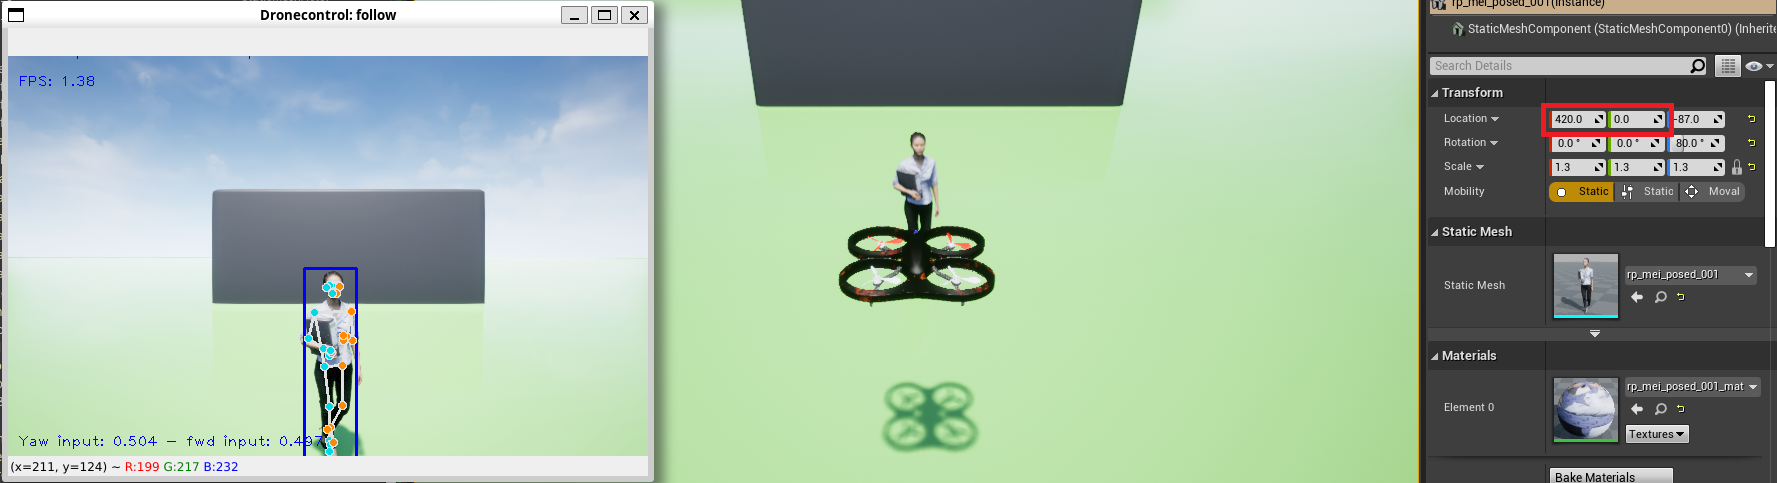
\includegraphics[width=\textwidth, keepaspectratio]{img/pid-3/tune-ref-pos.png}
  \caption{Reference position for the yaw and forward PID controllers. From left to right, the panels show the DroneVisionControl application window, the AirSim simulator world view and the world location of the human model in the simulator. The distance between the vehicle and the person is \unit[420]{cm} in the x direction and 0 in the y direction.}
  \label{fig:tune-start-pos}
\end{figure}


\subsection{Yaw controller}

The initial focus of the tuning process is on the yaw controller. As mentioned earlier, the first step entails determining the sign of the process gain. In this case, the process variable, or input to the controller, corresponds to the normalized position of the detected person in the horizontal axis of the camera's field of view. Here, a value of 0 denotes the person's location at the left edge of the field of view, while a value of 1 signifies their position at the right edge. When the controller generates a positive output, it results in a positive yaw velocity, causing the vehicle to rotate in a rightward direction. In response, the person within the camera's field of view shifts to the left, reducing the input to the controller. Given that positive outputs should lead to increasing inputs, the sign of the output velocity needs to be inverted to prevent undesired exponential growth.

A starting position must be established following the sign's determination and preceding any parameter testing. This starting position introduces an offset for the target person model relative to the reference position illustrated in Figure \ref{fig:tune-start-pos}, provoking a step response within the controller. This offset will be \unit[100]{cm} along the y-axis for the yaw controller. Given that the vehicle is positioned at the origin in the simulation environment, the person model should be situated at coordinates $x=420, y=100$ before starting the tuning process, as shown in the rightmost side of Figure \ref{fig:tune-ref-pos-yaw}. In the leftmost panel of Figure \ref{fig:tune-ref-pos-yaw}, the DroneVisionControl application displays an input of 0.64 for the yaw controller at this position. The controller will, therefore, calculate an error of e(t) = 0.5 − 0.62 (setpoint minus
input) at the start of the test.

\begin{figure}[H]
  \centering
  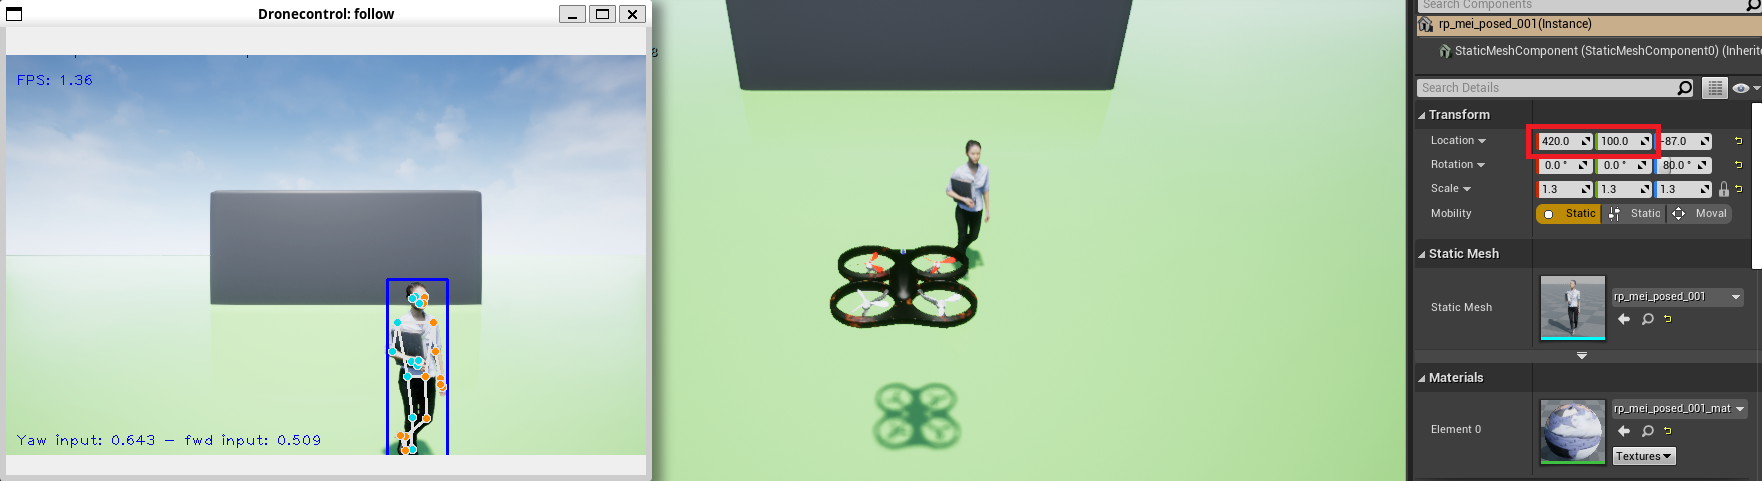
\includegraphics[width=\textwidth, keepaspectratio]{img/pid-3/tune-ref-pos-yaw.png}
  \caption{Starting position of the simulator for tuning the yaw controller. The human model is situated \unit[420]{cm} forward and \unit[100]{cm} to the right of the vehicle model.}
  \label{fig:tune-ref-pos-yaw}
\end{figure}

\subsubsection{Proportional component}

The proportional gain is the first parameter that needs to be tuned. The values chosen to test for $K_P$ range from 25 to 150 in steps of 25. To have a P-only controller during the test, the $K_I$ and $K_D$ components are set to 0. The results of the test are shown in Figures \ref{fig:tune-yaw-prop-io} and \ref{fig:tune-yaw-prop-measures}. The yaw controller's input and output are plotted over time in the first figure (\ref{fig:tune-yaw-prop-io}). On the left side, the input is represented by the calculated error (setpoint minus input position), and on the right side, the output is the velocity sent to the flight controller in degrees per second. The second figure (\ref{fig:tune-yaw-prop-measures}) depicts the corresponding telemetry measurements during the test, with the left graph showing the heading in degrees retrieved from the flight controller and the right graph showing the yaw velocity in degrees per second. The effects of the internal PX4 control mechanisms can be appreciated when comparing these two figures. Thanks to them, the noise introduced by the image detection features is not transmitted to the vehicle's trajectory but smoothed out.

Following the tuning process, the value selected should present a small overshoot initially and then smooth out without undue oscillation. In Figure \ref{fig:tune-yaw-prop-measures}a, the values between 75 and 125 present the initial overshoot, and from $K_P=125$ the oscillations start to be more noticeable. Therefore, the value selected for the proportional gain will be $K_P=100$. 


\begin{figure}[H]
    \begin{minipage}[t]{0.5\linewidth}
        \centering
        \scalebox{0.55}{%% Creator: Matplotlib, PGF backend
%%
%% To include the figure in your LaTeX document, write
%%   \input{<filename>.pgf}
%%
%% Make sure the required packages are loaded in your preamble
%%   \usepackage{pgf}
%%
%% Also ensure that all the required font packages are loaded; for instance,
%% the lmodern package is sometimes necessary when using math font.
%%   \usepackage{lmodern}
%%
%% Figures using additional raster images can only be included by \input if
%% they are in the same directory as the main LaTeX file. For loading figures
%% from other directories you can use the `import` package
%%   \usepackage{import}
%%
%% and then include the figures with
%%   \import{<path to file>}{<filename>.pgf}
%%
%% Matplotlib used the following preamble
%%   \usepackage{fontspec}
%%   \setmainfont{DejaVuSerif.ttf}[Path=\detokenize{/home/lgonz/tfg-aero/tfg-giaa-dronecontrol/venv/lib/python3.8/site-packages/matplotlib/mpl-data/fonts/ttf/}]
%%   \setsansfont{DejaVuSans.ttf}[Path=\detokenize{/home/lgonz/tfg-aero/tfg-giaa-dronecontrol/venv/lib/python3.8/site-packages/matplotlib/mpl-data/fonts/ttf/}]
%%   \setmonofont{DejaVuSansMono.ttf}[Path=\detokenize{/home/lgonz/tfg-aero/tfg-giaa-dronecontrol/venv/lib/python3.8/site-packages/matplotlib/mpl-data/fonts/ttf/}]
%%
\begingroup%
\makeatletter%
\begin{pgfpicture}%
\pgfpathrectangle{\pgfpointorigin}{\pgfqpoint{6.400000in}{4.800000in}}%
\pgfusepath{use as bounding box, clip}%
\begin{pgfscope}%
\pgfsetbuttcap%
\pgfsetmiterjoin%
\definecolor{currentfill}{rgb}{1.000000,1.000000,1.000000}%
\pgfsetfillcolor{currentfill}%
\pgfsetlinewidth{0.000000pt}%
\definecolor{currentstroke}{rgb}{1.000000,1.000000,1.000000}%
\pgfsetstrokecolor{currentstroke}%
\pgfsetdash{}{0pt}%
\pgfpathmoveto{\pgfqpoint{0.000000in}{0.000000in}}%
\pgfpathlineto{\pgfqpoint{6.400000in}{0.000000in}}%
\pgfpathlineto{\pgfqpoint{6.400000in}{4.800000in}}%
\pgfpathlineto{\pgfqpoint{0.000000in}{4.800000in}}%
\pgfpathlineto{\pgfqpoint{0.000000in}{0.000000in}}%
\pgfpathclose%
\pgfusepath{fill}%
\end{pgfscope}%
\begin{pgfscope}%
\pgfsetbuttcap%
\pgfsetmiterjoin%
\definecolor{currentfill}{rgb}{1.000000,1.000000,1.000000}%
\pgfsetfillcolor{currentfill}%
\pgfsetlinewidth{0.000000pt}%
\definecolor{currentstroke}{rgb}{0.000000,0.000000,0.000000}%
\pgfsetstrokecolor{currentstroke}%
\pgfsetstrokeopacity{0.000000}%
\pgfsetdash{}{0pt}%
\pgfpathmoveto{\pgfqpoint{0.800000in}{0.528000in}}%
\pgfpathlineto{\pgfqpoint{5.760000in}{0.528000in}}%
\pgfpathlineto{\pgfqpoint{5.760000in}{4.224000in}}%
\pgfpathlineto{\pgfqpoint{0.800000in}{4.224000in}}%
\pgfpathlineto{\pgfqpoint{0.800000in}{0.528000in}}%
\pgfpathclose%
\pgfusepath{fill}%
\end{pgfscope}%
\begin{pgfscope}%
\pgfpathrectangle{\pgfqpoint{0.800000in}{0.528000in}}{\pgfqpoint{4.960000in}{3.696000in}}%
\pgfusepath{clip}%
\pgfsetrectcap%
\pgfsetroundjoin%
\pgfsetlinewidth{0.803000pt}%
\definecolor{currentstroke}{rgb}{0.690196,0.690196,0.690196}%
\pgfsetstrokecolor{currentstroke}%
\pgfsetdash{}{0pt}%
\pgfpathmoveto{\pgfqpoint{1.025455in}{0.528000in}}%
\pgfpathlineto{\pgfqpoint{1.025455in}{4.224000in}}%
\pgfusepath{stroke}%
\end{pgfscope}%
\begin{pgfscope}%
\pgfsetbuttcap%
\pgfsetroundjoin%
\definecolor{currentfill}{rgb}{0.000000,0.000000,0.000000}%
\pgfsetfillcolor{currentfill}%
\pgfsetlinewidth{0.803000pt}%
\definecolor{currentstroke}{rgb}{0.000000,0.000000,0.000000}%
\pgfsetstrokecolor{currentstroke}%
\pgfsetdash{}{0pt}%
\pgfsys@defobject{currentmarker}{\pgfqpoint{0.000000in}{-0.048611in}}{\pgfqpoint{0.000000in}{0.000000in}}{%
\pgfpathmoveto{\pgfqpoint{0.000000in}{0.000000in}}%
\pgfpathlineto{\pgfqpoint{0.000000in}{-0.048611in}}%
\pgfusepath{stroke,fill}%
}%
\begin{pgfscope}%
\pgfsys@transformshift{1.025455in}{0.528000in}%
\pgfsys@useobject{currentmarker}{}%
\end{pgfscope}%
\end{pgfscope}%
\begin{pgfscope}%
\definecolor{textcolor}{rgb}{0.000000,0.000000,0.000000}%
\pgfsetstrokecolor{textcolor}%
\pgfsetfillcolor{textcolor}%
\pgftext[x=1.025455in,y=0.430778in,,top]{\color{textcolor}\sffamily\fontsize{10.000000}{12.000000}\selectfont 0}%
\end{pgfscope}%
\begin{pgfscope}%
\pgfpathrectangle{\pgfqpoint{0.800000in}{0.528000in}}{\pgfqpoint{4.960000in}{3.696000in}}%
\pgfusepath{clip}%
\pgfsetrectcap%
\pgfsetroundjoin%
\pgfsetlinewidth{0.803000pt}%
\definecolor{currentstroke}{rgb}{0.690196,0.690196,0.690196}%
\pgfsetstrokecolor{currentstroke}%
\pgfsetdash{}{0pt}%
\pgfpathmoveto{\pgfqpoint{1.776110in}{0.528000in}}%
\pgfpathlineto{\pgfqpoint{1.776110in}{4.224000in}}%
\pgfusepath{stroke}%
\end{pgfscope}%
\begin{pgfscope}%
\pgfsetbuttcap%
\pgfsetroundjoin%
\definecolor{currentfill}{rgb}{0.000000,0.000000,0.000000}%
\pgfsetfillcolor{currentfill}%
\pgfsetlinewidth{0.803000pt}%
\definecolor{currentstroke}{rgb}{0.000000,0.000000,0.000000}%
\pgfsetstrokecolor{currentstroke}%
\pgfsetdash{}{0pt}%
\pgfsys@defobject{currentmarker}{\pgfqpoint{0.000000in}{-0.048611in}}{\pgfqpoint{0.000000in}{0.000000in}}{%
\pgfpathmoveto{\pgfqpoint{0.000000in}{0.000000in}}%
\pgfpathlineto{\pgfqpoint{0.000000in}{-0.048611in}}%
\pgfusepath{stroke,fill}%
}%
\begin{pgfscope}%
\pgfsys@transformshift{1.776110in}{0.528000in}%
\pgfsys@useobject{currentmarker}{}%
\end{pgfscope}%
\end{pgfscope}%
\begin{pgfscope}%
\definecolor{textcolor}{rgb}{0.000000,0.000000,0.000000}%
\pgfsetstrokecolor{textcolor}%
\pgfsetfillcolor{textcolor}%
\pgftext[x=1.776110in,y=0.430778in,,top]{\color{textcolor}\sffamily\fontsize{10.000000}{12.000000}\selectfont 5}%
\end{pgfscope}%
\begin{pgfscope}%
\pgfpathrectangle{\pgfqpoint{0.800000in}{0.528000in}}{\pgfqpoint{4.960000in}{3.696000in}}%
\pgfusepath{clip}%
\pgfsetrectcap%
\pgfsetroundjoin%
\pgfsetlinewidth{0.803000pt}%
\definecolor{currentstroke}{rgb}{0.690196,0.690196,0.690196}%
\pgfsetstrokecolor{currentstroke}%
\pgfsetdash{}{0pt}%
\pgfpathmoveto{\pgfqpoint{2.526765in}{0.528000in}}%
\pgfpathlineto{\pgfqpoint{2.526765in}{4.224000in}}%
\pgfusepath{stroke}%
\end{pgfscope}%
\begin{pgfscope}%
\pgfsetbuttcap%
\pgfsetroundjoin%
\definecolor{currentfill}{rgb}{0.000000,0.000000,0.000000}%
\pgfsetfillcolor{currentfill}%
\pgfsetlinewidth{0.803000pt}%
\definecolor{currentstroke}{rgb}{0.000000,0.000000,0.000000}%
\pgfsetstrokecolor{currentstroke}%
\pgfsetdash{}{0pt}%
\pgfsys@defobject{currentmarker}{\pgfqpoint{0.000000in}{-0.048611in}}{\pgfqpoint{0.000000in}{0.000000in}}{%
\pgfpathmoveto{\pgfqpoint{0.000000in}{0.000000in}}%
\pgfpathlineto{\pgfqpoint{0.000000in}{-0.048611in}}%
\pgfusepath{stroke,fill}%
}%
\begin{pgfscope}%
\pgfsys@transformshift{2.526765in}{0.528000in}%
\pgfsys@useobject{currentmarker}{}%
\end{pgfscope}%
\end{pgfscope}%
\begin{pgfscope}%
\definecolor{textcolor}{rgb}{0.000000,0.000000,0.000000}%
\pgfsetstrokecolor{textcolor}%
\pgfsetfillcolor{textcolor}%
\pgftext[x=2.526765in,y=0.430778in,,top]{\color{textcolor}\sffamily\fontsize{10.000000}{12.000000}\selectfont 10}%
\end{pgfscope}%
\begin{pgfscope}%
\pgfpathrectangle{\pgfqpoint{0.800000in}{0.528000in}}{\pgfqpoint{4.960000in}{3.696000in}}%
\pgfusepath{clip}%
\pgfsetrectcap%
\pgfsetroundjoin%
\pgfsetlinewidth{0.803000pt}%
\definecolor{currentstroke}{rgb}{0.690196,0.690196,0.690196}%
\pgfsetstrokecolor{currentstroke}%
\pgfsetdash{}{0pt}%
\pgfpathmoveto{\pgfqpoint{3.277420in}{0.528000in}}%
\pgfpathlineto{\pgfqpoint{3.277420in}{4.224000in}}%
\pgfusepath{stroke}%
\end{pgfscope}%
\begin{pgfscope}%
\pgfsetbuttcap%
\pgfsetroundjoin%
\definecolor{currentfill}{rgb}{0.000000,0.000000,0.000000}%
\pgfsetfillcolor{currentfill}%
\pgfsetlinewidth{0.803000pt}%
\definecolor{currentstroke}{rgb}{0.000000,0.000000,0.000000}%
\pgfsetstrokecolor{currentstroke}%
\pgfsetdash{}{0pt}%
\pgfsys@defobject{currentmarker}{\pgfqpoint{0.000000in}{-0.048611in}}{\pgfqpoint{0.000000in}{0.000000in}}{%
\pgfpathmoveto{\pgfqpoint{0.000000in}{0.000000in}}%
\pgfpathlineto{\pgfqpoint{0.000000in}{-0.048611in}}%
\pgfusepath{stroke,fill}%
}%
\begin{pgfscope}%
\pgfsys@transformshift{3.277420in}{0.528000in}%
\pgfsys@useobject{currentmarker}{}%
\end{pgfscope}%
\end{pgfscope}%
\begin{pgfscope}%
\definecolor{textcolor}{rgb}{0.000000,0.000000,0.000000}%
\pgfsetstrokecolor{textcolor}%
\pgfsetfillcolor{textcolor}%
\pgftext[x=3.277420in,y=0.430778in,,top]{\color{textcolor}\sffamily\fontsize{10.000000}{12.000000}\selectfont 15}%
\end{pgfscope}%
\begin{pgfscope}%
\pgfpathrectangle{\pgfqpoint{0.800000in}{0.528000in}}{\pgfqpoint{4.960000in}{3.696000in}}%
\pgfusepath{clip}%
\pgfsetrectcap%
\pgfsetroundjoin%
\pgfsetlinewidth{0.803000pt}%
\definecolor{currentstroke}{rgb}{0.690196,0.690196,0.690196}%
\pgfsetstrokecolor{currentstroke}%
\pgfsetdash{}{0pt}%
\pgfpathmoveto{\pgfqpoint{4.028075in}{0.528000in}}%
\pgfpathlineto{\pgfqpoint{4.028075in}{4.224000in}}%
\pgfusepath{stroke}%
\end{pgfscope}%
\begin{pgfscope}%
\pgfsetbuttcap%
\pgfsetroundjoin%
\definecolor{currentfill}{rgb}{0.000000,0.000000,0.000000}%
\pgfsetfillcolor{currentfill}%
\pgfsetlinewidth{0.803000pt}%
\definecolor{currentstroke}{rgb}{0.000000,0.000000,0.000000}%
\pgfsetstrokecolor{currentstroke}%
\pgfsetdash{}{0pt}%
\pgfsys@defobject{currentmarker}{\pgfqpoint{0.000000in}{-0.048611in}}{\pgfqpoint{0.000000in}{0.000000in}}{%
\pgfpathmoveto{\pgfqpoint{0.000000in}{0.000000in}}%
\pgfpathlineto{\pgfqpoint{0.000000in}{-0.048611in}}%
\pgfusepath{stroke,fill}%
}%
\begin{pgfscope}%
\pgfsys@transformshift{4.028075in}{0.528000in}%
\pgfsys@useobject{currentmarker}{}%
\end{pgfscope}%
\end{pgfscope}%
\begin{pgfscope}%
\definecolor{textcolor}{rgb}{0.000000,0.000000,0.000000}%
\pgfsetstrokecolor{textcolor}%
\pgfsetfillcolor{textcolor}%
\pgftext[x=4.028075in,y=0.430778in,,top]{\color{textcolor}\sffamily\fontsize{10.000000}{12.000000}\selectfont 20}%
\end{pgfscope}%
\begin{pgfscope}%
\pgfpathrectangle{\pgfqpoint{0.800000in}{0.528000in}}{\pgfqpoint{4.960000in}{3.696000in}}%
\pgfusepath{clip}%
\pgfsetrectcap%
\pgfsetroundjoin%
\pgfsetlinewidth{0.803000pt}%
\definecolor{currentstroke}{rgb}{0.690196,0.690196,0.690196}%
\pgfsetstrokecolor{currentstroke}%
\pgfsetdash{}{0pt}%
\pgfpathmoveto{\pgfqpoint{4.778730in}{0.528000in}}%
\pgfpathlineto{\pgfqpoint{4.778730in}{4.224000in}}%
\pgfusepath{stroke}%
\end{pgfscope}%
\begin{pgfscope}%
\pgfsetbuttcap%
\pgfsetroundjoin%
\definecolor{currentfill}{rgb}{0.000000,0.000000,0.000000}%
\pgfsetfillcolor{currentfill}%
\pgfsetlinewidth{0.803000pt}%
\definecolor{currentstroke}{rgb}{0.000000,0.000000,0.000000}%
\pgfsetstrokecolor{currentstroke}%
\pgfsetdash{}{0pt}%
\pgfsys@defobject{currentmarker}{\pgfqpoint{0.000000in}{-0.048611in}}{\pgfqpoint{0.000000in}{0.000000in}}{%
\pgfpathmoveto{\pgfqpoint{0.000000in}{0.000000in}}%
\pgfpathlineto{\pgfqpoint{0.000000in}{-0.048611in}}%
\pgfusepath{stroke,fill}%
}%
\begin{pgfscope}%
\pgfsys@transformshift{4.778730in}{0.528000in}%
\pgfsys@useobject{currentmarker}{}%
\end{pgfscope}%
\end{pgfscope}%
\begin{pgfscope}%
\definecolor{textcolor}{rgb}{0.000000,0.000000,0.000000}%
\pgfsetstrokecolor{textcolor}%
\pgfsetfillcolor{textcolor}%
\pgftext[x=4.778730in,y=0.430778in,,top]{\color{textcolor}\sffamily\fontsize{10.000000}{12.000000}\selectfont 25}%
\end{pgfscope}%
\begin{pgfscope}%
\pgfpathrectangle{\pgfqpoint{0.800000in}{0.528000in}}{\pgfqpoint{4.960000in}{3.696000in}}%
\pgfusepath{clip}%
\pgfsetrectcap%
\pgfsetroundjoin%
\pgfsetlinewidth{0.803000pt}%
\definecolor{currentstroke}{rgb}{0.690196,0.690196,0.690196}%
\pgfsetstrokecolor{currentstroke}%
\pgfsetdash{}{0pt}%
\pgfpathmoveto{\pgfqpoint{5.529385in}{0.528000in}}%
\pgfpathlineto{\pgfqpoint{5.529385in}{4.224000in}}%
\pgfusepath{stroke}%
\end{pgfscope}%
\begin{pgfscope}%
\pgfsetbuttcap%
\pgfsetroundjoin%
\definecolor{currentfill}{rgb}{0.000000,0.000000,0.000000}%
\pgfsetfillcolor{currentfill}%
\pgfsetlinewidth{0.803000pt}%
\definecolor{currentstroke}{rgb}{0.000000,0.000000,0.000000}%
\pgfsetstrokecolor{currentstroke}%
\pgfsetdash{}{0pt}%
\pgfsys@defobject{currentmarker}{\pgfqpoint{0.000000in}{-0.048611in}}{\pgfqpoint{0.000000in}{0.000000in}}{%
\pgfpathmoveto{\pgfqpoint{0.000000in}{0.000000in}}%
\pgfpathlineto{\pgfqpoint{0.000000in}{-0.048611in}}%
\pgfusepath{stroke,fill}%
}%
\begin{pgfscope}%
\pgfsys@transformshift{5.529385in}{0.528000in}%
\pgfsys@useobject{currentmarker}{}%
\end{pgfscope}%
\end{pgfscope}%
\begin{pgfscope}%
\definecolor{textcolor}{rgb}{0.000000,0.000000,0.000000}%
\pgfsetstrokecolor{textcolor}%
\pgfsetfillcolor{textcolor}%
\pgftext[x=5.529385in,y=0.430778in,,top]{\color{textcolor}\sffamily\fontsize{10.000000}{12.000000}\selectfont 30}%
\end{pgfscope}%
\begin{pgfscope}%
\definecolor{textcolor}{rgb}{0.000000,0.000000,0.000000}%
\pgfsetstrokecolor{textcolor}%
\pgfsetfillcolor{textcolor}%
\pgftext[x=3.280000in,y=0.240809in,,top]{\color{textcolor}\sffamily\fontsize{10.000000}{12.000000}\selectfont time [s]}%
\end{pgfscope}%
\begin{pgfscope}%
\pgfpathrectangle{\pgfqpoint{0.800000in}{0.528000in}}{\pgfqpoint{4.960000in}{3.696000in}}%
\pgfusepath{clip}%
\pgfsetrectcap%
\pgfsetroundjoin%
\pgfsetlinewidth{0.803000pt}%
\definecolor{currentstroke}{rgb}{0.690196,0.690196,0.690196}%
\pgfsetstrokecolor{currentstroke}%
\pgfsetdash{}{0pt}%
\pgfpathmoveto{\pgfqpoint{0.800000in}{0.784351in}}%
\pgfpathlineto{\pgfqpoint{5.760000in}{0.784351in}}%
\pgfusepath{stroke}%
\end{pgfscope}%
\begin{pgfscope}%
\pgfsetbuttcap%
\pgfsetroundjoin%
\definecolor{currentfill}{rgb}{0.000000,0.000000,0.000000}%
\pgfsetfillcolor{currentfill}%
\pgfsetlinewidth{0.803000pt}%
\definecolor{currentstroke}{rgb}{0.000000,0.000000,0.000000}%
\pgfsetstrokecolor{currentstroke}%
\pgfsetdash{}{0pt}%
\pgfsys@defobject{currentmarker}{\pgfqpoint{-0.048611in}{0.000000in}}{\pgfqpoint{-0.000000in}{0.000000in}}{%
\pgfpathmoveto{\pgfqpoint{-0.000000in}{0.000000in}}%
\pgfpathlineto{\pgfqpoint{-0.048611in}{0.000000in}}%
\pgfusepath{stroke,fill}%
}%
\begin{pgfscope}%
\pgfsys@transformshift{0.800000in}{0.784351in}%
\pgfsys@useobject{currentmarker}{}%
\end{pgfscope}%
\end{pgfscope}%
\begin{pgfscope}%
\definecolor{textcolor}{rgb}{0.000000,0.000000,0.000000}%
\pgfsetstrokecolor{textcolor}%
\pgfsetfillcolor{textcolor}%
\pgftext[x=0.197143in, y=0.731590in, left, base]{\color{textcolor}\sffamily\fontsize{10.000000}{12.000000}\selectfont \ensuremath{-}0.150}%
\end{pgfscope}%
\begin{pgfscope}%
\pgfpathrectangle{\pgfqpoint{0.800000in}{0.528000in}}{\pgfqpoint{4.960000in}{3.696000in}}%
\pgfusepath{clip}%
\pgfsetrectcap%
\pgfsetroundjoin%
\pgfsetlinewidth{0.803000pt}%
\definecolor{currentstroke}{rgb}{0.690196,0.690196,0.690196}%
\pgfsetstrokecolor{currentstroke}%
\pgfsetdash{}{0pt}%
\pgfpathmoveto{\pgfqpoint{0.800000in}{1.285329in}}%
\pgfpathlineto{\pgfqpoint{5.760000in}{1.285329in}}%
\pgfusepath{stroke}%
\end{pgfscope}%
\begin{pgfscope}%
\pgfsetbuttcap%
\pgfsetroundjoin%
\definecolor{currentfill}{rgb}{0.000000,0.000000,0.000000}%
\pgfsetfillcolor{currentfill}%
\pgfsetlinewidth{0.803000pt}%
\definecolor{currentstroke}{rgb}{0.000000,0.000000,0.000000}%
\pgfsetstrokecolor{currentstroke}%
\pgfsetdash{}{0pt}%
\pgfsys@defobject{currentmarker}{\pgfqpoint{-0.048611in}{0.000000in}}{\pgfqpoint{-0.000000in}{0.000000in}}{%
\pgfpathmoveto{\pgfqpoint{-0.000000in}{0.000000in}}%
\pgfpathlineto{\pgfqpoint{-0.048611in}{0.000000in}}%
\pgfusepath{stroke,fill}%
}%
\begin{pgfscope}%
\pgfsys@transformshift{0.800000in}{1.285329in}%
\pgfsys@useobject{currentmarker}{}%
\end{pgfscope}%
\end{pgfscope}%
\begin{pgfscope}%
\definecolor{textcolor}{rgb}{0.000000,0.000000,0.000000}%
\pgfsetstrokecolor{textcolor}%
\pgfsetfillcolor{textcolor}%
\pgftext[x=0.197143in, y=1.232568in, left, base]{\color{textcolor}\sffamily\fontsize{10.000000}{12.000000}\selectfont \ensuremath{-}0.125}%
\end{pgfscope}%
\begin{pgfscope}%
\pgfpathrectangle{\pgfqpoint{0.800000in}{0.528000in}}{\pgfqpoint{4.960000in}{3.696000in}}%
\pgfusepath{clip}%
\pgfsetrectcap%
\pgfsetroundjoin%
\pgfsetlinewidth{0.803000pt}%
\definecolor{currentstroke}{rgb}{0.690196,0.690196,0.690196}%
\pgfsetstrokecolor{currentstroke}%
\pgfsetdash{}{0pt}%
\pgfpathmoveto{\pgfqpoint{0.800000in}{1.786308in}}%
\pgfpathlineto{\pgfqpoint{5.760000in}{1.786308in}}%
\pgfusepath{stroke}%
\end{pgfscope}%
\begin{pgfscope}%
\pgfsetbuttcap%
\pgfsetroundjoin%
\definecolor{currentfill}{rgb}{0.000000,0.000000,0.000000}%
\pgfsetfillcolor{currentfill}%
\pgfsetlinewidth{0.803000pt}%
\definecolor{currentstroke}{rgb}{0.000000,0.000000,0.000000}%
\pgfsetstrokecolor{currentstroke}%
\pgfsetdash{}{0pt}%
\pgfsys@defobject{currentmarker}{\pgfqpoint{-0.048611in}{0.000000in}}{\pgfqpoint{-0.000000in}{0.000000in}}{%
\pgfpathmoveto{\pgfqpoint{-0.000000in}{0.000000in}}%
\pgfpathlineto{\pgfqpoint{-0.048611in}{0.000000in}}%
\pgfusepath{stroke,fill}%
}%
\begin{pgfscope}%
\pgfsys@transformshift{0.800000in}{1.786308in}%
\pgfsys@useobject{currentmarker}{}%
\end{pgfscope}%
\end{pgfscope}%
\begin{pgfscope}%
\definecolor{textcolor}{rgb}{0.000000,0.000000,0.000000}%
\pgfsetstrokecolor{textcolor}%
\pgfsetfillcolor{textcolor}%
\pgftext[x=0.197143in, y=1.733546in, left, base]{\color{textcolor}\sffamily\fontsize{10.000000}{12.000000}\selectfont \ensuremath{-}0.100}%
\end{pgfscope}%
\begin{pgfscope}%
\pgfpathrectangle{\pgfqpoint{0.800000in}{0.528000in}}{\pgfqpoint{4.960000in}{3.696000in}}%
\pgfusepath{clip}%
\pgfsetrectcap%
\pgfsetroundjoin%
\pgfsetlinewidth{0.803000pt}%
\definecolor{currentstroke}{rgb}{0.690196,0.690196,0.690196}%
\pgfsetstrokecolor{currentstroke}%
\pgfsetdash{}{0pt}%
\pgfpathmoveto{\pgfqpoint{0.800000in}{2.287286in}}%
\pgfpathlineto{\pgfqpoint{5.760000in}{2.287286in}}%
\pgfusepath{stroke}%
\end{pgfscope}%
\begin{pgfscope}%
\pgfsetbuttcap%
\pgfsetroundjoin%
\definecolor{currentfill}{rgb}{0.000000,0.000000,0.000000}%
\pgfsetfillcolor{currentfill}%
\pgfsetlinewidth{0.803000pt}%
\definecolor{currentstroke}{rgb}{0.000000,0.000000,0.000000}%
\pgfsetstrokecolor{currentstroke}%
\pgfsetdash{}{0pt}%
\pgfsys@defobject{currentmarker}{\pgfqpoint{-0.048611in}{0.000000in}}{\pgfqpoint{-0.000000in}{0.000000in}}{%
\pgfpathmoveto{\pgfqpoint{-0.000000in}{0.000000in}}%
\pgfpathlineto{\pgfqpoint{-0.048611in}{0.000000in}}%
\pgfusepath{stroke,fill}%
}%
\begin{pgfscope}%
\pgfsys@transformshift{0.800000in}{2.287286in}%
\pgfsys@useobject{currentmarker}{}%
\end{pgfscope}%
\end{pgfscope}%
\begin{pgfscope}%
\definecolor{textcolor}{rgb}{0.000000,0.000000,0.000000}%
\pgfsetstrokecolor{textcolor}%
\pgfsetfillcolor{textcolor}%
\pgftext[x=0.197143in, y=2.234524in, left, base]{\color{textcolor}\sffamily\fontsize{10.000000}{12.000000}\selectfont \ensuremath{-}0.075}%
\end{pgfscope}%
\begin{pgfscope}%
\pgfpathrectangle{\pgfqpoint{0.800000in}{0.528000in}}{\pgfqpoint{4.960000in}{3.696000in}}%
\pgfusepath{clip}%
\pgfsetrectcap%
\pgfsetroundjoin%
\pgfsetlinewidth{0.803000pt}%
\definecolor{currentstroke}{rgb}{0.690196,0.690196,0.690196}%
\pgfsetstrokecolor{currentstroke}%
\pgfsetdash{}{0pt}%
\pgfpathmoveto{\pgfqpoint{0.800000in}{2.788264in}}%
\pgfpathlineto{\pgfqpoint{5.760000in}{2.788264in}}%
\pgfusepath{stroke}%
\end{pgfscope}%
\begin{pgfscope}%
\pgfsetbuttcap%
\pgfsetroundjoin%
\definecolor{currentfill}{rgb}{0.000000,0.000000,0.000000}%
\pgfsetfillcolor{currentfill}%
\pgfsetlinewidth{0.803000pt}%
\definecolor{currentstroke}{rgb}{0.000000,0.000000,0.000000}%
\pgfsetstrokecolor{currentstroke}%
\pgfsetdash{}{0pt}%
\pgfsys@defobject{currentmarker}{\pgfqpoint{-0.048611in}{0.000000in}}{\pgfqpoint{-0.000000in}{0.000000in}}{%
\pgfpathmoveto{\pgfqpoint{-0.000000in}{0.000000in}}%
\pgfpathlineto{\pgfqpoint{-0.048611in}{0.000000in}}%
\pgfusepath{stroke,fill}%
}%
\begin{pgfscope}%
\pgfsys@transformshift{0.800000in}{2.788264in}%
\pgfsys@useobject{currentmarker}{}%
\end{pgfscope}%
\end{pgfscope}%
\begin{pgfscope}%
\definecolor{textcolor}{rgb}{0.000000,0.000000,0.000000}%
\pgfsetstrokecolor{textcolor}%
\pgfsetfillcolor{textcolor}%
\pgftext[x=0.197143in, y=2.735503in, left, base]{\color{textcolor}\sffamily\fontsize{10.000000}{12.000000}\selectfont \ensuremath{-}0.050}%
\end{pgfscope}%
\begin{pgfscope}%
\pgfpathrectangle{\pgfqpoint{0.800000in}{0.528000in}}{\pgfqpoint{4.960000in}{3.696000in}}%
\pgfusepath{clip}%
\pgfsetrectcap%
\pgfsetroundjoin%
\pgfsetlinewidth{0.803000pt}%
\definecolor{currentstroke}{rgb}{0.690196,0.690196,0.690196}%
\pgfsetstrokecolor{currentstroke}%
\pgfsetdash{}{0pt}%
\pgfpathmoveto{\pgfqpoint{0.800000in}{3.289242in}}%
\pgfpathlineto{\pgfqpoint{5.760000in}{3.289242in}}%
\pgfusepath{stroke}%
\end{pgfscope}%
\begin{pgfscope}%
\pgfsetbuttcap%
\pgfsetroundjoin%
\definecolor{currentfill}{rgb}{0.000000,0.000000,0.000000}%
\pgfsetfillcolor{currentfill}%
\pgfsetlinewidth{0.803000pt}%
\definecolor{currentstroke}{rgb}{0.000000,0.000000,0.000000}%
\pgfsetstrokecolor{currentstroke}%
\pgfsetdash{}{0pt}%
\pgfsys@defobject{currentmarker}{\pgfqpoint{-0.048611in}{0.000000in}}{\pgfqpoint{-0.000000in}{0.000000in}}{%
\pgfpathmoveto{\pgfqpoint{-0.000000in}{0.000000in}}%
\pgfpathlineto{\pgfqpoint{-0.048611in}{0.000000in}}%
\pgfusepath{stroke,fill}%
}%
\begin{pgfscope}%
\pgfsys@transformshift{0.800000in}{3.289242in}%
\pgfsys@useobject{currentmarker}{}%
\end{pgfscope}%
\end{pgfscope}%
\begin{pgfscope}%
\definecolor{textcolor}{rgb}{0.000000,0.000000,0.000000}%
\pgfsetstrokecolor{textcolor}%
\pgfsetfillcolor{textcolor}%
\pgftext[x=0.197143in, y=3.236481in, left, base]{\color{textcolor}\sffamily\fontsize{10.000000}{12.000000}\selectfont \ensuremath{-}0.025}%
\end{pgfscope}%
\begin{pgfscope}%
\pgfpathrectangle{\pgfqpoint{0.800000in}{0.528000in}}{\pgfqpoint{4.960000in}{3.696000in}}%
\pgfusepath{clip}%
\pgfsetrectcap%
\pgfsetroundjoin%
\pgfsetlinewidth{0.803000pt}%
\definecolor{currentstroke}{rgb}{0.690196,0.690196,0.690196}%
\pgfsetstrokecolor{currentstroke}%
\pgfsetdash{}{0pt}%
\pgfpathmoveto{\pgfqpoint{0.800000in}{3.790221in}}%
\pgfpathlineto{\pgfqpoint{5.760000in}{3.790221in}}%
\pgfusepath{stroke}%
\end{pgfscope}%
\begin{pgfscope}%
\pgfsetbuttcap%
\pgfsetroundjoin%
\definecolor{currentfill}{rgb}{0.000000,0.000000,0.000000}%
\pgfsetfillcolor{currentfill}%
\pgfsetlinewidth{0.803000pt}%
\definecolor{currentstroke}{rgb}{0.000000,0.000000,0.000000}%
\pgfsetstrokecolor{currentstroke}%
\pgfsetdash{}{0pt}%
\pgfsys@defobject{currentmarker}{\pgfqpoint{-0.048611in}{0.000000in}}{\pgfqpoint{-0.000000in}{0.000000in}}{%
\pgfpathmoveto{\pgfqpoint{-0.000000in}{0.000000in}}%
\pgfpathlineto{\pgfqpoint{-0.048611in}{0.000000in}}%
\pgfusepath{stroke,fill}%
}%
\begin{pgfscope}%
\pgfsys@transformshift{0.800000in}{3.790221in}%
\pgfsys@useobject{currentmarker}{}%
\end{pgfscope}%
\end{pgfscope}%
\begin{pgfscope}%
\definecolor{textcolor}{rgb}{0.000000,0.000000,0.000000}%
\pgfsetstrokecolor{textcolor}%
\pgfsetfillcolor{textcolor}%
\pgftext[x=0.305168in, y=3.737459in, left, base]{\color{textcolor}\sffamily\fontsize{10.000000}{12.000000}\selectfont 0.000}%
\end{pgfscope}%
\begin{pgfscope}%
\definecolor{textcolor}{rgb}{0.000000,0.000000,0.000000}%
\pgfsetstrokecolor{textcolor}%
\pgfsetfillcolor{textcolor}%
\pgftext[x=0.141587in,y=2.376000in,,bottom,rotate=90.000000]{\color{textcolor}\sffamily\fontsize{10.000000}{12.000000}\selectfont Computed error [-]}%
\end{pgfscope}%
\begin{pgfscope}%
\pgfpathrectangle{\pgfqpoint{0.800000in}{0.528000in}}{\pgfqpoint{4.960000in}{3.696000in}}%
\pgfusepath{clip}%
\pgfsetrectcap%
\pgfsetroundjoin%
\pgfsetlinewidth{1.505625pt}%
\definecolor{currentstroke}{rgb}{0.121569,0.466667,0.705882}%
\pgfsetstrokecolor{currentstroke}%
\pgfsetdash{}{0pt}%
\pgfpathmoveto{\pgfqpoint{1.025455in}{0.872516in}}%
\pgfpathlineto{\pgfqpoint{1.079516in}{0.883000in}}%
\pgfpathlineto{\pgfqpoint{1.133631in}{1.013667in}}%
\pgfpathlineto{\pgfqpoint{1.188238in}{1.283523in}}%
\pgfpathlineto{\pgfqpoint{1.242140in}{1.523027in}}%
\pgfpathlineto{\pgfqpoint{1.296574in}{1.874420in}}%
\pgfpathlineto{\pgfqpoint{1.350975in}{2.065229in}}%
\pgfpathlineto{\pgfqpoint{1.405198in}{2.242107in}}%
\pgfpathlineto{\pgfqpoint{1.459421in}{2.414761in}}%
\pgfpathlineto{\pgfqpoint{1.515483in}{2.554916in}}%
\pgfpathlineto{\pgfqpoint{1.568808in}{2.714734in}}%
\pgfpathlineto{\pgfqpoint{1.622750in}{2.923740in}}%
\pgfpathlineto{\pgfqpoint{1.676811in}{3.005521in}}%
\pgfpathlineto{\pgfqpoint{1.731075in}{2.993491in}}%
\pgfpathlineto{\pgfqpoint{1.785353in}{3.019440in}}%
\pgfpathlineto{\pgfqpoint{1.839997in}{3.076945in}}%
\pgfpathlineto{\pgfqpoint{1.893926in}{3.094364in}}%
\pgfpathlineto{\pgfqpoint{1.948159in}{3.157087in}}%
\pgfpathlineto{\pgfqpoint{2.002121in}{3.204057in}}%
\pgfpathlineto{\pgfqpoint{2.056390in}{3.230878in}}%
\pgfpathlineto{\pgfqpoint{2.110578in}{3.286701in}}%
\pgfpathlineto{\pgfqpoint{2.166151in}{3.319833in}}%
\pgfpathlineto{\pgfqpoint{2.219555in}{3.366243in}}%
\pgfpathlineto{\pgfqpoint{2.273494in}{3.378412in}}%
\pgfpathlineto{\pgfqpoint{2.327782in}{3.458771in}}%
\pgfpathlineto{\pgfqpoint{2.381966in}{3.425521in}}%
\pgfpathlineto{\pgfqpoint{2.436095in}{3.436238in}}%
\pgfpathlineto{\pgfqpoint{2.491009in}{3.446751in}}%
\pgfpathlineto{\pgfqpoint{2.545051in}{3.508100in}}%
\pgfpathlineto{\pgfqpoint{2.598813in}{3.504367in}}%
\pgfpathlineto{\pgfqpoint{2.653291in}{3.526245in}}%
\pgfpathlineto{\pgfqpoint{2.707761in}{3.544353in}}%
\pgfpathlineto{\pgfqpoint{2.763674in}{3.571050in}}%
\pgfpathlineto{\pgfqpoint{2.817407in}{3.550455in}}%
\pgfpathlineto{\pgfqpoint{2.871159in}{3.680423in}}%
\pgfpathlineto{\pgfqpoint{2.925754in}{3.658072in}}%
\pgfpathlineto{\pgfqpoint{2.979889in}{3.722978in}}%
\pgfpathlineto{\pgfqpoint{3.034129in}{3.700188in}}%
\pgfpathlineto{\pgfqpoint{3.088657in}{3.676009in}}%
\pgfpathlineto{\pgfqpoint{3.143340in}{3.652065in}}%
\pgfpathlineto{\pgfqpoint{3.197433in}{3.654560in}}%
\pgfpathlineto{\pgfqpoint{3.251337in}{3.655636in}}%
\pgfpathlineto{\pgfqpoint{3.305832in}{3.669277in}}%
\pgfpathlineto{\pgfqpoint{3.360094in}{3.680704in}}%
\pgfpathlineto{\pgfqpoint{3.416138in}{3.730385in}}%
\pgfpathlineto{\pgfqpoint{3.469948in}{3.743355in}}%
\pgfpathlineto{\pgfqpoint{3.523506in}{3.729802in}}%
\pgfpathlineto{\pgfqpoint{3.577559in}{3.745602in}}%
\pgfpathlineto{\pgfqpoint{3.631802in}{3.816598in}}%
\pgfpathlineto{\pgfqpoint{3.686217in}{3.822043in}}%
\pgfpathlineto{\pgfqpoint{3.740961in}{3.790693in}}%
\pgfpathlineto{\pgfqpoint{3.795240in}{3.792557in}}%
\pgfpathlineto{\pgfqpoint{3.848840in}{3.754744in}}%
\pgfpathlineto{\pgfqpoint{3.903198in}{3.755899in}}%
\pgfpathlineto{\pgfqpoint{3.957709in}{3.745998in}}%
\pgfpathlineto{\pgfqpoint{4.013191in}{3.843371in}}%
\pgfpathlineto{\pgfqpoint{4.066658in}{3.782304in}}%
\pgfpathlineto{\pgfqpoint{4.120500in}{3.752011in}}%
\pgfpathlineto{\pgfqpoint{4.174705in}{3.750106in}}%
\pgfpathlineto{\pgfqpoint{4.228762in}{3.738224in}}%
\pgfpathlineto{\pgfqpoint{4.283406in}{3.780620in}}%
\pgfpathlineto{\pgfqpoint{4.337890in}{3.760705in}}%
\pgfpathlineto{\pgfqpoint{4.392466in}{3.801957in}}%
\pgfpathlineto{\pgfqpoint{4.446367in}{3.869315in}}%
\pgfpathlineto{\pgfqpoint{4.500751in}{3.878539in}}%
\pgfpathlineto{\pgfqpoint{4.555081in}{3.876890in}}%
\pgfpathlineto{\pgfqpoint{4.609565in}{3.874878in}}%
\pgfpathlineto{\pgfqpoint{4.665173in}{3.819224in}}%
\pgfpathlineto{\pgfqpoint{4.718303in}{3.797076in}}%
\pgfpathlineto{\pgfqpoint{4.773428in}{3.757564in}}%
\pgfpathlineto{\pgfqpoint{4.826762in}{3.743386in}}%
\pgfpathlineto{\pgfqpoint{4.881159in}{3.728224in}}%
\pgfpathlineto{\pgfqpoint{4.935742in}{3.728581in}}%
\pgfpathlineto{\pgfqpoint{4.989944in}{3.807411in}}%
\pgfpathlineto{\pgfqpoint{5.045403in}{3.780004in}}%
\pgfpathlineto{\pgfqpoint{5.099927in}{3.772649in}}%
\pgfpathlineto{\pgfqpoint{5.153386in}{3.761211in}}%
\pgfpathlineto{\pgfqpoint{5.209226in}{3.790922in}}%
\pgfpathlineto{\pgfqpoint{5.262766in}{3.801955in}}%
\pgfpathlineto{\pgfqpoint{5.316868in}{3.802212in}}%
\pgfpathlineto{\pgfqpoint{5.371005in}{3.813901in}}%
\pgfpathlineto{\pgfqpoint{5.425298in}{3.827391in}}%
\pgfpathlineto{\pgfqpoint{5.479539in}{3.834485in}}%
\pgfpathlineto{\pgfqpoint{5.533918in}{3.835498in}}%
\pgfusepath{stroke}%
\end{pgfscope}%
\begin{pgfscope}%
\pgfpathrectangle{\pgfqpoint{0.800000in}{0.528000in}}{\pgfqpoint{4.960000in}{3.696000in}}%
\pgfusepath{clip}%
\pgfsetrectcap%
\pgfsetroundjoin%
\pgfsetlinewidth{1.505625pt}%
\definecolor{currentstroke}{rgb}{1.000000,0.498039,0.054902}%
\pgfsetstrokecolor{currentstroke}%
\pgfsetdash{}{0pt}%
\pgfpathmoveto{\pgfqpoint{1.025455in}{0.707997in}}%
\pgfpathlineto{\pgfqpoint{1.079589in}{0.790628in}}%
\pgfpathlineto{\pgfqpoint{1.133843in}{0.938142in}}%
\pgfpathlineto{\pgfqpoint{1.188291in}{1.274221in}}%
\pgfpathlineto{\pgfqpoint{1.242258in}{1.640947in}}%
\pgfpathlineto{\pgfqpoint{1.298457in}{2.035388in}}%
\pgfpathlineto{\pgfqpoint{1.351410in}{2.399744in}}%
\pgfpathlineto{\pgfqpoint{1.405608in}{2.776450in}}%
\pgfpathlineto{\pgfqpoint{1.459687in}{3.140371in}}%
\pgfpathlineto{\pgfqpoint{1.513824in}{3.302915in}}%
\pgfpathlineto{\pgfqpoint{1.567990in}{3.447819in}}%
\pgfpathlineto{\pgfqpoint{1.622687in}{3.594476in}}%
\pgfpathlineto{\pgfqpoint{1.677986in}{3.628237in}}%
\pgfpathlineto{\pgfqpoint{1.732045in}{3.612730in}}%
\pgfpathlineto{\pgfqpoint{1.786270in}{3.637676in}}%
\pgfpathlineto{\pgfqpoint{1.840483in}{3.651760in}}%
\pgfpathlineto{\pgfqpoint{1.894850in}{3.688699in}}%
\pgfpathlineto{\pgfqpoint{1.951417in}{3.666577in}}%
\pgfpathlineto{\pgfqpoint{2.004788in}{3.655312in}}%
\pgfpathlineto{\pgfqpoint{2.059131in}{3.731578in}}%
\pgfpathlineto{\pgfqpoint{2.113176in}{3.695803in}}%
\pgfpathlineto{\pgfqpoint{2.167381in}{3.690282in}}%
\pgfpathlineto{\pgfqpoint{2.221700in}{3.739925in}}%
\pgfpathlineto{\pgfqpoint{2.275856in}{3.728022in}}%
\pgfpathlineto{\pgfqpoint{2.330368in}{3.714492in}}%
\pgfpathlineto{\pgfqpoint{2.384115in}{3.706126in}}%
\pgfpathlineto{\pgfqpoint{2.438457in}{3.697329in}}%
\pgfpathlineto{\pgfqpoint{2.492833in}{3.690511in}}%
\pgfpathlineto{\pgfqpoint{2.547091in}{3.709567in}}%
\pgfpathlineto{\pgfqpoint{2.602432in}{3.705391in}}%
\pgfpathlineto{\pgfqpoint{2.657086in}{3.732411in}}%
\pgfpathlineto{\pgfqpoint{2.709964in}{3.732646in}}%
\pgfpathlineto{\pgfqpoint{2.764261in}{3.733459in}}%
\pgfpathlineto{\pgfqpoint{2.818808in}{3.779302in}}%
\pgfpathlineto{\pgfqpoint{2.873067in}{3.740390in}}%
\pgfpathlineto{\pgfqpoint{2.927345in}{3.747040in}}%
\pgfpathlineto{\pgfqpoint{2.981611in}{3.755735in}}%
\pgfpathlineto{\pgfqpoint{3.035468in}{3.758839in}}%
\pgfpathlineto{\pgfqpoint{3.089917in}{3.756731in}}%
\pgfpathlineto{\pgfqpoint{3.144495in}{3.755939in}}%
\pgfpathlineto{\pgfqpoint{3.200539in}{3.755176in}}%
\pgfpathlineto{\pgfqpoint{3.253832in}{3.754310in}}%
\pgfpathlineto{\pgfqpoint{3.307634in}{3.764604in}}%
\pgfpathlineto{\pgfqpoint{3.361777in}{3.764030in}}%
\pgfpathlineto{\pgfqpoint{3.415985in}{3.753598in}}%
\pgfpathlineto{\pgfqpoint{3.470170in}{3.748732in}}%
\pgfpathlineto{\pgfqpoint{3.524126in}{3.753176in}}%
\pgfpathlineto{\pgfqpoint{3.579480in}{3.769941in}}%
\pgfpathlineto{\pgfqpoint{3.634152in}{3.771193in}}%
\pgfpathlineto{\pgfqpoint{3.688456in}{3.770898in}}%
\pgfpathlineto{\pgfqpoint{3.742530in}{3.765888in}}%
\pgfpathlineto{\pgfqpoint{3.796938in}{3.757427in}}%
\pgfpathlineto{\pgfqpoint{3.852225in}{3.756362in}}%
\pgfpathlineto{\pgfqpoint{3.905735in}{3.755699in}}%
\pgfpathlineto{\pgfqpoint{3.960047in}{3.761049in}}%
\pgfpathlineto{\pgfqpoint{4.014180in}{3.763836in}}%
\pgfpathlineto{\pgfqpoint{4.068407in}{3.749833in}}%
\pgfpathlineto{\pgfqpoint{4.122670in}{3.753907in}}%
\pgfpathlineto{\pgfqpoint{4.176870in}{3.759428in}}%
\pgfpathlineto{\pgfqpoint{4.230824in}{3.736310in}}%
\pgfpathlineto{\pgfqpoint{4.285036in}{3.735840in}}%
\pgfpathlineto{\pgfqpoint{4.339331in}{3.763734in}}%
\pgfpathlineto{\pgfqpoint{4.394897in}{3.762546in}}%
\pgfpathlineto{\pgfqpoint{4.448269in}{3.770770in}}%
\pgfpathlineto{\pgfqpoint{4.502562in}{3.789895in}}%
\pgfpathlineto{\pgfqpoint{4.556553in}{3.796772in}}%
\pgfpathlineto{\pgfqpoint{4.611003in}{3.821686in}}%
\pgfpathlineto{\pgfqpoint{4.665019in}{3.868736in}}%
\pgfpathlineto{\pgfqpoint{4.719111in}{3.859463in}}%
\pgfpathlineto{\pgfqpoint{4.773466in}{3.854238in}}%
\pgfpathlineto{\pgfqpoint{4.827874in}{3.863037in}}%
\pgfpathlineto{\pgfqpoint{4.882058in}{3.869569in}}%
\pgfpathlineto{\pgfqpoint{4.936647in}{3.863704in}}%
\pgfpathlineto{\pgfqpoint{4.992900in}{3.879649in}}%
\pgfpathlineto{\pgfqpoint{5.046261in}{3.873928in}}%
\pgfpathlineto{\pgfqpoint{5.099929in}{3.868780in}}%
\pgfpathlineto{\pgfqpoint{5.153977in}{3.865961in}}%
\pgfpathlineto{\pgfqpoint{5.208322in}{3.847726in}}%
\pgfpathlineto{\pgfqpoint{5.263215in}{3.810341in}}%
\pgfpathlineto{\pgfqpoint{5.317173in}{3.799582in}}%
\pgfpathlineto{\pgfqpoint{5.371716in}{3.798957in}}%
\pgfpathlineto{\pgfqpoint{5.425952in}{3.798332in}}%
\pgfpathlineto{\pgfqpoint{5.480584in}{3.798743in}}%
\pgfpathlineto{\pgfqpoint{5.534545in}{3.802433in}}%
\pgfusepath{stroke}%
\end{pgfscope}%
\begin{pgfscope}%
\pgfpathrectangle{\pgfqpoint{0.800000in}{0.528000in}}{\pgfqpoint{4.960000in}{3.696000in}}%
\pgfusepath{clip}%
\pgfsetrectcap%
\pgfsetroundjoin%
\pgfsetlinewidth{1.505625pt}%
\definecolor{currentstroke}{rgb}{0.172549,0.627451,0.172549}%
\pgfsetstrokecolor{currentstroke}%
\pgfsetdash{}{0pt}%
\pgfpathmoveto{\pgfqpoint{1.025455in}{0.696000in}}%
\pgfpathlineto{\pgfqpoint{1.079166in}{0.716895in}}%
\pgfpathlineto{\pgfqpoint{1.133490in}{0.905444in}}%
\pgfpathlineto{\pgfqpoint{1.189231in}{1.224053in}}%
\pgfpathlineto{\pgfqpoint{1.242729in}{1.592882in}}%
\pgfpathlineto{\pgfqpoint{1.296492in}{2.003688in}}%
\pgfpathlineto{\pgfqpoint{1.350439in}{2.419158in}}%
\pgfpathlineto{\pgfqpoint{1.404762in}{2.797859in}}%
\pgfpathlineto{\pgfqpoint{1.459340in}{3.151849in}}%
\pgfpathlineto{\pgfqpoint{1.513204in}{3.593565in}}%
\pgfpathlineto{\pgfqpoint{1.567938in}{3.807398in}}%
\pgfpathlineto{\pgfqpoint{1.621543in}{3.840466in}}%
\pgfpathlineto{\pgfqpoint{1.675983in}{3.836150in}}%
\pgfpathlineto{\pgfqpoint{1.730489in}{3.945358in}}%
\pgfpathlineto{\pgfqpoint{1.784684in}{3.845227in}}%
\pgfpathlineto{\pgfqpoint{1.840018in}{3.811151in}}%
\pgfpathlineto{\pgfqpoint{1.893457in}{3.763568in}}%
\pgfpathlineto{\pgfqpoint{1.947473in}{3.746496in}}%
\pgfpathlineto{\pgfqpoint{2.001652in}{3.812622in}}%
\pgfpathlineto{\pgfqpoint{2.055960in}{3.815685in}}%
\pgfpathlineto{\pgfqpoint{2.109972in}{3.792793in}}%
\pgfpathlineto{\pgfqpoint{2.164858in}{3.769868in}}%
\pgfpathlineto{\pgfqpoint{2.218785in}{3.754835in}}%
\pgfpathlineto{\pgfqpoint{2.273132in}{3.754047in}}%
\pgfpathlineto{\pgfqpoint{2.327862in}{3.750939in}}%
\pgfpathlineto{\pgfqpoint{2.382080in}{3.748735in}}%
\pgfpathlineto{\pgfqpoint{2.436826in}{3.772738in}}%
\pgfpathlineto{\pgfqpoint{2.491741in}{3.771633in}}%
\pgfpathlineto{\pgfqpoint{2.546394in}{3.689694in}}%
\pgfpathlineto{\pgfqpoint{2.599885in}{3.682647in}}%
\pgfpathlineto{\pgfqpoint{2.654098in}{3.701914in}}%
\pgfpathlineto{\pgfqpoint{2.708419in}{3.686147in}}%
\pgfpathlineto{\pgfqpoint{2.762362in}{3.689441in}}%
\pgfpathlineto{\pgfqpoint{2.816795in}{3.692031in}}%
\pgfpathlineto{\pgfqpoint{2.871230in}{3.686556in}}%
\pgfpathlineto{\pgfqpoint{2.925092in}{3.812427in}}%
\pgfpathlineto{\pgfqpoint{2.979475in}{3.799248in}}%
\pgfpathlineto{\pgfqpoint{3.033650in}{3.755321in}}%
\pgfpathlineto{\pgfqpoint{3.087952in}{3.733496in}}%
\pgfpathlineto{\pgfqpoint{3.143647in}{3.825958in}}%
\pgfpathlineto{\pgfqpoint{3.197235in}{3.776875in}}%
\pgfpathlineto{\pgfqpoint{3.251134in}{3.735196in}}%
\pgfpathlineto{\pgfqpoint{3.305184in}{3.711975in}}%
\pgfpathlineto{\pgfqpoint{3.359687in}{3.722685in}}%
\pgfpathlineto{\pgfqpoint{3.413689in}{3.722813in}}%
\pgfpathlineto{\pgfqpoint{3.468029in}{3.724880in}}%
\pgfpathlineto{\pgfqpoint{3.522304in}{3.727690in}}%
\pgfpathlineto{\pgfqpoint{3.576651in}{3.746794in}}%
\pgfpathlineto{\pgfqpoint{3.630680in}{3.790970in}}%
\pgfpathlineto{\pgfqpoint{3.685019in}{3.797296in}}%
\pgfpathlineto{\pgfqpoint{3.739672in}{3.798798in}}%
\pgfpathlineto{\pgfqpoint{3.794512in}{3.857814in}}%
\pgfpathlineto{\pgfqpoint{3.848159in}{3.931714in}}%
\pgfpathlineto{\pgfqpoint{3.902141in}{3.908804in}}%
\pgfpathlineto{\pgfqpoint{3.956422in}{3.863064in}}%
\pgfpathlineto{\pgfqpoint{4.010387in}{3.883195in}}%
\pgfpathlineto{\pgfqpoint{4.064674in}{3.796487in}}%
\pgfpathlineto{\pgfqpoint{4.119202in}{3.819495in}}%
\pgfpathlineto{\pgfqpoint{4.173610in}{3.778780in}}%
\pgfpathlineto{\pgfqpoint{4.227915in}{3.742589in}}%
\pgfpathlineto{\pgfqpoint{4.282065in}{3.746999in}}%
\pgfpathlineto{\pgfqpoint{4.336773in}{3.710500in}}%
\pgfpathlineto{\pgfqpoint{4.391954in}{3.787818in}}%
\pgfpathlineto{\pgfqpoint{4.445743in}{3.738425in}}%
\pgfpathlineto{\pgfqpoint{4.499547in}{3.753249in}}%
\pgfpathlineto{\pgfqpoint{4.553543in}{3.770440in}}%
\pgfpathlineto{\pgfqpoint{4.608574in}{3.771746in}}%
\pgfpathlineto{\pgfqpoint{4.662245in}{3.793815in}}%
\pgfpathlineto{\pgfqpoint{4.716612in}{3.807426in}}%
\pgfpathlineto{\pgfqpoint{4.771108in}{3.802486in}}%
\pgfpathlineto{\pgfqpoint{4.826188in}{3.799677in}}%
\pgfpathlineto{\pgfqpoint{4.879644in}{3.798272in}}%
\pgfpathlineto{\pgfqpoint{4.933818in}{3.806264in}}%
\pgfpathlineto{\pgfqpoint{4.989644in}{3.793529in}}%
\pgfpathlineto{\pgfqpoint{5.043297in}{3.806047in}}%
\pgfpathlineto{\pgfqpoint{5.097037in}{3.801608in}}%
\pgfpathlineto{\pgfqpoint{5.150896in}{3.814471in}}%
\pgfpathlineto{\pgfqpoint{5.207586in}{3.830123in}}%
\pgfpathlineto{\pgfqpoint{5.260036in}{3.782671in}}%
\pgfpathlineto{\pgfqpoint{5.314246in}{3.766967in}}%
\pgfpathlineto{\pgfqpoint{5.368740in}{3.774828in}}%
\pgfpathlineto{\pgfqpoint{5.422739in}{3.780331in}}%
\pgfpathlineto{\pgfqpoint{5.477436in}{3.780096in}}%
\pgfpathlineto{\pgfqpoint{5.531264in}{3.762503in}}%
\pgfusepath{stroke}%
\end{pgfscope}%
\begin{pgfscope}%
\pgfpathrectangle{\pgfqpoint{0.800000in}{0.528000in}}{\pgfqpoint{4.960000in}{3.696000in}}%
\pgfusepath{clip}%
\pgfsetrectcap%
\pgfsetroundjoin%
\pgfsetlinewidth{1.505625pt}%
\definecolor{currentstroke}{rgb}{0.839216,0.152941,0.156863}%
\pgfsetstrokecolor{currentstroke}%
\pgfsetdash{}{0pt}%
\pgfpathmoveto{\pgfqpoint{1.025455in}{0.732135in}}%
\pgfpathlineto{\pgfqpoint{1.079203in}{0.739143in}}%
\pgfpathlineto{\pgfqpoint{1.133288in}{0.887305in}}%
\pgfpathlineto{\pgfqpoint{1.187272in}{1.216036in}}%
\pgfpathlineto{\pgfqpoint{1.241553in}{1.567575in}}%
\pgfpathlineto{\pgfqpoint{1.295973in}{2.050158in}}%
\pgfpathlineto{\pgfqpoint{1.350276in}{2.353358in}}%
\pgfpathlineto{\pgfqpoint{1.404781in}{2.728691in}}%
\pgfpathlineto{\pgfqpoint{1.459382in}{3.153234in}}%
\pgfpathlineto{\pgfqpoint{1.513615in}{3.476254in}}%
\pgfpathlineto{\pgfqpoint{1.568310in}{3.905879in}}%
\pgfpathlineto{\pgfqpoint{1.622544in}{3.992659in}}%
\pgfpathlineto{\pgfqpoint{1.677967in}{3.950241in}}%
\pgfpathlineto{\pgfqpoint{1.731051in}{3.915392in}}%
\pgfpathlineto{\pgfqpoint{1.784863in}{3.889511in}}%
\pgfpathlineto{\pgfqpoint{1.838978in}{3.849367in}}%
\pgfpathlineto{\pgfqpoint{1.893193in}{3.725692in}}%
\pgfpathlineto{\pgfqpoint{1.948188in}{3.727779in}}%
\pgfpathlineto{\pgfqpoint{2.002995in}{3.720711in}}%
\pgfpathlineto{\pgfqpoint{2.057450in}{3.684047in}}%
\pgfpathlineto{\pgfqpoint{2.111942in}{3.771764in}}%
\pgfpathlineto{\pgfqpoint{2.165788in}{3.747484in}}%
\pgfpathlineto{\pgfqpoint{2.220387in}{3.747558in}}%
\pgfpathlineto{\pgfqpoint{2.274431in}{3.734762in}}%
\pgfpathlineto{\pgfqpoint{2.329441in}{3.787749in}}%
\pgfpathlineto{\pgfqpoint{2.383369in}{3.754830in}}%
\pgfpathlineto{\pgfqpoint{2.437333in}{3.702956in}}%
\pgfpathlineto{\pgfqpoint{2.491470in}{3.708200in}}%
\pgfpathlineto{\pgfqpoint{2.545608in}{3.701885in}}%
\pgfpathlineto{\pgfqpoint{2.599842in}{3.820470in}}%
\pgfpathlineto{\pgfqpoint{2.654660in}{3.828560in}}%
\pgfpathlineto{\pgfqpoint{2.708931in}{3.787404in}}%
\pgfpathlineto{\pgfqpoint{2.763381in}{3.755101in}}%
\pgfpathlineto{\pgfqpoint{2.816740in}{3.744673in}}%
\pgfpathlineto{\pgfqpoint{2.871724in}{3.739635in}}%
\pgfpathlineto{\pgfqpoint{2.926074in}{3.735260in}}%
\pgfpathlineto{\pgfqpoint{2.981618in}{3.735837in}}%
\pgfpathlineto{\pgfqpoint{3.035269in}{3.740101in}}%
\pgfpathlineto{\pgfqpoint{3.089903in}{3.748625in}}%
\pgfpathlineto{\pgfqpoint{3.144026in}{3.769833in}}%
\pgfpathlineto{\pgfqpoint{3.198168in}{3.770193in}}%
\pgfpathlineto{\pgfqpoint{3.252501in}{3.815124in}}%
\pgfpathlineto{\pgfqpoint{3.306871in}{3.812405in}}%
\pgfpathlineto{\pgfqpoint{3.361117in}{3.834878in}}%
\pgfpathlineto{\pgfqpoint{3.415430in}{3.907657in}}%
\pgfpathlineto{\pgfqpoint{3.469317in}{3.899571in}}%
\pgfpathlineto{\pgfqpoint{3.523689in}{3.877573in}}%
\pgfpathlineto{\pgfqpoint{3.579390in}{3.896565in}}%
\pgfpathlineto{\pgfqpoint{3.632859in}{3.862237in}}%
\pgfpathlineto{\pgfqpoint{3.686903in}{3.859793in}}%
\pgfpathlineto{\pgfqpoint{3.741886in}{3.824931in}}%
\pgfpathlineto{\pgfqpoint{3.795096in}{3.806057in}}%
\pgfpathlineto{\pgfqpoint{3.849259in}{3.739582in}}%
\pgfpathlineto{\pgfqpoint{3.903722in}{3.719253in}}%
\pgfpathlineto{\pgfqpoint{3.958368in}{3.717929in}}%
\pgfpathlineto{\pgfqpoint{4.012074in}{3.708209in}}%
\pgfpathlineto{\pgfqpoint{4.066251in}{3.741553in}}%
\pgfpathlineto{\pgfqpoint{4.120762in}{3.750242in}}%
\pgfpathlineto{\pgfqpoint{4.174930in}{3.752765in}}%
\pgfpathlineto{\pgfqpoint{4.231099in}{3.750906in}}%
\pgfpathlineto{\pgfqpoint{4.284213in}{3.782215in}}%
\pgfpathlineto{\pgfqpoint{4.338048in}{3.764951in}}%
\pgfpathlineto{\pgfqpoint{4.391964in}{3.780253in}}%
\pgfpathlineto{\pgfqpoint{4.446114in}{3.782981in}}%
\pgfpathlineto{\pgfqpoint{4.500489in}{3.793048in}}%
\pgfpathlineto{\pgfqpoint{4.554798in}{3.798537in}}%
\pgfpathlineto{\pgfqpoint{4.609075in}{3.795244in}}%
\pgfpathlineto{\pgfqpoint{4.664441in}{3.803207in}}%
\pgfpathlineto{\pgfqpoint{4.718201in}{3.800291in}}%
\pgfpathlineto{\pgfqpoint{4.772450in}{3.802208in}}%
\pgfpathlineto{\pgfqpoint{4.827839in}{3.801308in}}%
\pgfpathlineto{\pgfqpoint{4.881197in}{3.792350in}}%
\pgfpathlineto{\pgfqpoint{4.935404in}{3.779028in}}%
\pgfpathlineto{\pgfqpoint{4.989230in}{3.765584in}}%
\pgfpathlineto{\pgfqpoint{5.043496in}{3.769273in}}%
\pgfpathlineto{\pgfqpoint{5.097702in}{3.769094in}}%
\pgfpathlineto{\pgfqpoint{5.151736in}{3.771798in}}%
\pgfpathlineto{\pgfqpoint{5.206484in}{3.771632in}}%
\pgfpathlineto{\pgfqpoint{5.260348in}{3.770466in}}%
\pgfpathlineto{\pgfqpoint{5.314493in}{3.779341in}}%
\pgfpathlineto{\pgfqpoint{5.369077in}{3.791078in}}%
\pgfpathlineto{\pgfqpoint{5.423776in}{3.786941in}}%
\pgfpathlineto{\pgfqpoint{5.478671in}{3.790437in}}%
\pgfpathlineto{\pgfqpoint{5.532551in}{3.782851in}}%
\pgfusepath{stroke}%
\end{pgfscope}%
\begin{pgfscope}%
\pgfpathrectangle{\pgfqpoint{0.800000in}{0.528000in}}{\pgfqpoint{4.960000in}{3.696000in}}%
\pgfusepath{clip}%
\pgfsetrectcap%
\pgfsetroundjoin%
\pgfsetlinewidth{1.505625pt}%
\definecolor{currentstroke}{rgb}{0.580392,0.403922,0.741176}%
\pgfsetstrokecolor{currentstroke}%
\pgfsetdash{}{0pt}%
\pgfpathmoveto{\pgfqpoint{1.025455in}{0.826879in}}%
\pgfpathlineto{\pgfqpoint{1.078572in}{0.789464in}}%
\pgfpathlineto{\pgfqpoint{1.132606in}{0.899510in}}%
\pgfpathlineto{\pgfqpoint{1.186824in}{1.282395in}}%
\pgfpathlineto{\pgfqpoint{1.240897in}{1.566613in}}%
\pgfpathlineto{\pgfqpoint{1.295381in}{1.978244in}}%
\pgfpathlineto{\pgfqpoint{1.349931in}{2.309815in}}%
\pgfpathlineto{\pgfqpoint{1.404209in}{2.719956in}}%
\pgfpathlineto{\pgfqpoint{1.458788in}{3.103310in}}%
\pgfpathlineto{\pgfqpoint{1.513460in}{3.446940in}}%
\pgfpathlineto{\pgfqpoint{1.568444in}{3.761681in}}%
\pgfpathlineto{\pgfqpoint{1.622296in}{3.996326in}}%
\pgfpathlineto{\pgfqpoint{1.676539in}{4.056000in}}%
\pgfpathlineto{\pgfqpoint{1.730901in}{4.043285in}}%
\pgfpathlineto{\pgfqpoint{1.784516in}{3.972269in}}%
\pgfpathlineto{\pgfqpoint{1.838795in}{3.827695in}}%
\pgfpathlineto{\pgfqpoint{1.892970in}{3.730975in}}%
\pgfpathlineto{\pgfqpoint{1.947650in}{3.649759in}}%
\pgfpathlineto{\pgfqpoint{2.001676in}{3.603254in}}%
\pgfpathlineto{\pgfqpoint{2.056164in}{3.647553in}}%
\pgfpathlineto{\pgfqpoint{2.110692in}{3.678213in}}%
\pgfpathlineto{\pgfqpoint{2.166340in}{3.711819in}}%
\pgfpathlineto{\pgfqpoint{2.219762in}{3.737944in}}%
\pgfpathlineto{\pgfqpoint{2.273454in}{3.775900in}}%
\pgfpathlineto{\pgfqpoint{2.327563in}{3.776244in}}%
\pgfpathlineto{\pgfqpoint{2.381789in}{3.799248in}}%
\pgfpathlineto{\pgfqpoint{2.435867in}{3.810436in}}%
\pgfpathlineto{\pgfqpoint{2.490244in}{3.857029in}}%
\pgfpathlineto{\pgfqpoint{2.544748in}{3.865944in}}%
\pgfpathlineto{\pgfqpoint{2.598695in}{3.896578in}}%
\pgfpathlineto{\pgfqpoint{2.652887in}{3.890789in}}%
\pgfpathlineto{\pgfqpoint{2.707281in}{3.857040in}}%
\pgfpathlineto{\pgfqpoint{2.761381in}{3.764407in}}%
\pgfpathlineto{\pgfqpoint{2.816413in}{3.718817in}}%
\pgfpathlineto{\pgfqpoint{2.870931in}{3.677133in}}%
\pgfpathlineto{\pgfqpoint{2.924686in}{3.663655in}}%
\pgfpathlineto{\pgfqpoint{2.978789in}{3.671467in}}%
\pgfpathlineto{\pgfqpoint{3.032882in}{3.715518in}}%
\pgfpathlineto{\pgfqpoint{3.087706in}{3.764766in}}%
\pgfpathlineto{\pgfqpoint{3.142334in}{3.819747in}}%
\pgfpathlineto{\pgfqpoint{3.196300in}{3.871949in}}%
\pgfpathlineto{\pgfqpoint{3.250467in}{3.887133in}}%
\pgfpathlineto{\pgfqpoint{3.305602in}{3.880876in}}%
\pgfpathlineto{\pgfqpoint{3.359685in}{3.873470in}}%
\pgfpathlineto{\pgfqpoint{3.413703in}{3.904046in}}%
\pgfpathlineto{\pgfqpoint{3.469921in}{3.926729in}}%
\pgfpathlineto{\pgfqpoint{3.524307in}{3.776487in}}%
\pgfpathlineto{\pgfqpoint{3.577950in}{3.722938in}}%
\pgfpathlineto{\pgfqpoint{3.631924in}{3.698840in}}%
\pgfpathlineto{\pgfqpoint{3.686176in}{3.701889in}}%
\pgfpathlineto{\pgfqpoint{3.740370in}{3.749361in}}%
\pgfpathlineto{\pgfqpoint{3.794687in}{3.743316in}}%
\pgfpathlineto{\pgfqpoint{3.848914in}{3.761919in}}%
\pgfpathlineto{\pgfqpoint{3.902883in}{3.772675in}}%
\pgfpathlineto{\pgfqpoint{3.957384in}{3.783135in}}%
\pgfpathlineto{\pgfqpoint{4.011608in}{3.782879in}}%
\pgfpathlineto{\pgfqpoint{4.065781in}{3.782971in}}%
\pgfpathlineto{\pgfqpoint{4.121619in}{3.789984in}}%
\pgfpathlineto{\pgfqpoint{4.176003in}{3.743633in}}%
\pgfpathlineto{\pgfqpoint{4.229517in}{3.770258in}}%
\pgfpathlineto{\pgfqpoint{4.283926in}{3.802289in}}%
\pgfpathlineto{\pgfqpoint{4.338036in}{3.814457in}}%
\pgfpathlineto{\pgfqpoint{4.392046in}{3.833717in}}%
\pgfpathlineto{\pgfqpoint{4.446274in}{3.825302in}}%
\pgfpathlineto{\pgfqpoint{4.500898in}{3.815476in}}%
\pgfpathlineto{\pgfqpoint{4.555159in}{3.798987in}}%
\pgfpathlineto{\pgfqpoint{4.609573in}{3.782776in}}%
\pgfpathlineto{\pgfqpoint{4.665425in}{3.755930in}}%
\pgfpathlineto{\pgfqpoint{4.718913in}{3.796423in}}%
\pgfpathlineto{\pgfqpoint{4.773113in}{3.780271in}}%
\pgfpathlineto{\pgfqpoint{4.827106in}{3.765341in}}%
\pgfpathlineto{\pgfqpoint{4.881279in}{3.754773in}}%
\pgfpathlineto{\pgfqpoint{4.935634in}{3.778730in}}%
\pgfpathlineto{\pgfqpoint{4.989482in}{3.864104in}}%
\pgfpathlineto{\pgfqpoint{5.043818in}{3.871199in}}%
\pgfpathlineto{\pgfqpoint{5.098137in}{3.797158in}}%
\pgfpathlineto{\pgfqpoint{5.152653in}{3.729902in}}%
\pgfpathlineto{\pgfqpoint{5.207183in}{3.725327in}}%
\pgfpathlineto{\pgfqpoint{5.262534in}{3.718702in}}%
\pgfpathlineto{\pgfqpoint{5.316474in}{3.713316in}}%
\pgfpathlineto{\pgfqpoint{5.371021in}{3.760345in}}%
\pgfpathlineto{\pgfqpoint{5.425494in}{3.747880in}}%
\pgfpathlineto{\pgfqpoint{5.479539in}{3.753227in}}%
\pgfpathlineto{\pgfqpoint{5.533216in}{3.757261in}}%
\pgfusepath{stroke}%
\end{pgfscope}%
\begin{pgfscope}%
\pgfsetrectcap%
\pgfsetmiterjoin%
\pgfsetlinewidth{0.803000pt}%
\definecolor{currentstroke}{rgb}{0.000000,0.000000,0.000000}%
\pgfsetstrokecolor{currentstroke}%
\pgfsetdash{}{0pt}%
\pgfpathmoveto{\pgfqpoint{0.800000in}{0.528000in}}%
\pgfpathlineto{\pgfqpoint{0.800000in}{4.224000in}}%
\pgfusepath{stroke}%
\end{pgfscope}%
\begin{pgfscope}%
\pgfsetrectcap%
\pgfsetmiterjoin%
\pgfsetlinewidth{0.803000pt}%
\definecolor{currentstroke}{rgb}{0.000000,0.000000,0.000000}%
\pgfsetstrokecolor{currentstroke}%
\pgfsetdash{}{0pt}%
\pgfpathmoveto{\pgfqpoint{5.760000in}{0.528000in}}%
\pgfpathlineto{\pgfqpoint{5.760000in}{4.224000in}}%
\pgfusepath{stroke}%
\end{pgfscope}%
\begin{pgfscope}%
\pgfsetrectcap%
\pgfsetmiterjoin%
\pgfsetlinewidth{0.803000pt}%
\definecolor{currentstroke}{rgb}{0.000000,0.000000,0.000000}%
\pgfsetstrokecolor{currentstroke}%
\pgfsetdash{}{0pt}%
\pgfpathmoveto{\pgfqpoint{0.800000in}{0.528000in}}%
\pgfpathlineto{\pgfqpoint{5.760000in}{0.528000in}}%
\pgfusepath{stroke}%
\end{pgfscope}%
\begin{pgfscope}%
\pgfsetrectcap%
\pgfsetmiterjoin%
\pgfsetlinewidth{0.803000pt}%
\definecolor{currentstroke}{rgb}{0.000000,0.000000,0.000000}%
\pgfsetstrokecolor{currentstroke}%
\pgfsetdash{}{0pt}%
\pgfpathmoveto{\pgfqpoint{0.800000in}{4.224000in}}%
\pgfpathlineto{\pgfqpoint{5.760000in}{4.224000in}}%
\pgfusepath{stroke}%
\end{pgfscope}%
\begin{pgfscope}%
\definecolor{textcolor}{rgb}{0.000000,0.000000,0.000000}%
\pgfsetstrokecolor{textcolor}%
\pgfsetfillcolor{textcolor}%
\pgftext[x=3.280000in,y=4.307333in,,base]{\color{textcolor}\sffamily\fontsize{12.000000}{14.400000}\selectfont Yaw controller input}%
\end{pgfscope}%
\begin{pgfscope}%
\pgfsetbuttcap%
\pgfsetmiterjoin%
\definecolor{currentfill}{rgb}{1.000000,1.000000,1.000000}%
\pgfsetfillcolor{currentfill}%
\pgfsetfillopacity{0.800000}%
\pgfsetlinewidth{1.003750pt}%
\definecolor{currentstroke}{rgb}{0.800000,0.800000,0.800000}%
\pgfsetstrokecolor{currentstroke}%
\pgfsetstrokeopacity{0.800000}%
\pgfsetdash{}{0pt}%
\pgfpathmoveto{\pgfqpoint{4.953237in}{0.597444in}}%
\pgfpathlineto{\pgfqpoint{5.662778in}{0.597444in}}%
\pgfpathquadraticcurveto{\pgfqpoint{5.690556in}{0.597444in}}{\pgfqpoint{5.690556in}{0.625222in}}%
\pgfpathlineto{\pgfqpoint{5.690556in}{1.630619in}}%
\pgfpathquadraticcurveto{\pgfqpoint{5.690556in}{1.658397in}}{\pgfqpoint{5.662778in}{1.658397in}}%
\pgfpathlineto{\pgfqpoint{4.953237in}{1.658397in}}%
\pgfpathquadraticcurveto{\pgfqpoint{4.925460in}{1.658397in}}{\pgfqpoint{4.925460in}{1.630619in}}%
\pgfpathlineto{\pgfqpoint{4.925460in}{0.625222in}}%
\pgfpathquadraticcurveto{\pgfqpoint{4.925460in}{0.597444in}}{\pgfqpoint{4.953237in}{0.597444in}}%
\pgfpathlineto{\pgfqpoint{4.953237in}{0.597444in}}%
\pgfpathclose%
\pgfusepath{stroke,fill}%
\end{pgfscope}%
\begin{pgfscope}%
\pgfsetrectcap%
\pgfsetroundjoin%
\pgfsetlinewidth{1.505625pt}%
\definecolor{currentstroke}{rgb}{0.121569,0.466667,0.705882}%
\pgfsetstrokecolor{currentstroke}%
\pgfsetdash{}{0pt}%
\pgfpathmoveto{\pgfqpoint{4.981015in}{1.545930in}}%
\pgfpathlineto{\pgfqpoint{5.119904in}{1.545930in}}%
\pgfpathlineto{\pgfqpoint{5.258793in}{1.545930in}}%
\pgfusepath{stroke}%
\end{pgfscope}%
\begin{pgfscope}%
\definecolor{textcolor}{rgb}{0.000000,0.000000,0.000000}%
\pgfsetstrokecolor{textcolor}%
\pgfsetfillcolor{textcolor}%
\pgftext[x=5.369904in,y=1.497319in,left,base]{\color{textcolor}\sffamily\fontsize{10.000000}{12.000000}\selectfont 25}%
\end{pgfscope}%
\begin{pgfscope}%
\pgfsetrectcap%
\pgfsetroundjoin%
\pgfsetlinewidth{1.505625pt}%
\definecolor{currentstroke}{rgb}{1.000000,0.498039,0.054902}%
\pgfsetstrokecolor{currentstroke}%
\pgfsetdash{}{0pt}%
\pgfpathmoveto{\pgfqpoint{4.981015in}{1.342073in}}%
\pgfpathlineto{\pgfqpoint{5.119904in}{1.342073in}}%
\pgfpathlineto{\pgfqpoint{5.258793in}{1.342073in}}%
\pgfusepath{stroke}%
\end{pgfscope}%
\begin{pgfscope}%
\definecolor{textcolor}{rgb}{0.000000,0.000000,0.000000}%
\pgfsetstrokecolor{textcolor}%
\pgfsetfillcolor{textcolor}%
\pgftext[x=5.369904in,y=1.293461in,left,base]{\color{textcolor}\sffamily\fontsize{10.000000}{12.000000}\selectfont 50}%
\end{pgfscope}%
\begin{pgfscope}%
\pgfsetrectcap%
\pgfsetroundjoin%
\pgfsetlinewidth{1.505625pt}%
\definecolor{currentstroke}{rgb}{0.172549,0.627451,0.172549}%
\pgfsetstrokecolor{currentstroke}%
\pgfsetdash{}{0pt}%
\pgfpathmoveto{\pgfqpoint{4.981015in}{1.138215in}}%
\pgfpathlineto{\pgfqpoint{5.119904in}{1.138215in}}%
\pgfpathlineto{\pgfqpoint{5.258793in}{1.138215in}}%
\pgfusepath{stroke}%
\end{pgfscope}%
\begin{pgfscope}%
\definecolor{textcolor}{rgb}{0.000000,0.000000,0.000000}%
\pgfsetstrokecolor{textcolor}%
\pgfsetfillcolor{textcolor}%
\pgftext[x=5.369904in,y=1.089604in,left,base]{\color{textcolor}\sffamily\fontsize{10.000000}{12.000000}\selectfont 75}%
\end{pgfscope}%
\begin{pgfscope}%
\pgfsetrectcap%
\pgfsetroundjoin%
\pgfsetlinewidth{1.505625pt}%
\definecolor{currentstroke}{rgb}{0.839216,0.152941,0.156863}%
\pgfsetstrokecolor{currentstroke}%
\pgfsetdash{}{0pt}%
\pgfpathmoveto{\pgfqpoint{4.981015in}{0.934358in}}%
\pgfpathlineto{\pgfqpoint{5.119904in}{0.934358in}}%
\pgfpathlineto{\pgfqpoint{5.258793in}{0.934358in}}%
\pgfusepath{stroke}%
\end{pgfscope}%
\begin{pgfscope}%
\definecolor{textcolor}{rgb}{0.000000,0.000000,0.000000}%
\pgfsetstrokecolor{textcolor}%
\pgfsetfillcolor{textcolor}%
\pgftext[x=5.369904in,y=0.885747in,left,base]{\color{textcolor}\sffamily\fontsize{10.000000}{12.000000}\selectfont 100}%
\end{pgfscope}%
\begin{pgfscope}%
\pgfsetrectcap%
\pgfsetroundjoin%
\pgfsetlinewidth{1.505625pt}%
\definecolor{currentstroke}{rgb}{0.580392,0.403922,0.741176}%
\pgfsetstrokecolor{currentstroke}%
\pgfsetdash{}{0pt}%
\pgfpathmoveto{\pgfqpoint{4.981015in}{0.730501in}}%
\pgfpathlineto{\pgfqpoint{5.119904in}{0.730501in}}%
\pgfpathlineto{\pgfqpoint{5.258793in}{0.730501in}}%
\pgfusepath{stroke}%
\end{pgfscope}%
\begin{pgfscope}%
\definecolor{textcolor}{rgb}{0.000000,0.000000,0.000000}%
\pgfsetstrokecolor{textcolor}%
\pgfsetfillcolor{textcolor}%
\pgftext[x=5.369904in,y=0.681890in,left,base]{\color{textcolor}\sffamily\fontsize{10.000000}{12.000000}\selectfont 125}%
\end{pgfscope}%
\end{pgfpicture}%
\makeatother%
\endgroup%
}
    \end{minipage}
    \begin{minipage}[t]{0.5\linewidth}
        \centering
        \scalebox{0.55}{%% Creator: Matplotlib, PGF backend
%%
%% To include the figure in your LaTeX document, write
%%   \input{<filename>.pgf}
%%
%% Make sure the required packages are loaded in your preamble
%%   \usepackage{pgf}
%%
%% Also ensure that all the required font packages are loaded; for instance,
%% the lmodern package is sometimes necessary when using math font.
%%   \usepackage{lmodern}
%%
%% Figures using additional raster images can only be included by \input if
%% they are in the same directory as the main LaTeX file. For loading figures
%% from other directories you can use the `import` package
%%   \usepackage{import}
%%
%% and then include the figures with
%%   \import{<path to file>}{<filename>.pgf}
%%
%% Matplotlib used the following preamble
%%   \usepackage{fontspec}
%%   \setmainfont{DejaVuSerif.ttf}[Path=\detokenize{/home/lgonz/tfg-aero/tfg-giaa-dronecontrol/venv/lib/python3.8/site-packages/matplotlib/mpl-data/fonts/ttf/}]
%%   \setsansfont{DejaVuSans.ttf}[Path=\detokenize{/home/lgonz/tfg-aero/tfg-giaa-dronecontrol/venv/lib/python3.8/site-packages/matplotlib/mpl-data/fonts/ttf/}]
%%   \setmonofont{DejaVuSansMono.ttf}[Path=\detokenize{/home/lgonz/tfg-aero/tfg-giaa-dronecontrol/venv/lib/python3.8/site-packages/matplotlib/mpl-data/fonts/ttf/}]
%%
\begingroup%
\makeatletter%
\begin{pgfpicture}%
\pgfpathrectangle{\pgfpointorigin}{\pgfqpoint{6.400000in}{4.800000in}}%
\pgfusepath{use as bounding box, clip}%
\begin{pgfscope}%
\pgfsetbuttcap%
\pgfsetmiterjoin%
\definecolor{currentfill}{rgb}{1.000000,1.000000,1.000000}%
\pgfsetfillcolor{currentfill}%
\pgfsetlinewidth{0.000000pt}%
\definecolor{currentstroke}{rgb}{1.000000,1.000000,1.000000}%
\pgfsetstrokecolor{currentstroke}%
\pgfsetdash{}{0pt}%
\pgfpathmoveto{\pgfqpoint{0.000000in}{0.000000in}}%
\pgfpathlineto{\pgfqpoint{6.400000in}{0.000000in}}%
\pgfpathlineto{\pgfqpoint{6.400000in}{4.800000in}}%
\pgfpathlineto{\pgfqpoint{0.000000in}{4.800000in}}%
\pgfpathlineto{\pgfqpoint{0.000000in}{0.000000in}}%
\pgfpathclose%
\pgfusepath{fill}%
\end{pgfscope}%
\begin{pgfscope}%
\pgfsetbuttcap%
\pgfsetmiterjoin%
\definecolor{currentfill}{rgb}{1.000000,1.000000,1.000000}%
\pgfsetfillcolor{currentfill}%
\pgfsetlinewidth{0.000000pt}%
\definecolor{currentstroke}{rgb}{0.000000,0.000000,0.000000}%
\pgfsetstrokecolor{currentstroke}%
\pgfsetstrokeopacity{0.000000}%
\pgfsetdash{}{0pt}%
\pgfpathmoveto{\pgfqpoint{0.800000in}{0.528000in}}%
\pgfpathlineto{\pgfqpoint{5.760000in}{0.528000in}}%
\pgfpathlineto{\pgfqpoint{5.760000in}{4.224000in}}%
\pgfpathlineto{\pgfqpoint{0.800000in}{4.224000in}}%
\pgfpathlineto{\pgfqpoint{0.800000in}{0.528000in}}%
\pgfpathclose%
\pgfusepath{fill}%
\end{pgfscope}%
\begin{pgfscope}%
\pgfpathrectangle{\pgfqpoint{0.800000in}{0.528000in}}{\pgfqpoint{4.960000in}{3.696000in}}%
\pgfusepath{clip}%
\pgfsetrectcap%
\pgfsetroundjoin%
\pgfsetlinewidth{0.803000pt}%
\definecolor{currentstroke}{rgb}{0.690196,0.690196,0.690196}%
\pgfsetstrokecolor{currentstroke}%
\pgfsetdash{}{0pt}%
\pgfpathmoveto{\pgfqpoint{1.025455in}{0.528000in}}%
\pgfpathlineto{\pgfqpoint{1.025455in}{4.224000in}}%
\pgfusepath{stroke}%
\end{pgfscope}%
\begin{pgfscope}%
\pgfsetbuttcap%
\pgfsetroundjoin%
\definecolor{currentfill}{rgb}{0.000000,0.000000,0.000000}%
\pgfsetfillcolor{currentfill}%
\pgfsetlinewidth{0.803000pt}%
\definecolor{currentstroke}{rgb}{0.000000,0.000000,0.000000}%
\pgfsetstrokecolor{currentstroke}%
\pgfsetdash{}{0pt}%
\pgfsys@defobject{currentmarker}{\pgfqpoint{0.000000in}{-0.048611in}}{\pgfqpoint{0.000000in}{0.000000in}}{%
\pgfpathmoveto{\pgfqpoint{0.000000in}{0.000000in}}%
\pgfpathlineto{\pgfqpoint{0.000000in}{-0.048611in}}%
\pgfusepath{stroke,fill}%
}%
\begin{pgfscope}%
\pgfsys@transformshift{1.025455in}{0.528000in}%
\pgfsys@useobject{currentmarker}{}%
\end{pgfscope}%
\end{pgfscope}%
\begin{pgfscope}%
\definecolor{textcolor}{rgb}{0.000000,0.000000,0.000000}%
\pgfsetstrokecolor{textcolor}%
\pgfsetfillcolor{textcolor}%
\pgftext[x=1.025455in,y=0.430778in,,top]{\color{textcolor}\sffamily\fontsize{10.000000}{12.000000}\selectfont 0}%
\end{pgfscope}%
\begin{pgfscope}%
\pgfpathrectangle{\pgfqpoint{0.800000in}{0.528000in}}{\pgfqpoint{4.960000in}{3.696000in}}%
\pgfusepath{clip}%
\pgfsetrectcap%
\pgfsetroundjoin%
\pgfsetlinewidth{0.803000pt}%
\definecolor{currentstroke}{rgb}{0.690196,0.690196,0.690196}%
\pgfsetstrokecolor{currentstroke}%
\pgfsetdash{}{0pt}%
\pgfpathmoveto{\pgfqpoint{1.776110in}{0.528000in}}%
\pgfpathlineto{\pgfqpoint{1.776110in}{4.224000in}}%
\pgfusepath{stroke}%
\end{pgfscope}%
\begin{pgfscope}%
\pgfsetbuttcap%
\pgfsetroundjoin%
\definecolor{currentfill}{rgb}{0.000000,0.000000,0.000000}%
\pgfsetfillcolor{currentfill}%
\pgfsetlinewidth{0.803000pt}%
\definecolor{currentstroke}{rgb}{0.000000,0.000000,0.000000}%
\pgfsetstrokecolor{currentstroke}%
\pgfsetdash{}{0pt}%
\pgfsys@defobject{currentmarker}{\pgfqpoint{0.000000in}{-0.048611in}}{\pgfqpoint{0.000000in}{0.000000in}}{%
\pgfpathmoveto{\pgfqpoint{0.000000in}{0.000000in}}%
\pgfpathlineto{\pgfqpoint{0.000000in}{-0.048611in}}%
\pgfusepath{stroke,fill}%
}%
\begin{pgfscope}%
\pgfsys@transformshift{1.776110in}{0.528000in}%
\pgfsys@useobject{currentmarker}{}%
\end{pgfscope}%
\end{pgfscope}%
\begin{pgfscope}%
\definecolor{textcolor}{rgb}{0.000000,0.000000,0.000000}%
\pgfsetstrokecolor{textcolor}%
\pgfsetfillcolor{textcolor}%
\pgftext[x=1.776110in,y=0.430778in,,top]{\color{textcolor}\sffamily\fontsize{10.000000}{12.000000}\selectfont 5}%
\end{pgfscope}%
\begin{pgfscope}%
\pgfpathrectangle{\pgfqpoint{0.800000in}{0.528000in}}{\pgfqpoint{4.960000in}{3.696000in}}%
\pgfusepath{clip}%
\pgfsetrectcap%
\pgfsetroundjoin%
\pgfsetlinewidth{0.803000pt}%
\definecolor{currentstroke}{rgb}{0.690196,0.690196,0.690196}%
\pgfsetstrokecolor{currentstroke}%
\pgfsetdash{}{0pt}%
\pgfpathmoveto{\pgfqpoint{2.526765in}{0.528000in}}%
\pgfpathlineto{\pgfqpoint{2.526765in}{4.224000in}}%
\pgfusepath{stroke}%
\end{pgfscope}%
\begin{pgfscope}%
\pgfsetbuttcap%
\pgfsetroundjoin%
\definecolor{currentfill}{rgb}{0.000000,0.000000,0.000000}%
\pgfsetfillcolor{currentfill}%
\pgfsetlinewidth{0.803000pt}%
\definecolor{currentstroke}{rgb}{0.000000,0.000000,0.000000}%
\pgfsetstrokecolor{currentstroke}%
\pgfsetdash{}{0pt}%
\pgfsys@defobject{currentmarker}{\pgfqpoint{0.000000in}{-0.048611in}}{\pgfqpoint{0.000000in}{0.000000in}}{%
\pgfpathmoveto{\pgfqpoint{0.000000in}{0.000000in}}%
\pgfpathlineto{\pgfqpoint{0.000000in}{-0.048611in}}%
\pgfusepath{stroke,fill}%
}%
\begin{pgfscope}%
\pgfsys@transformshift{2.526765in}{0.528000in}%
\pgfsys@useobject{currentmarker}{}%
\end{pgfscope}%
\end{pgfscope}%
\begin{pgfscope}%
\definecolor{textcolor}{rgb}{0.000000,0.000000,0.000000}%
\pgfsetstrokecolor{textcolor}%
\pgfsetfillcolor{textcolor}%
\pgftext[x=2.526765in,y=0.430778in,,top]{\color{textcolor}\sffamily\fontsize{10.000000}{12.000000}\selectfont 10}%
\end{pgfscope}%
\begin{pgfscope}%
\pgfpathrectangle{\pgfqpoint{0.800000in}{0.528000in}}{\pgfqpoint{4.960000in}{3.696000in}}%
\pgfusepath{clip}%
\pgfsetrectcap%
\pgfsetroundjoin%
\pgfsetlinewidth{0.803000pt}%
\definecolor{currentstroke}{rgb}{0.690196,0.690196,0.690196}%
\pgfsetstrokecolor{currentstroke}%
\pgfsetdash{}{0pt}%
\pgfpathmoveto{\pgfqpoint{3.277420in}{0.528000in}}%
\pgfpathlineto{\pgfqpoint{3.277420in}{4.224000in}}%
\pgfusepath{stroke}%
\end{pgfscope}%
\begin{pgfscope}%
\pgfsetbuttcap%
\pgfsetroundjoin%
\definecolor{currentfill}{rgb}{0.000000,0.000000,0.000000}%
\pgfsetfillcolor{currentfill}%
\pgfsetlinewidth{0.803000pt}%
\definecolor{currentstroke}{rgb}{0.000000,0.000000,0.000000}%
\pgfsetstrokecolor{currentstroke}%
\pgfsetdash{}{0pt}%
\pgfsys@defobject{currentmarker}{\pgfqpoint{0.000000in}{-0.048611in}}{\pgfqpoint{0.000000in}{0.000000in}}{%
\pgfpathmoveto{\pgfqpoint{0.000000in}{0.000000in}}%
\pgfpathlineto{\pgfqpoint{0.000000in}{-0.048611in}}%
\pgfusepath{stroke,fill}%
}%
\begin{pgfscope}%
\pgfsys@transformshift{3.277420in}{0.528000in}%
\pgfsys@useobject{currentmarker}{}%
\end{pgfscope}%
\end{pgfscope}%
\begin{pgfscope}%
\definecolor{textcolor}{rgb}{0.000000,0.000000,0.000000}%
\pgfsetstrokecolor{textcolor}%
\pgfsetfillcolor{textcolor}%
\pgftext[x=3.277420in,y=0.430778in,,top]{\color{textcolor}\sffamily\fontsize{10.000000}{12.000000}\selectfont 15}%
\end{pgfscope}%
\begin{pgfscope}%
\pgfpathrectangle{\pgfqpoint{0.800000in}{0.528000in}}{\pgfqpoint{4.960000in}{3.696000in}}%
\pgfusepath{clip}%
\pgfsetrectcap%
\pgfsetroundjoin%
\pgfsetlinewidth{0.803000pt}%
\definecolor{currentstroke}{rgb}{0.690196,0.690196,0.690196}%
\pgfsetstrokecolor{currentstroke}%
\pgfsetdash{}{0pt}%
\pgfpathmoveto{\pgfqpoint{4.028075in}{0.528000in}}%
\pgfpathlineto{\pgfqpoint{4.028075in}{4.224000in}}%
\pgfusepath{stroke}%
\end{pgfscope}%
\begin{pgfscope}%
\pgfsetbuttcap%
\pgfsetroundjoin%
\definecolor{currentfill}{rgb}{0.000000,0.000000,0.000000}%
\pgfsetfillcolor{currentfill}%
\pgfsetlinewidth{0.803000pt}%
\definecolor{currentstroke}{rgb}{0.000000,0.000000,0.000000}%
\pgfsetstrokecolor{currentstroke}%
\pgfsetdash{}{0pt}%
\pgfsys@defobject{currentmarker}{\pgfqpoint{0.000000in}{-0.048611in}}{\pgfqpoint{0.000000in}{0.000000in}}{%
\pgfpathmoveto{\pgfqpoint{0.000000in}{0.000000in}}%
\pgfpathlineto{\pgfqpoint{0.000000in}{-0.048611in}}%
\pgfusepath{stroke,fill}%
}%
\begin{pgfscope}%
\pgfsys@transformshift{4.028075in}{0.528000in}%
\pgfsys@useobject{currentmarker}{}%
\end{pgfscope}%
\end{pgfscope}%
\begin{pgfscope}%
\definecolor{textcolor}{rgb}{0.000000,0.000000,0.000000}%
\pgfsetstrokecolor{textcolor}%
\pgfsetfillcolor{textcolor}%
\pgftext[x=4.028075in,y=0.430778in,,top]{\color{textcolor}\sffamily\fontsize{10.000000}{12.000000}\selectfont 20}%
\end{pgfscope}%
\begin{pgfscope}%
\pgfpathrectangle{\pgfqpoint{0.800000in}{0.528000in}}{\pgfqpoint{4.960000in}{3.696000in}}%
\pgfusepath{clip}%
\pgfsetrectcap%
\pgfsetroundjoin%
\pgfsetlinewidth{0.803000pt}%
\definecolor{currentstroke}{rgb}{0.690196,0.690196,0.690196}%
\pgfsetstrokecolor{currentstroke}%
\pgfsetdash{}{0pt}%
\pgfpathmoveto{\pgfqpoint{4.778730in}{0.528000in}}%
\pgfpathlineto{\pgfqpoint{4.778730in}{4.224000in}}%
\pgfusepath{stroke}%
\end{pgfscope}%
\begin{pgfscope}%
\pgfsetbuttcap%
\pgfsetroundjoin%
\definecolor{currentfill}{rgb}{0.000000,0.000000,0.000000}%
\pgfsetfillcolor{currentfill}%
\pgfsetlinewidth{0.803000pt}%
\definecolor{currentstroke}{rgb}{0.000000,0.000000,0.000000}%
\pgfsetstrokecolor{currentstroke}%
\pgfsetdash{}{0pt}%
\pgfsys@defobject{currentmarker}{\pgfqpoint{0.000000in}{-0.048611in}}{\pgfqpoint{0.000000in}{0.000000in}}{%
\pgfpathmoveto{\pgfqpoint{0.000000in}{0.000000in}}%
\pgfpathlineto{\pgfqpoint{0.000000in}{-0.048611in}}%
\pgfusepath{stroke,fill}%
}%
\begin{pgfscope}%
\pgfsys@transformshift{4.778730in}{0.528000in}%
\pgfsys@useobject{currentmarker}{}%
\end{pgfscope}%
\end{pgfscope}%
\begin{pgfscope}%
\definecolor{textcolor}{rgb}{0.000000,0.000000,0.000000}%
\pgfsetstrokecolor{textcolor}%
\pgfsetfillcolor{textcolor}%
\pgftext[x=4.778730in,y=0.430778in,,top]{\color{textcolor}\sffamily\fontsize{10.000000}{12.000000}\selectfont 25}%
\end{pgfscope}%
\begin{pgfscope}%
\pgfpathrectangle{\pgfqpoint{0.800000in}{0.528000in}}{\pgfqpoint{4.960000in}{3.696000in}}%
\pgfusepath{clip}%
\pgfsetrectcap%
\pgfsetroundjoin%
\pgfsetlinewidth{0.803000pt}%
\definecolor{currentstroke}{rgb}{0.690196,0.690196,0.690196}%
\pgfsetstrokecolor{currentstroke}%
\pgfsetdash{}{0pt}%
\pgfpathmoveto{\pgfqpoint{5.529385in}{0.528000in}}%
\pgfpathlineto{\pgfqpoint{5.529385in}{4.224000in}}%
\pgfusepath{stroke}%
\end{pgfscope}%
\begin{pgfscope}%
\pgfsetbuttcap%
\pgfsetroundjoin%
\definecolor{currentfill}{rgb}{0.000000,0.000000,0.000000}%
\pgfsetfillcolor{currentfill}%
\pgfsetlinewidth{0.803000pt}%
\definecolor{currentstroke}{rgb}{0.000000,0.000000,0.000000}%
\pgfsetstrokecolor{currentstroke}%
\pgfsetdash{}{0pt}%
\pgfsys@defobject{currentmarker}{\pgfqpoint{0.000000in}{-0.048611in}}{\pgfqpoint{0.000000in}{0.000000in}}{%
\pgfpathmoveto{\pgfqpoint{0.000000in}{0.000000in}}%
\pgfpathlineto{\pgfqpoint{0.000000in}{-0.048611in}}%
\pgfusepath{stroke,fill}%
}%
\begin{pgfscope}%
\pgfsys@transformshift{5.529385in}{0.528000in}%
\pgfsys@useobject{currentmarker}{}%
\end{pgfscope}%
\end{pgfscope}%
\begin{pgfscope}%
\definecolor{textcolor}{rgb}{0.000000,0.000000,0.000000}%
\pgfsetstrokecolor{textcolor}%
\pgfsetfillcolor{textcolor}%
\pgftext[x=5.529385in,y=0.430778in,,top]{\color{textcolor}\sffamily\fontsize{10.000000}{12.000000}\selectfont 30}%
\end{pgfscope}%
\begin{pgfscope}%
\definecolor{textcolor}{rgb}{0.000000,0.000000,0.000000}%
\pgfsetstrokecolor{textcolor}%
\pgfsetfillcolor{textcolor}%
\pgftext[x=3.280000in,y=0.240809in,,top]{\color{textcolor}\sffamily\fontsize{10.000000}{12.000000}\selectfont time [s]}%
\end{pgfscope}%
\begin{pgfscope}%
\pgfpathrectangle{\pgfqpoint{0.800000in}{0.528000in}}{\pgfqpoint{4.960000in}{3.696000in}}%
\pgfusepath{clip}%
\pgfsetrectcap%
\pgfsetroundjoin%
\pgfsetlinewidth{0.803000pt}%
\definecolor{currentstroke}{rgb}{0.690196,0.690196,0.690196}%
\pgfsetstrokecolor{currentstroke}%
\pgfsetdash{}{0pt}%
\pgfpathmoveto{\pgfqpoint{0.800000in}{1.028008in}}%
\pgfpathlineto{\pgfqpoint{5.760000in}{1.028008in}}%
\pgfusepath{stroke}%
\end{pgfscope}%
\begin{pgfscope}%
\pgfsetbuttcap%
\pgfsetroundjoin%
\definecolor{currentfill}{rgb}{0.000000,0.000000,0.000000}%
\pgfsetfillcolor{currentfill}%
\pgfsetlinewidth{0.803000pt}%
\definecolor{currentstroke}{rgb}{0.000000,0.000000,0.000000}%
\pgfsetstrokecolor{currentstroke}%
\pgfsetdash{}{0pt}%
\pgfsys@defobject{currentmarker}{\pgfqpoint{-0.048611in}{0.000000in}}{\pgfqpoint{-0.000000in}{0.000000in}}{%
\pgfpathmoveto{\pgfqpoint{-0.000000in}{0.000000in}}%
\pgfpathlineto{\pgfqpoint{-0.048611in}{0.000000in}}%
\pgfusepath{stroke,fill}%
}%
\begin{pgfscope}%
\pgfsys@transformshift{0.800000in}{1.028008in}%
\pgfsys@useobject{currentmarker}{}%
\end{pgfscope}%
\end{pgfscope}%
\begin{pgfscope}%
\definecolor{textcolor}{rgb}{0.000000,0.000000,0.000000}%
\pgfsetstrokecolor{textcolor}%
\pgfsetfillcolor{textcolor}%
\pgftext[x=0.506387in, y=0.975246in, left, base]{\color{textcolor}\sffamily\fontsize{10.000000}{12.000000}\selectfont \ensuremath{-}1}%
\end{pgfscope}%
\begin{pgfscope}%
\pgfpathrectangle{\pgfqpoint{0.800000in}{0.528000in}}{\pgfqpoint{4.960000in}{3.696000in}}%
\pgfusepath{clip}%
\pgfsetrectcap%
\pgfsetroundjoin%
\pgfsetlinewidth{0.803000pt}%
\definecolor{currentstroke}{rgb}{0.690196,0.690196,0.690196}%
\pgfsetstrokecolor{currentstroke}%
\pgfsetdash{}{0pt}%
\pgfpathmoveto{\pgfqpoint{0.800000in}{1.532673in}}%
\pgfpathlineto{\pgfqpoint{5.760000in}{1.532673in}}%
\pgfusepath{stroke}%
\end{pgfscope}%
\begin{pgfscope}%
\pgfsetbuttcap%
\pgfsetroundjoin%
\definecolor{currentfill}{rgb}{0.000000,0.000000,0.000000}%
\pgfsetfillcolor{currentfill}%
\pgfsetlinewidth{0.803000pt}%
\definecolor{currentstroke}{rgb}{0.000000,0.000000,0.000000}%
\pgfsetstrokecolor{currentstroke}%
\pgfsetdash{}{0pt}%
\pgfsys@defobject{currentmarker}{\pgfqpoint{-0.048611in}{0.000000in}}{\pgfqpoint{-0.000000in}{0.000000in}}{%
\pgfpathmoveto{\pgfqpoint{-0.000000in}{0.000000in}}%
\pgfpathlineto{\pgfqpoint{-0.048611in}{0.000000in}}%
\pgfusepath{stroke,fill}%
}%
\begin{pgfscope}%
\pgfsys@transformshift{0.800000in}{1.532673in}%
\pgfsys@useobject{currentmarker}{}%
\end{pgfscope}%
\end{pgfscope}%
\begin{pgfscope}%
\definecolor{textcolor}{rgb}{0.000000,0.000000,0.000000}%
\pgfsetstrokecolor{textcolor}%
\pgfsetfillcolor{textcolor}%
\pgftext[x=0.614412in, y=1.479912in, left, base]{\color{textcolor}\sffamily\fontsize{10.000000}{12.000000}\selectfont 0}%
\end{pgfscope}%
\begin{pgfscope}%
\pgfpathrectangle{\pgfqpoint{0.800000in}{0.528000in}}{\pgfqpoint{4.960000in}{3.696000in}}%
\pgfusepath{clip}%
\pgfsetrectcap%
\pgfsetroundjoin%
\pgfsetlinewidth{0.803000pt}%
\definecolor{currentstroke}{rgb}{0.690196,0.690196,0.690196}%
\pgfsetstrokecolor{currentstroke}%
\pgfsetdash{}{0pt}%
\pgfpathmoveto{\pgfqpoint{0.800000in}{2.037339in}}%
\pgfpathlineto{\pgfqpoint{5.760000in}{2.037339in}}%
\pgfusepath{stroke}%
\end{pgfscope}%
\begin{pgfscope}%
\pgfsetbuttcap%
\pgfsetroundjoin%
\definecolor{currentfill}{rgb}{0.000000,0.000000,0.000000}%
\pgfsetfillcolor{currentfill}%
\pgfsetlinewidth{0.803000pt}%
\definecolor{currentstroke}{rgb}{0.000000,0.000000,0.000000}%
\pgfsetstrokecolor{currentstroke}%
\pgfsetdash{}{0pt}%
\pgfsys@defobject{currentmarker}{\pgfqpoint{-0.048611in}{0.000000in}}{\pgfqpoint{-0.000000in}{0.000000in}}{%
\pgfpathmoveto{\pgfqpoint{-0.000000in}{0.000000in}}%
\pgfpathlineto{\pgfqpoint{-0.048611in}{0.000000in}}%
\pgfusepath{stroke,fill}%
}%
\begin{pgfscope}%
\pgfsys@transformshift{0.800000in}{2.037339in}%
\pgfsys@useobject{currentmarker}{}%
\end{pgfscope}%
\end{pgfscope}%
\begin{pgfscope}%
\definecolor{textcolor}{rgb}{0.000000,0.000000,0.000000}%
\pgfsetstrokecolor{textcolor}%
\pgfsetfillcolor{textcolor}%
\pgftext[x=0.614412in, y=1.984577in, left, base]{\color{textcolor}\sffamily\fontsize{10.000000}{12.000000}\selectfont 1}%
\end{pgfscope}%
\begin{pgfscope}%
\pgfpathrectangle{\pgfqpoint{0.800000in}{0.528000in}}{\pgfqpoint{4.960000in}{3.696000in}}%
\pgfusepath{clip}%
\pgfsetrectcap%
\pgfsetroundjoin%
\pgfsetlinewidth{0.803000pt}%
\definecolor{currentstroke}{rgb}{0.690196,0.690196,0.690196}%
\pgfsetstrokecolor{currentstroke}%
\pgfsetdash{}{0pt}%
\pgfpathmoveto{\pgfqpoint{0.800000in}{2.542004in}}%
\pgfpathlineto{\pgfqpoint{5.760000in}{2.542004in}}%
\pgfusepath{stroke}%
\end{pgfscope}%
\begin{pgfscope}%
\pgfsetbuttcap%
\pgfsetroundjoin%
\definecolor{currentfill}{rgb}{0.000000,0.000000,0.000000}%
\pgfsetfillcolor{currentfill}%
\pgfsetlinewidth{0.803000pt}%
\definecolor{currentstroke}{rgb}{0.000000,0.000000,0.000000}%
\pgfsetstrokecolor{currentstroke}%
\pgfsetdash{}{0pt}%
\pgfsys@defobject{currentmarker}{\pgfqpoint{-0.048611in}{0.000000in}}{\pgfqpoint{-0.000000in}{0.000000in}}{%
\pgfpathmoveto{\pgfqpoint{-0.000000in}{0.000000in}}%
\pgfpathlineto{\pgfqpoint{-0.048611in}{0.000000in}}%
\pgfusepath{stroke,fill}%
}%
\begin{pgfscope}%
\pgfsys@transformshift{0.800000in}{2.542004in}%
\pgfsys@useobject{currentmarker}{}%
\end{pgfscope}%
\end{pgfscope}%
\begin{pgfscope}%
\definecolor{textcolor}{rgb}{0.000000,0.000000,0.000000}%
\pgfsetstrokecolor{textcolor}%
\pgfsetfillcolor{textcolor}%
\pgftext[x=0.614412in, y=2.489242in, left, base]{\color{textcolor}\sffamily\fontsize{10.000000}{12.000000}\selectfont 2}%
\end{pgfscope}%
\begin{pgfscope}%
\pgfpathrectangle{\pgfqpoint{0.800000in}{0.528000in}}{\pgfqpoint{4.960000in}{3.696000in}}%
\pgfusepath{clip}%
\pgfsetrectcap%
\pgfsetroundjoin%
\pgfsetlinewidth{0.803000pt}%
\definecolor{currentstroke}{rgb}{0.690196,0.690196,0.690196}%
\pgfsetstrokecolor{currentstroke}%
\pgfsetdash{}{0pt}%
\pgfpathmoveto{\pgfqpoint{0.800000in}{3.046669in}}%
\pgfpathlineto{\pgfqpoint{5.760000in}{3.046669in}}%
\pgfusepath{stroke}%
\end{pgfscope}%
\begin{pgfscope}%
\pgfsetbuttcap%
\pgfsetroundjoin%
\definecolor{currentfill}{rgb}{0.000000,0.000000,0.000000}%
\pgfsetfillcolor{currentfill}%
\pgfsetlinewidth{0.803000pt}%
\definecolor{currentstroke}{rgb}{0.000000,0.000000,0.000000}%
\pgfsetstrokecolor{currentstroke}%
\pgfsetdash{}{0pt}%
\pgfsys@defobject{currentmarker}{\pgfqpoint{-0.048611in}{0.000000in}}{\pgfqpoint{-0.000000in}{0.000000in}}{%
\pgfpathmoveto{\pgfqpoint{-0.000000in}{0.000000in}}%
\pgfpathlineto{\pgfqpoint{-0.048611in}{0.000000in}}%
\pgfusepath{stroke,fill}%
}%
\begin{pgfscope}%
\pgfsys@transformshift{0.800000in}{3.046669in}%
\pgfsys@useobject{currentmarker}{}%
\end{pgfscope}%
\end{pgfscope}%
\begin{pgfscope}%
\definecolor{textcolor}{rgb}{0.000000,0.000000,0.000000}%
\pgfsetstrokecolor{textcolor}%
\pgfsetfillcolor{textcolor}%
\pgftext[x=0.614412in, y=2.993908in, left, base]{\color{textcolor}\sffamily\fontsize{10.000000}{12.000000}\selectfont 3}%
\end{pgfscope}%
\begin{pgfscope}%
\pgfpathrectangle{\pgfqpoint{0.800000in}{0.528000in}}{\pgfqpoint{4.960000in}{3.696000in}}%
\pgfusepath{clip}%
\pgfsetrectcap%
\pgfsetroundjoin%
\pgfsetlinewidth{0.803000pt}%
\definecolor{currentstroke}{rgb}{0.690196,0.690196,0.690196}%
\pgfsetstrokecolor{currentstroke}%
\pgfsetdash{}{0pt}%
\pgfpathmoveto{\pgfqpoint{0.800000in}{3.551335in}}%
\pgfpathlineto{\pgfqpoint{5.760000in}{3.551335in}}%
\pgfusepath{stroke}%
\end{pgfscope}%
\begin{pgfscope}%
\pgfsetbuttcap%
\pgfsetroundjoin%
\definecolor{currentfill}{rgb}{0.000000,0.000000,0.000000}%
\pgfsetfillcolor{currentfill}%
\pgfsetlinewidth{0.803000pt}%
\definecolor{currentstroke}{rgb}{0.000000,0.000000,0.000000}%
\pgfsetstrokecolor{currentstroke}%
\pgfsetdash{}{0pt}%
\pgfsys@defobject{currentmarker}{\pgfqpoint{-0.048611in}{0.000000in}}{\pgfqpoint{-0.000000in}{0.000000in}}{%
\pgfpathmoveto{\pgfqpoint{-0.000000in}{0.000000in}}%
\pgfpathlineto{\pgfqpoint{-0.048611in}{0.000000in}}%
\pgfusepath{stroke,fill}%
}%
\begin{pgfscope}%
\pgfsys@transformshift{0.800000in}{3.551335in}%
\pgfsys@useobject{currentmarker}{}%
\end{pgfscope}%
\end{pgfscope}%
\begin{pgfscope}%
\definecolor{textcolor}{rgb}{0.000000,0.000000,0.000000}%
\pgfsetstrokecolor{textcolor}%
\pgfsetfillcolor{textcolor}%
\pgftext[x=0.614412in, y=3.498573in, left, base]{\color{textcolor}\sffamily\fontsize{10.000000}{12.000000}\selectfont 4}%
\end{pgfscope}%
\begin{pgfscope}%
\pgfpathrectangle{\pgfqpoint{0.800000in}{0.528000in}}{\pgfqpoint{4.960000in}{3.696000in}}%
\pgfusepath{clip}%
\pgfsetrectcap%
\pgfsetroundjoin%
\pgfsetlinewidth{0.803000pt}%
\definecolor{currentstroke}{rgb}{0.690196,0.690196,0.690196}%
\pgfsetstrokecolor{currentstroke}%
\pgfsetdash{}{0pt}%
\pgfpathmoveto{\pgfqpoint{0.800000in}{4.056000in}}%
\pgfpathlineto{\pgfqpoint{5.760000in}{4.056000in}}%
\pgfusepath{stroke}%
\end{pgfscope}%
\begin{pgfscope}%
\pgfsetbuttcap%
\pgfsetroundjoin%
\definecolor{currentfill}{rgb}{0.000000,0.000000,0.000000}%
\pgfsetfillcolor{currentfill}%
\pgfsetlinewidth{0.803000pt}%
\definecolor{currentstroke}{rgb}{0.000000,0.000000,0.000000}%
\pgfsetstrokecolor{currentstroke}%
\pgfsetdash{}{0pt}%
\pgfsys@defobject{currentmarker}{\pgfqpoint{-0.048611in}{0.000000in}}{\pgfqpoint{-0.000000in}{0.000000in}}{%
\pgfpathmoveto{\pgfqpoint{-0.000000in}{0.000000in}}%
\pgfpathlineto{\pgfqpoint{-0.048611in}{0.000000in}}%
\pgfusepath{stroke,fill}%
}%
\begin{pgfscope}%
\pgfsys@transformshift{0.800000in}{4.056000in}%
\pgfsys@useobject{currentmarker}{}%
\end{pgfscope}%
\end{pgfscope}%
\begin{pgfscope}%
\definecolor{textcolor}{rgb}{0.000000,0.000000,0.000000}%
\pgfsetstrokecolor{textcolor}%
\pgfsetfillcolor{textcolor}%
\pgftext[x=0.614412in, y=4.003238in, left, base]{\color{textcolor}\sffamily\fontsize{10.000000}{12.000000}\selectfont 5}%
\end{pgfscope}%
\begin{pgfscope}%
\definecolor{textcolor}{rgb}{0.000000,0.000000,0.000000}%
\pgfsetstrokecolor{textcolor}%
\pgfsetfillcolor{textcolor}%
\pgftext[x=0.450832in,y=2.376000in,,bottom,rotate=90.000000]{\color{textcolor}\sffamily\fontsize{10.000000}{12.000000}\selectfont Output velocity [deg/s]}%
\end{pgfscope}%
\begin{pgfscope}%
\pgfpathrectangle{\pgfqpoint{0.800000in}{0.528000in}}{\pgfqpoint{4.960000in}{3.696000in}}%
\pgfusepath{clip}%
\pgfsetrectcap%
\pgfsetroundjoin%
\pgfsetlinewidth{1.505625pt}%
\definecolor{currentstroke}{rgb}{0.121569,0.466667,0.705882}%
\pgfsetstrokecolor{currentstroke}%
\pgfsetdash{}{0pt}%
\pgfpathmoveto{\pgfqpoint{1.025455in}{3.369660in}}%
\pgfpathlineto{\pgfqpoint{1.079516in}{3.363059in}}%
\pgfpathlineto{\pgfqpoint{1.133631in}{3.280791in}}%
\pgfpathlineto{\pgfqpoint{1.188238in}{3.110890in}}%
\pgfpathlineto{\pgfqpoint{1.242140in}{2.960098in}}%
\pgfpathlineto{\pgfqpoint{1.296574in}{2.738861in}}%
\pgfpathlineto{\pgfqpoint{1.350975in}{2.618728in}}%
\pgfpathlineto{\pgfqpoint{1.405198in}{2.507365in}}%
\pgfpathlineto{\pgfqpoint{1.459421in}{2.398662in}}%
\pgfpathlineto{\pgfqpoint{1.515483in}{2.310421in}}%
\pgfpathlineto{\pgfqpoint{1.568808in}{2.209800in}}%
\pgfpathlineto{\pgfqpoint{1.622750in}{2.078209in}}%
\pgfpathlineto{\pgfqpoint{1.676811in}{2.026720in}}%
\pgfpathlineto{\pgfqpoint{1.731075in}{2.034294in}}%
\pgfpathlineto{\pgfqpoint{1.785353in}{2.017956in}}%
\pgfpathlineto{\pgfqpoint{1.839997in}{1.981751in}}%
\pgfpathlineto{\pgfqpoint{1.893926in}{1.970784in}}%
\pgfpathlineto{\pgfqpoint{1.948159in}{1.931294in}}%
\pgfpathlineto{\pgfqpoint{2.002121in}{1.901722in}}%
\pgfpathlineto{\pgfqpoint{2.056390in}{1.884835in}}%
\pgfpathlineto{\pgfqpoint{2.110578in}{1.849689in}}%
\pgfpathlineto{\pgfqpoint{2.166151in}{1.828829in}}%
\pgfpathlineto{\pgfqpoint{2.219555in}{1.799609in}}%
\pgfpathlineto{\pgfqpoint{2.273494in}{1.791948in}}%
\pgfpathlineto{\pgfqpoint{2.327782in}{1.741354in}}%
\pgfpathlineto{\pgfqpoint{2.381966in}{1.762288in}}%
\pgfpathlineto{\pgfqpoint{2.436095in}{1.755541in}}%
\pgfpathlineto{\pgfqpoint{2.491009in}{1.748922in}}%
\pgfpathlineto{\pgfqpoint{2.545051in}{1.710296in}}%
\pgfpathlineto{\pgfqpoint{2.598813in}{1.712646in}}%
\pgfpathlineto{\pgfqpoint{2.653291in}{1.698872in}}%
\pgfpathlineto{\pgfqpoint{2.707761in}{1.687472in}}%
\pgfpathlineto{\pgfqpoint{2.763674in}{1.670663in}}%
\pgfpathlineto{\pgfqpoint{2.817407in}{1.683630in}}%
\pgfpathlineto{\pgfqpoint{2.871159in}{1.601802in}}%
\pgfpathlineto{\pgfqpoint{2.925754in}{1.615874in}}%
\pgfpathlineto{\pgfqpoint{2.979889in}{1.575009in}}%
\pgfpathlineto{\pgfqpoint{3.034129in}{1.589357in}}%
\pgfpathlineto{\pgfqpoint{3.088657in}{1.604581in}}%
\pgfpathlineto{\pgfqpoint{3.143340in}{1.619656in}}%
\pgfpathlineto{\pgfqpoint{3.197433in}{1.618085in}}%
\pgfpathlineto{\pgfqpoint{3.251337in}{1.617407in}}%
\pgfpathlineto{\pgfqpoint{3.305832in}{1.608819in}}%
\pgfpathlineto{\pgfqpoint{3.360094in}{1.601625in}}%
\pgfpathlineto{\pgfqpoint{3.416138in}{1.570346in}}%
\pgfpathlineto{\pgfqpoint{3.469948in}{1.562180in}}%
\pgfpathlineto{\pgfqpoint{3.523506in}{1.570713in}}%
\pgfpathlineto{\pgfqpoint{3.577559in}{1.560765in}}%
\pgfpathlineto{\pgfqpoint{3.631802in}{1.516066in}}%
\pgfpathlineto{\pgfqpoint{3.686217in}{1.512638in}}%
\pgfpathlineto{\pgfqpoint{3.740961in}{1.532376in}}%
\pgfpathlineto{\pgfqpoint{3.795240in}{1.531202in}}%
\pgfpathlineto{\pgfqpoint{3.848840in}{1.555009in}}%
\pgfpathlineto{\pgfqpoint{3.903198in}{1.554282in}}%
\pgfpathlineto{\pgfqpoint{3.957709in}{1.560516in}}%
\pgfpathlineto{\pgfqpoint{4.013191in}{1.499210in}}%
\pgfpathlineto{\pgfqpoint{4.066658in}{1.537658in}}%
\pgfpathlineto{\pgfqpoint{4.120500in}{1.556730in}}%
\pgfpathlineto{\pgfqpoint{4.174705in}{1.557929in}}%
\pgfpathlineto{\pgfqpoint{4.228762in}{1.565410in}}%
\pgfpathlineto{\pgfqpoint{4.283406in}{1.538718in}}%
\pgfpathlineto{\pgfqpoint{4.337890in}{1.551256in}}%
\pgfpathlineto{\pgfqpoint{4.392466in}{1.525284in}}%
\pgfpathlineto{\pgfqpoint{4.446367in}{1.482876in}}%
\pgfpathlineto{\pgfqpoint{4.500751in}{1.477068in}}%
\pgfpathlineto{\pgfqpoint{4.555081in}{1.478106in}}%
\pgfpathlineto{\pgfqpoint{4.609565in}{1.479373in}}%
\pgfpathlineto{\pgfqpoint{4.665173in}{1.514412in}}%
\pgfpathlineto{\pgfqpoint{4.718303in}{1.528357in}}%
\pgfpathlineto{\pgfqpoint{4.773428in}{1.553234in}}%
\pgfpathlineto{\pgfqpoint{4.826762in}{1.562160in}}%
\pgfpathlineto{\pgfqpoint{4.881159in}{1.571706in}}%
\pgfpathlineto{\pgfqpoint{4.935742in}{1.571481in}}%
\pgfpathlineto{\pgfqpoint{4.989944in}{1.521850in}}%
\pgfpathlineto{\pgfqpoint{5.045403in}{1.539105in}}%
\pgfpathlineto{\pgfqpoint{5.099927in}{1.543736in}}%
\pgfpathlineto{\pgfqpoint{5.153386in}{1.550938in}}%
\pgfpathlineto{\pgfqpoint{5.209226in}{1.532231in}}%
\pgfpathlineto{\pgfqpoint{5.262766in}{1.525285in}}%
\pgfpathlineto{\pgfqpoint{5.316868in}{1.525124in}}%
\pgfpathlineto{\pgfqpoint{5.371005in}{1.517764in}}%
\pgfpathlineto{\pgfqpoint{5.425298in}{1.509270in}}%
\pgfpathlineto{\pgfqpoint{5.479539in}{1.504804in}}%
\pgfpathlineto{\pgfqpoint{5.533918in}{1.504167in}}%
\pgfusepath{stroke}%
\end{pgfscope}%
\begin{pgfscope}%
\pgfpathrectangle{\pgfqpoint{0.800000in}{0.528000in}}{\pgfqpoint{4.960000in}{3.696000in}}%
\pgfusepath{clip}%
\pgfsetrectcap%
\pgfsetroundjoin%
\pgfsetlinewidth{1.505625pt}%
\definecolor{currentstroke}{rgb}{1.000000,0.498039,0.054902}%
\pgfsetstrokecolor{currentstroke}%
\pgfsetdash{}{0pt}%
\pgfpathmoveto{\pgfqpoint{1.025455in}{4.056000in}}%
\pgfpathlineto{\pgfqpoint{1.079589in}{4.056000in}}%
\pgfpathlineto{\pgfqpoint{1.133843in}{4.056000in}}%
\pgfpathlineto{\pgfqpoint{1.188291in}{4.056000in}}%
\pgfpathlineto{\pgfqpoint{1.242258in}{4.056000in}}%
\pgfpathlineto{\pgfqpoint{1.298457in}{3.742358in}}%
\pgfpathlineto{\pgfqpoint{1.351410in}{3.283561in}}%
\pgfpathlineto{\pgfqpoint{1.405608in}{2.809213in}}%
\pgfpathlineto{\pgfqpoint{1.459687in}{2.350964in}}%
\pgfpathlineto{\pgfqpoint{1.513824in}{2.146289in}}%
\pgfpathlineto{\pgfqpoint{1.567990in}{1.963825in}}%
\pgfpathlineto{\pgfqpoint{1.622687in}{1.779154in}}%
\pgfpathlineto{\pgfqpoint{1.677986in}{1.736643in}}%
\pgfpathlineto{\pgfqpoint{1.732045in}{1.756169in}}%
\pgfpathlineto{\pgfqpoint{1.786270in}{1.724757in}}%
\pgfpathlineto{\pgfqpoint{1.840483in}{1.707023in}}%
\pgfpathlineto{\pgfqpoint{1.894850in}{1.660509in}}%
\pgfpathlineto{\pgfqpoint{1.951417in}{1.688365in}}%
\pgfpathlineto{\pgfqpoint{2.004788in}{1.702550in}}%
\pgfpathlineto{\pgfqpoint{2.059131in}{1.606516in}}%
\pgfpathlineto{\pgfqpoint{2.113176in}{1.651564in}}%
\pgfpathlineto{\pgfqpoint{2.167381in}{1.658516in}}%
\pgfpathlineto{\pgfqpoint{2.221700in}{1.596006in}}%
\pgfpathlineto{\pgfqpoint{2.275856in}{1.610993in}}%
\pgfpathlineto{\pgfqpoint{2.330368in}{1.628031in}}%
\pgfpathlineto{\pgfqpoint{2.384115in}{1.638565in}}%
\pgfpathlineto{\pgfqpoint{2.438457in}{1.649643in}}%
\pgfpathlineto{\pgfqpoint{2.492833in}{1.658227in}}%
\pgfpathlineto{\pgfqpoint{2.547091in}{1.634232in}}%
\pgfpathlineto{\pgfqpoint{2.602432in}{1.639491in}}%
\pgfpathlineto{\pgfqpoint{2.657086in}{1.605467in}}%
\pgfpathlineto{\pgfqpoint{2.709964in}{1.605171in}}%
\pgfpathlineto{\pgfqpoint{2.764261in}{1.604148in}}%
\pgfpathlineto{\pgfqpoint{2.818808in}{1.546423in}}%
\pgfpathlineto{\pgfqpoint{2.873067in}{1.595419in}}%
\pgfpathlineto{\pgfqpoint{2.927345in}{1.587046in}}%
\pgfpathlineto{\pgfqpoint{2.981611in}{1.576098in}}%
\pgfpathlineto{\pgfqpoint{3.035468in}{1.572189in}}%
\pgfpathlineto{\pgfqpoint{3.089917in}{1.574844in}}%
\pgfpathlineto{\pgfqpoint{3.144495in}{1.575841in}}%
\pgfpathlineto{\pgfqpoint{3.200539in}{1.576802in}}%
\pgfpathlineto{\pgfqpoint{3.253832in}{1.577892in}}%
\pgfpathlineto{\pgfqpoint{3.307634in}{1.564929in}}%
\pgfpathlineto{\pgfqpoint{3.361777in}{1.565653in}}%
\pgfpathlineto{\pgfqpoint{3.415985in}{1.578788in}}%
\pgfpathlineto{\pgfqpoint{3.470170in}{1.584916in}}%
\pgfpathlineto{\pgfqpoint{3.524126in}{1.579320in}}%
\pgfpathlineto{\pgfqpoint{3.579480in}{1.558209in}}%
\pgfpathlineto{\pgfqpoint{3.634152in}{1.556632in}}%
\pgfpathlineto{\pgfqpoint{3.688456in}{1.557005in}}%
\pgfpathlineto{\pgfqpoint{3.742530in}{1.563313in}}%
\pgfpathlineto{\pgfqpoint{3.796938in}{1.573968in}}%
\pgfpathlineto{\pgfqpoint{3.852225in}{1.575308in}}%
\pgfpathlineto{\pgfqpoint{3.905735in}{1.576143in}}%
\pgfpathlineto{\pgfqpoint{3.960047in}{1.569407in}}%
\pgfpathlineto{\pgfqpoint{4.014180in}{1.565896in}}%
\pgfpathlineto{\pgfqpoint{4.068407in}{1.583530in}}%
\pgfpathlineto{\pgfqpoint{4.122670in}{1.578399in}}%
\pgfpathlineto{\pgfqpoint{4.176870in}{1.571447in}}%
\pgfpathlineto{\pgfqpoint{4.230824in}{1.600557in}}%
\pgfpathlineto{\pgfqpoint{4.285036in}{1.601149in}}%
\pgfpathlineto{\pgfqpoint{4.339331in}{1.566026in}}%
\pgfpathlineto{\pgfqpoint{4.394897in}{1.567521in}}%
\pgfpathlineto{\pgfqpoint{4.448269in}{1.557165in}}%
\pgfpathlineto{\pgfqpoint{4.502562in}{1.533083in}}%
\pgfpathlineto{\pgfqpoint{4.556553in}{1.524424in}}%
\pgfpathlineto{\pgfqpoint{4.611003in}{1.493052in}}%
\pgfpathlineto{\pgfqpoint{4.665019in}{1.433806in}}%
\pgfpathlineto{\pgfqpoint{4.719111in}{1.445483in}}%
\pgfpathlineto{\pgfqpoint{4.773466in}{1.452063in}}%
\pgfpathlineto{\pgfqpoint{4.827874in}{1.440983in}}%
\pgfpathlineto{\pgfqpoint{4.882058in}{1.432758in}}%
\pgfpathlineto{\pgfqpoint{4.936647in}{1.440144in}}%
\pgfpathlineto{\pgfqpoint{4.992900in}{1.420065in}}%
\pgfpathlineto{\pgfqpoint{5.046261in}{1.427268in}}%
\pgfpathlineto{\pgfqpoint{5.099929in}{1.433751in}}%
\pgfpathlineto{\pgfqpoint{5.153977in}{1.437301in}}%
\pgfpathlineto{\pgfqpoint{5.208322in}{1.460263in}}%
\pgfpathlineto{\pgfqpoint{5.263215in}{1.507337in}}%
\pgfpathlineto{\pgfqpoint{5.317173in}{1.520885in}}%
\pgfpathlineto{\pgfqpoint{5.371716in}{1.521673in}}%
\pgfpathlineto{\pgfqpoint{5.425952in}{1.522459in}}%
\pgfpathlineto{\pgfqpoint{5.480584in}{1.521942in}}%
\pgfpathlineto{\pgfqpoint{5.534545in}{1.517295in}}%
\pgfusepath{stroke}%
\end{pgfscope}%
\begin{pgfscope}%
\pgfpathrectangle{\pgfqpoint{0.800000in}{0.528000in}}{\pgfqpoint{4.960000in}{3.696000in}}%
\pgfusepath{clip}%
\pgfsetrectcap%
\pgfsetroundjoin%
\pgfsetlinewidth{1.505625pt}%
\definecolor{currentstroke}{rgb}{0.172549,0.627451,0.172549}%
\pgfsetstrokecolor{currentstroke}%
\pgfsetdash{}{0pt}%
\pgfpathmoveto{\pgfqpoint{1.025455in}{4.056000in}}%
\pgfpathlineto{\pgfqpoint{1.079166in}{4.056000in}}%
\pgfpathlineto{\pgfqpoint{1.133490in}{4.056000in}}%
\pgfpathlineto{\pgfqpoint{1.189231in}{4.056000in}}%
\pgfpathlineto{\pgfqpoint{1.242729in}{4.056000in}}%
\pgfpathlineto{\pgfqpoint{1.296492in}{4.056000in}}%
\pgfpathlineto{\pgfqpoint{1.350439in}{4.056000in}}%
\pgfpathlineto{\pgfqpoint{1.404762in}{3.407046in}}%
\pgfpathlineto{\pgfqpoint{1.459340in}{2.738429in}}%
\pgfpathlineto{\pgfqpoint{1.513204in}{1.904116in}}%
\pgfpathlineto{\pgfqpoint{1.567938in}{1.500229in}}%
\pgfpathlineto{\pgfqpoint{1.621543in}{1.437770in}}%
\pgfpathlineto{\pgfqpoint{1.675983in}{1.445923in}}%
\pgfpathlineto{\pgfqpoint{1.730489in}{1.239650in}}%
\pgfpathlineto{\pgfqpoint{1.784684in}{1.428777in}}%
\pgfpathlineto{\pgfqpoint{1.840018in}{1.493141in}}%
\pgfpathlineto{\pgfqpoint{1.893457in}{1.583015in}}%
\pgfpathlineto{\pgfqpoint{1.947473in}{1.615260in}}%
\pgfpathlineto{\pgfqpoint{2.001652in}{1.490361in}}%
\pgfpathlineto{\pgfqpoint{2.055960in}{1.484576in}}%
\pgfpathlineto{\pgfqpoint{2.109972in}{1.527814in}}%
\pgfpathlineto{\pgfqpoint{2.164858in}{1.571115in}}%
\pgfpathlineto{\pgfqpoint{2.218785in}{1.599510in}}%
\pgfpathlineto{\pgfqpoint{2.273132in}{1.600998in}}%
\pgfpathlineto{\pgfqpoint{2.327862in}{1.606869in}}%
\pgfpathlineto{\pgfqpoint{2.382080in}{1.611031in}}%
\pgfpathlineto{\pgfqpoint{2.436826in}{1.565694in}}%
\pgfpathlineto{\pgfqpoint{2.491741in}{1.567781in}}%
\pgfpathlineto{\pgfqpoint{2.546394in}{1.722549in}}%
\pgfpathlineto{\pgfqpoint{2.599885in}{1.735858in}}%
\pgfpathlineto{\pgfqpoint{2.654098in}{1.699468in}}%
\pgfpathlineto{\pgfqpoint{2.708419in}{1.729248in}}%
\pgfpathlineto{\pgfqpoint{2.762362in}{1.723026in}}%
\pgfpathlineto{\pgfqpoint{2.816795in}{1.718133in}}%
\pgfpathlineto{\pgfqpoint{2.871230in}{1.728476in}}%
\pgfpathlineto{\pgfqpoint{2.925092in}{1.490730in}}%
\pgfpathlineto{\pgfqpoint{2.979475in}{1.515623in}}%
\pgfpathlineto{\pgfqpoint{3.033650in}{1.598592in}}%
\pgfpathlineto{\pgfqpoint{3.087952in}{1.639814in}}%
\pgfpathlineto{\pgfqpoint{3.143647in}{1.465172in}}%
\pgfpathlineto{\pgfqpoint{3.197235in}{1.557881in}}%
\pgfpathlineto{\pgfqpoint{3.251134in}{1.636603in}}%
\pgfpathlineto{\pgfqpoint{3.305184in}{1.680463in}}%
\pgfpathlineto{\pgfqpoint{3.359687in}{1.660234in}}%
\pgfpathlineto{\pgfqpoint{3.413689in}{1.659993in}}%
\pgfpathlineto{\pgfqpoint{3.468029in}{1.656088in}}%
\pgfpathlineto{\pgfqpoint{3.522304in}{1.650781in}}%
\pgfpathlineto{\pgfqpoint{3.576651in}{1.614697in}}%
\pgfpathlineto{\pgfqpoint{3.630680in}{1.531258in}}%
\pgfpathlineto{\pgfqpoint{3.685019in}{1.519310in}}%
\pgfpathlineto{\pgfqpoint{3.739672in}{1.516473in}}%
\pgfpathlineto{\pgfqpoint{3.794512in}{1.405003in}}%
\pgfpathlineto{\pgfqpoint{3.848159in}{1.265421in}}%
\pgfpathlineto{\pgfqpoint{3.902141in}{1.308693in}}%
\pgfpathlineto{\pgfqpoint{3.956422in}{1.395086in}}%
\pgfpathlineto{\pgfqpoint{4.010387in}{1.357063in}}%
\pgfpathlineto{\pgfqpoint{4.064674in}{1.520838in}}%
\pgfpathlineto{\pgfqpoint{4.119202in}{1.477380in}}%
\pgfpathlineto{\pgfqpoint{4.173610in}{1.554283in}}%
\pgfpathlineto{\pgfqpoint{4.227915in}{1.622640in}}%
\pgfpathlineto{\pgfqpoint{4.282065in}{1.614310in}}%
\pgfpathlineto{\pgfqpoint{4.336773in}{1.683250in}}%
\pgfpathlineto{\pgfqpoint{4.391954in}{1.537211in}}%
\pgfpathlineto{\pgfqpoint{4.445743in}{1.630505in}}%
\pgfpathlineto{\pgfqpoint{4.499547in}{1.602506in}}%
\pgfpathlineto{\pgfqpoint{4.553543in}{1.570035in}}%
\pgfpathlineto{\pgfqpoint{4.608574in}{1.567569in}}%
\pgfpathlineto{\pgfqpoint{4.662245in}{1.525884in}}%
\pgfpathlineto{\pgfqpoint{4.716612in}{1.500175in}}%
\pgfpathlineto{\pgfqpoint{4.771108in}{1.509506in}}%
\pgfpathlineto{\pgfqpoint{4.826188in}{1.514813in}}%
\pgfpathlineto{\pgfqpoint{4.879644in}{1.517466in}}%
\pgfpathlineto{\pgfqpoint{4.933818in}{1.502371in}}%
\pgfpathlineto{\pgfqpoint{4.989644in}{1.526424in}}%
\pgfpathlineto{\pgfqpoint{5.043297in}{1.502780in}}%
\pgfpathlineto{\pgfqpoint{5.097037in}{1.511165in}}%
\pgfpathlineto{\pgfqpoint{5.150896in}{1.486869in}}%
\pgfpathlineto{\pgfqpoint{5.207586in}{1.457307in}}%
\pgfpathlineto{\pgfqpoint{5.260036in}{1.546933in}}%
\pgfpathlineto{\pgfqpoint{5.314246in}{1.576595in}}%
\pgfpathlineto{\pgfqpoint{5.368740in}{1.561748in}}%
\pgfpathlineto{\pgfqpoint{5.422739in}{1.551353in}}%
\pgfpathlineto{\pgfqpoint{5.477436in}{1.551796in}}%
\pgfpathlineto{\pgfqpoint{5.531264in}{1.585025in}}%
\pgfusepath{stroke}%
\end{pgfscope}%
\begin{pgfscope}%
\pgfpathrectangle{\pgfqpoint{0.800000in}{0.528000in}}{\pgfqpoint{4.960000in}{3.696000in}}%
\pgfusepath{clip}%
\pgfsetrectcap%
\pgfsetroundjoin%
\pgfsetlinewidth{1.505625pt}%
\definecolor{currentstroke}{rgb}{0.839216,0.152941,0.156863}%
\pgfsetstrokecolor{currentstroke}%
\pgfsetdash{}{0pt}%
\pgfpathmoveto{\pgfqpoint{1.025455in}{4.056000in}}%
\pgfpathlineto{\pgfqpoint{1.079203in}{4.056000in}}%
\pgfpathlineto{\pgfqpoint{1.133288in}{4.056000in}}%
\pgfpathlineto{\pgfqpoint{1.187272in}{4.056000in}}%
\pgfpathlineto{\pgfqpoint{1.241553in}{4.056000in}}%
\pgfpathlineto{\pgfqpoint{1.295973in}{4.056000in}}%
\pgfpathlineto{\pgfqpoint{1.350276in}{4.056000in}}%
\pgfpathlineto{\pgfqpoint{1.404781in}{4.056000in}}%
\pgfpathlineto{\pgfqpoint{1.459382in}{3.136860in}}%
\pgfpathlineto{\pgfqpoint{1.513615in}{2.323367in}}%
\pgfpathlineto{\pgfqpoint{1.568310in}{1.241399in}}%
\pgfpathlineto{\pgfqpoint{1.622544in}{1.022852in}}%
\pgfpathlineto{\pgfqpoint{1.677967in}{1.129679in}}%
\pgfpathlineto{\pgfqpoint{1.731051in}{1.217443in}}%
\pgfpathlineto{\pgfqpoint{1.784863in}{1.282620in}}%
\pgfpathlineto{\pgfqpoint{1.838978in}{1.383720in}}%
\pgfpathlineto{\pgfqpoint{1.893193in}{1.695181in}}%
\pgfpathlineto{\pgfqpoint{1.948188in}{1.689927in}}%
\pgfpathlineto{\pgfqpoint{2.002995in}{1.707728in}}%
\pgfpathlineto{\pgfqpoint{2.057450in}{1.800061in}}%
\pgfpathlineto{\pgfqpoint{2.111942in}{1.579154in}}%
\pgfpathlineto{\pgfqpoint{2.165788in}{1.640302in}}%
\pgfpathlineto{\pgfqpoint{2.220387in}{1.640115in}}%
\pgfpathlineto{\pgfqpoint{2.274431in}{1.672340in}}%
\pgfpathlineto{\pgfqpoint{2.329441in}{1.538899in}}%
\pgfpathlineto{\pgfqpoint{2.383369in}{1.621802in}}%
\pgfpathlineto{\pgfqpoint{2.437333in}{1.752441in}}%
\pgfpathlineto{\pgfqpoint{2.491470in}{1.739233in}}%
\pgfpathlineto{\pgfqpoint{2.545608in}{1.755139in}}%
\pgfpathlineto{\pgfqpoint{2.599842in}{1.456494in}}%
\pgfpathlineto{\pgfqpoint{2.654660in}{1.436119in}}%
\pgfpathlineto{\pgfqpoint{2.708931in}{1.539766in}}%
\pgfpathlineto{\pgfqpoint{2.763381in}{1.621119in}}%
\pgfpathlineto{\pgfqpoint{2.816740in}{1.647381in}}%
\pgfpathlineto{\pgfqpoint{2.871724in}{1.660068in}}%
\pgfpathlineto{\pgfqpoint{2.926074in}{1.671085in}}%
\pgfpathlineto{\pgfqpoint{2.981618in}{1.669632in}}%
\pgfpathlineto{\pgfqpoint{3.035269in}{1.658894in}}%
\pgfpathlineto{\pgfqpoint{3.089903in}{1.637427in}}%
\pgfpathlineto{\pgfqpoint{3.144026in}{1.584017in}}%
\pgfpathlineto{\pgfqpoint{3.198168in}{1.583111in}}%
\pgfpathlineto{\pgfqpoint{3.252501in}{1.469957in}}%
\pgfpathlineto{\pgfqpoint{3.306871in}{1.476803in}}%
\pgfpathlineto{\pgfqpoint{3.361117in}{1.420209in}}%
\pgfpathlineto{\pgfqpoint{3.415430in}{1.236921in}}%
\pgfpathlineto{\pgfqpoint{3.469317in}{1.257286in}}%
\pgfpathlineto{\pgfqpoint{3.523689in}{1.312686in}}%
\pgfpathlineto{\pgfqpoint{3.579390in}{1.264855in}}%
\pgfpathlineto{\pgfqpoint{3.632859in}{1.351308in}}%
\pgfpathlineto{\pgfqpoint{3.686903in}{1.357462in}}%
\pgfpathlineto{\pgfqpoint{3.741886in}{1.445258in}}%
\pgfpathlineto{\pgfqpoint{3.795096in}{1.492790in}}%
\pgfpathlineto{\pgfqpoint{3.849259in}{1.660202in}}%
\pgfpathlineto{\pgfqpoint{3.903722in}{1.711399in}}%
\pgfpathlineto{\pgfqpoint{3.958368in}{1.714733in}}%
\pgfpathlineto{\pgfqpoint{4.012074in}{1.739212in}}%
\pgfpathlineto{\pgfqpoint{4.066251in}{1.655238in}}%
\pgfpathlineto{\pgfqpoint{4.120762in}{1.633356in}}%
\pgfpathlineto{\pgfqpoint{4.174930in}{1.627001in}}%
\pgfpathlineto{\pgfqpoint{4.231099in}{1.631682in}}%
\pgfpathlineto{\pgfqpoint{4.284213in}{1.552835in}}%
\pgfpathlineto{\pgfqpoint{4.338048in}{1.596314in}}%
\pgfpathlineto{\pgfqpoint{4.391964in}{1.557775in}}%
\pgfpathlineto{\pgfqpoint{4.446114in}{1.550906in}}%
\pgfpathlineto{\pgfqpoint{4.500489in}{1.525554in}}%
\pgfpathlineto{\pgfqpoint{4.554798in}{1.511728in}}%
\pgfpathlineto{\pgfqpoint{4.609075in}{1.520021in}}%
\pgfpathlineto{\pgfqpoint{4.664441in}{1.499969in}}%
\pgfpathlineto{\pgfqpoint{4.718201in}{1.507311in}}%
\pgfpathlineto{\pgfqpoint{4.772450in}{1.502485in}}%
\pgfpathlineto{\pgfqpoint{4.827839in}{1.504752in}}%
\pgfpathlineto{\pgfqpoint{4.881197in}{1.527311in}}%
\pgfpathlineto{\pgfqpoint{4.935404in}{1.560862in}}%
\pgfpathlineto{\pgfqpoint{4.989230in}{1.594717in}}%
\pgfpathlineto{\pgfqpoint{5.043496in}{1.585427in}}%
\pgfpathlineto{\pgfqpoint{5.097702in}{1.585878in}}%
\pgfpathlineto{\pgfqpoint{5.151736in}{1.579069in}}%
\pgfpathlineto{\pgfqpoint{5.206484in}{1.579487in}}%
\pgfpathlineto{\pgfqpoint{5.260348in}{1.582423in}}%
\pgfpathlineto{\pgfqpoint{5.314493in}{1.560072in}}%
\pgfpathlineto{\pgfqpoint{5.369077in}{1.530515in}}%
\pgfpathlineto{\pgfqpoint{5.423776in}{1.540932in}}%
\pgfpathlineto{\pgfqpoint{5.478671in}{1.532127in}}%
\pgfpathlineto{\pgfqpoint{5.532551in}{1.551232in}}%
\pgfusepath{stroke}%
\end{pgfscope}%
\begin{pgfscope}%
\pgfpathrectangle{\pgfqpoint{0.800000in}{0.528000in}}{\pgfqpoint{4.960000in}{3.696000in}}%
\pgfusepath{clip}%
\pgfsetrectcap%
\pgfsetroundjoin%
\pgfsetlinewidth{1.505625pt}%
\definecolor{currentstroke}{rgb}{0.580392,0.403922,0.741176}%
\pgfsetstrokecolor{currentstroke}%
\pgfsetdash{}{0pt}%
\pgfpathmoveto{\pgfqpoint{1.025455in}{4.056000in}}%
\pgfpathlineto{\pgfqpoint{1.078572in}{4.056000in}}%
\pgfpathlineto{\pgfqpoint{1.132606in}{4.056000in}}%
\pgfpathlineto{\pgfqpoint{1.186824in}{4.056000in}}%
\pgfpathlineto{\pgfqpoint{1.240897in}{4.056000in}}%
\pgfpathlineto{\pgfqpoint{1.295381in}{4.056000in}}%
\pgfpathlineto{\pgfqpoint{1.349931in}{4.056000in}}%
\pgfpathlineto{\pgfqpoint{1.404209in}{4.056000in}}%
\pgfpathlineto{\pgfqpoint{1.458788in}{3.695068in}}%
\pgfpathlineto{\pgfqpoint{1.513460in}{2.613321in}}%
\pgfpathlineto{\pgfqpoint{1.568444in}{1.622517in}}%
\pgfpathlineto{\pgfqpoint{1.622296in}{0.883854in}}%
\pgfpathlineto{\pgfqpoint{1.676539in}{0.696000in}}%
\pgfpathlineto{\pgfqpoint{1.730901in}{0.736028in}}%
\pgfpathlineto{\pgfqpoint{1.784516in}{0.959586in}}%
\pgfpathlineto{\pgfqpoint{1.838795in}{1.414703in}}%
\pgfpathlineto{\pgfqpoint{1.892970in}{1.719178in}}%
\pgfpathlineto{\pgfqpoint{1.947650in}{1.974847in}}%
\pgfpathlineto{\pgfqpoint{2.001676in}{2.121245in}}%
\pgfpathlineto{\pgfqpoint{2.056164in}{1.981792in}}%
\pgfpathlineto{\pgfqpoint{2.110692in}{1.885275in}}%
\pgfpathlineto{\pgfqpoint{2.166340in}{1.779482in}}%
\pgfpathlineto{\pgfqpoint{2.219762in}{1.697239in}}%
\pgfpathlineto{\pgfqpoint{2.273454in}{1.577756in}}%
\pgfpathlineto{\pgfqpoint{2.327563in}{1.576672in}}%
\pgfpathlineto{\pgfqpoint{2.381789in}{1.504256in}}%
\pgfpathlineto{\pgfqpoint{2.435867in}{1.469034in}}%
\pgfpathlineto{\pgfqpoint{2.490244in}{1.322360in}}%
\pgfpathlineto{\pgfqpoint{2.544748in}{1.294295in}}%
\pgfpathlineto{\pgfqpoint{2.598695in}{1.197861in}}%
\pgfpathlineto{\pgfqpoint{2.652887in}{1.216084in}}%
\pgfpathlineto{\pgfqpoint{2.707281in}{1.322325in}}%
\pgfpathlineto{\pgfqpoint{2.761381in}{1.613935in}}%
\pgfpathlineto{\pgfqpoint{2.816413in}{1.757452in}}%
\pgfpathlineto{\pgfqpoint{2.870931in}{1.888672in}}%
\pgfpathlineto{\pgfqpoint{2.924686in}{1.931100in}}%
\pgfpathlineto{\pgfqpoint{2.978789in}{1.906510in}}%
\pgfpathlineto{\pgfqpoint{3.032882in}{1.767837in}}%
\pgfpathlineto{\pgfqpoint{3.087706in}{1.612805in}}%
\pgfpathlineto{\pgfqpoint{3.142334in}{1.439724in}}%
\pgfpathlineto{\pgfqpoint{3.196300in}{1.275393in}}%
\pgfpathlineto{\pgfqpoint{3.250467in}{1.227593in}}%
\pgfpathlineto{\pgfqpoint{3.305602in}{1.247291in}}%
\pgfpathlineto{\pgfqpoint{3.359685in}{1.270603in}}%
\pgfpathlineto{\pgfqpoint{3.413703in}{1.174352in}}%
\pgfpathlineto{\pgfqpoint{3.469921in}{1.102946in}}%
\pgfpathlineto{\pgfqpoint{3.524307in}{1.575907in}}%
\pgfpathlineto{\pgfqpoint{3.577950in}{1.744479in}}%
\pgfpathlineto{\pgfqpoint{3.631924in}{1.820340in}}%
\pgfpathlineto{\pgfqpoint{3.686176in}{1.810740in}}%
\pgfpathlineto{\pgfqpoint{3.740370in}{1.661301in}}%
\pgfpathlineto{\pgfqpoint{3.794687in}{1.680330in}}%
\pgfpathlineto{\pgfqpoint{3.848914in}{1.621767in}}%
\pgfpathlineto{\pgfqpoint{3.902883in}{1.587908in}}%
\pgfpathlineto{\pgfqpoint{3.957384in}{1.554978in}}%
\pgfpathlineto{\pgfqpoint{4.011608in}{1.555785in}}%
\pgfpathlineto{\pgfqpoint{4.065781in}{1.555495in}}%
\pgfpathlineto{\pgfqpoint{4.121619in}{1.533417in}}%
\pgfpathlineto{\pgfqpoint{4.176003in}{1.679330in}}%
\pgfpathlineto{\pgfqpoint{4.229517in}{1.595517in}}%
\pgfpathlineto{\pgfqpoint{4.283926in}{1.494683in}}%
\pgfpathlineto{\pgfqpoint{4.338036in}{1.456377in}}%
\pgfpathlineto{\pgfqpoint{4.392046in}{1.395747in}}%
\pgfpathlineto{\pgfqpoint{4.446274in}{1.422237in}}%
\pgfpathlineto{\pgfqpoint{4.500898in}{1.453169in}}%
\pgfpathlineto{\pgfqpoint{4.555159in}{1.505078in}}%
\pgfpathlineto{\pgfqpoint{4.609573in}{1.556110in}}%
\pgfpathlineto{\pgfqpoint{4.665425in}{1.640619in}}%
\pgfpathlineto{\pgfqpoint{4.718913in}{1.513147in}}%
\pgfpathlineto{\pgfqpoint{4.773113in}{1.563993in}}%
\pgfpathlineto{\pgfqpoint{4.827106in}{1.610995in}}%
\pgfpathlineto{\pgfqpoint{4.881279in}{1.644262in}}%
\pgfpathlineto{\pgfqpoint{4.935634in}{1.568845in}}%
\pgfpathlineto{\pgfqpoint{4.989482in}{1.300089in}}%
\pgfpathlineto{\pgfqpoint{5.043818in}{1.277754in}}%
\pgfpathlineto{\pgfqpoint{5.098137in}{1.510833in}}%
\pgfpathlineto{\pgfqpoint{5.152653in}{1.722558in}}%
\pgfpathlineto{\pgfqpoint{5.207183in}{1.736960in}}%
\pgfpathlineto{\pgfqpoint{5.262534in}{1.757814in}}%
\pgfpathlineto{\pgfqpoint{5.316474in}{1.774769in}}%
\pgfpathlineto{\pgfqpoint{5.371021in}{1.626723in}}%
\pgfpathlineto{\pgfqpoint{5.425494in}{1.665960in}}%
\pgfpathlineto{\pgfqpoint{5.479539in}{1.649130in}}%
\pgfpathlineto{\pgfqpoint{5.533216in}{1.636432in}}%
\pgfusepath{stroke}%
\end{pgfscope}%
\begin{pgfscope}%
\pgfsetrectcap%
\pgfsetmiterjoin%
\pgfsetlinewidth{0.803000pt}%
\definecolor{currentstroke}{rgb}{0.000000,0.000000,0.000000}%
\pgfsetstrokecolor{currentstroke}%
\pgfsetdash{}{0pt}%
\pgfpathmoveto{\pgfqpoint{0.800000in}{0.528000in}}%
\pgfpathlineto{\pgfqpoint{0.800000in}{4.224000in}}%
\pgfusepath{stroke}%
\end{pgfscope}%
\begin{pgfscope}%
\pgfsetrectcap%
\pgfsetmiterjoin%
\pgfsetlinewidth{0.803000pt}%
\definecolor{currentstroke}{rgb}{0.000000,0.000000,0.000000}%
\pgfsetstrokecolor{currentstroke}%
\pgfsetdash{}{0pt}%
\pgfpathmoveto{\pgfqpoint{5.760000in}{0.528000in}}%
\pgfpathlineto{\pgfqpoint{5.760000in}{4.224000in}}%
\pgfusepath{stroke}%
\end{pgfscope}%
\begin{pgfscope}%
\pgfsetrectcap%
\pgfsetmiterjoin%
\pgfsetlinewidth{0.803000pt}%
\definecolor{currentstroke}{rgb}{0.000000,0.000000,0.000000}%
\pgfsetstrokecolor{currentstroke}%
\pgfsetdash{}{0pt}%
\pgfpathmoveto{\pgfqpoint{0.800000in}{0.528000in}}%
\pgfpathlineto{\pgfqpoint{5.760000in}{0.528000in}}%
\pgfusepath{stroke}%
\end{pgfscope}%
\begin{pgfscope}%
\pgfsetrectcap%
\pgfsetmiterjoin%
\pgfsetlinewidth{0.803000pt}%
\definecolor{currentstroke}{rgb}{0.000000,0.000000,0.000000}%
\pgfsetstrokecolor{currentstroke}%
\pgfsetdash{}{0pt}%
\pgfpathmoveto{\pgfqpoint{0.800000in}{4.224000in}}%
\pgfpathlineto{\pgfqpoint{5.760000in}{4.224000in}}%
\pgfusepath{stroke}%
\end{pgfscope}%
\begin{pgfscope}%
\definecolor{textcolor}{rgb}{0.000000,0.000000,0.000000}%
\pgfsetstrokecolor{textcolor}%
\pgfsetfillcolor{textcolor}%
\pgftext[x=3.280000in,y=4.307333in,,base]{\color{textcolor}\sffamily\fontsize{12.000000}{14.400000}\selectfont Yaw controller output}%
\end{pgfscope}%
\begin{pgfscope}%
\pgfsetbuttcap%
\pgfsetmiterjoin%
\definecolor{currentfill}{rgb}{1.000000,1.000000,1.000000}%
\pgfsetfillcolor{currentfill}%
\pgfsetfillopacity{0.800000}%
\pgfsetlinewidth{1.003750pt}%
\definecolor{currentstroke}{rgb}{0.800000,0.800000,0.800000}%
\pgfsetstrokecolor{currentstroke}%
\pgfsetstrokeopacity{0.800000}%
\pgfsetdash{}{0pt}%
\pgfpathmoveto{\pgfqpoint{4.953237in}{3.093603in}}%
\pgfpathlineto{\pgfqpoint{5.662778in}{3.093603in}}%
\pgfpathquadraticcurveto{\pgfqpoint{5.690556in}{3.093603in}}{\pgfqpoint{5.690556in}{3.121381in}}%
\pgfpathlineto{\pgfqpoint{5.690556in}{4.126778in}}%
\pgfpathquadraticcurveto{\pgfqpoint{5.690556in}{4.154556in}}{\pgfqpoint{5.662778in}{4.154556in}}%
\pgfpathlineto{\pgfqpoint{4.953237in}{4.154556in}}%
\pgfpathquadraticcurveto{\pgfqpoint{4.925460in}{4.154556in}}{\pgfqpoint{4.925460in}{4.126778in}}%
\pgfpathlineto{\pgfqpoint{4.925460in}{3.121381in}}%
\pgfpathquadraticcurveto{\pgfqpoint{4.925460in}{3.093603in}}{\pgfqpoint{4.953237in}{3.093603in}}%
\pgfpathlineto{\pgfqpoint{4.953237in}{3.093603in}}%
\pgfpathclose%
\pgfusepath{stroke,fill}%
\end{pgfscope}%
\begin{pgfscope}%
\pgfsetrectcap%
\pgfsetroundjoin%
\pgfsetlinewidth{1.505625pt}%
\definecolor{currentstroke}{rgb}{0.121569,0.466667,0.705882}%
\pgfsetstrokecolor{currentstroke}%
\pgfsetdash{}{0pt}%
\pgfpathmoveto{\pgfqpoint{4.981015in}{4.042088in}}%
\pgfpathlineto{\pgfqpoint{5.119904in}{4.042088in}}%
\pgfpathlineto{\pgfqpoint{5.258793in}{4.042088in}}%
\pgfusepath{stroke}%
\end{pgfscope}%
\begin{pgfscope}%
\definecolor{textcolor}{rgb}{0.000000,0.000000,0.000000}%
\pgfsetstrokecolor{textcolor}%
\pgfsetfillcolor{textcolor}%
\pgftext[x=5.369904in,y=3.993477in,left,base]{\color{textcolor}\sffamily\fontsize{10.000000}{12.000000}\selectfont 25}%
\end{pgfscope}%
\begin{pgfscope}%
\pgfsetrectcap%
\pgfsetroundjoin%
\pgfsetlinewidth{1.505625pt}%
\definecolor{currentstroke}{rgb}{1.000000,0.498039,0.054902}%
\pgfsetstrokecolor{currentstroke}%
\pgfsetdash{}{0pt}%
\pgfpathmoveto{\pgfqpoint{4.981015in}{3.838231in}}%
\pgfpathlineto{\pgfqpoint{5.119904in}{3.838231in}}%
\pgfpathlineto{\pgfqpoint{5.258793in}{3.838231in}}%
\pgfusepath{stroke}%
\end{pgfscope}%
\begin{pgfscope}%
\definecolor{textcolor}{rgb}{0.000000,0.000000,0.000000}%
\pgfsetstrokecolor{textcolor}%
\pgfsetfillcolor{textcolor}%
\pgftext[x=5.369904in,y=3.789620in,left,base]{\color{textcolor}\sffamily\fontsize{10.000000}{12.000000}\selectfont 50}%
\end{pgfscope}%
\begin{pgfscope}%
\pgfsetrectcap%
\pgfsetroundjoin%
\pgfsetlinewidth{1.505625pt}%
\definecolor{currentstroke}{rgb}{0.172549,0.627451,0.172549}%
\pgfsetstrokecolor{currentstroke}%
\pgfsetdash{}{0pt}%
\pgfpathmoveto{\pgfqpoint{4.981015in}{3.634374in}}%
\pgfpathlineto{\pgfqpoint{5.119904in}{3.634374in}}%
\pgfpathlineto{\pgfqpoint{5.258793in}{3.634374in}}%
\pgfusepath{stroke}%
\end{pgfscope}%
\begin{pgfscope}%
\definecolor{textcolor}{rgb}{0.000000,0.000000,0.000000}%
\pgfsetstrokecolor{textcolor}%
\pgfsetfillcolor{textcolor}%
\pgftext[x=5.369904in,y=3.585762in,left,base]{\color{textcolor}\sffamily\fontsize{10.000000}{12.000000}\selectfont 75}%
\end{pgfscope}%
\begin{pgfscope}%
\pgfsetrectcap%
\pgfsetroundjoin%
\pgfsetlinewidth{1.505625pt}%
\definecolor{currentstroke}{rgb}{0.839216,0.152941,0.156863}%
\pgfsetstrokecolor{currentstroke}%
\pgfsetdash{}{0pt}%
\pgfpathmoveto{\pgfqpoint{4.981015in}{3.430516in}}%
\pgfpathlineto{\pgfqpoint{5.119904in}{3.430516in}}%
\pgfpathlineto{\pgfqpoint{5.258793in}{3.430516in}}%
\pgfusepath{stroke}%
\end{pgfscope}%
\begin{pgfscope}%
\definecolor{textcolor}{rgb}{0.000000,0.000000,0.000000}%
\pgfsetstrokecolor{textcolor}%
\pgfsetfillcolor{textcolor}%
\pgftext[x=5.369904in,y=3.381905in,left,base]{\color{textcolor}\sffamily\fontsize{10.000000}{12.000000}\selectfont 100}%
\end{pgfscope}%
\begin{pgfscope}%
\pgfsetrectcap%
\pgfsetroundjoin%
\pgfsetlinewidth{1.505625pt}%
\definecolor{currentstroke}{rgb}{0.580392,0.403922,0.741176}%
\pgfsetstrokecolor{currentstroke}%
\pgfsetdash{}{0pt}%
\pgfpathmoveto{\pgfqpoint{4.981015in}{3.226659in}}%
\pgfpathlineto{\pgfqpoint{5.119904in}{3.226659in}}%
\pgfpathlineto{\pgfqpoint{5.258793in}{3.226659in}}%
\pgfusepath{stroke}%
\end{pgfscope}%
\begin{pgfscope}%
\definecolor{textcolor}{rgb}{0.000000,0.000000,0.000000}%
\pgfsetstrokecolor{textcolor}%
\pgfsetfillcolor{textcolor}%
\pgftext[x=5.369904in,y=3.178048in,left,base]{\color{textcolor}\sffamily\fontsize{10.000000}{12.000000}\selectfont 125}%
\end{pgfscope}%
\end{pgfpicture}%
\makeatother%
\endgroup%
}
    \end{minipage}
    \caption{Variation of (a) computed error and (b) output velocity for different values of $K_{P}$ and $K_I=0$, $K_D=0$ while the yaw controller is engaged.}
    \label{fig:tune-yaw-prop-io}
\end{figure}
\begin{figure}[H]
    \begin{minipage}[t]{0.5\linewidth}
        \centering
        \scalebox{0.55}{%% Creator: Matplotlib, PGF backend
%%
%% To include the figure in your LaTeX document, write
%%   \input{<filename>.pgf}
%%
%% Make sure the required packages are loaded in your preamble
%%   \usepackage{pgf}
%%
%% Also ensure that all the required font packages are loaded; for instance,
%% the lmodern package is sometimes necessary when using math font.
%%   \usepackage{lmodern}
%%
%% Figures using additional raster images can only be included by \input if
%% they are in the same directory as the main LaTeX file. For loading figures
%% from other directories you can use the `import` package
%%   \usepackage{import}
%%
%% and then include the figures with
%%   \import{<path to file>}{<filename>.pgf}
%%
%% Matplotlib used the following preamble
%%   \usepackage{fontspec}
%%   \setmainfont{DejaVuSerif.ttf}[Path=\detokenize{/home/lgonz/tfg-aero/tfg-giaa-dronecontrol/venv/lib/python3.8/site-packages/matplotlib/mpl-data/fonts/ttf/}]
%%   \setsansfont{DejaVuSans.ttf}[Path=\detokenize{/home/lgonz/tfg-aero/tfg-giaa-dronecontrol/venv/lib/python3.8/site-packages/matplotlib/mpl-data/fonts/ttf/}]
%%   \setmonofont{DejaVuSansMono.ttf}[Path=\detokenize{/home/lgonz/tfg-aero/tfg-giaa-dronecontrol/venv/lib/python3.8/site-packages/matplotlib/mpl-data/fonts/ttf/}]
%%
\begingroup%
\makeatletter%
\begin{pgfpicture}%
\pgfpathrectangle{\pgfpointorigin}{\pgfqpoint{6.400000in}{4.800000in}}%
\pgfusepath{use as bounding box, clip}%
\begin{pgfscope}%
\pgfsetbuttcap%
\pgfsetmiterjoin%
\definecolor{currentfill}{rgb}{1.000000,1.000000,1.000000}%
\pgfsetfillcolor{currentfill}%
\pgfsetlinewidth{0.000000pt}%
\definecolor{currentstroke}{rgb}{1.000000,1.000000,1.000000}%
\pgfsetstrokecolor{currentstroke}%
\pgfsetdash{}{0pt}%
\pgfpathmoveto{\pgfqpoint{0.000000in}{0.000000in}}%
\pgfpathlineto{\pgfqpoint{6.400000in}{0.000000in}}%
\pgfpathlineto{\pgfqpoint{6.400000in}{4.800000in}}%
\pgfpathlineto{\pgfqpoint{0.000000in}{4.800000in}}%
\pgfpathlineto{\pgfqpoint{0.000000in}{0.000000in}}%
\pgfpathclose%
\pgfusepath{fill}%
\end{pgfscope}%
\begin{pgfscope}%
\pgfsetbuttcap%
\pgfsetmiterjoin%
\definecolor{currentfill}{rgb}{1.000000,1.000000,1.000000}%
\pgfsetfillcolor{currentfill}%
\pgfsetlinewidth{0.000000pt}%
\definecolor{currentstroke}{rgb}{0.000000,0.000000,0.000000}%
\pgfsetstrokecolor{currentstroke}%
\pgfsetstrokeopacity{0.000000}%
\pgfsetdash{}{0pt}%
\pgfpathmoveto{\pgfqpoint{0.800000in}{0.528000in}}%
\pgfpathlineto{\pgfqpoint{5.760000in}{0.528000in}}%
\pgfpathlineto{\pgfqpoint{5.760000in}{4.224000in}}%
\pgfpathlineto{\pgfqpoint{0.800000in}{4.224000in}}%
\pgfpathlineto{\pgfqpoint{0.800000in}{0.528000in}}%
\pgfpathclose%
\pgfusepath{fill}%
\end{pgfscope}%
\begin{pgfscope}%
\pgfpathrectangle{\pgfqpoint{0.800000in}{0.528000in}}{\pgfqpoint{4.960000in}{3.696000in}}%
\pgfusepath{clip}%
\pgfsetrectcap%
\pgfsetroundjoin%
\pgfsetlinewidth{0.803000pt}%
\definecolor{currentstroke}{rgb}{0.690196,0.690196,0.690196}%
\pgfsetstrokecolor{currentstroke}%
\pgfsetdash{}{0pt}%
\pgfpathmoveto{\pgfqpoint{1.025455in}{0.528000in}}%
\pgfpathlineto{\pgfqpoint{1.025455in}{4.224000in}}%
\pgfusepath{stroke}%
\end{pgfscope}%
\begin{pgfscope}%
\pgfsetbuttcap%
\pgfsetroundjoin%
\definecolor{currentfill}{rgb}{0.000000,0.000000,0.000000}%
\pgfsetfillcolor{currentfill}%
\pgfsetlinewidth{0.803000pt}%
\definecolor{currentstroke}{rgb}{0.000000,0.000000,0.000000}%
\pgfsetstrokecolor{currentstroke}%
\pgfsetdash{}{0pt}%
\pgfsys@defobject{currentmarker}{\pgfqpoint{0.000000in}{-0.048611in}}{\pgfqpoint{0.000000in}{0.000000in}}{%
\pgfpathmoveto{\pgfqpoint{0.000000in}{0.000000in}}%
\pgfpathlineto{\pgfqpoint{0.000000in}{-0.048611in}}%
\pgfusepath{stroke,fill}%
}%
\begin{pgfscope}%
\pgfsys@transformshift{1.025455in}{0.528000in}%
\pgfsys@useobject{currentmarker}{}%
\end{pgfscope}%
\end{pgfscope}%
\begin{pgfscope}%
\definecolor{textcolor}{rgb}{0.000000,0.000000,0.000000}%
\pgfsetstrokecolor{textcolor}%
\pgfsetfillcolor{textcolor}%
\pgftext[x=1.025455in,y=0.430778in,,top]{\color{textcolor}\sffamily\fontsize{10.000000}{12.000000}\selectfont 0}%
\end{pgfscope}%
\begin{pgfscope}%
\pgfpathrectangle{\pgfqpoint{0.800000in}{0.528000in}}{\pgfqpoint{4.960000in}{3.696000in}}%
\pgfusepath{clip}%
\pgfsetrectcap%
\pgfsetroundjoin%
\pgfsetlinewidth{0.803000pt}%
\definecolor{currentstroke}{rgb}{0.690196,0.690196,0.690196}%
\pgfsetstrokecolor{currentstroke}%
\pgfsetdash{}{0pt}%
\pgfpathmoveto{\pgfqpoint{1.776114in}{0.528000in}}%
\pgfpathlineto{\pgfqpoint{1.776114in}{4.224000in}}%
\pgfusepath{stroke}%
\end{pgfscope}%
\begin{pgfscope}%
\pgfsetbuttcap%
\pgfsetroundjoin%
\definecolor{currentfill}{rgb}{0.000000,0.000000,0.000000}%
\pgfsetfillcolor{currentfill}%
\pgfsetlinewidth{0.803000pt}%
\definecolor{currentstroke}{rgb}{0.000000,0.000000,0.000000}%
\pgfsetstrokecolor{currentstroke}%
\pgfsetdash{}{0pt}%
\pgfsys@defobject{currentmarker}{\pgfqpoint{0.000000in}{-0.048611in}}{\pgfqpoint{0.000000in}{0.000000in}}{%
\pgfpathmoveto{\pgfqpoint{0.000000in}{0.000000in}}%
\pgfpathlineto{\pgfqpoint{0.000000in}{-0.048611in}}%
\pgfusepath{stroke,fill}%
}%
\begin{pgfscope}%
\pgfsys@transformshift{1.776114in}{0.528000in}%
\pgfsys@useobject{currentmarker}{}%
\end{pgfscope}%
\end{pgfscope}%
\begin{pgfscope}%
\definecolor{textcolor}{rgb}{0.000000,0.000000,0.000000}%
\pgfsetstrokecolor{textcolor}%
\pgfsetfillcolor{textcolor}%
\pgftext[x=1.776114in,y=0.430778in,,top]{\color{textcolor}\sffamily\fontsize{10.000000}{12.000000}\selectfont 5}%
\end{pgfscope}%
\begin{pgfscope}%
\pgfpathrectangle{\pgfqpoint{0.800000in}{0.528000in}}{\pgfqpoint{4.960000in}{3.696000in}}%
\pgfusepath{clip}%
\pgfsetrectcap%
\pgfsetroundjoin%
\pgfsetlinewidth{0.803000pt}%
\definecolor{currentstroke}{rgb}{0.690196,0.690196,0.690196}%
\pgfsetstrokecolor{currentstroke}%
\pgfsetdash{}{0pt}%
\pgfpathmoveto{\pgfqpoint{2.526773in}{0.528000in}}%
\pgfpathlineto{\pgfqpoint{2.526773in}{4.224000in}}%
\pgfusepath{stroke}%
\end{pgfscope}%
\begin{pgfscope}%
\pgfsetbuttcap%
\pgfsetroundjoin%
\definecolor{currentfill}{rgb}{0.000000,0.000000,0.000000}%
\pgfsetfillcolor{currentfill}%
\pgfsetlinewidth{0.803000pt}%
\definecolor{currentstroke}{rgb}{0.000000,0.000000,0.000000}%
\pgfsetstrokecolor{currentstroke}%
\pgfsetdash{}{0pt}%
\pgfsys@defobject{currentmarker}{\pgfqpoint{0.000000in}{-0.048611in}}{\pgfqpoint{0.000000in}{0.000000in}}{%
\pgfpathmoveto{\pgfqpoint{0.000000in}{0.000000in}}%
\pgfpathlineto{\pgfqpoint{0.000000in}{-0.048611in}}%
\pgfusepath{stroke,fill}%
}%
\begin{pgfscope}%
\pgfsys@transformshift{2.526773in}{0.528000in}%
\pgfsys@useobject{currentmarker}{}%
\end{pgfscope}%
\end{pgfscope}%
\begin{pgfscope}%
\definecolor{textcolor}{rgb}{0.000000,0.000000,0.000000}%
\pgfsetstrokecolor{textcolor}%
\pgfsetfillcolor{textcolor}%
\pgftext[x=2.526773in,y=0.430778in,,top]{\color{textcolor}\sffamily\fontsize{10.000000}{12.000000}\selectfont 10}%
\end{pgfscope}%
\begin{pgfscope}%
\pgfpathrectangle{\pgfqpoint{0.800000in}{0.528000in}}{\pgfqpoint{4.960000in}{3.696000in}}%
\pgfusepath{clip}%
\pgfsetrectcap%
\pgfsetroundjoin%
\pgfsetlinewidth{0.803000pt}%
\definecolor{currentstroke}{rgb}{0.690196,0.690196,0.690196}%
\pgfsetstrokecolor{currentstroke}%
\pgfsetdash{}{0pt}%
\pgfpathmoveto{\pgfqpoint{3.277433in}{0.528000in}}%
\pgfpathlineto{\pgfqpoint{3.277433in}{4.224000in}}%
\pgfusepath{stroke}%
\end{pgfscope}%
\begin{pgfscope}%
\pgfsetbuttcap%
\pgfsetroundjoin%
\definecolor{currentfill}{rgb}{0.000000,0.000000,0.000000}%
\pgfsetfillcolor{currentfill}%
\pgfsetlinewidth{0.803000pt}%
\definecolor{currentstroke}{rgb}{0.000000,0.000000,0.000000}%
\pgfsetstrokecolor{currentstroke}%
\pgfsetdash{}{0pt}%
\pgfsys@defobject{currentmarker}{\pgfqpoint{0.000000in}{-0.048611in}}{\pgfqpoint{0.000000in}{0.000000in}}{%
\pgfpathmoveto{\pgfqpoint{0.000000in}{0.000000in}}%
\pgfpathlineto{\pgfqpoint{0.000000in}{-0.048611in}}%
\pgfusepath{stroke,fill}%
}%
\begin{pgfscope}%
\pgfsys@transformshift{3.277433in}{0.528000in}%
\pgfsys@useobject{currentmarker}{}%
\end{pgfscope}%
\end{pgfscope}%
\begin{pgfscope}%
\definecolor{textcolor}{rgb}{0.000000,0.000000,0.000000}%
\pgfsetstrokecolor{textcolor}%
\pgfsetfillcolor{textcolor}%
\pgftext[x=3.277433in,y=0.430778in,,top]{\color{textcolor}\sffamily\fontsize{10.000000}{12.000000}\selectfont 15}%
\end{pgfscope}%
\begin{pgfscope}%
\pgfpathrectangle{\pgfqpoint{0.800000in}{0.528000in}}{\pgfqpoint{4.960000in}{3.696000in}}%
\pgfusepath{clip}%
\pgfsetrectcap%
\pgfsetroundjoin%
\pgfsetlinewidth{0.803000pt}%
\definecolor{currentstroke}{rgb}{0.690196,0.690196,0.690196}%
\pgfsetstrokecolor{currentstroke}%
\pgfsetdash{}{0pt}%
\pgfpathmoveto{\pgfqpoint{4.028092in}{0.528000in}}%
\pgfpathlineto{\pgfqpoint{4.028092in}{4.224000in}}%
\pgfusepath{stroke}%
\end{pgfscope}%
\begin{pgfscope}%
\pgfsetbuttcap%
\pgfsetroundjoin%
\definecolor{currentfill}{rgb}{0.000000,0.000000,0.000000}%
\pgfsetfillcolor{currentfill}%
\pgfsetlinewidth{0.803000pt}%
\definecolor{currentstroke}{rgb}{0.000000,0.000000,0.000000}%
\pgfsetstrokecolor{currentstroke}%
\pgfsetdash{}{0pt}%
\pgfsys@defobject{currentmarker}{\pgfqpoint{0.000000in}{-0.048611in}}{\pgfqpoint{0.000000in}{0.000000in}}{%
\pgfpathmoveto{\pgfqpoint{0.000000in}{0.000000in}}%
\pgfpathlineto{\pgfqpoint{0.000000in}{-0.048611in}}%
\pgfusepath{stroke,fill}%
}%
\begin{pgfscope}%
\pgfsys@transformshift{4.028092in}{0.528000in}%
\pgfsys@useobject{currentmarker}{}%
\end{pgfscope}%
\end{pgfscope}%
\begin{pgfscope}%
\definecolor{textcolor}{rgb}{0.000000,0.000000,0.000000}%
\pgfsetstrokecolor{textcolor}%
\pgfsetfillcolor{textcolor}%
\pgftext[x=4.028092in,y=0.430778in,,top]{\color{textcolor}\sffamily\fontsize{10.000000}{12.000000}\selectfont 20}%
\end{pgfscope}%
\begin{pgfscope}%
\pgfpathrectangle{\pgfqpoint{0.800000in}{0.528000in}}{\pgfqpoint{4.960000in}{3.696000in}}%
\pgfusepath{clip}%
\pgfsetrectcap%
\pgfsetroundjoin%
\pgfsetlinewidth{0.803000pt}%
\definecolor{currentstroke}{rgb}{0.690196,0.690196,0.690196}%
\pgfsetstrokecolor{currentstroke}%
\pgfsetdash{}{0pt}%
\pgfpathmoveto{\pgfqpoint{4.778752in}{0.528000in}}%
\pgfpathlineto{\pgfqpoint{4.778752in}{4.224000in}}%
\pgfusepath{stroke}%
\end{pgfscope}%
\begin{pgfscope}%
\pgfsetbuttcap%
\pgfsetroundjoin%
\definecolor{currentfill}{rgb}{0.000000,0.000000,0.000000}%
\pgfsetfillcolor{currentfill}%
\pgfsetlinewidth{0.803000pt}%
\definecolor{currentstroke}{rgb}{0.000000,0.000000,0.000000}%
\pgfsetstrokecolor{currentstroke}%
\pgfsetdash{}{0pt}%
\pgfsys@defobject{currentmarker}{\pgfqpoint{0.000000in}{-0.048611in}}{\pgfqpoint{0.000000in}{0.000000in}}{%
\pgfpathmoveto{\pgfqpoint{0.000000in}{0.000000in}}%
\pgfpathlineto{\pgfqpoint{0.000000in}{-0.048611in}}%
\pgfusepath{stroke,fill}%
}%
\begin{pgfscope}%
\pgfsys@transformshift{4.778752in}{0.528000in}%
\pgfsys@useobject{currentmarker}{}%
\end{pgfscope}%
\end{pgfscope}%
\begin{pgfscope}%
\definecolor{textcolor}{rgb}{0.000000,0.000000,0.000000}%
\pgfsetstrokecolor{textcolor}%
\pgfsetfillcolor{textcolor}%
\pgftext[x=4.778752in,y=0.430778in,,top]{\color{textcolor}\sffamily\fontsize{10.000000}{12.000000}\selectfont 25}%
\end{pgfscope}%
\begin{pgfscope}%
\pgfpathrectangle{\pgfqpoint{0.800000in}{0.528000in}}{\pgfqpoint{4.960000in}{3.696000in}}%
\pgfusepath{clip}%
\pgfsetrectcap%
\pgfsetroundjoin%
\pgfsetlinewidth{0.803000pt}%
\definecolor{currentstroke}{rgb}{0.690196,0.690196,0.690196}%
\pgfsetstrokecolor{currentstroke}%
\pgfsetdash{}{0pt}%
\pgfpathmoveto{\pgfqpoint{5.529411in}{0.528000in}}%
\pgfpathlineto{\pgfqpoint{5.529411in}{4.224000in}}%
\pgfusepath{stroke}%
\end{pgfscope}%
\begin{pgfscope}%
\pgfsetbuttcap%
\pgfsetroundjoin%
\definecolor{currentfill}{rgb}{0.000000,0.000000,0.000000}%
\pgfsetfillcolor{currentfill}%
\pgfsetlinewidth{0.803000pt}%
\definecolor{currentstroke}{rgb}{0.000000,0.000000,0.000000}%
\pgfsetstrokecolor{currentstroke}%
\pgfsetdash{}{0pt}%
\pgfsys@defobject{currentmarker}{\pgfqpoint{0.000000in}{-0.048611in}}{\pgfqpoint{0.000000in}{0.000000in}}{%
\pgfpathmoveto{\pgfqpoint{0.000000in}{0.000000in}}%
\pgfpathlineto{\pgfqpoint{0.000000in}{-0.048611in}}%
\pgfusepath{stroke,fill}%
}%
\begin{pgfscope}%
\pgfsys@transformshift{5.529411in}{0.528000in}%
\pgfsys@useobject{currentmarker}{}%
\end{pgfscope}%
\end{pgfscope}%
\begin{pgfscope}%
\definecolor{textcolor}{rgb}{0.000000,0.000000,0.000000}%
\pgfsetstrokecolor{textcolor}%
\pgfsetfillcolor{textcolor}%
\pgftext[x=5.529411in,y=0.430778in,,top]{\color{textcolor}\sffamily\fontsize{10.000000}{12.000000}\selectfont 30}%
\end{pgfscope}%
\begin{pgfscope}%
\definecolor{textcolor}{rgb}{0.000000,0.000000,0.000000}%
\pgfsetstrokecolor{textcolor}%
\pgfsetfillcolor{textcolor}%
\pgftext[x=3.280000in,y=0.240809in,,top]{\color{textcolor}\sffamily\fontsize{10.000000}{12.000000}\selectfont time [s]}%
\end{pgfscope}%
\begin{pgfscope}%
\pgfpathrectangle{\pgfqpoint{0.800000in}{0.528000in}}{\pgfqpoint{4.960000in}{3.696000in}}%
\pgfusepath{clip}%
\pgfsetrectcap%
\pgfsetroundjoin%
\pgfsetlinewidth{0.803000pt}%
\definecolor{currentstroke}{rgb}{0.690196,0.690196,0.690196}%
\pgfsetstrokecolor{currentstroke}%
\pgfsetdash{}{0pt}%
\pgfpathmoveto{\pgfqpoint{0.800000in}{0.800044in}}%
\pgfpathlineto{\pgfqpoint{5.760000in}{0.800044in}}%
\pgfusepath{stroke}%
\end{pgfscope}%
\begin{pgfscope}%
\pgfsetbuttcap%
\pgfsetroundjoin%
\definecolor{currentfill}{rgb}{0.000000,0.000000,0.000000}%
\pgfsetfillcolor{currentfill}%
\pgfsetlinewidth{0.803000pt}%
\definecolor{currentstroke}{rgb}{0.000000,0.000000,0.000000}%
\pgfsetstrokecolor{currentstroke}%
\pgfsetdash{}{0pt}%
\pgfsys@defobject{currentmarker}{\pgfqpoint{-0.048611in}{0.000000in}}{\pgfqpoint{-0.000000in}{0.000000in}}{%
\pgfpathmoveto{\pgfqpoint{-0.000000in}{0.000000in}}%
\pgfpathlineto{\pgfqpoint{-0.048611in}{0.000000in}}%
\pgfusepath{stroke,fill}%
}%
\begin{pgfscope}%
\pgfsys@transformshift{0.800000in}{0.800044in}%
\pgfsys@useobject{currentmarker}{}%
\end{pgfscope}%
\end{pgfscope}%
\begin{pgfscope}%
\definecolor{textcolor}{rgb}{0.000000,0.000000,0.000000}%
\pgfsetstrokecolor{textcolor}%
\pgfsetfillcolor{textcolor}%
\pgftext[x=0.481898in, y=0.747282in, left, base]{\color{textcolor}\sffamily\fontsize{10.000000}{12.000000}\selectfont 7.5}%
\end{pgfscope}%
\begin{pgfscope}%
\pgfpathrectangle{\pgfqpoint{0.800000in}{0.528000in}}{\pgfqpoint{4.960000in}{3.696000in}}%
\pgfusepath{clip}%
\pgfsetrectcap%
\pgfsetroundjoin%
\pgfsetlinewidth{0.803000pt}%
\definecolor{currentstroke}{rgb}{0.690196,0.690196,0.690196}%
\pgfsetstrokecolor{currentstroke}%
\pgfsetdash{}{0pt}%
\pgfpathmoveto{\pgfqpoint{0.800000in}{1.310062in}}%
\pgfpathlineto{\pgfqpoint{5.760000in}{1.310062in}}%
\pgfusepath{stroke}%
\end{pgfscope}%
\begin{pgfscope}%
\pgfsetbuttcap%
\pgfsetroundjoin%
\definecolor{currentfill}{rgb}{0.000000,0.000000,0.000000}%
\pgfsetfillcolor{currentfill}%
\pgfsetlinewidth{0.803000pt}%
\definecolor{currentstroke}{rgb}{0.000000,0.000000,0.000000}%
\pgfsetstrokecolor{currentstroke}%
\pgfsetdash{}{0pt}%
\pgfsys@defobject{currentmarker}{\pgfqpoint{-0.048611in}{0.000000in}}{\pgfqpoint{-0.000000in}{0.000000in}}{%
\pgfpathmoveto{\pgfqpoint{-0.000000in}{0.000000in}}%
\pgfpathlineto{\pgfqpoint{-0.048611in}{0.000000in}}%
\pgfusepath{stroke,fill}%
}%
\begin{pgfscope}%
\pgfsys@transformshift{0.800000in}{1.310062in}%
\pgfsys@useobject{currentmarker}{}%
\end{pgfscope}%
\end{pgfscope}%
\begin{pgfscope}%
\definecolor{textcolor}{rgb}{0.000000,0.000000,0.000000}%
\pgfsetstrokecolor{textcolor}%
\pgfsetfillcolor{textcolor}%
\pgftext[x=0.393533in, y=1.257300in, left, base]{\color{textcolor}\sffamily\fontsize{10.000000}{12.000000}\selectfont 10.0}%
\end{pgfscope}%
\begin{pgfscope}%
\pgfpathrectangle{\pgfqpoint{0.800000in}{0.528000in}}{\pgfqpoint{4.960000in}{3.696000in}}%
\pgfusepath{clip}%
\pgfsetrectcap%
\pgfsetroundjoin%
\pgfsetlinewidth{0.803000pt}%
\definecolor{currentstroke}{rgb}{0.690196,0.690196,0.690196}%
\pgfsetstrokecolor{currentstroke}%
\pgfsetdash{}{0pt}%
\pgfpathmoveto{\pgfqpoint{0.800000in}{1.820080in}}%
\pgfpathlineto{\pgfqpoint{5.760000in}{1.820080in}}%
\pgfusepath{stroke}%
\end{pgfscope}%
\begin{pgfscope}%
\pgfsetbuttcap%
\pgfsetroundjoin%
\definecolor{currentfill}{rgb}{0.000000,0.000000,0.000000}%
\pgfsetfillcolor{currentfill}%
\pgfsetlinewidth{0.803000pt}%
\definecolor{currentstroke}{rgb}{0.000000,0.000000,0.000000}%
\pgfsetstrokecolor{currentstroke}%
\pgfsetdash{}{0pt}%
\pgfsys@defobject{currentmarker}{\pgfqpoint{-0.048611in}{0.000000in}}{\pgfqpoint{-0.000000in}{0.000000in}}{%
\pgfpathmoveto{\pgfqpoint{-0.000000in}{0.000000in}}%
\pgfpathlineto{\pgfqpoint{-0.048611in}{0.000000in}}%
\pgfusepath{stroke,fill}%
}%
\begin{pgfscope}%
\pgfsys@transformshift{0.800000in}{1.820080in}%
\pgfsys@useobject{currentmarker}{}%
\end{pgfscope}%
\end{pgfscope}%
\begin{pgfscope}%
\definecolor{textcolor}{rgb}{0.000000,0.000000,0.000000}%
\pgfsetstrokecolor{textcolor}%
\pgfsetfillcolor{textcolor}%
\pgftext[x=0.393533in, y=1.767319in, left, base]{\color{textcolor}\sffamily\fontsize{10.000000}{12.000000}\selectfont 12.5}%
\end{pgfscope}%
\begin{pgfscope}%
\pgfpathrectangle{\pgfqpoint{0.800000in}{0.528000in}}{\pgfqpoint{4.960000in}{3.696000in}}%
\pgfusepath{clip}%
\pgfsetrectcap%
\pgfsetroundjoin%
\pgfsetlinewidth{0.803000pt}%
\definecolor{currentstroke}{rgb}{0.690196,0.690196,0.690196}%
\pgfsetstrokecolor{currentstroke}%
\pgfsetdash{}{0pt}%
\pgfpathmoveto{\pgfqpoint{0.800000in}{2.330098in}}%
\pgfpathlineto{\pgfqpoint{5.760000in}{2.330098in}}%
\pgfusepath{stroke}%
\end{pgfscope}%
\begin{pgfscope}%
\pgfsetbuttcap%
\pgfsetroundjoin%
\definecolor{currentfill}{rgb}{0.000000,0.000000,0.000000}%
\pgfsetfillcolor{currentfill}%
\pgfsetlinewidth{0.803000pt}%
\definecolor{currentstroke}{rgb}{0.000000,0.000000,0.000000}%
\pgfsetstrokecolor{currentstroke}%
\pgfsetdash{}{0pt}%
\pgfsys@defobject{currentmarker}{\pgfqpoint{-0.048611in}{0.000000in}}{\pgfqpoint{-0.000000in}{0.000000in}}{%
\pgfpathmoveto{\pgfqpoint{-0.000000in}{0.000000in}}%
\pgfpathlineto{\pgfqpoint{-0.048611in}{0.000000in}}%
\pgfusepath{stroke,fill}%
}%
\begin{pgfscope}%
\pgfsys@transformshift{0.800000in}{2.330098in}%
\pgfsys@useobject{currentmarker}{}%
\end{pgfscope}%
\end{pgfscope}%
\begin{pgfscope}%
\definecolor{textcolor}{rgb}{0.000000,0.000000,0.000000}%
\pgfsetstrokecolor{textcolor}%
\pgfsetfillcolor{textcolor}%
\pgftext[x=0.393533in, y=2.277337in, left, base]{\color{textcolor}\sffamily\fontsize{10.000000}{12.000000}\selectfont 15.0}%
\end{pgfscope}%
\begin{pgfscope}%
\pgfpathrectangle{\pgfqpoint{0.800000in}{0.528000in}}{\pgfqpoint{4.960000in}{3.696000in}}%
\pgfusepath{clip}%
\pgfsetrectcap%
\pgfsetroundjoin%
\pgfsetlinewidth{0.803000pt}%
\definecolor{currentstroke}{rgb}{0.690196,0.690196,0.690196}%
\pgfsetstrokecolor{currentstroke}%
\pgfsetdash{}{0pt}%
\pgfpathmoveto{\pgfqpoint{0.800000in}{2.840117in}}%
\pgfpathlineto{\pgfqpoint{5.760000in}{2.840117in}}%
\pgfusepath{stroke}%
\end{pgfscope}%
\begin{pgfscope}%
\pgfsetbuttcap%
\pgfsetroundjoin%
\definecolor{currentfill}{rgb}{0.000000,0.000000,0.000000}%
\pgfsetfillcolor{currentfill}%
\pgfsetlinewidth{0.803000pt}%
\definecolor{currentstroke}{rgb}{0.000000,0.000000,0.000000}%
\pgfsetstrokecolor{currentstroke}%
\pgfsetdash{}{0pt}%
\pgfsys@defobject{currentmarker}{\pgfqpoint{-0.048611in}{0.000000in}}{\pgfqpoint{-0.000000in}{0.000000in}}{%
\pgfpathmoveto{\pgfqpoint{-0.000000in}{0.000000in}}%
\pgfpathlineto{\pgfqpoint{-0.048611in}{0.000000in}}%
\pgfusepath{stroke,fill}%
}%
\begin{pgfscope}%
\pgfsys@transformshift{0.800000in}{2.840117in}%
\pgfsys@useobject{currentmarker}{}%
\end{pgfscope}%
\end{pgfscope}%
\begin{pgfscope}%
\definecolor{textcolor}{rgb}{0.000000,0.000000,0.000000}%
\pgfsetstrokecolor{textcolor}%
\pgfsetfillcolor{textcolor}%
\pgftext[x=0.393533in, y=2.787355in, left, base]{\color{textcolor}\sffamily\fontsize{10.000000}{12.000000}\selectfont 17.5}%
\end{pgfscope}%
\begin{pgfscope}%
\pgfpathrectangle{\pgfqpoint{0.800000in}{0.528000in}}{\pgfqpoint{4.960000in}{3.696000in}}%
\pgfusepath{clip}%
\pgfsetrectcap%
\pgfsetroundjoin%
\pgfsetlinewidth{0.803000pt}%
\definecolor{currentstroke}{rgb}{0.690196,0.690196,0.690196}%
\pgfsetstrokecolor{currentstroke}%
\pgfsetdash{}{0pt}%
\pgfpathmoveto{\pgfqpoint{0.800000in}{3.350135in}}%
\pgfpathlineto{\pgfqpoint{5.760000in}{3.350135in}}%
\pgfusepath{stroke}%
\end{pgfscope}%
\begin{pgfscope}%
\pgfsetbuttcap%
\pgfsetroundjoin%
\definecolor{currentfill}{rgb}{0.000000,0.000000,0.000000}%
\pgfsetfillcolor{currentfill}%
\pgfsetlinewidth{0.803000pt}%
\definecolor{currentstroke}{rgb}{0.000000,0.000000,0.000000}%
\pgfsetstrokecolor{currentstroke}%
\pgfsetdash{}{0pt}%
\pgfsys@defobject{currentmarker}{\pgfqpoint{-0.048611in}{0.000000in}}{\pgfqpoint{-0.000000in}{0.000000in}}{%
\pgfpathmoveto{\pgfqpoint{-0.000000in}{0.000000in}}%
\pgfpathlineto{\pgfqpoint{-0.048611in}{0.000000in}}%
\pgfusepath{stroke,fill}%
}%
\begin{pgfscope}%
\pgfsys@transformshift{0.800000in}{3.350135in}%
\pgfsys@useobject{currentmarker}{}%
\end{pgfscope}%
\end{pgfscope}%
\begin{pgfscope}%
\definecolor{textcolor}{rgb}{0.000000,0.000000,0.000000}%
\pgfsetstrokecolor{textcolor}%
\pgfsetfillcolor{textcolor}%
\pgftext[x=0.393533in, y=3.297373in, left, base]{\color{textcolor}\sffamily\fontsize{10.000000}{12.000000}\selectfont 20.0}%
\end{pgfscope}%
\begin{pgfscope}%
\pgfpathrectangle{\pgfqpoint{0.800000in}{0.528000in}}{\pgfqpoint{4.960000in}{3.696000in}}%
\pgfusepath{clip}%
\pgfsetrectcap%
\pgfsetroundjoin%
\pgfsetlinewidth{0.803000pt}%
\definecolor{currentstroke}{rgb}{0.690196,0.690196,0.690196}%
\pgfsetstrokecolor{currentstroke}%
\pgfsetdash{}{0pt}%
\pgfpathmoveto{\pgfqpoint{0.800000in}{3.860153in}}%
\pgfpathlineto{\pgfqpoint{5.760000in}{3.860153in}}%
\pgfusepath{stroke}%
\end{pgfscope}%
\begin{pgfscope}%
\pgfsetbuttcap%
\pgfsetroundjoin%
\definecolor{currentfill}{rgb}{0.000000,0.000000,0.000000}%
\pgfsetfillcolor{currentfill}%
\pgfsetlinewidth{0.803000pt}%
\definecolor{currentstroke}{rgb}{0.000000,0.000000,0.000000}%
\pgfsetstrokecolor{currentstroke}%
\pgfsetdash{}{0pt}%
\pgfsys@defobject{currentmarker}{\pgfqpoint{-0.048611in}{0.000000in}}{\pgfqpoint{-0.000000in}{0.000000in}}{%
\pgfpathmoveto{\pgfqpoint{-0.000000in}{0.000000in}}%
\pgfpathlineto{\pgfqpoint{-0.048611in}{0.000000in}}%
\pgfusepath{stroke,fill}%
}%
\begin{pgfscope}%
\pgfsys@transformshift{0.800000in}{3.860153in}%
\pgfsys@useobject{currentmarker}{}%
\end{pgfscope}%
\end{pgfscope}%
\begin{pgfscope}%
\definecolor{textcolor}{rgb}{0.000000,0.000000,0.000000}%
\pgfsetstrokecolor{textcolor}%
\pgfsetfillcolor{textcolor}%
\pgftext[x=0.393533in, y=3.807391in, left, base]{\color{textcolor}\sffamily\fontsize{10.000000}{12.000000}\selectfont 22.5}%
\end{pgfscope}%
\begin{pgfscope}%
\definecolor{textcolor}{rgb}{0.000000,0.000000,0.000000}%
\pgfsetstrokecolor{textcolor}%
\pgfsetfillcolor{textcolor}%
\pgftext[x=0.337977in,y=2.376000in,,bottom,rotate=90.000000]{\color{textcolor}\sffamily\fontsize{10.000000}{12.000000}\selectfont Heading [deg]}%
\end{pgfscope}%
\begin{pgfscope}%
\pgfpathrectangle{\pgfqpoint{0.800000in}{0.528000in}}{\pgfqpoint{4.960000in}{3.696000in}}%
\pgfusepath{clip}%
\pgfsetrectcap%
\pgfsetroundjoin%
\pgfsetlinewidth{1.505625pt}%
\definecolor{currentstroke}{rgb}{0.121569,0.466667,0.705882}%
\pgfsetstrokecolor{currentstroke}%
\pgfsetdash{}{0pt}%
\pgfpathmoveto{\pgfqpoint{1.025455in}{0.698040in}}%
\pgfpathlineto{\pgfqpoint{1.079516in}{0.773523in}}%
\pgfpathlineto{\pgfqpoint{1.133670in}{0.959169in}}%
\pgfpathlineto{\pgfqpoint{1.188238in}{1.199898in}}%
\pgfpathlineto{\pgfqpoint{1.242149in}{1.434506in}}%
\pgfpathlineto{\pgfqpoint{1.296617in}{1.677275in}}%
\pgfpathlineto{\pgfqpoint{1.351041in}{1.897603in}}%
\pgfpathlineto{\pgfqpoint{1.405212in}{2.077129in}}%
\pgfpathlineto{\pgfqpoint{1.459456in}{2.248495in}}%
\pgfpathlineto{\pgfqpoint{1.515531in}{2.395381in}}%
\pgfpathlineto{\pgfqpoint{1.568833in}{2.521865in}}%
\pgfpathlineto{\pgfqpoint{1.622736in}{2.619789in}}%
\pgfpathlineto{\pgfqpoint{1.676853in}{2.709552in}}%
\pgfpathlineto{\pgfqpoint{1.731059in}{2.774834in}}%
\pgfpathlineto{\pgfqpoint{1.785328in}{2.840117in}}%
\pgfpathlineto{\pgfqpoint{1.840087in}{2.897239in}}%
\pgfpathlineto{\pgfqpoint{1.893972in}{2.952321in}}%
\pgfpathlineto{\pgfqpoint{1.948190in}{3.001282in}}%
\pgfpathlineto{\pgfqpoint{2.002123in}{3.050244in}}%
\pgfpathlineto{\pgfqpoint{2.056407in}{3.099206in}}%
\pgfpathlineto{\pgfqpoint{2.110643in}{3.140007in}}%
\pgfpathlineto{\pgfqpoint{2.166201in}{3.180809in}}%
\pgfpathlineto{\pgfqpoint{2.219559in}{3.217530in}}%
\pgfpathlineto{\pgfqpoint{2.273509in}{3.250171in}}%
\pgfpathlineto{\pgfqpoint{2.327816in}{3.282812in}}%
\pgfpathlineto{\pgfqpoint{2.381993in}{3.309333in}}%
\pgfpathlineto{\pgfqpoint{2.436115in}{3.335854in}}%
\pgfpathlineto{\pgfqpoint{2.491135in}{3.360335in}}%
\pgfpathlineto{\pgfqpoint{2.545072in}{3.386856in}}%
\pgfpathlineto{\pgfqpoint{2.598861in}{3.409297in}}%
\pgfpathlineto{\pgfqpoint{2.653336in}{3.427658in}}%
\pgfpathlineto{\pgfqpoint{2.707789in}{3.452138in}}%
\pgfpathlineto{\pgfqpoint{2.763767in}{3.470499in}}%
\pgfpathlineto{\pgfqpoint{2.817417in}{3.490900in}}%
\pgfpathlineto{\pgfqpoint{2.871193in}{3.507220in}}%
\pgfpathlineto{\pgfqpoint{2.925835in}{3.523541in}}%
\pgfpathlineto{\pgfqpoint{2.979935in}{3.535781in}}%
\pgfpathlineto{\pgfqpoint{3.034186in}{3.543942in}}%
\pgfpathlineto{\pgfqpoint{3.088655in}{3.550062in}}%
\pgfpathlineto{\pgfqpoint{3.143457in}{3.554142in}}%
\pgfpathlineto{\pgfqpoint{3.197465in}{3.562302in}}%
\pgfpathlineto{\pgfqpoint{3.251392in}{3.570463in}}%
\pgfpathlineto{\pgfqpoint{3.305868in}{3.578623in}}%
\pgfpathlineto{\pgfqpoint{3.360118in}{3.588823in}}%
\pgfpathlineto{\pgfqpoint{3.416165in}{3.596984in}}%
\pgfpathlineto{\pgfqpoint{3.470023in}{3.605144in}}%
\pgfpathlineto{\pgfqpoint{3.523507in}{3.609224in}}%
\pgfpathlineto{\pgfqpoint{3.577584in}{3.611264in}}%
\pgfpathlineto{\pgfqpoint{3.631853in}{3.615344in}}%
\pgfpathlineto{\pgfqpoint{3.686231in}{3.617384in}}%
\pgfpathlineto{\pgfqpoint{3.740972in}{3.615344in}}%
\pgfpathlineto{\pgfqpoint{3.795312in}{3.613304in}}%
\pgfpathlineto{\pgfqpoint{3.848864in}{3.611264in}}%
\pgfpathlineto{\pgfqpoint{3.903215in}{3.611264in}}%
\pgfpathlineto{\pgfqpoint{3.957716in}{3.611264in}}%
\pgfpathlineto{\pgfqpoint{4.013266in}{3.613304in}}%
\pgfpathlineto{\pgfqpoint{4.066698in}{3.613304in}}%
\pgfpathlineto{\pgfqpoint{4.120577in}{3.613304in}}%
\pgfpathlineto{\pgfqpoint{4.174773in}{3.615344in}}%
\pgfpathlineto{\pgfqpoint{4.228816in}{3.617384in}}%
\pgfpathlineto{\pgfqpoint{4.283466in}{3.623505in}}%
\pgfpathlineto{\pgfqpoint{4.337983in}{3.625545in}}%
\pgfpathlineto{\pgfqpoint{4.392529in}{3.629625in}}%
\pgfpathlineto{\pgfqpoint{4.446380in}{3.631665in}}%
\pgfpathlineto{\pgfqpoint{4.500830in}{3.631665in}}%
\pgfpathlineto{\pgfqpoint{4.555079in}{3.625545in}}%
\pgfpathlineto{\pgfqpoint{4.609615in}{3.619424in}}%
\pgfpathlineto{\pgfqpoint{4.665283in}{3.613304in}}%
\pgfpathlineto{\pgfqpoint{4.718407in}{3.607184in}}%
\pgfpathlineto{\pgfqpoint{4.773501in}{3.603104in}}%
\pgfpathlineto{\pgfqpoint{4.826857in}{3.601064in}}%
\pgfpathlineto{\pgfqpoint{4.881199in}{3.603104in}}%
\pgfpathlineto{\pgfqpoint{4.935750in}{3.609224in}}%
\pgfpathlineto{\pgfqpoint{4.989976in}{3.613304in}}%
\pgfpathlineto{\pgfqpoint{5.045533in}{3.617384in}}%
\pgfpathlineto{\pgfqpoint{5.100000in}{3.619424in}}%
\pgfpathlineto{\pgfqpoint{5.153476in}{3.621464in}}%
\pgfpathlineto{\pgfqpoint{5.209275in}{3.621464in}}%
\pgfpathlineto{\pgfqpoint{5.262811in}{3.621464in}}%
\pgfpathlineto{\pgfqpoint{5.316958in}{3.621464in}}%
\pgfpathlineto{\pgfqpoint{5.371001in}{3.623505in}}%
\pgfpathlineto{\pgfqpoint{5.425305in}{3.623505in}}%
\pgfpathlineto{\pgfqpoint{5.479574in}{3.623505in}}%
\pgfpathlineto{\pgfqpoint{5.533958in}{3.621464in}}%
\pgfusepath{stroke}%
\end{pgfscope}%
\begin{pgfscope}%
\pgfpathrectangle{\pgfqpoint{0.800000in}{0.528000in}}{\pgfqpoint{4.960000in}{3.696000in}}%
\pgfusepath{clip}%
\pgfsetrectcap%
\pgfsetroundjoin%
\pgfsetlinewidth{1.505625pt}%
\definecolor{currentstroke}{rgb}{1.000000,0.498039,0.054902}%
\pgfsetstrokecolor{currentstroke}%
\pgfsetdash{}{0pt}%
\pgfpathmoveto{\pgfqpoint{1.025455in}{0.696000in}}%
\pgfpathlineto{\pgfqpoint{1.079592in}{0.793923in}}%
\pgfpathlineto{\pgfqpoint{1.133807in}{1.048933in}}%
\pgfpathlineto{\pgfqpoint{1.188302in}{1.383505in}}%
\pgfpathlineto{\pgfqpoint{1.242279in}{1.722157in}}%
\pgfpathlineto{\pgfqpoint{1.298473in}{2.128131in}}%
\pgfpathlineto{\pgfqpoint{1.351379in}{2.485144in}}%
\pgfpathlineto{\pgfqpoint{1.405611in}{2.817676in}}%
\pgfpathlineto{\pgfqpoint{1.459667in}{3.066565in}}%
\pgfpathlineto{\pgfqpoint{1.513809in}{3.266492in}}%
\pgfpathlineto{\pgfqpoint{1.567933in}{3.395016in}}%
\pgfpathlineto{\pgfqpoint{1.622682in}{3.482740in}}%
\pgfpathlineto{\pgfqpoint{1.677985in}{3.531701in}}%
\pgfpathlineto{\pgfqpoint{1.732000in}{3.552102in}}%
\pgfpathlineto{\pgfqpoint{1.786288in}{3.558222in}}%
\pgfpathlineto{\pgfqpoint{1.840447in}{3.562302in}}%
\pgfpathlineto{\pgfqpoint{1.894819in}{3.566383in}}%
\pgfpathlineto{\pgfqpoint{1.951452in}{3.564342in}}%
\pgfpathlineto{\pgfqpoint{2.004770in}{3.568423in}}%
\pgfpathlineto{\pgfqpoint{2.059118in}{3.572503in}}%
\pgfpathlineto{\pgfqpoint{2.113150in}{3.578623in}}%
\pgfpathlineto{\pgfqpoint{2.167334in}{3.582703in}}%
\pgfpathlineto{\pgfqpoint{2.221707in}{3.588823in}}%
\pgfpathlineto{\pgfqpoint{2.275905in}{3.596984in}}%
\pgfpathlineto{\pgfqpoint{2.330329in}{3.603104in}}%
\pgfpathlineto{\pgfqpoint{2.384143in}{3.609224in}}%
\pgfpathlineto{\pgfqpoint{2.438439in}{3.617384in}}%
\pgfpathlineto{\pgfqpoint{2.492862in}{3.627585in}}%
\pgfpathlineto{\pgfqpoint{2.547135in}{3.639825in}}%
\pgfpathlineto{\pgfqpoint{2.602450in}{3.652066in}}%
\pgfpathlineto{\pgfqpoint{2.657082in}{3.666346in}}%
\pgfpathlineto{\pgfqpoint{2.709949in}{3.676546in}}%
\pgfpathlineto{\pgfqpoint{2.764259in}{3.686747in}}%
\pgfpathlineto{\pgfqpoint{2.818777in}{3.694907in}}%
\pgfpathlineto{\pgfqpoint{2.873091in}{3.703067in}}%
\pgfpathlineto{\pgfqpoint{2.927329in}{3.707148in}}%
\pgfpathlineto{\pgfqpoint{2.981613in}{3.713268in}}%
\pgfpathlineto{\pgfqpoint{3.035433in}{3.719388in}}%
\pgfpathlineto{\pgfqpoint{3.089939in}{3.723468in}}%
\pgfpathlineto{\pgfqpoint{3.144477in}{3.729588in}}%
\pgfpathlineto{\pgfqpoint{3.200636in}{3.733668in}}%
\pgfpathlineto{\pgfqpoint{3.253845in}{3.739789in}}%
\pgfpathlineto{\pgfqpoint{3.307632in}{3.743869in}}%
\pgfpathlineto{\pgfqpoint{3.361806in}{3.747949in}}%
\pgfpathlineto{\pgfqpoint{3.415969in}{3.754069in}}%
\pgfpathlineto{\pgfqpoint{3.470191in}{3.760189in}}%
\pgfpathlineto{\pgfqpoint{3.524162in}{3.768350in}}%
\pgfpathlineto{\pgfqpoint{3.579569in}{3.774470in}}%
\pgfpathlineto{\pgfqpoint{3.634185in}{3.778550in}}%
\pgfpathlineto{\pgfqpoint{3.688509in}{3.782630in}}%
\pgfpathlineto{\pgfqpoint{3.742546in}{3.786710in}}%
\pgfpathlineto{\pgfqpoint{3.796997in}{3.790791in}}%
\pgfpathlineto{\pgfqpoint{3.852311in}{3.794871in}}%
\pgfpathlineto{\pgfqpoint{3.905739in}{3.800991in}}%
\pgfpathlineto{\pgfqpoint{3.960053in}{3.805071in}}%
\pgfpathlineto{\pgfqpoint{4.014202in}{3.809151in}}%
\pgfpathlineto{\pgfqpoint{4.068446in}{3.813231in}}%
\pgfpathlineto{\pgfqpoint{4.122697in}{3.819352in}}%
\pgfpathlineto{\pgfqpoint{4.176871in}{3.825472in}}%
\pgfpathlineto{\pgfqpoint{4.230801in}{3.831592in}}%
\pgfpathlineto{\pgfqpoint{4.285001in}{3.839752in}}%
\pgfpathlineto{\pgfqpoint{4.339325in}{3.847913in}}%
\pgfpathlineto{\pgfqpoint{4.394940in}{3.856073in}}%
\pgfpathlineto{\pgfqpoint{4.448237in}{3.862193in}}%
\pgfpathlineto{\pgfqpoint{4.502619in}{3.866273in}}%
\pgfpathlineto{\pgfqpoint{4.556550in}{3.868313in}}%
\pgfpathlineto{\pgfqpoint{4.611018in}{3.870353in}}%
\pgfpathlineto{\pgfqpoint{4.665011in}{3.866273in}}%
\pgfpathlineto{\pgfqpoint{4.719100in}{3.860153in}}%
\pgfpathlineto{\pgfqpoint{4.773507in}{3.847913in}}%
\pgfpathlineto{\pgfqpoint{4.827885in}{3.835672in}}%
\pgfpathlineto{\pgfqpoint{4.882024in}{3.823432in}}%
\pgfpathlineto{\pgfqpoint{4.936678in}{3.809151in}}%
\pgfpathlineto{\pgfqpoint{4.992952in}{3.794871in}}%
\pgfpathlineto{\pgfqpoint{5.046297in}{3.778550in}}%
\pgfpathlineto{\pgfqpoint{5.099931in}{3.764270in}}%
\pgfpathlineto{\pgfqpoint{5.154004in}{3.747949in}}%
\pgfpathlineto{\pgfqpoint{5.208341in}{3.733668in}}%
\pgfpathlineto{\pgfqpoint{5.263221in}{3.719388in}}%
\pgfpathlineto{\pgfqpoint{5.317190in}{3.711228in}}%
\pgfpathlineto{\pgfqpoint{5.371726in}{3.705107in}}%
\pgfpathlineto{\pgfqpoint{5.425983in}{3.703067in}}%
\pgfpathlineto{\pgfqpoint{5.480605in}{3.703067in}}%
\pgfpathlineto{\pgfqpoint{5.534545in}{3.703067in}}%
\pgfusepath{stroke}%
\end{pgfscope}%
\begin{pgfscope}%
\pgfpathrectangle{\pgfqpoint{0.800000in}{0.528000in}}{\pgfqpoint{4.960000in}{3.696000in}}%
\pgfusepath{clip}%
\pgfsetrectcap%
\pgfsetroundjoin%
\pgfsetlinewidth{1.505625pt}%
\definecolor{currentstroke}{rgb}{0.172549,0.627451,0.172549}%
\pgfsetstrokecolor{currentstroke}%
\pgfsetdash{}{0pt}%
\pgfpathmoveto{\pgfqpoint{1.025455in}{0.698040in}}%
\pgfpathlineto{\pgfqpoint{1.079224in}{0.804124in}}%
\pgfpathlineto{\pgfqpoint{1.133475in}{1.061173in}}%
\pgfpathlineto{\pgfqpoint{1.189302in}{1.395745in}}%
\pgfpathlineto{\pgfqpoint{1.242764in}{1.736437in}}%
\pgfpathlineto{\pgfqpoint{1.296537in}{2.122011in}}%
\pgfpathlineto{\pgfqpoint{1.350416in}{2.489224in}}%
\pgfpathlineto{\pgfqpoint{1.404734in}{2.862557in}}%
\pgfpathlineto{\pgfqpoint{1.459315in}{3.215490in}}%
\pgfpathlineto{\pgfqpoint{1.513234in}{3.480699in}}%
\pgfpathlineto{\pgfqpoint{1.567931in}{3.658186in}}%
\pgfpathlineto{\pgfqpoint{1.621525in}{3.733668in}}%
\pgfpathlineto{\pgfqpoint{1.675958in}{3.743869in}}%
\pgfpathlineto{\pgfqpoint{1.730485in}{3.719388in}}%
\pgfpathlineto{\pgfqpoint{1.784679in}{3.670426in}}%
\pgfpathlineto{\pgfqpoint{1.840056in}{3.611264in}}%
\pgfpathlineto{\pgfqpoint{1.893457in}{3.562302in}}%
\pgfpathlineto{\pgfqpoint{1.947458in}{3.529661in}}%
\pgfpathlineto{\pgfqpoint{2.001684in}{3.507220in}}%
\pgfpathlineto{\pgfqpoint{2.055968in}{3.488860in}}%
\pgfpathlineto{\pgfqpoint{2.109982in}{3.472539in}}%
\pgfpathlineto{\pgfqpoint{2.164843in}{3.458259in}}%
\pgfpathlineto{\pgfqpoint{2.218769in}{3.448058in}}%
\pgfpathlineto{\pgfqpoint{2.273119in}{3.443978in}}%
\pgfpathlineto{\pgfqpoint{2.327882in}{3.446018in}}%
\pgfpathlineto{\pgfqpoint{2.382077in}{3.450098in}}%
\pgfpathlineto{\pgfqpoint{2.436864in}{3.458259in}}%
\pgfpathlineto{\pgfqpoint{2.491834in}{3.466419in}}%
\pgfpathlineto{\pgfqpoint{2.546411in}{3.472539in}}%
\pgfpathlineto{\pgfqpoint{2.599881in}{3.482740in}}%
\pgfpathlineto{\pgfqpoint{2.654097in}{3.503140in}}%
\pgfpathlineto{\pgfqpoint{2.708412in}{3.525581in}}%
\pgfpathlineto{\pgfqpoint{2.762389in}{3.552102in}}%
\pgfpathlineto{\pgfqpoint{2.816806in}{3.580663in}}%
\pgfpathlineto{\pgfqpoint{2.871254in}{3.609224in}}%
\pgfpathlineto{\pgfqpoint{2.925104in}{3.633705in}}%
\pgfpathlineto{\pgfqpoint{2.979486in}{3.652066in}}%
\pgfpathlineto{\pgfqpoint{3.033682in}{3.658186in}}%
\pgfpathlineto{\pgfqpoint{3.087953in}{3.662266in}}%
\pgfpathlineto{\pgfqpoint{3.143639in}{3.668386in}}%
\pgfpathlineto{\pgfqpoint{3.197269in}{3.672466in}}%
\pgfpathlineto{\pgfqpoint{3.251158in}{3.672466in}}%
\pgfpathlineto{\pgfqpoint{3.305223in}{3.676546in}}%
\pgfpathlineto{\pgfqpoint{3.359729in}{3.688787in}}%
\pgfpathlineto{\pgfqpoint{3.413727in}{3.705107in}}%
\pgfpathlineto{\pgfqpoint{3.468016in}{3.721428in}}%
\pgfpathlineto{\pgfqpoint{3.522312in}{3.737749in}}%
\pgfpathlineto{\pgfqpoint{3.576721in}{3.756109in}}%
\pgfpathlineto{\pgfqpoint{3.630665in}{3.770390in}}%
\pgfpathlineto{\pgfqpoint{3.685012in}{3.780590in}}%
\pgfpathlineto{\pgfqpoint{3.739779in}{3.782630in}}%
\pgfpathlineto{\pgfqpoint{3.794568in}{3.780590in}}%
\pgfpathlineto{\pgfqpoint{3.848151in}{3.772430in}}%
\pgfpathlineto{\pgfqpoint{3.902129in}{3.749989in}}%
\pgfpathlineto{\pgfqpoint{3.956408in}{3.721428in}}%
\pgfpathlineto{\pgfqpoint{4.010422in}{3.690827in}}%
\pgfpathlineto{\pgfqpoint{4.064689in}{3.660226in}}%
\pgfpathlineto{\pgfqpoint{4.119177in}{3.639825in}}%
\pgfpathlineto{\pgfqpoint{4.173577in}{3.627585in}}%
\pgfpathlineto{\pgfqpoint{4.227949in}{3.621464in}}%
\pgfpathlineto{\pgfqpoint{4.282057in}{3.625545in}}%
\pgfpathlineto{\pgfqpoint{4.336794in}{3.635745in}}%
\pgfpathlineto{\pgfqpoint{4.392038in}{3.652066in}}%
\pgfpathlineto{\pgfqpoint{4.445763in}{3.666346in}}%
\pgfpathlineto{\pgfqpoint{4.499589in}{3.678587in}}%
\pgfpathlineto{\pgfqpoint{4.553532in}{3.692867in}}%
\pgfpathlineto{\pgfqpoint{4.608625in}{3.703067in}}%
\pgfpathlineto{\pgfqpoint{4.662240in}{3.713268in}}%
\pgfpathlineto{\pgfqpoint{4.716644in}{3.717348in}}%
\pgfpathlineto{\pgfqpoint{4.771140in}{3.717348in}}%
\pgfpathlineto{\pgfqpoint{4.826188in}{3.715308in}}%
\pgfpathlineto{\pgfqpoint{4.879652in}{3.711228in}}%
\pgfpathlineto{\pgfqpoint{4.933824in}{3.707148in}}%
\pgfpathlineto{\pgfqpoint{4.989720in}{3.703067in}}%
\pgfpathlineto{\pgfqpoint{5.043360in}{3.703067in}}%
\pgfpathlineto{\pgfqpoint{5.097094in}{3.701027in}}%
\pgfpathlineto{\pgfqpoint{5.150902in}{3.694907in}}%
\pgfpathlineto{\pgfqpoint{5.207621in}{3.688787in}}%
\pgfpathlineto{\pgfqpoint{5.260091in}{3.682667in}}%
\pgfpathlineto{\pgfqpoint{5.314267in}{3.676546in}}%
\pgfpathlineto{\pgfqpoint{5.368799in}{3.676546in}}%
\pgfpathlineto{\pgfqpoint{5.422797in}{3.680627in}}%
\pgfpathlineto{\pgfqpoint{5.477438in}{3.684707in}}%
\pgfpathlineto{\pgfqpoint{5.531248in}{3.688787in}}%
\pgfusepath{stroke}%
\end{pgfscope}%
\begin{pgfscope}%
\pgfpathrectangle{\pgfqpoint{0.800000in}{0.528000in}}{\pgfqpoint{4.960000in}{3.696000in}}%
\pgfusepath{clip}%
\pgfsetrectcap%
\pgfsetroundjoin%
\pgfsetlinewidth{1.505625pt}%
\definecolor{currentstroke}{rgb}{0.839216,0.152941,0.156863}%
\pgfsetstrokecolor{currentstroke}%
\pgfsetdash{}{0pt}%
\pgfpathmoveto{\pgfqpoint{1.025455in}{0.698040in}}%
\pgfpathlineto{\pgfqpoint{1.079199in}{0.804124in}}%
\pgfpathlineto{\pgfqpoint{1.133239in}{1.061173in}}%
\pgfpathlineto{\pgfqpoint{1.187213in}{1.369224in}}%
\pgfpathlineto{\pgfqpoint{1.241515in}{1.740517in}}%
\pgfpathlineto{\pgfqpoint{1.295955in}{2.124051in}}%
\pgfpathlineto{\pgfqpoint{1.350241in}{2.491264in}}%
\pgfpathlineto{\pgfqpoint{1.404783in}{2.864597in}}%
\pgfpathlineto{\pgfqpoint{1.459362in}{3.244051in}}%
\pgfpathlineto{\pgfqpoint{1.513578in}{3.574543in}}%
\pgfpathlineto{\pgfqpoint{1.568296in}{3.794871in}}%
\pgfpathlineto{\pgfqpoint{1.622499in}{3.909115in}}%
\pgfpathlineto{\pgfqpoint{1.678048in}{3.905035in}}%
\pgfpathlineto{\pgfqpoint{1.731006in}{3.845872in}}%
\pgfpathlineto{\pgfqpoint{1.784814in}{3.762230in}}%
\pgfpathlineto{\pgfqpoint{1.838989in}{3.676546in}}%
\pgfpathlineto{\pgfqpoint{1.893126in}{3.607184in}}%
\pgfpathlineto{\pgfqpoint{1.948153in}{3.562302in}}%
\pgfpathlineto{\pgfqpoint{2.002969in}{3.541902in}}%
\pgfpathlineto{\pgfqpoint{2.057447in}{3.537821in}}%
\pgfpathlineto{\pgfqpoint{2.111940in}{3.550062in}}%
\pgfpathlineto{\pgfqpoint{2.165769in}{3.562302in}}%
\pgfpathlineto{\pgfqpoint{2.220343in}{3.572503in}}%
\pgfpathlineto{\pgfqpoint{2.274431in}{3.582703in}}%
\pgfpathlineto{\pgfqpoint{2.329463in}{3.596984in}}%
\pgfpathlineto{\pgfqpoint{2.383341in}{3.607184in}}%
\pgfpathlineto{\pgfqpoint{2.437337in}{3.615344in}}%
\pgfpathlineto{\pgfqpoint{2.491438in}{3.629625in}}%
\pgfpathlineto{\pgfqpoint{2.545572in}{3.650026in}}%
\pgfpathlineto{\pgfqpoint{2.599808in}{3.672466in}}%
\pgfpathlineto{\pgfqpoint{2.654651in}{3.688787in}}%
\pgfpathlineto{\pgfqpoint{2.708885in}{3.690827in}}%
\pgfpathlineto{\pgfqpoint{2.763313in}{3.684707in}}%
\pgfpathlineto{\pgfqpoint{2.816749in}{3.686747in}}%
\pgfpathlineto{\pgfqpoint{2.871676in}{3.694907in}}%
\pgfpathlineto{\pgfqpoint{2.926026in}{3.707148in}}%
\pgfpathlineto{\pgfqpoint{2.981620in}{3.721428in}}%
\pgfpathlineto{\pgfqpoint{3.035232in}{3.737749in}}%
\pgfpathlineto{\pgfqpoint{3.089899in}{3.758149in}}%
\pgfpathlineto{\pgfqpoint{3.144025in}{3.778550in}}%
\pgfpathlineto{\pgfqpoint{3.198121in}{3.788750in}}%
\pgfpathlineto{\pgfqpoint{3.252452in}{3.798951in}}%
\pgfpathlineto{\pgfqpoint{3.306943in}{3.800991in}}%
\pgfpathlineto{\pgfqpoint{3.361078in}{3.794871in}}%
\pgfpathlineto{\pgfqpoint{3.415454in}{3.782630in}}%
\pgfpathlineto{\pgfqpoint{3.469276in}{3.760189in}}%
\pgfpathlineto{\pgfqpoint{3.523668in}{3.727548in}}%
\pgfpathlineto{\pgfqpoint{3.579433in}{3.690827in}}%
\pgfpathlineto{\pgfqpoint{3.632848in}{3.652066in}}%
\pgfpathlineto{\pgfqpoint{3.686910in}{3.617384in}}%
\pgfpathlineto{\pgfqpoint{3.741852in}{3.586783in}}%
\pgfpathlineto{\pgfqpoint{3.795068in}{3.562302in}}%
\pgfpathlineto{\pgfqpoint{3.849240in}{3.548022in}}%
\pgfpathlineto{\pgfqpoint{3.903727in}{3.545982in}}%
\pgfpathlineto{\pgfqpoint{3.958406in}{3.560262in}}%
\pgfpathlineto{\pgfqpoint{4.012094in}{3.584743in}}%
\pgfpathlineto{\pgfqpoint{4.066227in}{3.611264in}}%
\pgfpathlineto{\pgfqpoint{4.120750in}{3.641865in}}%
\pgfpathlineto{\pgfqpoint{4.174869in}{3.664306in}}%
\pgfpathlineto{\pgfqpoint{4.231143in}{3.686747in}}%
\pgfpathlineto{\pgfqpoint{4.284197in}{3.701027in}}%
\pgfpathlineto{\pgfqpoint{4.338042in}{3.715308in}}%
\pgfpathlineto{\pgfqpoint{4.391910in}{3.723468in}}%
\pgfpathlineto{\pgfqpoint{4.446097in}{3.727548in}}%
\pgfpathlineto{\pgfqpoint{4.500463in}{3.733668in}}%
\pgfpathlineto{\pgfqpoint{4.554768in}{3.733668in}}%
\pgfpathlineto{\pgfqpoint{4.609075in}{3.733668in}}%
\pgfpathlineto{\pgfqpoint{4.664501in}{3.729588in}}%
\pgfpathlineto{\pgfqpoint{4.718160in}{3.727548in}}%
\pgfpathlineto{\pgfqpoint{4.772403in}{3.723468in}}%
\pgfpathlineto{\pgfqpoint{4.827885in}{3.717348in}}%
\pgfpathlineto{\pgfqpoint{4.881205in}{3.711228in}}%
\pgfpathlineto{\pgfqpoint{4.935371in}{3.707148in}}%
\pgfpathlineto{\pgfqpoint{4.989215in}{3.705107in}}%
\pgfpathlineto{\pgfqpoint{5.043455in}{3.707148in}}%
\pgfpathlineto{\pgfqpoint{5.097728in}{3.713268in}}%
\pgfpathlineto{\pgfqpoint{5.151715in}{3.721428in}}%
\pgfpathlineto{\pgfqpoint{5.206479in}{3.727548in}}%
\pgfpathlineto{\pgfqpoint{5.260324in}{3.735709in}}%
\pgfpathlineto{\pgfqpoint{5.314479in}{3.741829in}}%
\pgfpathlineto{\pgfqpoint{5.369090in}{3.747949in}}%
\pgfpathlineto{\pgfqpoint{5.423749in}{3.754069in}}%
\pgfpathlineto{\pgfqpoint{5.478667in}{3.758149in}}%
\pgfpathlineto{\pgfqpoint{5.532545in}{3.756109in}}%
\pgfusepath{stroke}%
\end{pgfscope}%
\begin{pgfscope}%
\pgfpathrectangle{\pgfqpoint{0.800000in}{0.528000in}}{\pgfqpoint{4.960000in}{3.696000in}}%
\pgfusepath{clip}%
\pgfsetrectcap%
\pgfsetroundjoin%
\pgfsetlinewidth{1.505625pt}%
\definecolor{currentstroke}{rgb}{0.580392,0.403922,0.741176}%
\pgfsetstrokecolor{currentstroke}%
\pgfsetdash{}{0pt}%
\pgfpathmoveto{\pgfqpoint{1.025455in}{0.698040in}}%
\pgfpathlineto{\pgfqpoint{1.078558in}{0.800044in}}%
\pgfpathlineto{\pgfqpoint{1.132622in}{1.042812in}}%
\pgfpathlineto{\pgfqpoint{1.186857in}{1.365144in}}%
\pgfpathlineto{\pgfqpoint{1.240950in}{1.736437in}}%
\pgfpathlineto{\pgfqpoint{1.295450in}{2.122011in}}%
\pgfpathlineto{\pgfqpoint{1.349901in}{2.479024in}}%
\pgfpathlineto{\pgfqpoint{1.404196in}{2.864597in}}%
\pgfpathlineto{\pgfqpoint{1.458830in}{3.244051in}}%
\pgfpathlineto{\pgfqpoint{1.513484in}{3.601064in}}%
\pgfpathlineto{\pgfqpoint{1.568447in}{3.862193in}}%
\pgfpathlineto{\pgfqpoint{1.622367in}{4.027439in}}%
\pgfpathlineto{\pgfqpoint{1.676579in}{4.056000in}}%
\pgfpathlineto{\pgfqpoint{1.730885in}{3.992758in}}%
\pgfpathlineto{\pgfqpoint{1.784491in}{3.866273in}}%
\pgfpathlineto{\pgfqpoint{1.838775in}{3.733668in}}%
\pgfpathlineto{\pgfqpoint{1.893033in}{3.617384in}}%
\pgfpathlineto{\pgfqpoint{1.947677in}{3.550062in}}%
\pgfpathlineto{\pgfqpoint{2.001663in}{3.533741in}}%
\pgfpathlineto{\pgfqpoint{2.056163in}{3.560262in}}%
\pgfpathlineto{\pgfqpoint{2.110703in}{3.609224in}}%
\pgfpathlineto{\pgfqpoint{2.166457in}{3.662266in}}%
\pgfpathlineto{\pgfqpoint{2.219841in}{3.711228in}}%
\pgfpathlineto{\pgfqpoint{2.273507in}{3.747949in}}%
\pgfpathlineto{\pgfqpoint{2.327566in}{3.772430in}}%
\pgfpathlineto{\pgfqpoint{2.381839in}{3.782630in}}%
\pgfpathlineto{\pgfqpoint{2.435876in}{3.784670in}}%
\pgfpathlineto{\pgfqpoint{2.490233in}{3.780590in}}%
\pgfpathlineto{\pgfqpoint{2.544840in}{3.764270in}}%
\pgfpathlineto{\pgfqpoint{2.598713in}{3.737749in}}%
\pgfpathlineto{\pgfqpoint{2.652921in}{3.696947in}}%
\pgfpathlineto{\pgfqpoint{2.707301in}{3.654106in}}%
\pgfpathlineto{\pgfqpoint{2.761396in}{3.609224in}}%
\pgfpathlineto{\pgfqpoint{2.816569in}{3.582703in}}%
\pgfpathlineto{\pgfqpoint{2.870994in}{3.580663in}}%
\pgfpathlineto{\pgfqpoint{2.924750in}{3.603104in}}%
\pgfpathlineto{\pgfqpoint{2.978788in}{3.647985in}}%
\pgfpathlineto{\pgfqpoint{3.032925in}{3.703067in}}%
\pgfpathlineto{\pgfqpoint{3.087722in}{3.749989in}}%
\pgfpathlineto{\pgfqpoint{3.142347in}{3.788750in}}%
\pgfpathlineto{\pgfqpoint{3.196310in}{3.805071in}}%
\pgfpathlineto{\pgfqpoint{3.250496in}{3.798951in}}%
\pgfpathlineto{\pgfqpoint{3.305602in}{3.770390in}}%
\pgfpathlineto{\pgfqpoint{3.359716in}{3.729588in}}%
\pgfpathlineto{\pgfqpoint{3.413767in}{3.686747in}}%
\pgfpathlineto{\pgfqpoint{3.470029in}{3.639825in}}%
\pgfpathlineto{\pgfqpoint{3.524370in}{3.584743in}}%
\pgfpathlineto{\pgfqpoint{3.578046in}{3.545982in}}%
\pgfpathlineto{\pgfqpoint{3.631941in}{3.535781in}}%
\pgfpathlineto{\pgfqpoint{3.686227in}{3.552102in}}%
\pgfpathlineto{\pgfqpoint{3.740405in}{3.584743in}}%
\pgfpathlineto{\pgfqpoint{3.794713in}{3.619424in}}%
\pgfpathlineto{\pgfqpoint{3.848934in}{3.647985in}}%
\pgfpathlineto{\pgfqpoint{3.902926in}{3.672466in}}%
\pgfpathlineto{\pgfqpoint{3.957461in}{3.692867in}}%
\pgfpathlineto{\pgfqpoint{4.011639in}{3.703067in}}%
\pgfpathlineto{\pgfqpoint{4.065866in}{3.709188in}}%
\pgfpathlineto{\pgfqpoint{4.121697in}{3.715308in}}%
\pgfpathlineto{\pgfqpoint{4.176146in}{3.717348in}}%
\pgfpathlineto{\pgfqpoint{4.229581in}{3.725508in}}%
\pgfpathlineto{\pgfqpoint{4.283926in}{3.735709in}}%
\pgfpathlineto{\pgfqpoint{4.338033in}{3.741829in}}%
\pgfpathlineto{\pgfqpoint{4.392094in}{3.737749in}}%
\pgfpathlineto{\pgfqpoint{4.446308in}{3.727548in}}%
\pgfpathlineto{\pgfqpoint{4.500886in}{3.713268in}}%
\pgfpathlineto{\pgfqpoint{4.555231in}{3.694907in}}%
\pgfpathlineto{\pgfqpoint{4.609637in}{3.684707in}}%
\pgfpathlineto{\pgfqpoint{4.665524in}{3.680627in}}%
\pgfpathlineto{\pgfqpoint{4.718976in}{3.684707in}}%
\pgfpathlineto{\pgfqpoint{4.773136in}{3.688787in}}%
\pgfpathlineto{\pgfqpoint{4.827140in}{3.694907in}}%
\pgfpathlineto{\pgfqpoint{4.881362in}{3.701027in}}%
\pgfpathlineto{\pgfqpoint{4.935677in}{3.713268in}}%
\pgfpathlineto{\pgfqpoint{4.989559in}{3.725508in}}%
\pgfpathlineto{\pgfqpoint{5.043815in}{3.721428in}}%
\pgfpathlineto{\pgfqpoint{5.098181in}{3.703067in}}%
\pgfpathlineto{\pgfqpoint{5.152691in}{3.680627in}}%
\pgfpathlineto{\pgfqpoint{5.207209in}{3.678587in}}%
\pgfpathlineto{\pgfqpoint{5.262655in}{3.694907in}}%
\pgfpathlineto{\pgfqpoint{5.316559in}{3.719388in}}%
\pgfpathlineto{\pgfqpoint{5.371051in}{3.752029in}}%
\pgfpathlineto{\pgfqpoint{5.425569in}{3.782630in}}%
\pgfpathlineto{\pgfqpoint{5.479628in}{3.807111in}}%
\pgfpathlineto{\pgfqpoint{5.533272in}{3.825472in}}%
\pgfusepath{stroke}%
\end{pgfscope}%
\begin{pgfscope}%
\pgfpathrectangle{\pgfqpoint{0.800000in}{0.528000in}}{\pgfqpoint{4.960000in}{3.696000in}}%
\pgfusepath{clip}%
\pgfsetrectcap%
\pgfsetroundjoin%
\pgfsetlinewidth{1.505625pt}%
\definecolor{currentstroke}{rgb}{0.549020,0.337255,0.294118}%
\pgfsetstrokecolor{currentstroke}%
\pgfsetdash{}{0pt}%
\pgfpathmoveto{\pgfqpoint{1.025455in}{3.430207in}}%
\pgfpathlineto{\pgfqpoint{5.529411in}{3.430207in}}%
\pgfusepath{stroke}%
\end{pgfscope}%
\begin{pgfscope}%
\pgfsetrectcap%
\pgfsetmiterjoin%
\pgfsetlinewidth{0.803000pt}%
\definecolor{currentstroke}{rgb}{0.000000,0.000000,0.000000}%
\pgfsetstrokecolor{currentstroke}%
\pgfsetdash{}{0pt}%
\pgfpathmoveto{\pgfqpoint{0.800000in}{0.528000in}}%
\pgfpathlineto{\pgfqpoint{0.800000in}{4.224000in}}%
\pgfusepath{stroke}%
\end{pgfscope}%
\begin{pgfscope}%
\pgfsetrectcap%
\pgfsetmiterjoin%
\pgfsetlinewidth{0.803000pt}%
\definecolor{currentstroke}{rgb}{0.000000,0.000000,0.000000}%
\pgfsetstrokecolor{currentstroke}%
\pgfsetdash{}{0pt}%
\pgfpathmoveto{\pgfqpoint{5.760000in}{0.528000in}}%
\pgfpathlineto{\pgfqpoint{5.760000in}{4.224000in}}%
\pgfusepath{stroke}%
\end{pgfscope}%
\begin{pgfscope}%
\pgfsetrectcap%
\pgfsetmiterjoin%
\pgfsetlinewidth{0.803000pt}%
\definecolor{currentstroke}{rgb}{0.000000,0.000000,0.000000}%
\pgfsetstrokecolor{currentstroke}%
\pgfsetdash{}{0pt}%
\pgfpathmoveto{\pgfqpoint{0.800000in}{0.528000in}}%
\pgfpathlineto{\pgfqpoint{5.760000in}{0.528000in}}%
\pgfusepath{stroke}%
\end{pgfscope}%
\begin{pgfscope}%
\pgfsetrectcap%
\pgfsetmiterjoin%
\pgfsetlinewidth{0.803000pt}%
\definecolor{currentstroke}{rgb}{0.000000,0.000000,0.000000}%
\pgfsetstrokecolor{currentstroke}%
\pgfsetdash{}{0pt}%
\pgfpathmoveto{\pgfqpoint{0.800000in}{4.224000in}}%
\pgfpathlineto{\pgfqpoint{5.760000in}{4.224000in}}%
\pgfusepath{stroke}%
\end{pgfscope}%
\begin{pgfscope}%
\definecolor{textcolor}{rgb}{0.000000,0.000000,0.000000}%
\pgfsetstrokecolor{textcolor}%
\pgfsetfillcolor{textcolor}%
\pgftext[x=3.280000in,y=4.307333in,,base]{\color{textcolor}\sffamily\fontsize{12.000000}{14.400000}\selectfont Measured yaw position}%
\end{pgfscope}%
\begin{pgfscope}%
\pgfsetbuttcap%
\pgfsetmiterjoin%
\definecolor{currentfill}{rgb}{1.000000,1.000000,1.000000}%
\pgfsetfillcolor{currentfill}%
\pgfsetfillopacity{0.800000}%
\pgfsetlinewidth{1.003750pt}%
\definecolor{currentstroke}{rgb}{0.800000,0.800000,0.800000}%
\pgfsetstrokecolor{currentstroke}%
\pgfsetstrokeopacity{0.800000}%
\pgfsetdash{}{0pt}%
\pgfpathmoveto{\pgfqpoint{4.788646in}{0.597444in}}%
\pgfpathlineto{\pgfqpoint{5.662778in}{0.597444in}}%
\pgfpathquadraticcurveto{\pgfqpoint{5.690556in}{0.597444in}}{\pgfqpoint{5.690556in}{0.625222in}}%
\pgfpathlineto{\pgfqpoint{5.690556in}{1.834477in}}%
\pgfpathquadraticcurveto{\pgfqpoint{5.690556in}{1.862254in}}{\pgfqpoint{5.662778in}{1.862254in}}%
\pgfpathlineto{\pgfqpoint{4.788646in}{1.862254in}}%
\pgfpathquadraticcurveto{\pgfqpoint{4.760868in}{1.862254in}}{\pgfqpoint{4.760868in}{1.834477in}}%
\pgfpathlineto{\pgfqpoint{4.760868in}{0.625222in}}%
\pgfpathquadraticcurveto{\pgfqpoint{4.760868in}{0.597444in}}{\pgfqpoint{4.788646in}{0.597444in}}%
\pgfpathlineto{\pgfqpoint{4.788646in}{0.597444in}}%
\pgfpathclose%
\pgfusepath{stroke,fill}%
\end{pgfscope}%
\begin{pgfscope}%
\pgfsetrectcap%
\pgfsetroundjoin%
\pgfsetlinewidth{1.505625pt}%
\definecolor{currentstroke}{rgb}{0.121569,0.466667,0.705882}%
\pgfsetstrokecolor{currentstroke}%
\pgfsetdash{}{0pt}%
\pgfpathmoveto{\pgfqpoint{4.816424in}{1.749787in}}%
\pgfpathlineto{\pgfqpoint{4.955312in}{1.749787in}}%
\pgfpathlineto{\pgfqpoint{5.094201in}{1.749787in}}%
\pgfusepath{stroke}%
\end{pgfscope}%
\begin{pgfscope}%
\definecolor{textcolor}{rgb}{0.000000,0.000000,0.000000}%
\pgfsetstrokecolor{textcolor}%
\pgfsetfillcolor{textcolor}%
\pgftext[x=5.205312in,y=1.701176in,left,base]{\color{textcolor}\sffamily\fontsize{10.000000}{12.000000}\selectfont 25}%
\end{pgfscope}%
\begin{pgfscope}%
\pgfsetrectcap%
\pgfsetroundjoin%
\pgfsetlinewidth{1.505625pt}%
\definecolor{currentstroke}{rgb}{1.000000,0.498039,0.054902}%
\pgfsetstrokecolor{currentstroke}%
\pgfsetdash{}{0pt}%
\pgfpathmoveto{\pgfqpoint{4.816424in}{1.545930in}}%
\pgfpathlineto{\pgfqpoint{4.955312in}{1.545930in}}%
\pgfpathlineto{\pgfqpoint{5.094201in}{1.545930in}}%
\pgfusepath{stroke}%
\end{pgfscope}%
\begin{pgfscope}%
\definecolor{textcolor}{rgb}{0.000000,0.000000,0.000000}%
\pgfsetstrokecolor{textcolor}%
\pgfsetfillcolor{textcolor}%
\pgftext[x=5.205312in,y=1.497319in,left,base]{\color{textcolor}\sffamily\fontsize{10.000000}{12.000000}\selectfont 50}%
\end{pgfscope}%
\begin{pgfscope}%
\pgfsetrectcap%
\pgfsetroundjoin%
\pgfsetlinewidth{1.505625pt}%
\definecolor{currentstroke}{rgb}{0.172549,0.627451,0.172549}%
\pgfsetstrokecolor{currentstroke}%
\pgfsetdash{}{0pt}%
\pgfpathmoveto{\pgfqpoint{4.816424in}{1.342073in}}%
\pgfpathlineto{\pgfqpoint{4.955312in}{1.342073in}}%
\pgfpathlineto{\pgfqpoint{5.094201in}{1.342073in}}%
\pgfusepath{stroke}%
\end{pgfscope}%
\begin{pgfscope}%
\definecolor{textcolor}{rgb}{0.000000,0.000000,0.000000}%
\pgfsetstrokecolor{textcolor}%
\pgfsetfillcolor{textcolor}%
\pgftext[x=5.205312in,y=1.293461in,left,base]{\color{textcolor}\sffamily\fontsize{10.000000}{12.000000}\selectfont 75}%
\end{pgfscope}%
\begin{pgfscope}%
\pgfsetrectcap%
\pgfsetroundjoin%
\pgfsetlinewidth{1.505625pt}%
\definecolor{currentstroke}{rgb}{0.839216,0.152941,0.156863}%
\pgfsetstrokecolor{currentstroke}%
\pgfsetdash{}{0pt}%
\pgfpathmoveto{\pgfqpoint{4.816424in}{1.138215in}}%
\pgfpathlineto{\pgfqpoint{4.955312in}{1.138215in}}%
\pgfpathlineto{\pgfqpoint{5.094201in}{1.138215in}}%
\pgfusepath{stroke}%
\end{pgfscope}%
\begin{pgfscope}%
\definecolor{textcolor}{rgb}{0.000000,0.000000,0.000000}%
\pgfsetstrokecolor{textcolor}%
\pgfsetfillcolor{textcolor}%
\pgftext[x=5.205312in,y=1.089604in,left,base]{\color{textcolor}\sffamily\fontsize{10.000000}{12.000000}\selectfont 100}%
\end{pgfscope}%
\begin{pgfscope}%
\pgfsetrectcap%
\pgfsetroundjoin%
\pgfsetlinewidth{1.505625pt}%
\definecolor{currentstroke}{rgb}{0.580392,0.403922,0.741176}%
\pgfsetstrokecolor{currentstroke}%
\pgfsetdash{}{0pt}%
\pgfpathmoveto{\pgfqpoint{4.816424in}{0.934358in}}%
\pgfpathlineto{\pgfqpoint{4.955312in}{0.934358in}}%
\pgfpathlineto{\pgfqpoint{5.094201in}{0.934358in}}%
\pgfusepath{stroke}%
\end{pgfscope}%
\begin{pgfscope}%
\definecolor{textcolor}{rgb}{0.000000,0.000000,0.000000}%
\pgfsetstrokecolor{textcolor}%
\pgfsetfillcolor{textcolor}%
\pgftext[x=5.205312in,y=0.885747in,left,base]{\color{textcolor}\sffamily\fontsize{10.000000}{12.000000}\selectfont 125}%
\end{pgfscope}%
\begin{pgfscope}%
\pgfsetrectcap%
\pgfsetroundjoin%
\pgfsetlinewidth{1.505625pt}%
\definecolor{currentstroke}{rgb}{0.549020,0.337255,0.294118}%
\pgfsetstrokecolor{currentstroke}%
\pgfsetdash{}{0pt}%
\pgfpathmoveto{\pgfqpoint{4.816424in}{0.730501in}}%
\pgfpathlineto{\pgfqpoint{4.955312in}{0.730501in}}%
\pgfpathlineto{\pgfqpoint{5.094201in}{0.730501in}}%
\pgfusepath{stroke}%
\end{pgfscope}%
\begin{pgfscope}%
\definecolor{textcolor}{rgb}{0.000000,0.000000,0.000000}%
\pgfsetstrokecolor{textcolor}%
\pgfsetfillcolor{textcolor}%
\pgftext[x=5.205312in,y=0.681890in,left,base]{\color{textcolor}\sffamily\fontsize{10.000000}{12.000000}\selectfont Target}%
\end{pgfscope}%
\end{pgfpicture}%
\makeatother%
\endgroup%
}
    \end{minipage}
    \begin{minipage}[t]{0.5\linewidth}
        \centering
        \scalebox{0.55}{%% Creator: Matplotlib, PGF backend
%%
%% To include the figure in your LaTeX document, write
%%   \input{<filename>.pgf}
%%
%% Make sure the required packages are loaded in your preamble
%%   \usepackage{pgf}
%%
%% Also ensure that all the required font packages are loaded; for instance,
%% the lmodern package is sometimes necessary when using math font.
%%   \usepackage{lmodern}
%%
%% Figures using additional raster images can only be included by \input if
%% they are in the same directory as the main LaTeX file. For loading figures
%% from other directories you can use the `import` package
%%   \usepackage{import}
%%
%% and then include the figures with
%%   \import{<path to file>}{<filename>.pgf}
%%
%% Matplotlib used the following preamble
%%   \usepackage{fontspec}
%%   \setmainfont{DejaVuSerif.ttf}[Path=\detokenize{/home/lgonz/tfg-aero/tfg-giaa-dronecontrol/venv/lib/python3.8/site-packages/matplotlib/mpl-data/fonts/ttf/}]
%%   \setsansfont{DejaVuSans.ttf}[Path=\detokenize{/home/lgonz/tfg-aero/tfg-giaa-dronecontrol/venv/lib/python3.8/site-packages/matplotlib/mpl-data/fonts/ttf/}]
%%   \setmonofont{DejaVuSansMono.ttf}[Path=\detokenize{/home/lgonz/tfg-aero/tfg-giaa-dronecontrol/venv/lib/python3.8/site-packages/matplotlib/mpl-data/fonts/ttf/}]
%%
\begingroup%
\makeatletter%
\begin{pgfpicture}%
\pgfpathrectangle{\pgfpointorigin}{\pgfqpoint{6.400000in}{4.800000in}}%
\pgfusepath{use as bounding box, clip}%
\begin{pgfscope}%
\pgfsetbuttcap%
\pgfsetmiterjoin%
\definecolor{currentfill}{rgb}{1.000000,1.000000,1.000000}%
\pgfsetfillcolor{currentfill}%
\pgfsetlinewidth{0.000000pt}%
\definecolor{currentstroke}{rgb}{1.000000,1.000000,1.000000}%
\pgfsetstrokecolor{currentstroke}%
\pgfsetdash{}{0pt}%
\pgfpathmoveto{\pgfqpoint{0.000000in}{0.000000in}}%
\pgfpathlineto{\pgfqpoint{6.400000in}{0.000000in}}%
\pgfpathlineto{\pgfqpoint{6.400000in}{4.800000in}}%
\pgfpathlineto{\pgfqpoint{0.000000in}{4.800000in}}%
\pgfpathlineto{\pgfqpoint{0.000000in}{0.000000in}}%
\pgfpathclose%
\pgfusepath{fill}%
\end{pgfscope}%
\begin{pgfscope}%
\pgfsetbuttcap%
\pgfsetmiterjoin%
\definecolor{currentfill}{rgb}{1.000000,1.000000,1.000000}%
\pgfsetfillcolor{currentfill}%
\pgfsetlinewidth{0.000000pt}%
\definecolor{currentstroke}{rgb}{0.000000,0.000000,0.000000}%
\pgfsetstrokecolor{currentstroke}%
\pgfsetstrokeopacity{0.000000}%
\pgfsetdash{}{0pt}%
\pgfpathmoveto{\pgfqpoint{0.800000in}{0.528000in}}%
\pgfpathlineto{\pgfqpoint{5.760000in}{0.528000in}}%
\pgfpathlineto{\pgfqpoint{5.760000in}{4.224000in}}%
\pgfpathlineto{\pgfqpoint{0.800000in}{4.224000in}}%
\pgfpathlineto{\pgfqpoint{0.800000in}{0.528000in}}%
\pgfpathclose%
\pgfusepath{fill}%
\end{pgfscope}%
\begin{pgfscope}%
\pgfpathrectangle{\pgfqpoint{0.800000in}{0.528000in}}{\pgfqpoint{4.960000in}{3.696000in}}%
\pgfusepath{clip}%
\pgfsetrectcap%
\pgfsetroundjoin%
\pgfsetlinewidth{0.803000pt}%
\definecolor{currentstroke}{rgb}{0.690196,0.690196,0.690196}%
\pgfsetstrokecolor{currentstroke}%
\pgfsetdash{}{0pt}%
\pgfpathmoveto{\pgfqpoint{1.025455in}{0.528000in}}%
\pgfpathlineto{\pgfqpoint{1.025455in}{4.224000in}}%
\pgfusepath{stroke}%
\end{pgfscope}%
\begin{pgfscope}%
\pgfsetbuttcap%
\pgfsetroundjoin%
\definecolor{currentfill}{rgb}{0.000000,0.000000,0.000000}%
\pgfsetfillcolor{currentfill}%
\pgfsetlinewidth{0.803000pt}%
\definecolor{currentstroke}{rgb}{0.000000,0.000000,0.000000}%
\pgfsetstrokecolor{currentstroke}%
\pgfsetdash{}{0pt}%
\pgfsys@defobject{currentmarker}{\pgfqpoint{0.000000in}{-0.048611in}}{\pgfqpoint{0.000000in}{0.000000in}}{%
\pgfpathmoveto{\pgfqpoint{0.000000in}{0.000000in}}%
\pgfpathlineto{\pgfqpoint{0.000000in}{-0.048611in}}%
\pgfusepath{stroke,fill}%
}%
\begin{pgfscope}%
\pgfsys@transformshift{1.025455in}{0.528000in}%
\pgfsys@useobject{currentmarker}{}%
\end{pgfscope}%
\end{pgfscope}%
\begin{pgfscope}%
\definecolor{textcolor}{rgb}{0.000000,0.000000,0.000000}%
\pgfsetstrokecolor{textcolor}%
\pgfsetfillcolor{textcolor}%
\pgftext[x=1.025455in,y=0.430778in,,top]{\color{textcolor}\sffamily\fontsize{10.000000}{12.000000}\selectfont 0}%
\end{pgfscope}%
\begin{pgfscope}%
\pgfpathrectangle{\pgfqpoint{0.800000in}{0.528000in}}{\pgfqpoint{4.960000in}{3.696000in}}%
\pgfusepath{clip}%
\pgfsetrectcap%
\pgfsetroundjoin%
\pgfsetlinewidth{0.803000pt}%
\definecolor{currentstroke}{rgb}{0.690196,0.690196,0.690196}%
\pgfsetstrokecolor{currentstroke}%
\pgfsetdash{}{0pt}%
\pgfpathmoveto{\pgfqpoint{1.776114in}{0.528000in}}%
\pgfpathlineto{\pgfqpoint{1.776114in}{4.224000in}}%
\pgfusepath{stroke}%
\end{pgfscope}%
\begin{pgfscope}%
\pgfsetbuttcap%
\pgfsetroundjoin%
\definecolor{currentfill}{rgb}{0.000000,0.000000,0.000000}%
\pgfsetfillcolor{currentfill}%
\pgfsetlinewidth{0.803000pt}%
\definecolor{currentstroke}{rgb}{0.000000,0.000000,0.000000}%
\pgfsetstrokecolor{currentstroke}%
\pgfsetdash{}{0pt}%
\pgfsys@defobject{currentmarker}{\pgfqpoint{0.000000in}{-0.048611in}}{\pgfqpoint{0.000000in}{0.000000in}}{%
\pgfpathmoveto{\pgfqpoint{0.000000in}{0.000000in}}%
\pgfpathlineto{\pgfqpoint{0.000000in}{-0.048611in}}%
\pgfusepath{stroke,fill}%
}%
\begin{pgfscope}%
\pgfsys@transformshift{1.776114in}{0.528000in}%
\pgfsys@useobject{currentmarker}{}%
\end{pgfscope}%
\end{pgfscope}%
\begin{pgfscope}%
\definecolor{textcolor}{rgb}{0.000000,0.000000,0.000000}%
\pgfsetstrokecolor{textcolor}%
\pgfsetfillcolor{textcolor}%
\pgftext[x=1.776114in,y=0.430778in,,top]{\color{textcolor}\sffamily\fontsize{10.000000}{12.000000}\selectfont 5}%
\end{pgfscope}%
\begin{pgfscope}%
\pgfpathrectangle{\pgfqpoint{0.800000in}{0.528000in}}{\pgfqpoint{4.960000in}{3.696000in}}%
\pgfusepath{clip}%
\pgfsetrectcap%
\pgfsetroundjoin%
\pgfsetlinewidth{0.803000pt}%
\definecolor{currentstroke}{rgb}{0.690196,0.690196,0.690196}%
\pgfsetstrokecolor{currentstroke}%
\pgfsetdash{}{0pt}%
\pgfpathmoveto{\pgfqpoint{2.526773in}{0.528000in}}%
\pgfpathlineto{\pgfqpoint{2.526773in}{4.224000in}}%
\pgfusepath{stroke}%
\end{pgfscope}%
\begin{pgfscope}%
\pgfsetbuttcap%
\pgfsetroundjoin%
\definecolor{currentfill}{rgb}{0.000000,0.000000,0.000000}%
\pgfsetfillcolor{currentfill}%
\pgfsetlinewidth{0.803000pt}%
\definecolor{currentstroke}{rgb}{0.000000,0.000000,0.000000}%
\pgfsetstrokecolor{currentstroke}%
\pgfsetdash{}{0pt}%
\pgfsys@defobject{currentmarker}{\pgfqpoint{0.000000in}{-0.048611in}}{\pgfqpoint{0.000000in}{0.000000in}}{%
\pgfpathmoveto{\pgfqpoint{0.000000in}{0.000000in}}%
\pgfpathlineto{\pgfqpoint{0.000000in}{-0.048611in}}%
\pgfusepath{stroke,fill}%
}%
\begin{pgfscope}%
\pgfsys@transformshift{2.526773in}{0.528000in}%
\pgfsys@useobject{currentmarker}{}%
\end{pgfscope}%
\end{pgfscope}%
\begin{pgfscope}%
\definecolor{textcolor}{rgb}{0.000000,0.000000,0.000000}%
\pgfsetstrokecolor{textcolor}%
\pgfsetfillcolor{textcolor}%
\pgftext[x=2.526773in,y=0.430778in,,top]{\color{textcolor}\sffamily\fontsize{10.000000}{12.000000}\selectfont 10}%
\end{pgfscope}%
\begin{pgfscope}%
\pgfpathrectangle{\pgfqpoint{0.800000in}{0.528000in}}{\pgfqpoint{4.960000in}{3.696000in}}%
\pgfusepath{clip}%
\pgfsetrectcap%
\pgfsetroundjoin%
\pgfsetlinewidth{0.803000pt}%
\definecolor{currentstroke}{rgb}{0.690196,0.690196,0.690196}%
\pgfsetstrokecolor{currentstroke}%
\pgfsetdash{}{0pt}%
\pgfpathmoveto{\pgfqpoint{3.277433in}{0.528000in}}%
\pgfpathlineto{\pgfqpoint{3.277433in}{4.224000in}}%
\pgfusepath{stroke}%
\end{pgfscope}%
\begin{pgfscope}%
\pgfsetbuttcap%
\pgfsetroundjoin%
\definecolor{currentfill}{rgb}{0.000000,0.000000,0.000000}%
\pgfsetfillcolor{currentfill}%
\pgfsetlinewidth{0.803000pt}%
\definecolor{currentstroke}{rgb}{0.000000,0.000000,0.000000}%
\pgfsetstrokecolor{currentstroke}%
\pgfsetdash{}{0pt}%
\pgfsys@defobject{currentmarker}{\pgfqpoint{0.000000in}{-0.048611in}}{\pgfqpoint{0.000000in}{0.000000in}}{%
\pgfpathmoveto{\pgfqpoint{0.000000in}{0.000000in}}%
\pgfpathlineto{\pgfqpoint{0.000000in}{-0.048611in}}%
\pgfusepath{stroke,fill}%
}%
\begin{pgfscope}%
\pgfsys@transformshift{3.277433in}{0.528000in}%
\pgfsys@useobject{currentmarker}{}%
\end{pgfscope}%
\end{pgfscope}%
\begin{pgfscope}%
\definecolor{textcolor}{rgb}{0.000000,0.000000,0.000000}%
\pgfsetstrokecolor{textcolor}%
\pgfsetfillcolor{textcolor}%
\pgftext[x=3.277433in,y=0.430778in,,top]{\color{textcolor}\sffamily\fontsize{10.000000}{12.000000}\selectfont 15}%
\end{pgfscope}%
\begin{pgfscope}%
\pgfpathrectangle{\pgfqpoint{0.800000in}{0.528000in}}{\pgfqpoint{4.960000in}{3.696000in}}%
\pgfusepath{clip}%
\pgfsetrectcap%
\pgfsetroundjoin%
\pgfsetlinewidth{0.803000pt}%
\definecolor{currentstroke}{rgb}{0.690196,0.690196,0.690196}%
\pgfsetstrokecolor{currentstroke}%
\pgfsetdash{}{0pt}%
\pgfpathmoveto{\pgfqpoint{4.028092in}{0.528000in}}%
\pgfpathlineto{\pgfqpoint{4.028092in}{4.224000in}}%
\pgfusepath{stroke}%
\end{pgfscope}%
\begin{pgfscope}%
\pgfsetbuttcap%
\pgfsetroundjoin%
\definecolor{currentfill}{rgb}{0.000000,0.000000,0.000000}%
\pgfsetfillcolor{currentfill}%
\pgfsetlinewidth{0.803000pt}%
\definecolor{currentstroke}{rgb}{0.000000,0.000000,0.000000}%
\pgfsetstrokecolor{currentstroke}%
\pgfsetdash{}{0pt}%
\pgfsys@defobject{currentmarker}{\pgfqpoint{0.000000in}{-0.048611in}}{\pgfqpoint{0.000000in}{0.000000in}}{%
\pgfpathmoveto{\pgfqpoint{0.000000in}{0.000000in}}%
\pgfpathlineto{\pgfqpoint{0.000000in}{-0.048611in}}%
\pgfusepath{stroke,fill}%
}%
\begin{pgfscope}%
\pgfsys@transformshift{4.028092in}{0.528000in}%
\pgfsys@useobject{currentmarker}{}%
\end{pgfscope}%
\end{pgfscope}%
\begin{pgfscope}%
\definecolor{textcolor}{rgb}{0.000000,0.000000,0.000000}%
\pgfsetstrokecolor{textcolor}%
\pgfsetfillcolor{textcolor}%
\pgftext[x=4.028092in,y=0.430778in,,top]{\color{textcolor}\sffamily\fontsize{10.000000}{12.000000}\selectfont 20}%
\end{pgfscope}%
\begin{pgfscope}%
\pgfpathrectangle{\pgfqpoint{0.800000in}{0.528000in}}{\pgfqpoint{4.960000in}{3.696000in}}%
\pgfusepath{clip}%
\pgfsetrectcap%
\pgfsetroundjoin%
\pgfsetlinewidth{0.803000pt}%
\definecolor{currentstroke}{rgb}{0.690196,0.690196,0.690196}%
\pgfsetstrokecolor{currentstroke}%
\pgfsetdash{}{0pt}%
\pgfpathmoveto{\pgfqpoint{4.778752in}{0.528000in}}%
\pgfpathlineto{\pgfqpoint{4.778752in}{4.224000in}}%
\pgfusepath{stroke}%
\end{pgfscope}%
\begin{pgfscope}%
\pgfsetbuttcap%
\pgfsetroundjoin%
\definecolor{currentfill}{rgb}{0.000000,0.000000,0.000000}%
\pgfsetfillcolor{currentfill}%
\pgfsetlinewidth{0.803000pt}%
\definecolor{currentstroke}{rgb}{0.000000,0.000000,0.000000}%
\pgfsetstrokecolor{currentstroke}%
\pgfsetdash{}{0pt}%
\pgfsys@defobject{currentmarker}{\pgfqpoint{0.000000in}{-0.048611in}}{\pgfqpoint{0.000000in}{0.000000in}}{%
\pgfpathmoveto{\pgfqpoint{0.000000in}{0.000000in}}%
\pgfpathlineto{\pgfqpoint{0.000000in}{-0.048611in}}%
\pgfusepath{stroke,fill}%
}%
\begin{pgfscope}%
\pgfsys@transformshift{4.778752in}{0.528000in}%
\pgfsys@useobject{currentmarker}{}%
\end{pgfscope}%
\end{pgfscope}%
\begin{pgfscope}%
\definecolor{textcolor}{rgb}{0.000000,0.000000,0.000000}%
\pgfsetstrokecolor{textcolor}%
\pgfsetfillcolor{textcolor}%
\pgftext[x=4.778752in,y=0.430778in,,top]{\color{textcolor}\sffamily\fontsize{10.000000}{12.000000}\selectfont 25}%
\end{pgfscope}%
\begin{pgfscope}%
\pgfpathrectangle{\pgfqpoint{0.800000in}{0.528000in}}{\pgfqpoint{4.960000in}{3.696000in}}%
\pgfusepath{clip}%
\pgfsetrectcap%
\pgfsetroundjoin%
\pgfsetlinewidth{0.803000pt}%
\definecolor{currentstroke}{rgb}{0.690196,0.690196,0.690196}%
\pgfsetstrokecolor{currentstroke}%
\pgfsetdash{}{0pt}%
\pgfpathmoveto{\pgfqpoint{5.529411in}{0.528000in}}%
\pgfpathlineto{\pgfqpoint{5.529411in}{4.224000in}}%
\pgfusepath{stroke}%
\end{pgfscope}%
\begin{pgfscope}%
\pgfsetbuttcap%
\pgfsetroundjoin%
\definecolor{currentfill}{rgb}{0.000000,0.000000,0.000000}%
\pgfsetfillcolor{currentfill}%
\pgfsetlinewidth{0.803000pt}%
\definecolor{currentstroke}{rgb}{0.000000,0.000000,0.000000}%
\pgfsetstrokecolor{currentstroke}%
\pgfsetdash{}{0pt}%
\pgfsys@defobject{currentmarker}{\pgfqpoint{0.000000in}{-0.048611in}}{\pgfqpoint{0.000000in}{0.000000in}}{%
\pgfpathmoveto{\pgfqpoint{0.000000in}{0.000000in}}%
\pgfpathlineto{\pgfqpoint{0.000000in}{-0.048611in}}%
\pgfusepath{stroke,fill}%
}%
\begin{pgfscope}%
\pgfsys@transformshift{5.529411in}{0.528000in}%
\pgfsys@useobject{currentmarker}{}%
\end{pgfscope}%
\end{pgfscope}%
\begin{pgfscope}%
\definecolor{textcolor}{rgb}{0.000000,0.000000,0.000000}%
\pgfsetstrokecolor{textcolor}%
\pgfsetfillcolor{textcolor}%
\pgftext[x=5.529411in,y=0.430778in,,top]{\color{textcolor}\sffamily\fontsize{10.000000}{12.000000}\selectfont 30}%
\end{pgfscope}%
\begin{pgfscope}%
\definecolor{textcolor}{rgb}{0.000000,0.000000,0.000000}%
\pgfsetstrokecolor{textcolor}%
\pgfsetfillcolor{textcolor}%
\pgftext[x=3.280000in,y=0.240809in,,top]{\color{textcolor}\sffamily\fontsize{10.000000}{12.000000}\selectfont time [s]}%
\end{pgfscope}%
\begin{pgfscope}%
\pgfpathrectangle{\pgfqpoint{0.800000in}{0.528000in}}{\pgfqpoint{4.960000in}{3.696000in}}%
\pgfusepath{clip}%
\pgfsetrectcap%
\pgfsetroundjoin%
\pgfsetlinewidth{0.803000pt}%
\definecolor{currentstroke}{rgb}{0.690196,0.690196,0.690196}%
\pgfsetstrokecolor{currentstroke}%
\pgfsetdash{}{0pt}%
\pgfpathmoveto{\pgfqpoint{0.800000in}{0.699322in}}%
\pgfpathlineto{\pgfqpoint{5.760000in}{0.699322in}}%
\pgfusepath{stroke}%
\end{pgfscope}%
\begin{pgfscope}%
\pgfsetbuttcap%
\pgfsetroundjoin%
\definecolor{currentfill}{rgb}{0.000000,0.000000,0.000000}%
\pgfsetfillcolor{currentfill}%
\pgfsetlinewidth{0.803000pt}%
\definecolor{currentstroke}{rgb}{0.000000,0.000000,0.000000}%
\pgfsetstrokecolor{currentstroke}%
\pgfsetdash{}{0pt}%
\pgfsys@defobject{currentmarker}{\pgfqpoint{-0.048611in}{0.000000in}}{\pgfqpoint{-0.000000in}{0.000000in}}{%
\pgfpathmoveto{\pgfqpoint{-0.000000in}{0.000000in}}%
\pgfpathlineto{\pgfqpoint{-0.048611in}{0.000000in}}%
\pgfusepath{stroke,fill}%
}%
\begin{pgfscope}%
\pgfsys@transformshift{0.800000in}{0.699322in}%
\pgfsys@useobject{currentmarker}{}%
\end{pgfscope}%
\end{pgfscope}%
\begin{pgfscope}%
\definecolor{textcolor}{rgb}{0.000000,0.000000,0.000000}%
\pgfsetstrokecolor{textcolor}%
\pgfsetfillcolor{textcolor}%
\pgftext[x=0.506387in, y=0.646560in, left, base]{\color{textcolor}\sffamily\fontsize{10.000000}{12.000000}\selectfont \ensuremath{-}2}%
\end{pgfscope}%
\begin{pgfscope}%
\pgfpathrectangle{\pgfqpoint{0.800000in}{0.528000in}}{\pgfqpoint{4.960000in}{3.696000in}}%
\pgfusepath{clip}%
\pgfsetrectcap%
\pgfsetroundjoin%
\pgfsetlinewidth{0.803000pt}%
\definecolor{currentstroke}{rgb}{0.690196,0.690196,0.690196}%
\pgfsetstrokecolor{currentstroke}%
\pgfsetdash{}{0pt}%
\pgfpathmoveto{\pgfqpoint{0.800000in}{1.139820in}}%
\pgfpathlineto{\pgfqpoint{5.760000in}{1.139820in}}%
\pgfusepath{stroke}%
\end{pgfscope}%
\begin{pgfscope}%
\pgfsetbuttcap%
\pgfsetroundjoin%
\definecolor{currentfill}{rgb}{0.000000,0.000000,0.000000}%
\pgfsetfillcolor{currentfill}%
\pgfsetlinewidth{0.803000pt}%
\definecolor{currentstroke}{rgb}{0.000000,0.000000,0.000000}%
\pgfsetstrokecolor{currentstroke}%
\pgfsetdash{}{0pt}%
\pgfsys@defobject{currentmarker}{\pgfqpoint{-0.048611in}{0.000000in}}{\pgfqpoint{-0.000000in}{0.000000in}}{%
\pgfpathmoveto{\pgfqpoint{-0.000000in}{0.000000in}}%
\pgfpathlineto{\pgfqpoint{-0.048611in}{0.000000in}}%
\pgfusepath{stroke,fill}%
}%
\begin{pgfscope}%
\pgfsys@transformshift{0.800000in}{1.139820in}%
\pgfsys@useobject{currentmarker}{}%
\end{pgfscope}%
\end{pgfscope}%
\begin{pgfscope}%
\definecolor{textcolor}{rgb}{0.000000,0.000000,0.000000}%
\pgfsetstrokecolor{textcolor}%
\pgfsetfillcolor{textcolor}%
\pgftext[x=0.506387in, y=1.087058in, left, base]{\color{textcolor}\sffamily\fontsize{10.000000}{12.000000}\selectfont \ensuremath{-}1}%
\end{pgfscope}%
\begin{pgfscope}%
\pgfpathrectangle{\pgfqpoint{0.800000in}{0.528000in}}{\pgfqpoint{4.960000in}{3.696000in}}%
\pgfusepath{clip}%
\pgfsetrectcap%
\pgfsetroundjoin%
\pgfsetlinewidth{0.803000pt}%
\definecolor{currentstroke}{rgb}{0.690196,0.690196,0.690196}%
\pgfsetstrokecolor{currentstroke}%
\pgfsetdash{}{0pt}%
\pgfpathmoveto{\pgfqpoint{0.800000in}{1.580318in}}%
\pgfpathlineto{\pgfqpoint{5.760000in}{1.580318in}}%
\pgfusepath{stroke}%
\end{pgfscope}%
\begin{pgfscope}%
\pgfsetbuttcap%
\pgfsetroundjoin%
\definecolor{currentfill}{rgb}{0.000000,0.000000,0.000000}%
\pgfsetfillcolor{currentfill}%
\pgfsetlinewidth{0.803000pt}%
\definecolor{currentstroke}{rgb}{0.000000,0.000000,0.000000}%
\pgfsetstrokecolor{currentstroke}%
\pgfsetdash{}{0pt}%
\pgfsys@defobject{currentmarker}{\pgfqpoint{-0.048611in}{0.000000in}}{\pgfqpoint{-0.000000in}{0.000000in}}{%
\pgfpathmoveto{\pgfqpoint{-0.000000in}{0.000000in}}%
\pgfpathlineto{\pgfqpoint{-0.048611in}{0.000000in}}%
\pgfusepath{stroke,fill}%
}%
\begin{pgfscope}%
\pgfsys@transformshift{0.800000in}{1.580318in}%
\pgfsys@useobject{currentmarker}{}%
\end{pgfscope}%
\end{pgfscope}%
\begin{pgfscope}%
\definecolor{textcolor}{rgb}{0.000000,0.000000,0.000000}%
\pgfsetstrokecolor{textcolor}%
\pgfsetfillcolor{textcolor}%
\pgftext[x=0.614412in, y=1.527556in, left, base]{\color{textcolor}\sffamily\fontsize{10.000000}{12.000000}\selectfont 0}%
\end{pgfscope}%
\begin{pgfscope}%
\pgfpathrectangle{\pgfqpoint{0.800000in}{0.528000in}}{\pgfqpoint{4.960000in}{3.696000in}}%
\pgfusepath{clip}%
\pgfsetrectcap%
\pgfsetroundjoin%
\pgfsetlinewidth{0.803000pt}%
\definecolor{currentstroke}{rgb}{0.690196,0.690196,0.690196}%
\pgfsetstrokecolor{currentstroke}%
\pgfsetdash{}{0pt}%
\pgfpathmoveto{\pgfqpoint{0.800000in}{2.020816in}}%
\pgfpathlineto{\pgfqpoint{5.760000in}{2.020816in}}%
\pgfusepath{stroke}%
\end{pgfscope}%
\begin{pgfscope}%
\pgfsetbuttcap%
\pgfsetroundjoin%
\definecolor{currentfill}{rgb}{0.000000,0.000000,0.000000}%
\pgfsetfillcolor{currentfill}%
\pgfsetlinewidth{0.803000pt}%
\definecolor{currentstroke}{rgb}{0.000000,0.000000,0.000000}%
\pgfsetstrokecolor{currentstroke}%
\pgfsetdash{}{0pt}%
\pgfsys@defobject{currentmarker}{\pgfqpoint{-0.048611in}{0.000000in}}{\pgfqpoint{-0.000000in}{0.000000in}}{%
\pgfpathmoveto{\pgfqpoint{-0.000000in}{0.000000in}}%
\pgfpathlineto{\pgfqpoint{-0.048611in}{0.000000in}}%
\pgfusepath{stroke,fill}%
}%
\begin{pgfscope}%
\pgfsys@transformshift{0.800000in}{2.020816in}%
\pgfsys@useobject{currentmarker}{}%
\end{pgfscope}%
\end{pgfscope}%
\begin{pgfscope}%
\definecolor{textcolor}{rgb}{0.000000,0.000000,0.000000}%
\pgfsetstrokecolor{textcolor}%
\pgfsetfillcolor{textcolor}%
\pgftext[x=0.614412in, y=1.968054in, left, base]{\color{textcolor}\sffamily\fontsize{10.000000}{12.000000}\selectfont 1}%
\end{pgfscope}%
\begin{pgfscope}%
\pgfpathrectangle{\pgfqpoint{0.800000in}{0.528000in}}{\pgfqpoint{4.960000in}{3.696000in}}%
\pgfusepath{clip}%
\pgfsetrectcap%
\pgfsetroundjoin%
\pgfsetlinewidth{0.803000pt}%
\definecolor{currentstroke}{rgb}{0.690196,0.690196,0.690196}%
\pgfsetstrokecolor{currentstroke}%
\pgfsetdash{}{0pt}%
\pgfpathmoveto{\pgfqpoint{0.800000in}{2.461314in}}%
\pgfpathlineto{\pgfqpoint{5.760000in}{2.461314in}}%
\pgfusepath{stroke}%
\end{pgfscope}%
\begin{pgfscope}%
\pgfsetbuttcap%
\pgfsetroundjoin%
\definecolor{currentfill}{rgb}{0.000000,0.000000,0.000000}%
\pgfsetfillcolor{currentfill}%
\pgfsetlinewidth{0.803000pt}%
\definecolor{currentstroke}{rgb}{0.000000,0.000000,0.000000}%
\pgfsetstrokecolor{currentstroke}%
\pgfsetdash{}{0pt}%
\pgfsys@defobject{currentmarker}{\pgfqpoint{-0.048611in}{0.000000in}}{\pgfqpoint{-0.000000in}{0.000000in}}{%
\pgfpathmoveto{\pgfqpoint{-0.000000in}{0.000000in}}%
\pgfpathlineto{\pgfqpoint{-0.048611in}{0.000000in}}%
\pgfusepath{stroke,fill}%
}%
\begin{pgfscope}%
\pgfsys@transformshift{0.800000in}{2.461314in}%
\pgfsys@useobject{currentmarker}{}%
\end{pgfscope}%
\end{pgfscope}%
\begin{pgfscope}%
\definecolor{textcolor}{rgb}{0.000000,0.000000,0.000000}%
\pgfsetstrokecolor{textcolor}%
\pgfsetfillcolor{textcolor}%
\pgftext[x=0.614412in, y=2.408552in, left, base]{\color{textcolor}\sffamily\fontsize{10.000000}{12.000000}\selectfont 2}%
\end{pgfscope}%
\begin{pgfscope}%
\pgfpathrectangle{\pgfqpoint{0.800000in}{0.528000in}}{\pgfqpoint{4.960000in}{3.696000in}}%
\pgfusepath{clip}%
\pgfsetrectcap%
\pgfsetroundjoin%
\pgfsetlinewidth{0.803000pt}%
\definecolor{currentstroke}{rgb}{0.690196,0.690196,0.690196}%
\pgfsetstrokecolor{currentstroke}%
\pgfsetdash{}{0pt}%
\pgfpathmoveto{\pgfqpoint{0.800000in}{2.901812in}}%
\pgfpathlineto{\pgfqpoint{5.760000in}{2.901812in}}%
\pgfusepath{stroke}%
\end{pgfscope}%
\begin{pgfscope}%
\pgfsetbuttcap%
\pgfsetroundjoin%
\definecolor{currentfill}{rgb}{0.000000,0.000000,0.000000}%
\pgfsetfillcolor{currentfill}%
\pgfsetlinewidth{0.803000pt}%
\definecolor{currentstroke}{rgb}{0.000000,0.000000,0.000000}%
\pgfsetstrokecolor{currentstroke}%
\pgfsetdash{}{0pt}%
\pgfsys@defobject{currentmarker}{\pgfqpoint{-0.048611in}{0.000000in}}{\pgfqpoint{-0.000000in}{0.000000in}}{%
\pgfpathmoveto{\pgfqpoint{-0.000000in}{0.000000in}}%
\pgfpathlineto{\pgfqpoint{-0.048611in}{0.000000in}}%
\pgfusepath{stroke,fill}%
}%
\begin{pgfscope}%
\pgfsys@transformshift{0.800000in}{2.901812in}%
\pgfsys@useobject{currentmarker}{}%
\end{pgfscope}%
\end{pgfscope}%
\begin{pgfscope}%
\definecolor{textcolor}{rgb}{0.000000,0.000000,0.000000}%
\pgfsetstrokecolor{textcolor}%
\pgfsetfillcolor{textcolor}%
\pgftext[x=0.614412in, y=2.849050in, left, base]{\color{textcolor}\sffamily\fontsize{10.000000}{12.000000}\selectfont 3}%
\end{pgfscope}%
\begin{pgfscope}%
\pgfpathrectangle{\pgfqpoint{0.800000in}{0.528000in}}{\pgfqpoint{4.960000in}{3.696000in}}%
\pgfusepath{clip}%
\pgfsetrectcap%
\pgfsetroundjoin%
\pgfsetlinewidth{0.803000pt}%
\definecolor{currentstroke}{rgb}{0.690196,0.690196,0.690196}%
\pgfsetstrokecolor{currentstroke}%
\pgfsetdash{}{0pt}%
\pgfpathmoveto{\pgfqpoint{0.800000in}{3.342310in}}%
\pgfpathlineto{\pgfqpoint{5.760000in}{3.342310in}}%
\pgfusepath{stroke}%
\end{pgfscope}%
\begin{pgfscope}%
\pgfsetbuttcap%
\pgfsetroundjoin%
\definecolor{currentfill}{rgb}{0.000000,0.000000,0.000000}%
\pgfsetfillcolor{currentfill}%
\pgfsetlinewidth{0.803000pt}%
\definecolor{currentstroke}{rgb}{0.000000,0.000000,0.000000}%
\pgfsetstrokecolor{currentstroke}%
\pgfsetdash{}{0pt}%
\pgfsys@defobject{currentmarker}{\pgfqpoint{-0.048611in}{0.000000in}}{\pgfqpoint{-0.000000in}{0.000000in}}{%
\pgfpathmoveto{\pgfqpoint{-0.000000in}{0.000000in}}%
\pgfpathlineto{\pgfqpoint{-0.048611in}{0.000000in}}%
\pgfusepath{stroke,fill}%
}%
\begin{pgfscope}%
\pgfsys@transformshift{0.800000in}{3.342310in}%
\pgfsys@useobject{currentmarker}{}%
\end{pgfscope}%
\end{pgfscope}%
\begin{pgfscope}%
\definecolor{textcolor}{rgb}{0.000000,0.000000,0.000000}%
\pgfsetstrokecolor{textcolor}%
\pgfsetfillcolor{textcolor}%
\pgftext[x=0.614412in, y=3.289548in, left, base]{\color{textcolor}\sffamily\fontsize{10.000000}{12.000000}\selectfont 4}%
\end{pgfscope}%
\begin{pgfscope}%
\pgfpathrectangle{\pgfqpoint{0.800000in}{0.528000in}}{\pgfqpoint{4.960000in}{3.696000in}}%
\pgfusepath{clip}%
\pgfsetrectcap%
\pgfsetroundjoin%
\pgfsetlinewidth{0.803000pt}%
\definecolor{currentstroke}{rgb}{0.690196,0.690196,0.690196}%
\pgfsetstrokecolor{currentstroke}%
\pgfsetdash{}{0pt}%
\pgfpathmoveto{\pgfqpoint{0.800000in}{3.782808in}}%
\pgfpathlineto{\pgfqpoint{5.760000in}{3.782808in}}%
\pgfusepath{stroke}%
\end{pgfscope}%
\begin{pgfscope}%
\pgfsetbuttcap%
\pgfsetroundjoin%
\definecolor{currentfill}{rgb}{0.000000,0.000000,0.000000}%
\pgfsetfillcolor{currentfill}%
\pgfsetlinewidth{0.803000pt}%
\definecolor{currentstroke}{rgb}{0.000000,0.000000,0.000000}%
\pgfsetstrokecolor{currentstroke}%
\pgfsetdash{}{0pt}%
\pgfsys@defobject{currentmarker}{\pgfqpoint{-0.048611in}{0.000000in}}{\pgfqpoint{-0.000000in}{0.000000in}}{%
\pgfpathmoveto{\pgfqpoint{-0.000000in}{0.000000in}}%
\pgfpathlineto{\pgfqpoint{-0.048611in}{0.000000in}}%
\pgfusepath{stroke,fill}%
}%
\begin{pgfscope}%
\pgfsys@transformshift{0.800000in}{3.782808in}%
\pgfsys@useobject{currentmarker}{}%
\end{pgfscope}%
\end{pgfscope}%
\begin{pgfscope}%
\definecolor{textcolor}{rgb}{0.000000,0.000000,0.000000}%
\pgfsetstrokecolor{textcolor}%
\pgfsetfillcolor{textcolor}%
\pgftext[x=0.614412in, y=3.730046in, left, base]{\color{textcolor}\sffamily\fontsize{10.000000}{12.000000}\selectfont 5}%
\end{pgfscope}%
\begin{pgfscope}%
\pgfpathrectangle{\pgfqpoint{0.800000in}{0.528000in}}{\pgfqpoint{4.960000in}{3.696000in}}%
\pgfusepath{clip}%
\pgfsetrectcap%
\pgfsetroundjoin%
\pgfsetlinewidth{0.803000pt}%
\definecolor{currentstroke}{rgb}{0.690196,0.690196,0.690196}%
\pgfsetstrokecolor{currentstroke}%
\pgfsetdash{}{0pt}%
\pgfpathmoveto{\pgfqpoint{0.800000in}{4.223306in}}%
\pgfpathlineto{\pgfqpoint{5.760000in}{4.223306in}}%
\pgfusepath{stroke}%
\end{pgfscope}%
\begin{pgfscope}%
\pgfsetbuttcap%
\pgfsetroundjoin%
\definecolor{currentfill}{rgb}{0.000000,0.000000,0.000000}%
\pgfsetfillcolor{currentfill}%
\pgfsetlinewidth{0.803000pt}%
\definecolor{currentstroke}{rgb}{0.000000,0.000000,0.000000}%
\pgfsetstrokecolor{currentstroke}%
\pgfsetdash{}{0pt}%
\pgfsys@defobject{currentmarker}{\pgfqpoint{-0.048611in}{0.000000in}}{\pgfqpoint{-0.000000in}{0.000000in}}{%
\pgfpathmoveto{\pgfqpoint{-0.000000in}{0.000000in}}%
\pgfpathlineto{\pgfqpoint{-0.048611in}{0.000000in}}%
\pgfusepath{stroke,fill}%
}%
\begin{pgfscope}%
\pgfsys@transformshift{0.800000in}{4.223306in}%
\pgfsys@useobject{currentmarker}{}%
\end{pgfscope}%
\end{pgfscope}%
\begin{pgfscope}%
\definecolor{textcolor}{rgb}{0.000000,0.000000,0.000000}%
\pgfsetstrokecolor{textcolor}%
\pgfsetfillcolor{textcolor}%
\pgftext[x=0.614412in, y=4.170544in, left, base]{\color{textcolor}\sffamily\fontsize{10.000000}{12.000000}\selectfont 6}%
\end{pgfscope}%
\begin{pgfscope}%
\definecolor{textcolor}{rgb}{0.000000,0.000000,0.000000}%
\pgfsetstrokecolor{textcolor}%
\pgfsetfillcolor{textcolor}%
\pgftext[x=0.450832in,y=2.376000in,,bottom,rotate=90.000000]{\color{textcolor}\sffamily\fontsize{10.000000}{12.000000}\selectfont Velocity [deg/s]}%
\end{pgfscope}%
\begin{pgfscope}%
\pgfpathrectangle{\pgfqpoint{0.800000in}{0.528000in}}{\pgfqpoint{4.960000in}{3.696000in}}%
\pgfusepath{clip}%
\pgfsetrectcap%
\pgfsetroundjoin%
\pgfsetlinewidth{1.505625pt}%
\definecolor{currentstroke}{rgb}{0.121569,0.466667,0.705882}%
\pgfsetstrokecolor{currentstroke}%
\pgfsetdash{}{0pt}%
\pgfpathmoveto{\pgfqpoint{1.025455in}{1.712386in}}%
\pgfpathlineto{\pgfqpoint{1.079516in}{2.540861in}}%
\pgfpathlineto{\pgfqpoint{1.133670in}{2.996808in}}%
\pgfpathlineto{\pgfqpoint{1.188238in}{3.175289in}}%
\pgfpathlineto{\pgfqpoint{1.242149in}{3.157233in}}%
\pgfpathlineto{\pgfqpoint{1.296617in}{3.048281in}}%
\pgfpathlineto{\pgfqpoint{1.351041in}{2.841720in}}%
\pgfpathlineto{\pgfqpoint{1.405212in}{2.689400in}}%
\pgfpathlineto{\pgfqpoint{1.459456in}{2.549763in}}%
\pgfpathlineto{\pgfqpoint{1.515531in}{2.407992in}}%
\pgfpathlineto{\pgfqpoint{1.568833in}{2.275081in}}%
\pgfpathlineto{\pgfqpoint{1.622736in}{2.208167in}}%
\pgfpathlineto{\pgfqpoint{1.676853in}{2.091556in}}%
\pgfpathlineto{\pgfqpoint{1.731059in}{2.038276in}}%
\pgfpathlineto{\pgfqpoint{1.785328in}{1.963120in}}%
\pgfpathlineto{\pgfqpoint{1.840087in}{1.951165in}}%
\pgfpathlineto{\pgfqpoint{1.893972in}{1.936960in}}%
\pgfpathlineto{\pgfqpoint{1.948190in}{1.910059in}}%
\pgfpathlineto{\pgfqpoint{2.002123in}{1.896141in}}%
\pgfpathlineto{\pgfqpoint{2.056407in}{1.841513in}}%
\pgfpathlineto{\pgfqpoint{2.110643in}{1.857624in}}%
\pgfpathlineto{\pgfqpoint{2.166201in}{1.831751in}}%
\pgfpathlineto{\pgfqpoint{2.219559in}{1.818388in}}%
\pgfpathlineto{\pgfqpoint{2.273509in}{1.789523in}}%
\pgfpathlineto{\pgfqpoint{2.327816in}{1.780874in}}%
\pgfpathlineto{\pgfqpoint{2.381993in}{1.741374in}}%
\pgfpathlineto{\pgfqpoint{2.436115in}{1.793375in}}%
\pgfpathlineto{\pgfqpoint{2.491135in}{1.739328in}}%
\pgfpathlineto{\pgfqpoint{2.545072in}{1.713510in}}%
\pgfpathlineto{\pgfqpoint{2.598861in}{1.698695in}}%
\pgfpathlineto{\pgfqpoint{2.653336in}{1.711187in}}%
\pgfpathlineto{\pgfqpoint{2.707789in}{1.663198in}}%
\pgfpathlineto{\pgfqpoint{2.763767in}{1.720962in}}%
\pgfpathlineto{\pgfqpoint{2.817417in}{1.697670in}}%
\pgfpathlineto{\pgfqpoint{2.871193in}{1.696634in}}%
\pgfpathlineto{\pgfqpoint{2.925835in}{1.659711in}}%
\pgfpathlineto{\pgfqpoint{2.979935in}{1.624850in}}%
\pgfpathlineto{\pgfqpoint{3.034186in}{1.605273in}}%
\pgfpathlineto{\pgfqpoint{3.088655in}{1.624912in}}%
\pgfpathlineto{\pgfqpoint{3.143457in}{1.614242in}}%
\pgfpathlineto{\pgfqpoint{3.197465in}{1.623499in}}%
\pgfpathlineto{\pgfqpoint{3.251392in}{1.632309in}}%
\pgfpathlineto{\pgfqpoint{3.305868in}{1.609179in}}%
\pgfpathlineto{\pgfqpoint{3.360118in}{1.647737in}}%
\pgfpathlineto{\pgfqpoint{3.416165in}{1.644523in}}%
\pgfpathlineto{\pgfqpoint{3.470023in}{1.634468in}}%
\pgfpathlineto{\pgfqpoint{3.523507in}{1.613987in}}%
\pgfpathlineto{\pgfqpoint{3.577584in}{1.599856in}}%
\pgfpathlineto{\pgfqpoint{3.631853in}{1.605640in}}%
\pgfpathlineto{\pgfqpoint{3.686231in}{1.567808in}}%
\pgfpathlineto{\pgfqpoint{3.740972in}{1.547756in}}%
\pgfpathlineto{\pgfqpoint{3.795312in}{1.587343in}}%
\pgfpathlineto{\pgfqpoint{3.848864in}{1.528912in}}%
\pgfpathlineto{\pgfqpoint{3.903215in}{1.560659in}}%
\pgfpathlineto{\pgfqpoint{3.957716in}{1.605662in}}%
\pgfpathlineto{\pgfqpoint{4.013266in}{1.593468in}}%
\pgfpathlineto{\pgfqpoint{4.066698in}{1.556041in}}%
\pgfpathlineto{\pgfqpoint{4.120577in}{1.588259in}}%
\pgfpathlineto{\pgfqpoint{4.174773in}{1.553393in}}%
\pgfpathlineto{\pgfqpoint{4.228816in}{1.570113in}}%
\pgfpathlineto{\pgfqpoint{4.283466in}{1.570253in}}%
\pgfpathlineto{\pgfqpoint{4.337983in}{1.599309in}}%
\pgfpathlineto{\pgfqpoint{4.392529in}{1.615877in}}%
\pgfpathlineto{\pgfqpoint{4.446380in}{1.566026in}}%
\pgfpathlineto{\pgfqpoint{4.500830in}{1.545583in}}%
\pgfpathlineto{\pgfqpoint{4.555079in}{1.514090in}}%
\pgfpathlineto{\pgfqpoint{4.609615in}{1.512146in}}%
\pgfpathlineto{\pgfqpoint{4.665283in}{1.519065in}}%
\pgfpathlineto{\pgfqpoint{4.718407in}{1.543889in}}%
\pgfpathlineto{\pgfqpoint{4.773501in}{1.556917in}}%
\pgfpathlineto{\pgfqpoint{4.826857in}{1.585720in}}%
\pgfpathlineto{\pgfqpoint{4.881199in}{1.614025in}}%
\pgfpathlineto{\pgfqpoint{4.935750in}{1.615319in}}%
\pgfpathlineto{\pgfqpoint{4.989976in}{1.613122in}}%
\pgfpathlineto{\pgfqpoint{5.045533in}{1.574999in}}%
\pgfpathlineto{\pgfqpoint{5.100000in}{1.605964in}}%
\pgfpathlineto{\pgfqpoint{5.153476in}{1.638827in}}%
\pgfpathlineto{\pgfqpoint{5.209275in}{1.578600in}}%
\pgfpathlineto{\pgfqpoint{5.262811in}{1.557355in}}%
\pgfpathlineto{\pgfqpoint{5.316958in}{1.593876in}}%
\pgfpathlineto{\pgfqpoint{5.371001in}{1.584516in}}%
\pgfpathlineto{\pgfqpoint{5.425305in}{1.571590in}}%
\pgfpathlineto{\pgfqpoint{5.479574in}{1.548112in}}%
\pgfpathlineto{\pgfqpoint{5.533958in}{1.581882in}}%
\pgfusepath{stroke}%
\end{pgfscope}%
\begin{pgfscope}%
\pgfpathrectangle{\pgfqpoint{0.800000in}{0.528000in}}{\pgfqpoint{4.960000in}{3.696000in}}%
\pgfusepath{clip}%
\pgfsetrectcap%
\pgfsetroundjoin%
\pgfsetlinewidth{1.505625pt}%
\definecolor{currentstroke}{rgb}{1.000000,0.498039,0.054902}%
\pgfsetstrokecolor{currentstroke}%
\pgfsetdash{}{0pt}%
\pgfpathmoveto{\pgfqpoint{1.025455in}{1.759772in}}%
\pgfpathlineto{\pgfqpoint{1.079592in}{2.885700in}}%
\pgfpathlineto{\pgfqpoint{1.133807in}{3.578526in}}%
\pgfpathlineto{\pgfqpoint{1.188302in}{3.845532in}}%
\pgfpathlineto{\pgfqpoint{1.242279in}{3.980841in}}%
\pgfpathlineto{\pgfqpoint{1.298473in}{3.992357in}}%
\pgfpathlineto{\pgfqpoint{1.351379in}{3.843275in}}%
\pgfpathlineto{\pgfqpoint{1.405611in}{3.446976in}}%
\pgfpathlineto{\pgfqpoint{1.459667in}{3.046888in}}%
\pgfpathlineto{\pgfqpoint{1.513809in}{2.594829in}}%
\pgfpathlineto{\pgfqpoint{1.567933in}{2.245766in}}%
\pgfpathlineto{\pgfqpoint{1.622682in}{1.949445in}}%
\pgfpathlineto{\pgfqpoint{1.677985in}{1.780316in}}%
\pgfpathlineto{\pgfqpoint{1.732000in}{1.632203in}}%
\pgfpathlineto{\pgfqpoint{1.786288in}{1.610923in}}%
\pgfpathlineto{\pgfqpoint{1.840447in}{1.593972in}}%
\pgfpathlineto{\pgfqpoint{1.894819in}{1.603603in}}%
\pgfpathlineto{\pgfqpoint{1.951452in}{1.577570in}}%
\pgfpathlineto{\pgfqpoint{2.004770in}{1.585501in}}%
\pgfpathlineto{\pgfqpoint{2.059118in}{1.619335in}}%
\pgfpathlineto{\pgfqpoint{2.113150in}{1.589692in}}%
\pgfpathlineto{\pgfqpoint{2.167334in}{1.610537in}}%
\pgfpathlineto{\pgfqpoint{2.221707in}{1.617546in}}%
\pgfpathlineto{\pgfqpoint{2.275905in}{1.616069in}}%
\pgfpathlineto{\pgfqpoint{2.330329in}{1.600056in}}%
\pgfpathlineto{\pgfqpoint{2.384143in}{1.650984in}}%
\pgfpathlineto{\pgfqpoint{2.438439in}{1.648127in}}%
\pgfpathlineto{\pgfqpoint{2.492862in}{1.626381in}}%
\pgfpathlineto{\pgfqpoint{2.547135in}{1.648145in}}%
\pgfpathlineto{\pgfqpoint{2.602450in}{1.682897in}}%
\pgfpathlineto{\pgfqpoint{2.657082in}{1.645460in}}%
\pgfpathlineto{\pgfqpoint{2.709949in}{1.609992in}}%
\pgfpathlineto{\pgfqpoint{2.764259in}{1.680796in}}%
\pgfpathlineto{\pgfqpoint{2.818777in}{1.651999in}}%
\pgfpathlineto{\pgfqpoint{2.873091in}{1.642849in}}%
\pgfpathlineto{\pgfqpoint{2.927329in}{1.641986in}}%
\pgfpathlineto{\pgfqpoint{2.981613in}{1.665185in}}%
\pgfpathlineto{\pgfqpoint{3.035433in}{1.589383in}}%
\pgfpathlineto{\pgfqpoint{3.089939in}{1.648347in}}%
\pgfpathlineto{\pgfqpoint{3.144477in}{1.568916in}}%
\pgfpathlineto{\pgfqpoint{3.200636in}{1.626950in}}%
\pgfpathlineto{\pgfqpoint{3.253845in}{1.629581in}}%
\pgfpathlineto{\pgfqpoint{3.307632in}{1.654389in}}%
\pgfpathlineto{\pgfqpoint{3.361806in}{1.586005in}}%
\pgfpathlineto{\pgfqpoint{3.415969in}{1.599534in}}%
\pgfpathlineto{\pgfqpoint{3.470191in}{1.651449in}}%
\pgfpathlineto{\pgfqpoint{3.524162in}{1.584035in}}%
\pgfpathlineto{\pgfqpoint{3.579569in}{1.622980in}}%
\pgfpathlineto{\pgfqpoint{3.634185in}{1.620806in}}%
\pgfpathlineto{\pgfqpoint{3.688509in}{1.607942in}}%
\pgfpathlineto{\pgfqpoint{3.742546in}{1.585480in}}%
\pgfpathlineto{\pgfqpoint{3.796997in}{1.585651in}}%
\pgfpathlineto{\pgfqpoint{3.852311in}{1.566355in}}%
\pgfpathlineto{\pgfqpoint{3.905739in}{1.613631in}}%
\pgfpathlineto{\pgfqpoint{3.960053in}{1.636525in}}%
\pgfpathlineto{\pgfqpoint{4.014202in}{1.629789in}}%
\pgfpathlineto{\pgfqpoint{4.068446in}{1.610863in}}%
\pgfpathlineto{\pgfqpoint{4.122697in}{1.619038in}}%
\pgfpathlineto{\pgfqpoint{4.176871in}{1.603073in}}%
\pgfpathlineto{\pgfqpoint{4.230801in}{1.633921in}}%
\pgfpathlineto{\pgfqpoint{4.285001in}{1.649318in}}%
\pgfpathlineto{\pgfqpoint{4.339325in}{1.654117in}}%
\pgfpathlineto{\pgfqpoint{4.394940in}{1.626141in}}%
\pgfpathlineto{\pgfqpoint{4.448237in}{1.613527in}}%
\pgfpathlineto{\pgfqpoint{4.502619in}{1.568629in}}%
\pgfpathlineto{\pgfqpoint{4.556550in}{1.584563in}}%
\pgfpathlineto{\pgfqpoint{4.611018in}{1.578284in}}%
\pgfpathlineto{\pgfqpoint{4.665011in}{1.562190in}}%
\pgfpathlineto{\pgfqpoint{4.719100in}{1.472806in}}%
\pgfpathlineto{\pgfqpoint{4.773507in}{1.484707in}}%
\pgfpathlineto{\pgfqpoint{4.827885in}{1.504900in}}%
\pgfpathlineto{\pgfqpoint{4.882024in}{1.499478in}}%
\pgfpathlineto{\pgfqpoint{4.936678in}{1.520845in}}%
\pgfpathlineto{\pgfqpoint{4.992952in}{1.516060in}}%
\pgfpathlineto{\pgfqpoint{5.046297in}{1.502189in}}%
\pgfpathlineto{\pgfqpoint{5.099931in}{1.469192in}}%
\pgfpathlineto{\pgfqpoint{5.154004in}{1.444581in}}%
\pgfpathlineto{\pgfqpoint{5.208341in}{1.469062in}}%
\pgfpathlineto{\pgfqpoint{5.263221in}{1.471236in}}%
\pgfpathlineto{\pgfqpoint{5.317190in}{1.490159in}}%
\pgfpathlineto{\pgfqpoint{5.371726in}{1.582390in}}%
\pgfpathlineto{\pgfqpoint{5.425983in}{1.586232in}}%
\pgfpathlineto{\pgfqpoint{5.480605in}{1.585987in}}%
\pgfpathlineto{\pgfqpoint{5.534545in}{1.583467in}}%
\pgfusepath{stroke}%
\end{pgfscope}%
\begin{pgfscope}%
\pgfpathrectangle{\pgfqpoint{0.800000in}{0.528000in}}{\pgfqpoint{4.960000in}{3.696000in}}%
\pgfusepath{clip}%
\pgfsetrectcap%
\pgfsetroundjoin%
\pgfsetlinewidth{1.505625pt}%
\definecolor{currentstroke}{rgb}{0.172549,0.627451,0.172549}%
\pgfsetstrokecolor{currentstroke}%
\pgfsetdash{}{0pt}%
\pgfpathmoveto{\pgfqpoint{1.025455in}{1.782281in}}%
\pgfpathlineto{\pgfqpoint{1.079224in}{2.902269in}}%
\pgfpathlineto{\pgfqpoint{1.133475in}{3.596449in}}%
\pgfpathlineto{\pgfqpoint{1.189302in}{3.868141in}}%
\pgfpathlineto{\pgfqpoint{1.242764in}{3.990948in}}%
\pgfpathlineto{\pgfqpoint{1.296537in}{4.032711in}}%
\pgfpathlineto{\pgfqpoint{1.350416in}{4.013863in}}%
\pgfpathlineto{\pgfqpoint{1.404734in}{3.955191in}}%
\pgfpathlineto{\pgfqpoint{1.459315in}{3.590365in}}%
\pgfpathlineto{\pgfqpoint{1.513234in}{3.002465in}}%
\pgfpathlineto{\pgfqpoint{1.567931in}{2.325047in}}%
\pgfpathlineto{\pgfqpoint{1.621525in}{1.768061in}}%
\pgfpathlineto{\pgfqpoint{1.675958in}{1.496876in}}%
\pgfpathlineto{\pgfqpoint{1.730485in}{1.324017in}}%
\pgfpathlineto{\pgfqpoint{1.784679in}{1.200272in}}%
\pgfpathlineto{\pgfqpoint{1.840056in}{1.232249in}}%
\pgfpathlineto{\pgfqpoint{1.893457in}{1.293855in}}%
\pgfpathlineto{\pgfqpoint{1.947458in}{1.411786in}}%
\pgfpathlineto{\pgfqpoint{2.001684in}{1.486032in}}%
\pgfpathlineto{\pgfqpoint{2.055968in}{1.494543in}}%
\pgfpathlineto{\pgfqpoint{2.109982in}{1.463739in}}%
\pgfpathlineto{\pgfqpoint{2.164843in}{1.513887in}}%
\pgfpathlineto{\pgfqpoint{2.218769in}{1.565572in}}%
\pgfpathlineto{\pgfqpoint{2.273119in}{1.599244in}}%
\pgfpathlineto{\pgfqpoint{2.327882in}{1.578451in}}%
\pgfpathlineto{\pgfqpoint{2.382077in}{1.625443in}}%
\pgfpathlineto{\pgfqpoint{2.436864in}{1.639992in}}%
\pgfpathlineto{\pgfqpoint{2.491834in}{1.623326in}}%
\pgfpathlineto{\pgfqpoint{2.546411in}{1.609432in}}%
\pgfpathlineto{\pgfqpoint{2.599881in}{1.682362in}}%
\pgfpathlineto{\pgfqpoint{2.654097in}{1.747047in}}%
\pgfpathlineto{\pgfqpoint{2.708412in}{1.749570in}}%
\pgfpathlineto{\pgfqpoint{2.762389in}{1.707749in}}%
\pgfpathlineto{\pgfqpoint{2.816806in}{1.777247in}}%
\pgfpathlineto{\pgfqpoint{2.871254in}{1.792874in}}%
\pgfpathlineto{\pgfqpoint{2.925104in}{1.745458in}}%
\pgfpathlineto{\pgfqpoint{2.979486in}{1.641262in}}%
\pgfpathlineto{\pgfqpoint{3.033682in}{1.603089in}}%
\pgfpathlineto{\pgfqpoint{3.087953in}{1.602400in}}%
\pgfpathlineto{\pgfqpoint{3.143639in}{1.645653in}}%
\pgfpathlineto{\pgfqpoint{3.197269in}{1.576778in}}%
\pgfpathlineto{\pgfqpoint{3.251158in}{1.574232in}}%
\pgfpathlineto{\pgfqpoint{3.305223in}{1.656821in}}%
\pgfpathlineto{\pgfqpoint{3.359729in}{1.676450in}}%
\pgfpathlineto{\pgfqpoint{3.413727in}{1.684935in}}%
\pgfpathlineto{\pgfqpoint{3.468016in}{1.653946in}}%
\pgfpathlineto{\pgfqpoint{3.522312in}{1.710823in}}%
\pgfpathlineto{\pgfqpoint{3.576721in}{1.696731in}}%
\pgfpathlineto{\pgfqpoint{3.630665in}{1.628465in}}%
\pgfpathlineto{\pgfqpoint{3.685012in}{1.652067in}}%
\pgfpathlineto{\pgfqpoint{3.739779in}{1.622236in}}%
\pgfpathlineto{\pgfqpoint{3.794568in}{1.548144in}}%
\pgfpathlineto{\pgfqpoint{3.848151in}{1.492324in}}%
\pgfpathlineto{\pgfqpoint{3.902129in}{1.414692in}}%
\pgfpathlineto{\pgfqpoint{3.956408in}{1.394284in}}%
\pgfpathlineto{\pgfqpoint{4.010422in}{1.392932in}}%
\pgfpathlineto{\pgfqpoint{4.064689in}{1.409119in}}%
\pgfpathlineto{\pgfqpoint{4.119177in}{1.504094in}}%
\pgfpathlineto{\pgfqpoint{4.173577in}{1.527432in}}%
\pgfpathlineto{\pgfqpoint{4.227949in}{1.547772in}}%
\pgfpathlineto{\pgfqpoint{4.282057in}{1.609470in}}%
\pgfpathlineto{\pgfqpoint{4.336794in}{1.649310in}}%
\pgfpathlineto{\pgfqpoint{4.392038in}{1.718353in}}%
\pgfpathlineto{\pgfqpoint{4.445763in}{1.678631in}}%
\pgfpathlineto{\pgfqpoint{4.499589in}{1.672261in}}%
\pgfpathlineto{\pgfqpoint{4.553532in}{1.657205in}}%
\pgfpathlineto{\pgfqpoint{4.608625in}{1.660005in}}%
\pgfpathlineto{\pgfqpoint{4.662240in}{1.585334in}}%
\pgfpathlineto{\pgfqpoint{4.716644in}{1.586432in}}%
\pgfpathlineto{\pgfqpoint{4.771140in}{1.568444in}}%
\pgfpathlineto{\pgfqpoint{4.826188in}{1.550453in}}%
\pgfpathlineto{\pgfqpoint{4.879652in}{1.548828in}}%
\pgfpathlineto{\pgfqpoint{4.933824in}{1.547147in}}%
\pgfpathlineto{\pgfqpoint{4.989720in}{1.557243in}}%
\pgfpathlineto{\pgfqpoint{5.043360in}{1.550960in}}%
\pgfpathlineto{\pgfqpoint{5.097094in}{1.599130in}}%
\pgfpathlineto{\pgfqpoint{5.150902in}{1.590971in}}%
\pgfpathlineto{\pgfqpoint{5.207621in}{1.508348in}}%
\pgfpathlineto{\pgfqpoint{5.260091in}{1.514152in}}%
\pgfpathlineto{\pgfqpoint{5.314267in}{1.531646in}}%
\pgfpathlineto{\pgfqpoint{5.368799in}{1.589238in}}%
\pgfpathlineto{\pgfqpoint{5.422797in}{1.603591in}}%
\pgfpathlineto{\pgfqpoint{5.477438in}{1.610483in}}%
\pgfpathlineto{\pgfqpoint{5.531248in}{1.630193in}}%
\pgfusepath{stroke}%
\end{pgfscope}%
\begin{pgfscope}%
\pgfpathrectangle{\pgfqpoint{0.800000in}{0.528000in}}{\pgfqpoint{4.960000in}{3.696000in}}%
\pgfusepath{clip}%
\pgfsetrectcap%
\pgfsetroundjoin%
\pgfsetlinewidth{1.505625pt}%
\definecolor{currentstroke}{rgb}{0.839216,0.152941,0.156863}%
\pgfsetstrokecolor{currentstroke}%
\pgfsetdash{}{0pt}%
\pgfpathmoveto{\pgfqpoint{1.025455in}{1.807465in}}%
\pgfpathlineto{\pgfqpoint{1.079199in}{2.944047in}}%
\pgfpathlineto{\pgfqpoint{1.133239in}{3.538260in}}%
\pgfpathlineto{\pgfqpoint{1.187213in}{3.814699in}}%
\pgfpathlineto{\pgfqpoint{1.241515in}{3.968568in}}%
\pgfpathlineto{\pgfqpoint{1.295955in}{4.039062in}}%
\pgfpathlineto{\pgfqpoint{1.350241in}{4.056000in}}%
\pgfpathlineto{\pgfqpoint{1.404783in}{3.975619in}}%
\pgfpathlineto{\pgfqpoint{1.459362in}{3.869058in}}%
\pgfpathlineto{\pgfqpoint{1.513578in}{3.362685in}}%
\pgfpathlineto{\pgfqpoint{1.568296in}{2.680213in}}%
\pgfpathlineto{\pgfqpoint{1.622499in}{1.785467in}}%
\pgfpathlineto{\pgfqpoint{1.678048in}{1.303285in}}%
\pgfpathlineto{\pgfqpoint{1.731006in}{1.032205in}}%
\pgfpathlineto{\pgfqpoint{1.784814in}{1.072660in}}%
\pgfpathlineto{\pgfqpoint{1.838989in}{1.049438in}}%
\pgfpathlineto{\pgfqpoint{1.893126in}{1.191939in}}%
\pgfpathlineto{\pgfqpoint{1.948153in}{1.412397in}}%
\pgfpathlineto{\pgfqpoint{2.002969in}{1.511230in}}%
\pgfpathlineto{\pgfqpoint{2.057447in}{1.634180in}}%
\pgfpathlineto{\pgfqpoint{2.111940in}{1.693017in}}%
\pgfpathlineto{\pgfqpoint{2.165769in}{1.620649in}}%
\pgfpathlineto{\pgfqpoint{2.220343in}{1.613187in}}%
\pgfpathlineto{\pgfqpoint{2.274431in}{1.616079in}}%
\pgfpathlineto{\pgfqpoint{2.329463in}{1.634987in}}%
\pgfpathlineto{\pgfqpoint{2.383341in}{1.584712in}}%
\pgfpathlineto{\pgfqpoint{2.437337in}{1.624625in}}%
\pgfpathlineto{\pgfqpoint{2.491438in}{1.683398in}}%
\pgfpathlineto{\pgfqpoint{2.545572in}{1.772041in}}%
\pgfpathlineto{\pgfqpoint{2.599808in}{1.732063in}}%
\pgfpathlineto{\pgfqpoint{2.654651in}{1.645287in}}%
\pgfpathlineto{\pgfqpoint{2.708885in}{1.566971in}}%
\pgfpathlineto{\pgfqpoint{2.763313in}{1.565056in}}%
\pgfpathlineto{\pgfqpoint{2.816749in}{1.631414in}}%
\pgfpathlineto{\pgfqpoint{2.871676in}{1.625242in}}%
\pgfpathlineto{\pgfqpoint{2.926026in}{1.680256in}}%
\pgfpathlineto{\pgfqpoint{2.981620in}{1.670096in}}%
\pgfpathlineto{\pgfqpoint{3.035232in}{1.684549in}}%
\pgfpathlineto{\pgfqpoint{3.089899in}{1.667676in}}%
\pgfpathlineto{\pgfqpoint{3.144025in}{1.676642in}}%
\pgfpathlineto{\pgfqpoint{3.198121in}{1.652831in}}%
\pgfpathlineto{\pgfqpoint{3.252452in}{1.647989in}}%
\pgfpathlineto{\pgfqpoint{3.306943in}{1.535186in}}%
\pgfpathlineto{\pgfqpoint{3.361078in}{1.517102in}}%
\pgfpathlineto{\pgfqpoint{3.415454in}{1.499346in}}%
\pgfpathlineto{\pgfqpoint{3.469276in}{1.358756in}}%
\pgfpathlineto{\pgfqpoint{3.523668in}{1.306182in}}%
\pgfpathlineto{\pgfqpoint{3.579433in}{1.342595in}}%
\pgfpathlineto{\pgfqpoint{3.632848in}{1.342893in}}%
\pgfpathlineto{\pgfqpoint{3.686910in}{1.372074in}}%
\pgfpathlineto{\pgfqpoint{3.741852in}{1.403251in}}%
\pgfpathlineto{\pgfqpoint{3.795068in}{1.451035in}}%
\pgfpathlineto{\pgfqpoint{3.849240in}{1.492537in}}%
\pgfpathlineto{\pgfqpoint{3.903727in}{1.634263in}}%
\pgfpathlineto{\pgfqpoint{3.958406in}{1.700745in}}%
\pgfpathlineto{\pgfqpoint{4.012094in}{1.740875in}}%
\pgfpathlineto{\pgfqpoint{4.066227in}{1.791002in}}%
\pgfpathlineto{\pgfqpoint{4.120750in}{1.754412in}}%
\pgfpathlineto{\pgfqpoint{4.174869in}{1.702884in}}%
\pgfpathlineto{\pgfqpoint{4.231143in}{1.701654in}}%
\pgfpathlineto{\pgfqpoint{4.284197in}{1.710767in}}%
\pgfpathlineto{\pgfqpoint{4.338042in}{1.634004in}}%
\pgfpathlineto{\pgfqpoint{4.391910in}{1.600455in}}%
\pgfpathlineto{\pgfqpoint{4.446097in}{1.600334in}}%
\pgfpathlineto{\pgfqpoint{4.500463in}{1.589282in}}%
\pgfpathlineto{\pgfqpoint{4.554768in}{1.605708in}}%
\pgfpathlineto{\pgfqpoint{4.609075in}{1.607032in}}%
\pgfpathlineto{\pgfqpoint{4.664501in}{1.536278in}}%
\pgfpathlineto{\pgfqpoint{4.718160in}{1.591248in}}%
\pgfpathlineto{\pgfqpoint{4.772403in}{1.546859in}}%
\pgfpathlineto{\pgfqpoint{4.827885in}{1.548885in}}%
\pgfpathlineto{\pgfqpoint{4.881205in}{1.581361in}}%
\pgfpathlineto{\pgfqpoint{4.935371in}{1.550163in}}%
\pgfpathlineto{\pgfqpoint{4.989215in}{1.594910in}}%
\pgfpathlineto{\pgfqpoint{5.043455in}{1.576491in}}%
\pgfpathlineto{\pgfqpoint{5.097728in}{1.572990in}}%
\pgfpathlineto{\pgfqpoint{5.151715in}{1.643266in}}%
\pgfpathlineto{\pgfqpoint{5.206479in}{1.643705in}}%
\pgfpathlineto{\pgfqpoint{5.260324in}{1.631369in}}%
\pgfpathlineto{\pgfqpoint{5.314479in}{1.652114in}}%
\pgfpathlineto{\pgfqpoint{5.369090in}{1.603293in}}%
\pgfpathlineto{\pgfqpoint{5.423749in}{1.590753in}}%
\pgfpathlineto{\pgfqpoint{5.478667in}{1.578182in}}%
\pgfpathlineto{\pgfqpoint{5.532545in}{1.549659in}}%
\pgfusepath{stroke}%
\end{pgfscope}%
\begin{pgfscope}%
\pgfpathrectangle{\pgfqpoint{0.800000in}{0.528000in}}{\pgfqpoint{4.960000in}{3.696000in}}%
\pgfusepath{clip}%
\pgfsetrectcap%
\pgfsetroundjoin%
\pgfsetlinewidth{1.505625pt}%
\definecolor{currentstroke}{rgb}{0.580392,0.403922,0.741176}%
\pgfsetstrokecolor{currentstroke}%
\pgfsetdash{}{0pt}%
\pgfpathmoveto{\pgfqpoint{1.025455in}{1.802369in}}%
\pgfpathlineto{\pgfqpoint{1.078558in}{2.939916in}}%
\pgfpathlineto{\pgfqpoint{1.132622in}{3.501059in}}%
\pgfpathlineto{\pgfqpoint{1.186857in}{3.905200in}}%
\pgfpathlineto{\pgfqpoint{1.240950in}{3.972622in}}%
\pgfpathlineto{\pgfqpoint{1.295450in}{4.021583in}}%
\pgfpathlineto{\pgfqpoint{1.349901in}{4.022359in}}%
\pgfpathlineto{\pgfqpoint{1.404196in}{4.000489in}}%
\pgfpathlineto{\pgfqpoint{1.458830in}{3.923726in}}%
\pgfpathlineto{\pgfqpoint{1.513484in}{3.649860in}}%
\pgfpathlineto{\pgfqpoint{1.568447in}{2.973307in}}%
\pgfpathlineto{\pgfqpoint{1.622367in}{2.109735in}}%
\pgfpathlineto{\pgfqpoint{1.676579in}{1.318309in}}%
\pgfpathlineto{\pgfqpoint{1.730885in}{0.852073in}}%
\pgfpathlineto{\pgfqpoint{1.784491in}{0.696000in}}%
\pgfpathlineto{\pgfqpoint{1.838775in}{0.736002in}}%
\pgfpathlineto{\pgfqpoint{1.893033in}{1.046462in}}%
\pgfpathlineto{\pgfqpoint{1.947677in}{1.364695in}}%
\pgfpathlineto{\pgfqpoint{2.001663in}{1.646525in}}%
\pgfpathlineto{\pgfqpoint{2.056163in}{1.888534in}}%
\pgfpathlineto{\pgfqpoint{2.110703in}{1.924205in}}%
\pgfpathlineto{\pgfqpoint{2.166457in}{1.888772in}}%
\pgfpathlineto{\pgfqpoint{2.219841in}{1.870906in}}%
\pgfpathlineto{\pgfqpoint{2.273507in}{1.808479in}}%
\pgfpathlineto{\pgfqpoint{2.327566in}{1.650753in}}%
\pgfpathlineto{\pgfqpoint{2.381839in}{1.659301in}}%
\pgfpathlineto{\pgfqpoint{2.435876in}{1.524956in}}%
\pgfpathlineto{\pgfqpoint{2.490233in}{1.507428in}}%
\pgfpathlineto{\pgfqpoint{2.544840in}{1.419026in}}%
\pgfpathlineto{\pgfqpoint{2.598713in}{1.359365in}}%
\pgfpathlineto{\pgfqpoint{2.652921in}{1.284301in}}%
\pgfpathlineto{\pgfqpoint{2.707301in}{1.252254in}}%
\pgfpathlineto{\pgfqpoint{2.761396in}{1.338745in}}%
\pgfpathlineto{\pgfqpoint{2.816569in}{1.529185in}}%
\pgfpathlineto{\pgfqpoint{2.870994in}{1.699084in}}%
\pgfpathlineto{\pgfqpoint{2.924750in}{1.819874in}}%
\pgfpathlineto{\pgfqpoint{2.978788in}{1.912570in}}%
\pgfpathlineto{\pgfqpoint{3.032925in}{1.967834in}}%
\pgfpathlineto{\pgfqpoint{3.087722in}{1.856654in}}%
\pgfpathlineto{\pgfqpoint{3.142347in}{1.765532in}}%
\pgfpathlineto{\pgfqpoint{3.196310in}{1.585190in}}%
\pgfpathlineto{\pgfqpoint{3.250496in}{1.427294in}}%
\pgfpathlineto{\pgfqpoint{3.305602in}{1.339872in}}%
\pgfpathlineto{\pgfqpoint{3.359716in}{1.266529in}}%
\pgfpathlineto{\pgfqpoint{3.413767in}{1.293758in}}%
\pgfpathlineto{\pgfqpoint{3.470029in}{1.261655in}}%
\pgfpathlineto{\pgfqpoint{3.524370in}{1.219125in}}%
\pgfpathlineto{\pgfqpoint{3.578046in}{1.443537in}}%
\pgfpathlineto{\pgfqpoint{3.631941in}{1.598175in}}%
\pgfpathlineto{\pgfqpoint{3.686227in}{1.746012in}}%
\pgfpathlineto{\pgfqpoint{3.740405in}{1.823866in}}%
\pgfpathlineto{\pgfqpoint{3.794713in}{1.816022in}}%
\pgfpathlineto{\pgfqpoint{3.848934in}{1.794521in}}%
\pgfpathlineto{\pgfqpoint{3.902926in}{1.744503in}}%
\pgfpathlineto{\pgfqpoint{3.957461in}{1.709682in}}%
\pgfpathlineto{\pgfqpoint{4.011639in}{1.634480in}}%
\pgfpathlineto{\pgfqpoint{4.065866in}{1.637071in}}%
\pgfpathlineto{\pgfqpoint{4.121697in}{1.611717in}}%
\pgfpathlineto{\pgfqpoint{4.176146in}{1.600533in}}%
\pgfpathlineto{\pgfqpoint{4.229581in}{1.609370in}}%
\pgfpathlineto{\pgfqpoint{4.283926in}{1.639018in}}%
\pgfpathlineto{\pgfqpoint{4.338033in}{1.553519in}}%
\pgfpathlineto{\pgfqpoint{4.392094in}{1.549893in}}%
\pgfpathlineto{\pgfqpoint{4.446308in}{1.478171in}}%
\pgfpathlineto{\pgfqpoint{4.500886in}{1.463779in}}%
\pgfpathlineto{\pgfqpoint{4.555231in}{1.514306in}}%
\pgfpathlineto{\pgfqpoint{4.609637in}{1.531572in}}%
\pgfpathlineto{\pgfqpoint{4.665524in}{1.565547in}}%
\pgfpathlineto{\pgfqpoint{4.718976in}{1.640179in}}%
\pgfpathlineto{\pgfqpoint{4.773136in}{1.574256in}}%
\pgfpathlineto{\pgfqpoint{4.827140in}{1.620537in}}%
\pgfpathlineto{\pgfqpoint{4.881362in}{1.633027in}}%
\pgfpathlineto{\pgfqpoint{4.935677in}{1.656581in}}%
\pgfpathlineto{\pgfqpoint{4.989559in}{1.630826in}}%
\pgfpathlineto{\pgfqpoint{5.043815in}{1.452965in}}%
\pgfpathlineto{\pgfqpoint{5.098181in}{1.382649in}}%
\pgfpathlineto{\pgfqpoint{5.152691in}{1.499844in}}%
\pgfpathlineto{\pgfqpoint{5.207209in}{1.656460in}}%
\pgfpathlineto{\pgfqpoint{5.262655in}{1.732977in}}%
\pgfpathlineto{\pgfqpoint{5.316559in}{1.767255in}}%
\pgfpathlineto{\pgfqpoint{5.371051in}{1.766319in}}%
\pgfpathlineto{\pgfqpoint{5.425569in}{1.708044in}}%
\pgfpathlineto{\pgfqpoint{5.479628in}{1.729075in}}%
\pgfpathlineto{\pgfqpoint{5.533272in}{1.722970in}}%
\pgfusepath{stroke}%
\end{pgfscope}%
\begin{pgfscope}%
\pgfsetrectcap%
\pgfsetmiterjoin%
\pgfsetlinewidth{0.803000pt}%
\definecolor{currentstroke}{rgb}{0.000000,0.000000,0.000000}%
\pgfsetstrokecolor{currentstroke}%
\pgfsetdash{}{0pt}%
\pgfpathmoveto{\pgfqpoint{0.800000in}{0.528000in}}%
\pgfpathlineto{\pgfqpoint{0.800000in}{4.224000in}}%
\pgfusepath{stroke}%
\end{pgfscope}%
\begin{pgfscope}%
\pgfsetrectcap%
\pgfsetmiterjoin%
\pgfsetlinewidth{0.803000pt}%
\definecolor{currentstroke}{rgb}{0.000000,0.000000,0.000000}%
\pgfsetstrokecolor{currentstroke}%
\pgfsetdash{}{0pt}%
\pgfpathmoveto{\pgfqpoint{5.760000in}{0.528000in}}%
\pgfpathlineto{\pgfqpoint{5.760000in}{4.224000in}}%
\pgfusepath{stroke}%
\end{pgfscope}%
\begin{pgfscope}%
\pgfsetrectcap%
\pgfsetmiterjoin%
\pgfsetlinewidth{0.803000pt}%
\definecolor{currentstroke}{rgb}{0.000000,0.000000,0.000000}%
\pgfsetstrokecolor{currentstroke}%
\pgfsetdash{}{0pt}%
\pgfpathmoveto{\pgfqpoint{0.800000in}{0.528000in}}%
\pgfpathlineto{\pgfqpoint{5.760000in}{0.528000in}}%
\pgfusepath{stroke}%
\end{pgfscope}%
\begin{pgfscope}%
\pgfsetrectcap%
\pgfsetmiterjoin%
\pgfsetlinewidth{0.803000pt}%
\definecolor{currentstroke}{rgb}{0.000000,0.000000,0.000000}%
\pgfsetstrokecolor{currentstroke}%
\pgfsetdash{}{0pt}%
\pgfpathmoveto{\pgfqpoint{0.800000in}{4.224000in}}%
\pgfpathlineto{\pgfqpoint{5.760000in}{4.224000in}}%
\pgfusepath{stroke}%
\end{pgfscope}%
\begin{pgfscope}%
\definecolor{textcolor}{rgb}{0.000000,0.000000,0.000000}%
\pgfsetstrokecolor{textcolor}%
\pgfsetfillcolor{textcolor}%
\pgftext[x=3.280000in,y=4.307333in,,base]{\color{textcolor}\sffamily\fontsize{12.000000}{14.400000}\selectfont Measured yaw speed}%
\end{pgfscope}%
\begin{pgfscope}%
\pgfsetbuttcap%
\pgfsetmiterjoin%
\definecolor{currentfill}{rgb}{1.000000,1.000000,1.000000}%
\pgfsetfillcolor{currentfill}%
\pgfsetfillopacity{0.800000}%
\pgfsetlinewidth{1.003750pt}%
\definecolor{currentstroke}{rgb}{0.800000,0.800000,0.800000}%
\pgfsetstrokecolor{currentstroke}%
\pgfsetstrokeopacity{0.800000}%
\pgfsetdash{}{0pt}%
\pgfpathmoveto{\pgfqpoint{4.953237in}{3.093603in}}%
\pgfpathlineto{\pgfqpoint{5.662778in}{3.093603in}}%
\pgfpathquadraticcurveto{\pgfqpoint{5.690556in}{3.093603in}}{\pgfqpoint{5.690556in}{3.121381in}}%
\pgfpathlineto{\pgfqpoint{5.690556in}{4.126778in}}%
\pgfpathquadraticcurveto{\pgfqpoint{5.690556in}{4.154556in}}{\pgfqpoint{5.662778in}{4.154556in}}%
\pgfpathlineto{\pgfqpoint{4.953237in}{4.154556in}}%
\pgfpathquadraticcurveto{\pgfqpoint{4.925460in}{4.154556in}}{\pgfqpoint{4.925460in}{4.126778in}}%
\pgfpathlineto{\pgfqpoint{4.925460in}{3.121381in}}%
\pgfpathquadraticcurveto{\pgfqpoint{4.925460in}{3.093603in}}{\pgfqpoint{4.953237in}{3.093603in}}%
\pgfpathlineto{\pgfqpoint{4.953237in}{3.093603in}}%
\pgfpathclose%
\pgfusepath{stroke,fill}%
\end{pgfscope}%
\begin{pgfscope}%
\pgfsetrectcap%
\pgfsetroundjoin%
\pgfsetlinewidth{1.505625pt}%
\definecolor{currentstroke}{rgb}{0.121569,0.466667,0.705882}%
\pgfsetstrokecolor{currentstroke}%
\pgfsetdash{}{0pt}%
\pgfpathmoveto{\pgfqpoint{4.981015in}{4.042088in}}%
\pgfpathlineto{\pgfqpoint{5.119904in}{4.042088in}}%
\pgfpathlineto{\pgfqpoint{5.258793in}{4.042088in}}%
\pgfusepath{stroke}%
\end{pgfscope}%
\begin{pgfscope}%
\definecolor{textcolor}{rgb}{0.000000,0.000000,0.000000}%
\pgfsetstrokecolor{textcolor}%
\pgfsetfillcolor{textcolor}%
\pgftext[x=5.369904in,y=3.993477in,left,base]{\color{textcolor}\sffamily\fontsize{10.000000}{12.000000}\selectfont 25}%
\end{pgfscope}%
\begin{pgfscope}%
\pgfsetrectcap%
\pgfsetroundjoin%
\pgfsetlinewidth{1.505625pt}%
\definecolor{currentstroke}{rgb}{1.000000,0.498039,0.054902}%
\pgfsetstrokecolor{currentstroke}%
\pgfsetdash{}{0pt}%
\pgfpathmoveto{\pgfqpoint{4.981015in}{3.838231in}}%
\pgfpathlineto{\pgfqpoint{5.119904in}{3.838231in}}%
\pgfpathlineto{\pgfqpoint{5.258793in}{3.838231in}}%
\pgfusepath{stroke}%
\end{pgfscope}%
\begin{pgfscope}%
\definecolor{textcolor}{rgb}{0.000000,0.000000,0.000000}%
\pgfsetstrokecolor{textcolor}%
\pgfsetfillcolor{textcolor}%
\pgftext[x=5.369904in,y=3.789620in,left,base]{\color{textcolor}\sffamily\fontsize{10.000000}{12.000000}\selectfont 50}%
\end{pgfscope}%
\begin{pgfscope}%
\pgfsetrectcap%
\pgfsetroundjoin%
\pgfsetlinewidth{1.505625pt}%
\definecolor{currentstroke}{rgb}{0.172549,0.627451,0.172549}%
\pgfsetstrokecolor{currentstroke}%
\pgfsetdash{}{0pt}%
\pgfpathmoveto{\pgfqpoint{4.981015in}{3.634374in}}%
\pgfpathlineto{\pgfqpoint{5.119904in}{3.634374in}}%
\pgfpathlineto{\pgfqpoint{5.258793in}{3.634374in}}%
\pgfusepath{stroke}%
\end{pgfscope}%
\begin{pgfscope}%
\definecolor{textcolor}{rgb}{0.000000,0.000000,0.000000}%
\pgfsetstrokecolor{textcolor}%
\pgfsetfillcolor{textcolor}%
\pgftext[x=5.369904in,y=3.585762in,left,base]{\color{textcolor}\sffamily\fontsize{10.000000}{12.000000}\selectfont 75}%
\end{pgfscope}%
\begin{pgfscope}%
\pgfsetrectcap%
\pgfsetroundjoin%
\pgfsetlinewidth{1.505625pt}%
\definecolor{currentstroke}{rgb}{0.839216,0.152941,0.156863}%
\pgfsetstrokecolor{currentstroke}%
\pgfsetdash{}{0pt}%
\pgfpathmoveto{\pgfqpoint{4.981015in}{3.430516in}}%
\pgfpathlineto{\pgfqpoint{5.119904in}{3.430516in}}%
\pgfpathlineto{\pgfqpoint{5.258793in}{3.430516in}}%
\pgfusepath{stroke}%
\end{pgfscope}%
\begin{pgfscope}%
\definecolor{textcolor}{rgb}{0.000000,0.000000,0.000000}%
\pgfsetstrokecolor{textcolor}%
\pgfsetfillcolor{textcolor}%
\pgftext[x=5.369904in,y=3.381905in,left,base]{\color{textcolor}\sffamily\fontsize{10.000000}{12.000000}\selectfont 100}%
\end{pgfscope}%
\begin{pgfscope}%
\pgfsetrectcap%
\pgfsetroundjoin%
\pgfsetlinewidth{1.505625pt}%
\definecolor{currentstroke}{rgb}{0.580392,0.403922,0.741176}%
\pgfsetstrokecolor{currentstroke}%
\pgfsetdash{}{0pt}%
\pgfpathmoveto{\pgfqpoint{4.981015in}{3.226659in}}%
\pgfpathlineto{\pgfqpoint{5.119904in}{3.226659in}}%
\pgfpathlineto{\pgfqpoint{5.258793in}{3.226659in}}%
\pgfusepath{stroke}%
\end{pgfscope}%
\begin{pgfscope}%
\definecolor{textcolor}{rgb}{0.000000,0.000000,0.000000}%
\pgfsetstrokecolor{textcolor}%
\pgfsetfillcolor{textcolor}%
\pgftext[x=5.369904in,y=3.178048in,left,base]{\color{textcolor}\sffamily\fontsize{10.000000}{12.000000}\selectfont 125}%
\end{pgfscope}%
\end{pgfpicture}%
\makeatother%
\endgroup%
}
    \end{minipage}
    \caption{Variation of (a) measured yaw heading and (b) measured yaw velocity for different values of $K_{P}$ and $K_I=0$, $K_D=0$ while the yaw controller is engaged.}
    \label{fig:tune-yaw-prop-measures}
\end{figure}


\subsubsection{Integral component}

The measured positions from the P-only controller (Figure \ref{fig:tune-yaw-der-measures}a) show a remaining deviation from the target heading after the controller reaches an equilibrium. This common occurrence in P-controllers is solved by adding an integral component. The gain for this component can be decided in the same manner as the proportional part. In this case, the $K_P$ value will be set to 100, as decided in the previous section, and the $K_D$ will remain at 0. Thus, the controller is being tested as a PI-controller. The values chosen for $K_I$ for the test range from 0 to 50 in steps of 10. The results for the computed error and the measured vehicle heading obtained by running the tuning tool with those values can be seen in Figure \ref{fig:tune-yaw-int}. The additional velocity graphs produced by the tool can be consulted in Appendix \ref{app:fwd-pid-results}. Looking at Figure \ref{fig:tune-yaw-int}, it can be noted that for $K_I$ of 30 or more, the final heading ends up very close to the target, eliminating the remaining deviation detected in the previous section. From these values, the selected one will be $K_I=40$, as it offers the best balance between reaching the target as fast as possible and not showing undesirable oscillation after the initial overshoot.

\begin{figure}[H]
    \begin{minipage}[t]{0.5\linewidth}
        \centering
        \scalebox{0.55}{%% Creator: Matplotlib, PGF backend
%%
%% To include the figure in your LaTeX document, write
%%   \input{<filename>.pgf}
%%
%% Make sure the required packages are loaded in your preamble
%%   \usepackage{pgf}
%%
%% Also ensure that all the required font packages are loaded; for instance,
%% the lmodern package is sometimes necessary when using math font.
%%   \usepackage{lmodern}
%%
%% Figures using additional raster images can only be included by \input if
%% they are in the same directory as the main LaTeX file. For loading figures
%% from other directories you can use the `import` package
%%   \usepackage{import}
%%
%% and then include the figures with
%%   \import{<path to file>}{<filename>.pgf}
%%
%% Matplotlib used the following preamble
%%   \usepackage{fontspec}
%%   \setmainfont{DejaVuSerif.ttf}[Path=\detokenize{/home/lgonz/tfg-aero/tfg-giaa-dronecontrol/venv/lib/python3.8/site-packages/matplotlib/mpl-data/fonts/ttf/}]
%%   \setsansfont{DejaVuSans.ttf}[Path=\detokenize{/home/lgonz/tfg-aero/tfg-giaa-dronecontrol/venv/lib/python3.8/site-packages/matplotlib/mpl-data/fonts/ttf/}]
%%   \setmonofont{DejaVuSansMono.ttf}[Path=\detokenize{/home/lgonz/tfg-aero/tfg-giaa-dronecontrol/venv/lib/python3.8/site-packages/matplotlib/mpl-data/fonts/ttf/}]
%%
\begingroup%
\makeatletter%
\begin{pgfpicture}%
\pgfpathrectangle{\pgfpointorigin}{\pgfqpoint{6.400000in}{4.800000in}}%
\pgfusepath{use as bounding box, clip}%
\begin{pgfscope}%
\pgfsetbuttcap%
\pgfsetmiterjoin%
\definecolor{currentfill}{rgb}{1.000000,1.000000,1.000000}%
\pgfsetfillcolor{currentfill}%
\pgfsetlinewidth{0.000000pt}%
\definecolor{currentstroke}{rgb}{1.000000,1.000000,1.000000}%
\pgfsetstrokecolor{currentstroke}%
\pgfsetdash{}{0pt}%
\pgfpathmoveto{\pgfqpoint{0.000000in}{0.000000in}}%
\pgfpathlineto{\pgfqpoint{6.400000in}{0.000000in}}%
\pgfpathlineto{\pgfqpoint{6.400000in}{4.800000in}}%
\pgfpathlineto{\pgfqpoint{0.000000in}{4.800000in}}%
\pgfpathlineto{\pgfqpoint{0.000000in}{0.000000in}}%
\pgfpathclose%
\pgfusepath{fill}%
\end{pgfscope}%
\begin{pgfscope}%
\pgfsetbuttcap%
\pgfsetmiterjoin%
\definecolor{currentfill}{rgb}{1.000000,1.000000,1.000000}%
\pgfsetfillcolor{currentfill}%
\pgfsetlinewidth{0.000000pt}%
\definecolor{currentstroke}{rgb}{0.000000,0.000000,0.000000}%
\pgfsetstrokecolor{currentstroke}%
\pgfsetstrokeopacity{0.000000}%
\pgfsetdash{}{0pt}%
\pgfpathmoveto{\pgfqpoint{0.800000in}{0.528000in}}%
\pgfpathlineto{\pgfqpoint{5.760000in}{0.528000in}}%
\pgfpathlineto{\pgfqpoint{5.760000in}{4.224000in}}%
\pgfpathlineto{\pgfqpoint{0.800000in}{4.224000in}}%
\pgfpathlineto{\pgfqpoint{0.800000in}{0.528000in}}%
\pgfpathclose%
\pgfusepath{fill}%
\end{pgfscope}%
\begin{pgfscope}%
\pgfpathrectangle{\pgfqpoint{0.800000in}{0.528000in}}{\pgfqpoint{4.960000in}{3.696000in}}%
\pgfusepath{clip}%
\pgfsetrectcap%
\pgfsetroundjoin%
\pgfsetlinewidth{0.803000pt}%
\definecolor{currentstroke}{rgb}{0.690196,0.690196,0.690196}%
\pgfsetstrokecolor{currentstroke}%
\pgfsetdash{}{0pt}%
\pgfpathmoveto{\pgfqpoint{1.025455in}{0.528000in}}%
\pgfpathlineto{\pgfqpoint{1.025455in}{4.224000in}}%
\pgfusepath{stroke}%
\end{pgfscope}%
\begin{pgfscope}%
\pgfsetbuttcap%
\pgfsetroundjoin%
\definecolor{currentfill}{rgb}{0.000000,0.000000,0.000000}%
\pgfsetfillcolor{currentfill}%
\pgfsetlinewidth{0.803000pt}%
\definecolor{currentstroke}{rgb}{0.000000,0.000000,0.000000}%
\pgfsetstrokecolor{currentstroke}%
\pgfsetdash{}{0pt}%
\pgfsys@defobject{currentmarker}{\pgfqpoint{0.000000in}{-0.048611in}}{\pgfqpoint{0.000000in}{0.000000in}}{%
\pgfpathmoveto{\pgfqpoint{0.000000in}{0.000000in}}%
\pgfpathlineto{\pgfqpoint{0.000000in}{-0.048611in}}%
\pgfusepath{stroke,fill}%
}%
\begin{pgfscope}%
\pgfsys@transformshift{1.025455in}{0.528000in}%
\pgfsys@useobject{currentmarker}{}%
\end{pgfscope}%
\end{pgfscope}%
\begin{pgfscope}%
\definecolor{textcolor}{rgb}{0.000000,0.000000,0.000000}%
\pgfsetstrokecolor{textcolor}%
\pgfsetfillcolor{textcolor}%
\pgftext[x=1.025455in,y=0.430778in,,top]{\color{textcolor}\sffamily\fontsize{10.000000}{12.000000}\selectfont 0}%
\end{pgfscope}%
\begin{pgfscope}%
\pgfpathrectangle{\pgfqpoint{0.800000in}{0.528000in}}{\pgfqpoint{4.960000in}{3.696000in}}%
\pgfusepath{clip}%
\pgfsetrectcap%
\pgfsetroundjoin%
\pgfsetlinewidth{0.803000pt}%
\definecolor{currentstroke}{rgb}{0.690196,0.690196,0.690196}%
\pgfsetstrokecolor{currentstroke}%
\pgfsetdash{}{0pt}%
\pgfpathmoveto{\pgfqpoint{1.775888in}{0.528000in}}%
\pgfpathlineto{\pgfqpoint{1.775888in}{4.224000in}}%
\pgfusepath{stroke}%
\end{pgfscope}%
\begin{pgfscope}%
\pgfsetbuttcap%
\pgfsetroundjoin%
\definecolor{currentfill}{rgb}{0.000000,0.000000,0.000000}%
\pgfsetfillcolor{currentfill}%
\pgfsetlinewidth{0.803000pt}%
\definecolor{currentstroke}{rgb}{0.000000,0.000000,0.000000}%
\pgfsetstrokecolor{currentstroke}%
\pgfsetdash{}{0pt}%
\pgfsys@defobject{currentmarker}{\pgfqpoint{0.000000in}{-0.048611in}}{\pgfqpoint{0.000000in}{0.000000in}}{%
\pgfpathmoveto{\pgfqpoint{0.000000in}{0.000000in}}%
\pgfpathlineto{\pgfqpoint{0.000000in}{-0.048611in}}%
\pgfusepath{stroke,fill}%
}%
\begin{pgfscope}%
\pgfsys@transformshift{1.775888in}{0.528000in}%
\pgfsys@useobject{currentmarker}{}%
\end{pgfscope}%
\end{pgfscope}%
\begin{pgfscope}%
\definecolor{textcolor}{rgb}{0.000000,0.000000,0.000000}%
\pgfsetstrokecolor{textcolor}%
\pgfsetfillcolor{textcolor}%
\pgftext[x=1.775888in,y=0.430778in,,top]{\color{textcolor}\sffamily\fontsize{10.000000}{12.000000}\selectfont 5}%
\end{pgfscope}%
\begin{pgfscope}%
\pgfpathrectangle{\pgfqpoint{0.800000in}{0.528000in}}{\pgfqpoint{4.960000in}{3.696000in}}%
\pgfusepath{clip}%
\pgfsetrectcap%
\pgfsetroundjoin%
\pgfsetlinewidth{0.803000pt}%
\definecolor{currentstroke}{rgb}{0.690196,0.690196,0.690196}%
\pgfsetstrokecolor{currentstroke}%
\pgfsetdash{}{0pt}%
\pgfpathmoveto{\pgfqpoint{2.526321in}{0.528000in}}%
\pgfpathlineto{\pgfqpoint{2.526321in}{4.224000in}}%
\pgfusepath{stroke}%
\end{pgfscope}%
\begin{pgfscope}%
\pgfsetbuttcap%
\pgfsetroundjoin%
\definecolor{currentfill}{rgb}{0.000000,0.000000,0.000000}%
\pgfsetfillcolor{currentfill}%
\pgfsetlinewidth{0.803000pt}%
\definecolor{currentstroke}{rgb}{0.000000,0.000000,0.000000}%
\pgfsetstrokecolor{currentstroke}%
\pgfsetdash{}{0pt}%
\pgfsys@defobject{currentmarker}{\pgfqpoint{0.000000in}{-0.048611in}}{\pgfqpoint{0.000000in}{0.000000in}}{%
\pgfpathmoveto{\pgfqpoint{0.000000in}{0.000000in}}%
\pgfpathlineto{\pgfqpoint{0.000000in}{-0.048611in}}%
\pgfusepath{stroke,fill}%
}%
\begin{pgfscope}%
\pgfsys@transformshift{2.526321in}{0.528000in}%
\pgfsys@useobject{currentmarker}{}%
\end{pgfscope}%
\end{pgfscope}%
\begin{pgfscope}%
\definecolor{textcolor}{rgb}{0.000000,0.000000,0.000000}%
\pgfsetstrokecolor{textcolor}%
\pgfsetfillcolor{textcolor}%
\pgftext[x=2.526321in,y=0.430778in,,top]{\color{textcolor}\sffamily\fontsize{10.000000}{12.000000}\selectfont 10}%
\end{pgfscope}%
\begin{pgfscope}%
\pgfpathrectangle{\pgfqpoint{0.800000in}{0.528000in}}{\pgfqpoint{4.960000in}{3.696000in}}%
\pgfusepath{clip}%
\pgfsetrectcap%
\pgfsetroundjoin%
\pgfsetlinewidth{0.803000pt}%
\definecolor{currentstroke}{rgb}{0.690196,0.690196,0.690196}%
\pgfsetstrokecolor{currentstroke}%
\pgfsetdash{}{0pt}%
\pgfpathmoveto{\pgfqpoint{3.276754in}{0.528000in}}%
\pgfpathlineto{\pgfqpoint{3.276754in}{4.224000in}}%
\pgfusepath{stroke}%
\end{pgfscope}%
\begin{pgfscope}%
\pgfsetbuttcap%
\pgfsetroundjoin%
\definecolor{currentfill}{rgb}{0.000000,0.000000,0.000000}%
\pgfsetfillcolor{currentfill}%
\pgfsetlinewidth{0.803000pt}%
\definecolor{currentstroke}{rgb}{0.000000,0.000000,0.000000}%
\pgfsetstrokecolor{currentstroke}%
\pgfsetdash{}{0pt}%
\pgfsys@defobject{currentmarker}{\pgfqpoint{0.000000in}{-0.048611in}}{\pgfqpoint{0.000000in}{0.000000in}}{%
\pgfpathmoveto{\pgfqpoint{0.000000in}{0.000000in}}%
\pgfpathlineto{\pgfqpoint{0.000000in}{-0.048611in}}%
\pgfusepath{stroke,fill}%
}%
\begin{pgfscope}%
\pgfsys@transformshift{3.276754in}{0.528000in}%
\pgfsys@useobject{currentmarker}{}%
\end{pgfscope}%
\end{pgfscope}%
\begin{pgfscope}%
\definecolor{textcolor}{rgb}{0.000000,0.000000,0.000000}%
\pgfsetstrokecolor{textcolor}%
\pgfsetfillcolor{textcolor}%
\pgftext[x=3.276754in,y=0.430778in,,top]{\color{textcolor}\sffamily\fontsize{10.000000}{12.000000}\selectfont 15}%
\end{pgfscope}%
\begin{pgfscope}%
\pgfpathrectangle{\pgfqpoint{0.800000in}{0.528000in}}{\pgfqpoint{4.960000in}{3.696000in}}%
\pgfusepath{clip}%
\pgfsetrectcap%
\pgfsetroundjoin%
\pgfsetlinewidth{0.803000pt}%
\definecolor{currentstroke}{rgb}{0.690196,0.690196,0.690196}%
\pgfsetstrokecolor{currentstroke}%
\pgfsetdash{}{0pt}%
\pgfpathmoveto{\pgfqpoint{4.027187in}{0.528000in}}%
\pgfpathlineto{\pgfqpoint{4.027187in}{4.224000in}}%
\pgfusepath{stroke}%
\end{pgfscope}%
\begin{pgfscope}%
\pgfsetbuttcap%
\pgfsetroundjoin%
\definecolor{currentfill}{rgb}{0.000000,0.000000,0.000000}%
\pgfsetfillcolor{currentfill}%
\pgfsetlinewidth{0.803000pt}%
\definecolor{currentstroke}{rgb}{0.000000,0.000000,0.000000}%
\pgfsetstrokecolor{currentstroke}%
\pgfsetdash{}{0pt}%
\pgfsys@defobject{currentmarker}{\pgfqpoint{0.000000in}{-0.048611in}}{\pgfqpoint{0.000000in}{0.000000in}}{%
\pgfpathmoveto{\pgfqpoint{0.000000in}{0.000000in}}%
\pgfpathlineto{\pgfqpoint{0.000000in}{-0.048611in}}%
\pgfusepath{stroke,fill}%
}%
\begin{pgfscope}%
\pgfsys@transformshift{4.027187in}{0.528000in}%
\pgfsys@useobject{currentmarker}{}%
\end{pgfscope}%
\end{pgfscope}%
\begin{pgfscope}%
\definecolor{textcolor}{rgb}{0.000000,0.000000,0.000000}%
\pgfsetstrokecolor{textcolor}%
\pgfsetfillcolor{textcolor}%
\pgftext[x=4.027187in,y=0.430778in,,top]{\color{textcolor}\sffamily\fontsize{10.000000}{12.000000}\selectfont 20}%
\end{pgfscope}%
\begin{pgfscope}%
\pgfpathrectangle{\pgfqpoint{0.800000in}{0.528000in}}{\pgfqpoint{4.960000in}{3.696000in}}%
\pgfusepath{clip}%
\pgfsetrectcap%
\pgfsetroundjoin%
\pgfsetlinewidth{0.803000pt}%
\definecolor{currentstroke}{rgb}{0.690196,0.690196,0.690196}%
\pgfsetstrokecolor{currentstroke}%
\pgfsetdash{}{0pt}%
\pgfpathmoveto{\pgfqpoint{4.777620in}{0.528000in}}%
\pgfpathlineto{\pgfqpoint{4.777620in}{4.224000in}}%
\pgfusepath{stroke}%
\end{pgfscope}%
\begin{pgfscope}%
\pgfsetbuttcap%
\pgfsetroundjoin%
\definecolor{currentfill}{rgb}{0.000000,0.000000,0.000000}%
\pgfsetfillcolor{currentfill}%
\pgfsetlinewidth{0.803000pt}%
\definecolor{currentstroke}{rgb}{0.000000,0.000000,0.000000}%
\pgfsetstrokecolor{currentstroke}%
\pgfsetdash{}{0pt}%
\pgfsys@defobject{currentmarker}{\pgfqpoint{0.000000in}{-0.048611in}}{\pgfqpoint{0.000000in}{0.000000in}}{%
\pgfpathmoveto{\pgfqpoint{0.000000in}{0.000000in}}%
\pgfpathlineto{\pgfqpoint{0.000000in}{-0.048611in}}%
\pgfusepath{stroke,fill}%
}%
\begin{pgfscope}%
\pgfsys@transformshift{4.777620in}{0.528000in}%
\pgfsys@useobject{currentmarker}{}%
\end{pgfscope}%
\end{pgfscope}%
\begin{pgfscope}%
\definecolor{textcolor}{rgb}{0.000000,0.000000,0.000000}%
\pgfsetstrokecolor{textcolor}%
\pgfsetfillcolor{textcolor}%
\pgftext[x=4.777620in,y=0.430778in,,top]{\color{textcolor}\sffamily\fontsize{10.000000}{12.000000}\selectfont 25}%
\end{pgfscope}%
\begin{pgfscope}%
\pgfpathrectangle{\pgfqpoint{0.800000in}{0.528000in}}{\pgfqpoint{4.960000in}{3.696000in}}%
\pgfusepath{clip}%
\pgfsetrectcap%
\pgfsetroundjoin%
\pgfsetlinewidth{0.803000pt}%
\definecolor{currentstroke}{rgb}{0.690196,0.690196,0.690196}%
\pgfsetstrokecolor{currentstroke}%
\pgfsetdash{}{0pt}%
\pgfpathmoveto{\pgfqpoint{5.528053in}{0.528000in}}%
\pgfpathlineto{\pgfqpoint{5.528053in}{4.224000in}}%
\pgfusepath{stroke}%
\end{pgfscope}%
\begin{pgfscope}%
\pgfsetbuttcap%
\pgfsetroundjoin%
\definecolor{currentfill}{rgb}{0.000000,0.000000,0.000000}%
\pgfsetfillcolor{currentfill}%
\pgfsetlinewidth{0.803000pt}%
\definecolor{currentstroke}{rgb}{0.000000,0.000000,0.000000}%
\pgfsetstrokecolor{currentstroke}%
\pgfsetdash{}{0pt}%
\pgfsys@defobject{currentmarker}{\pgfqpoint{0.000000in}{-0.048611in}}{\pgfqpoint{0.000000in}{0.000000in}}{%
\pgfpathmoveto{\pgfqpoint{0.000000in}{0.000000in}}%
\pgfpathlineto{\pgfqpoint{0.000000in}{-0.048611in}}%
\pgfusepath{stroke,fill}%
}%
\begin{pgfscope}%
\pgfsys@transformshift{5.528053in}{0.528000in}%
\pgfsys@useobject{currentmarker}{}%
\end{pgfscope}%
\end{pgfscope}%
\begin{pgfscope}%
\definecolor{textcolor}{rgb}{0.000000,0.000000,0.000000}%
\pgfsetstrokecolor{textcolor}%
\pgfsetfillcolor{textcolor}%
\pgftext[x=5.528053in,y=0.430778in,,top]{\color{textcolor}\sffamily\fontsize{10.000000}{12.000000}\selectfont 30}%
\end{pgfscope}%
\begin{pgfscope}%
\definecolor{textcolor}{rgb}{0.000000,0.000000,0.000000}%
\pgfsetstrokecolor{textcolor}%
\pgfsetfillcolor{textcolor}%
\pgftext[x=3.280000in,y=0.240809in,,top]{\color{textcolor}\sffamily\fontsize{10.000000}{12.000000}\selectfont time [s]}%
\end{pgfscope}%
\begin{pgfscope}%
\pgfpathrectangle{\pgfqpoint{0.800000in}{0.528000in}}{\pgfqpoint{4.960000in}{3.696000in}}%
\pgfusepath{clip}%
\pgfsetrectcap%
\pgfsetroundjoin%
\pgfsetlinewidth{0.803000pt}%
\definecolor{currentstroke}{rgb}{0.690196,0.690196,0.690196}%
\pgfsetstrokecolor{currentstroke}%
\pgfsetdash{}{0pt}%
\pgfpathmoveto{\pgfqpoint{0.800000in}{0.679390in}}%
\pgfpathlineto{\pgfqpoint{5.760000in}{0.679390in}}%
\pgfusepath{stroke}%
\end{pgfscope}%
\begin{pgfscope}%
\pgfsetbuttcap%
\pgfsetroundjoin%
\definecolor{currentfill}{rgb}{0.000000,0.000000,0.000000}%
\pgfsetfillcolor{currentfill}%
\pgfsetlinewidth{0.803000pt}%
\definecolor{currentstroke}{rgb}{0.000000,0.000000,0.000000}%
\pgfsetstrokecolor{currentstroke}%
\pgfsetdash{}{0pt}%
\pgfsys@defobject{currentmarker}{\pgfqpoint{-0.048611in}{0.000000in}}{\pgfqpoint{-0.000000in}{0.000000in}}{%
\pgfpathmoveto{\pgfqpoint{-0.000000in}{0.000000in}}%
\pgfpathlineto{\pgfqpoint{-0.048611in}{0.000000in}}%
\pgfusepath{stroke,fill}%
}%
\begin{pgfscope}%
\pgfsys@transformshift{0.800000in}{0.679390in}%
\pgfsys@useobject{currentmarker}{}%
\end{pgfscope}%
\end{pgfscope}%
\begin{pgfscope}%
\definecolor{textcolor}{rgb}{0.000000,0.000000,0.000000}%
\pgfsetstrokecolor{textcolor}%
\pgfsetfillcolor{textcolor}%
\pgftext[x=0.197143in, y=0.626628in, left, base]{\color{textcolor}\sffamily\fontsize{10.000000}{12.000000}\selectfont \ensuremath{-}0.150}%
\end{pgfscope}%
\begin{pgfscope}%
\pgfpathrectangle{\pgfqpoint{0.800000in}{0.528000in}}{\pgfqpoint{4.960000in}{3.696000in}}%
\pgfusepath{clip}%
\pgfsetrectcap%
\pgfsetroundjoin%
\pgfsetlinewidth{0.803000pt}%
\definecolor{currentstroke}{rgb}{0.690196,0.690196,0.690196}%
\pgfsetstrokecolor{currentstroke}%
\pgfsetdash{}{0pt}%
\pgfpathmoveto{\pgfqpoint{0.800000in}{1.117491in}}%
\pgfpathlineto{\pgfqpoint{5.760000in}{1.117491in}}%
\pgfusepath{stroke}%
\end{pgfscope}%
\begin{pgfscope}%
\pgfsetbuttcap%
\pgfsetroundjoin%
\definecolor{currentfill}{rgb}{0.000000,0.000000,0.000000}%
\pgfsetfillcolor{currentfill}%
\pgfsetlinewidth{0.803000pt}%
\definecolor{currentstroke}{rgb}{0.000000,0.000000,0.000000}%
\pgfsetstrokecolor{currentstroke}%
\pgfsetdash{}{0pt}%
\pgfsys@defobject{currentmarker}{\pgfqpoint{-0.048611in}{0.000000in}}{\pgfqpoint{-0.000000in}{0.000000in}}{%
\pgfpathmoveto{\pgfqpoint{-0.000000in}{0.000000in}}%
\pgfpathlineto{\pgfqpoint{-0.048611in}{0.000000in}}%
\pgfusepath{stroke,fill}%
}%
\begin{pgfscope}%
\pgfsys@transformshift{0.800000in}{1.117491in}%
\pgfsys@useobject{currentmarker}{}%
\end{pgfscope}%
\end{pgfscope}%
\begin{pgfscope}%
\definecolor{textcolor}{rgb}{0.000000,0.000000,0.000000}%
\pgfsetstrokecolor{textcolor}%
\pgfsetfillcolor{textcolor}%
\pgftext[x=0.197143in, y=1.064730in, left, base]{\color{textcolor}\sffamily\fontsize{10.000000}{12.000000}\selectfont \ensuremath{-}0.125}%
\end{pgfscope}%
\begin{pgfscope}%
\pgfpathrectangle{\pgfqpoint{0.800000in}{0.528000in}}{\pgfqpoint{4.960000in}{3.696000in}}%
\pgfusepath{clip}%
\pgfsetrectcap%
\pgfsetroundjoin%
\pgfsetlinewidth{0.803000pt}%
\definecolor{currentstroke}{rgb}{0.690196,0.690196,0.690196}%
\pgfsetstrokecolor{currentstroke}%
\pgfsetdash{}{0pt}%
\pgfpathmoveto{\pgfqpoint{0.800000in}{1.555593in}}%
\pgfpathlineto{\pgfqpoint{5.760000in}{1.555593in}}%
\pgfusepath{stroke}%
\end{pgfscope}%
\begin{pgfscope}%
\pgfsetbuttcap%
\pgfsetroundjoin%
\definecolor{currentfill}{rgb}{0.000000,0.000000,0.000000}%
\pgfsetfillcolor{currentfill}%
\pgfsetlinewidth{0.803000pt}%
\definecolor{currentstroke}{rgb}{0.000000,0.000000,0.000000}%
\pgfsetstrokecolor{currentstroke}%
\pgfsetdash{}{0pt}%
\pgfsys@defobject{currentmarker}{\pgfqpoint{-0.048611in}{0.000000in}}{\pgfqpoint{-0.000000in}{0.000000in}}{%
\pgfpathmoveto{\pgfqpoint{-0.000000in}{0.000000in}}%
\pgfpathlineto{\pgfqpoint{-0.048611in}{0.000000in}}%
\pgfusepath{stroke,fill}%
}%
\begin{pgfscope}%
\pgfsys@transformshift{0.800000in}{1.555593in}%
\pgfsys@useobject{currentmarker}{}%
\end{pgfscope}%
\end{pgfscope}%
\begin{pgfscope}%
\definecolor{textcolor}{rgb}{0.000000,0.000000,0.000000}%
\pgfsetstrokecolor{textcolor}%
\pgfsetfillcolor{textcolor}%
\pgftext[x=0.197143in, y=1.502831in, left, base]{\color{textcolor}\sffamily\fontsize{10.000000}{12.000000}\selectfont \ensuremath{-}0.100}%
\end{pgfscope}%
\begin{pgfscope}%
\pgfpathrectangle{\pgfqpoint{0.800000in}{0.528000in}}{\pgfqpoint{4.960000in}{3.696000in}}%
\pgfusepath{clip}%
\pgfsetrectcap%
\pgfsetroundjoin%
\pgfsetlinewidth{0.803000pt}%
\definecolor{currentstroke}{rgb}{0.690196,0.690196,0.690196}%
\pgfsetstrokecolor{currentstroke}%
\pgfsetdash{}{0pt}%
\pgfpathmoveto{\pgfqpoint{0.800000in}{1.993694in}}%
\pgfpathlineto{\pgfqpoint{5.760000in}{1.993694in}}%
\pgfusepath{stroke}%
\end{pgfscope}%
\begin{pgfscope}%
\pgfsetbuttcap%
\pgfsetroundjoin%
\definecolor{currentfill}{rgb}{0.000000,0.000000,0.000000}%
\pgfsetfillcolor{currentfill}%
\pgfsetlinewidth{0.803000pt}%
\definecolor{currentstroke}{rgb}{0.000000,0.000000,0.000000}%
\pgfsetstrokecolor{currentstroke}%
\pgfsetdash{}{0pt}%
\pgfsys@defobject{currentmarker}{\pgfqpoint{-0.048611in}{0.000000in}}{\pgfqpoint{-0.000000in}{0.000000in}}{%
\pgfpathmoveto{\pgfqpoint{-0.000000in}{0.000000in}}%
\pgfpathlineto{\pgfqpoint{-0.048611in}{0.000000in}}%
\pgfusepath{stroke,fill}%
}%
\begin{pgfscope}%
\pgfsys@transformshift{0.800000in}{1.993694in}%
\pgfsys@useobject{currentmarker}{}%
\end{pgfscope}%
\end{pgfscope}%
\begin{pgfscope}%
\definecolor{textcolor}{rgb}{0.000000,0.000000,0.000000}%
\pgfsetstrokecolor{textcolor}%
\pgfsetfillcolor{textcolor}%
\pgftext[x=0.197143in, y=1.940933in, left, base]{\color{textcolor}\sffamily\fontsize{10.000000}{12.000000}\selectfont \ensuremath{-}0.075}%
\end{pgfscope}%
\begin{pgfscope}%
\pgfpathrectangle{\pgfqpoint{0.800000in}{0.528000in}}{\pgfqpoint{4.960000in}{3.696000in}}%
\pgfusepath{clip}%
\pgfsetrectcap%
\pgfsetroundjoin%
\pgfsetlinewidth{0.803000pt}%
\definecolor{currentstroke}{rgb}{0.690196,0.690196,0.690196}%
\pgfsetstrokecolor{currentstroke}%
\pgfsetdash{}{0pt}%
\pgfpathmoveto{\pgfqpoint{0.800000in}{2.431796in}}%
\pgfpathlineto{\pgfqpoint{5.760000in}{2.431796in}}%
\pgfusepath{stroke}%
\end{pgfscope}%
\begin{pgfscope}%
\pgfsetbuttcap%
\pgfsetroundjoin%
\definecolor{currentfill}{rgb}{0.000000,0.000000,0.000000}%
\pgfsetfillcolor{currentfill}%
\pgfsetlinewidth{0.803000pt}%
\definecolor{currentstroke}{rgb}{0.000000,0.000000,0.000000}%
\pgfsetstrokecolor{currentstroke}%
\pgfsetdash{}{0pt}%
\pgfsys@defobject{currentmarker}{\pgfqpoint{-0.048611in}{0.000000in}}{\pgfqpoint{-0.000000in}{0.000000in}}{%
\pgfpathmoveto{\pgfqpoint{-0.000000in}{0.000000in}}%
\pgfpathlineto{\pgfqpoint{-0.048611in}{0.000000in}}%
\pgfusepath{stroke,fill}%
}%
\begin{pgfscope}%
\pgfsys@transformshift{0.800000in}{2.431796in}%
\pgfsys@useobject{currentmarker}{}%
\end{pgfscope}%
\end{pgfscope}%
\begin{pgfscope}%
\definecolor{textcolor}{rgb}{0.000000,0.000000,0.000000}%
\pgfsetstrokecolor{textcolor}%
\pgfsetfillcolor{textcolor}%
\pgftext[x=0.197143in, y=2.379034in, left, base]{\color{textcolor}\sffamily\fontsize{10.000000}{12.000000}\selectfont \ensuremath{-}0.050}%
\end{pgfscope}%
\begin{pgfscope}%
\pgfpathrectangle{\pgfqpoint{0.800000in}{0.528000in}}{\pgfqpoint{4.960000in}{3.696000in}}%
\pgfusepath{clip}%
\pgfsetrectcap%
\pgfsetroundjoin%
\pgfsetlinewidth{0.803000pt}%
\definecolor{currentstroke}{rgb}{0.690196,0.690196,0.690196}%
\pgfsetstrokecolor{currentstroke}%
\pgfsetdash{}{0pt}%
\pgfpathmoveto{\pgfqpoint{0.800000in}{2.869897in}}%
\pgfpathlineto{\pgfqpoint{5.760000in}{2.869897in}}%
\pgfusepath{stroke}%
\end{pgfscope}%
\begin{pgfscope}%
\pgfsetbuttcap%
\pgfsetroundjoin%
\definecolor{currentfill}{rgb}{0.000000,0.000000,0.000000}%
\pgfsetfillcolor{currentfill}%
\pgfsetlinewidth{0.803000pt}%
\definecolor{currentstroke}{rgb}{0.000000,0.000000,0.000000}%
\pgfsetstrokecolor{currentstroke}%
\pgfsetdash{}{0pt}%
\pgfsys@defobject{currentmarker}{\pgfqpoint{-0.048611in}{0.000000in}}{\pgfqpoint{-0.000000in}{0.000000in}}{%
\pgfpathmoveto{\pgfqpoint{-0.000000in}{0.000000in}}%
\pgfpathlineto{\pgfqpoint{-0.048611in}{0.000000in}}%
\pgfusepath{stroke,fill}%
}%
\begin{pgfscope}%
\pgfsys@transformshift{0.800000in}{2.869897in}%
\pgfsys@useobject{currentmarker}{}%
\end{pgfscope}%
\end{pgfscope}%
\begin{pgfscope}%
\definecolor{textcolor}{rgb}{0.000000,0.000000,0.000000}%
\pgfsetstrokecolor{textcolor}%
\pgfsetfillcolor{textcolor}%
\pgftext[x=0.197143in, y=2.817136in, left, base]{\color{textcolor}\sffamily\fontsize{10.000000}{12.000000}\selectfont \ensuremath{-}0.025}%
\end{pgfscope}%
\begin{pgfscope}%
\pgfpathrectangle{\pgfqpoint{0.800000in}{0.528000in}}{\pgfqpoint{4.960000in}{3.696000in}}%
\pgfusepath{clip}%
\pgfsetrectcap%
\pgfsetroundjoin%
\pgfsetlinewidth{0.803000pt}%
\definecolor{currentstroke}{rgb}{0.690196,0.690196,0.690196}%
\pgfsetstrokecolor{currentstroke}%
\pgfsetdash{}{0pt}%
\pgfpathmoveto{\pgfqpoint{0.800000in}{3.307999in}}%
\pgfpathlineto{\pgfqpoint{5.760000in}{3.307999in}}%
\pgfusepath{stroke}%
\end{pgfscope}%
\begin{pgfscope}%
\pgfsetbuttcap%
\pgfsetroundjoin%
\definecolor{currentfill}{rgb}{0.000000,0.000000,0.000000}%
\pgfsetfillcolor{currentfill}%
\pgfsetlinewidth{0.803000pt}%
\definecolor{currentstroke}{rgb}{0.000000,0.000000,0.000000}%
\pgfsetstrokecolor{currentstroke}%
\pgfsetdash{}{0pt}%
\pgfsys@defobject{currentmarker}{\pgfqpoint{-0.048611in}{0.000000in}}{\pgfqpoint{-0.000000in}{0.000000in}}{%
\pgfpathmoveto{\pgfqpoint{-0.000000in}{0.000000in}}%
\pgfpathlineto{\pgfqpoint{-0.048611in}{0.000000in}}%
\pgfusepath{stroke,fill}%
}%
\begin{pgfscope}%
\pgfsys@transformshift{0.800000in}{3.307999in}%
\pgfsys@useobject{currentmarker}{}%
\end{pgfscope}%
\end{pgfscope}%
\begin{pgfscope}%
\definecolor{textcolor}{rgb}{0.000000,0.000000,0.000000}%
\pgfsetstrokecolor{textcolor}%
\pgfsetfillcolor{textcolor}%
\pgftext[x=0.305168in, y=3.255237in, left, base]{\color{textcolor}\sffamily\fontsize{10.000000}{12.000000}\selectfont 0.000}%
\end{pgfscope}%
\begin{pgfscope}%
\pgfpathrectangle{\pgfqpoint{0.800000in}{0.528000in}}{\pgfqpoint{4.960000in}{3.696000in}}%
\pgfusepath{clip}%
\pgfsetrectcap%
\pgfsetroundjoin%
\pgfsetlinewidth{0.803000pt}%
\definecolor{currentstroke}{rgb}{0.690196,0.690196,0.690196}%
\pgfsetstrokecolor{currentstroke}%
\pgfsetdash{}{0pt}%
\pgfpathmoveto{\pgfqpoint{0.800000in}{3.746100in}}%
\pgfpathlineto{\pgfqpoint{5.760000in}{3.746100in}}%
\pgfusepath{stroke}%
\end{pgfscope}%
\begin{pgfscope}%
\pgfsetbuttcap%
\pgfsetroundjoin%
\definecolor{currentfill}{rgb}{0.000000,0.000000,0.000000}%
\pgfsetfillcolor{currentfill}%
\pgfsetlinewidth{0.803000pt}%
\definecolor{currentstroke}{rgb}{0.000000,0.000000,0.000000}%
\pgfsetstrokecolor{currentstroke}%
\pgfsetdash{}{0pt}%
\pgfsys@defobject{currentmarker}{\pgfqpoint{-0.048611in}{0.000000in}}{\pgfqpoint{-0.000000in}{0.000000in}}{%
\pgfpathmoveto{\pgfqpoint{-0.000000in}{0.000000in}}%
\pgfpathlineto{\pgfqpoint{-0.048611in}{0.000000in}}%
\pgfusepath{stroke,fill}%
}%
\begin{pgfscope}%
\pgfsys@transformshift{0.800000in}{3.746100in}%
\pgfsys@useobject{currentmarker}{}%
\end{pgfscope}%
\end{pgfscope}%
\begin{pgfscope}%
\definecolor{textcolor}{rgb}{0.000000,0.000000,0.000000}%
\pgfsetstrokecolor{textcolor}%
\pgfsetfillcolor{textcolor}%
\pgftext[x=0.305168in, y=3.693339in, left, base]{\color{textcolor}\sffamily\fontsize{10.000000}{12.000000}\selectfont 0.025}%
\end{pgfscope}%
\begin{pgfscope}%
\pgfpathrectangle{\pgfqpoint{0.800000in}{0.528000in}}{\pgfqpoint{4.960000in}{3.696000in}}%
\pgfusepath{clip}%
\pgfsetrectcap%
\pgfsetroundjoin%
\pgfsetlinewidth{0.803000pt}%
\definecolor{currentstroke}{rgb}{0.690196,0.690196,0.690196}%
\pgfsetstrokecolor{currentstroke}%
\pgfsetdash{}{0pt}%
\pgfpathmoveto{\pgfqpoint{0.800000in}{4.184202in}}%
\pgfpathlineto{\pgfqpoint{5.760000in}{4.184202in}}%
\pgfusepath{stroke}%
\end{pgfscope}%
\begin{pgfscope}%
\pgfsetbuttcap%
\pgfsetroundjoin%
\definecolor{currentfill}{rgb}{0.000000,0.000000,0.000000}%
\pgfsetfillcolor{currentfill}%
\pgfsetlinewidth{0.803000pt}%
\definecolor{currentstroke}{rgb}{0.000000,0.000000,0.000000}%
\pgfsetstrokecolor{currentstroke}%
\pgfsetdash{}{0pt}%
\pgfsys@defobject{currentmarker}{\pgfqpoint{-0.048611in}{0.000000in}}{\pgfqpoint{-0.000000in}{0.000000in}}{%
\pgfpathmoveto{\pgfqpoint{-0.000000in}{0.000000in}}%
\pgfpathlineto{\pgfqpoint{-0.048611in}{0.000000in}}%
\pgfusepath{stroke,fill}%
}%
\begin{pgfscope}%
\pgfsys@transformshift{0.800000in}{4.184202in}%
\pgfsys@useobject{currentmarker}{}%
\end{pgfscope}%
\end{pgfscope}%
\begin{pgfscope}%
\definecolor{textcolor}{rgb}{0.000000,0.000000,0.000000}%
\pgfsetstrokecolor{textcolor}%
\pgfsetfillcolor{textcolor}%
\pgftext[x=0.305168in, y=4.131440in, left, base]{\color{textcolor}\sffamily\fontsize{10.000000}{12.000000}\selectfont 0.050}%
\end{pgfscope}%
\begin{pgfscope}%
\definecolor{textcolor}{rgb}{0.000000,0.000000,0.000000}%
\pgfsetstrokecolor{textcolor}%
\pgfsetfillcolor{textcolor}%
\pgftext[x=0.141587in,y=2.376000in,,bottom,rotate=90.000000]{\color{textcolor}\sffamily\fontsize{10.000000}{12.000000}\selectfont Computed error [-]}%
\end{pgfscope}%
\begin{pgfscope}%
\pgfpathrectangle{\pgfqpoint{0.800000in}{0.528000in}}{\pgfqpoint{4.960000in}{3.696000in}}%
\pgfusepath{clip}%
\pgfsetrectcap%
\pgfsetroundjoin%
\pgfsetlinewidth{1.505625pt}%
\definecolor{currentstroke}{rgb}{0.121569,0.466667,0.705882}%
\pgfsetstrokecolor{currentstroke}%
\pgfsetdash{}{0pt}%
\pgfpathmoveto{\pgfqpoint{1.025455in}{0.696000in}}%
\pgfpathlineto{\pgfqpoint{1.080166in}{0.698391in}}%
\pgfpathlineto{\pgfqpoint{1.134635in}{0.876975in}}%
\pgfpathlineto{\pgfqpoint{1.189307in}{1.151486in}}%
\pgfpathlineto{\pgfqpoint{1.243360in}{1.443642in}}%
\pgfpathlineto{\pgfqpoint{1.298042in}{1.806387in}}%
\pgfpathlineto{\pgfqpoint{1.352583in}{2.102451in}}%
\pgfpathlineto{\pgfqpoint{1.406773in}{2.429054in}}%
\pgfpathlineto{\pgfqpoint{1.460553in}{2.810362in}}%
\pgfpathlineto{\pgfqpoint{1.515040in}{3.062529in}}%
\pgfpathlineto{\pgfqpoint{1.570820in}{3.442273in}}%
\pgfpathlineto{\pgfqpoint{1.625051in}{3.720213in}}%
\pgfpathlineto{\pgfqpoint{1.678843in}{3.915147in}}%
\pgfpathlineto{\pgfqpoint{1.733208in}{3.928056in}}%
\pgfpathlineto{\pgfqpoint{1.787527in}{3.898496in}}%
\pgfpathlineto{\pgfqpoint{1.841593in}{3.882170in}}%
\pgfpathlineto{\pgfqpoint{1.895731in}{3.760923in}}%
\pgfpathlineto{\pgfqpoint{1.950398in}{3.701694in}}%
\pgfpathlineto{\pgfqpoint{2.004622in}{3.603871in}}%
\pgfpathlineto{\pgfqpoint{2.059015in}{3.560168in}}%
\pgfpathlineto{\pgfqpoint{2.113207in}{3.539210in}}%
\pgfpathlineto{\pgfqpoint{2.168203in}{3.526114in}}%
\pgfpathlineto{\pgfqpoint{2.222993in}{3.557756in}}%
\pgfpathlineto{\pgfqpoint{2.276364in}{3.625312in}}%
\pgfpathlineto{\pgfqpoint{2.330589in}{3.610647in}}%
\pgfpathlineto{\pgfqpoint{2.384772in}{3.645792in}}%
\pgfpathlineto{\pgfqpoint{2.438965in}{3.636980in}}%
\pgfpathlineto{\pgfqpoint{2.493235in}{3.625268in}}%
\pgfpathlineto{\pgfqpoint{2.547792in}{3.636236in}}%
\pgfpathlineto{\pgfqpoint{2.602437in}{3.625419in}}%
\pgfpathlineto{\pgfqpoint{2.656286in}{3.593169in}}%
\pgfpathlineto{\pgfqpoint{2.710680in}{3.530796in}}%
\pgfpathlineto{\pgfqpoint{2.765200in}{3.509926in}}%
\pgfpathlineto{\pgfqpoint{2.820957in}{3.522187in}}%
\pgfpathlineto{\pgfqpoint{2.874965in}{3.456245in}}%
\pgfpathlineto{\pgfqpoint{2.928279in}{3.459982in}}%
\pgfpathlineto{\pgfqpoint{2.982366in}{3.465730in}}%
\pgfpathlineto{\pgfqpoint{3.036772in}{3.469439in}}%
\pgfpathlineto{\pgfqpoint{3.091062in}{3.465406in}}%
\pgfpathlineto{\pgfqpoint{3.145509in}{3.488905in}}%
\pgfpathlineto{\pgfqpoint{3.200139in}{3.517322in}}%
\pgfpathlineto{\pgfqpoint{3.254271in}{3.497597in}}%
\pgfpathlineto{\pgfqpoint{3.308336in}{3.464800in}}%
\pgfpathlineto{\pgfqpoint{3.362592in}{3.439347in}}%
\pgfpathlineto{\pgfqpoint{3.416708in}{3.432070in}}%
\pgfpathlineto{\pgfqpoint{3.472125in}{3.424141in}}%
\pgfpathlineto{\pgfqpoint{3.525649in}{3.403347in}}%
\pgfpathlineto{\pgfqpoint{3.579557in}{3.382454in}}%
\pgfpathlineto{\pgfqpoint{3.634116in}{3.369354in}}%
\pgfpathlineto{\pgfqpoint{3.688284in}{3.361037in}}%
\pgfpathlineto{\pgfqpoint{3.742596in}{3.421908in}}%
\pgfpathlineto{\pgfqpoint{3.797042in}{3.457190in}}%
\pgfpathlineto{\pgfqpoint{3.851612in}{3.467298in}}%
\pgfpathlineto{\pgfqpoint{3.905832in}{3.458296in}}%
\pgfpathlineto{\pgfqpoint{3.959908in}{3.397326in}}%
\pgfpathlineto{\pgfqpoint{4.015150in}{3.391723in}}%
\pgfpathlineto{\pgfqpoint{4.071012in}{3.367464in}}%
\pgfpathlineto{\pgfqpoint{4.124062in}{3.378896in}}%
\pgfpathlineto{\pgfqpoint{4.178078in}{3.342275in}}%
\pgfpathlineto{\pgfqpoint{4.232513in}{3.375506in}}%
\pgfpathlineto{\pgfqpoint{4.286824in}{3.396943in}}%
\pgfpathlineto{\pgfqpoint{4.341796in}{3.362728in}}%
\pgfpathlineto{\pgfqpoint{4.395095in}{3.401945in}}%
\pgfpathlineto{\pgfqpoint{4.449434in}{3.387106in}}%
\pgfpathlineto{\pgfqpoint{4.503604in}{3.365612in}}%
\pgfpathlineto{\pgfqpoint{4.557835in}{3.337903in}}%
\pgfpathlineto{\pgfqpoint{4.612134in}{3.333549in}}%
\pgfpathlineto{\pgfqpoint{4.666205in}{3.336541in}}%
\pgfpathlineto{\pgfqpoint{4.721780in}{3.351502in}}%
\pgfpathlineto{\pgfqpoint{4.775177in}{3.358400in}}%
\pgfpathlineto{\pgfqpoint{4.828950in}{3.359744in}}%
\pgfpathlineto{\pgfqpoint{4.884582in}{3.361955in}}%
\pgfpathlineto{\pgfqpoint{4.937200in}{3.359021in}}%
\pgfpathlineto{\pgfqpoint{4.991438in}{3.359623in}}%
\pgfpathlineto{\pgfqpoint{5.045564in}{3.361481in}}%
\pgfpathlineto{\pgfqpoint{5.100256in}{3.359468in}}%
\pgfpathlineto{\pgfqpoint{5.154242in}{3.351477in}}%
\pgfpathlineto{\pgfqpoint{5.208504in}{3.354984in}}%
\pgfpathlineto{\pgfqpoint{5.262395in}{3.352427in}}%
\pgfpathlineto{\pgfqpoint{5.316854in}{3.342353in}}%
\pgfpathlineto{\pgfqpoint{5.372435in}{3.418843in}}%
\pgfpathlineto{\pgfqpoint{5.426190in}{3.396020in}}%
\pgfpathlineto{\pgfqpoint{5.480011in}{3.396946in}}%
\pgfpathlineto{\pgfqpoint{5.533997in}{3.388261in}}%
\pgfusepath{stroke}%
\end{pgfscope}%
\begin{pgfscope}%
\pgfpathrectangle{\pgfqpoint{0.800000in}{0.528000in}}{\pgfqpoint{4.960000in}{3.696000in}}%
\pgfusepath{clip}%
\pgfsetrectcap%
\pgfsetroundjoin%
\pgfsetlinewidth{1.505625pt}%
\definecolor{currentstroke}{rgb}{1.000000,0.498039,0.054902}%
\pgfsetstrokecolor{currentstroke}%
\pgfsetdash{}{0pt}%
\pgfpathmoveto{\pgfqpoint{1.025455in}{0.848360in}}%
\pgfpathlineto{\pgfqpoint{1.079750in}{0.817147in}}%
\pgfpathlineto{\pgfqpoint{1.133888in}{0.953409in}}%
\pgfpathlineto{\pgfqpoint{1.188434in}{1.202285in}}%
\pgfpathlineto{\pgfqpoint{1.242282in}{1.509981in}}%
\pgfpathlineto{\pgfqpoint{1.296663in}{1.852216in}}%
\pgfpathlineto{\pgfqpoint{1.350562in}{2.098417in}}%
\pgfpathlineto{\pgfqpoint{1.405085in}{2.481441in}}%
\pgfpathlineto{\pgfqpoint{1.459266in}{2.757117in}}%
\pgfpathlineto{\pgfqpoint{1.513703in}{3.044728in}}%
\pgfpathlineto{\pgfqpoint{1.568960in}{3.259789in}}%
\pgfpathlineto{\pgfqpoint{1.622471in}{3.353245in}}%
\pgfpathlineto{\pgfqpoint{1.676403in}{3.334492in}}%
\pgfpathlineto{\pgfqpoint{1.730801in}{3.369528in}}%
\pgfpathlineto{\pgfqpoint{1.785347in}{3.348634in}}%
\pgfpathlineto{\pgfqpoint{1.839619in}{3.296363in}}%
\pgfpathlineto{\pgfqpoint{1.893542in}{3.272906in}}%
\pgfpathlineto{\pgfqpoint{1.947895in}{3.243412in}}%
\pgfpathlineto{\pgfqpoint{2.002284in}{3.231715in}}%
\pgfpathlineto{\pgfqpoint{2.056356in}{3.221333in}}%
\pgfpathlineto{\pgfqpoint{2.110971in}{3.227302in}}%
\pgfpathlineto{\pgfqpoint{2.165312in}{3.230502in}}%
\pgfpathlineto{\pgfqpoint{2.220969in}{3.243719in}}%
\pgfpathlineto{\pgfqpoint{2.274336in}{3.283713in}}%
\pgfpathlineto{\pgfqpoint{2.330352in}{3.309460in}}%
\pgfpathlineto{\pgfqpoint{2.382294in}{3.307373in}}%
\pgfpathlineto{\pgfqpoint{2.437054in}{3.333968in}}%
\pgfpathlineto{\pgfqpoint{2.491640in}{3.349542in}}%
\pgfpathlineto{\pgfqpoint{2.546087in}{3.339596in}}%
\pgfpathlineto{\pgfqpoint{2.599862in}{3.338072in}}%
\pgfpathlineto{\pgfqpoint{2.656657in}{3.330999in}}%
\pgfpathlineto{\pgfqpoint{2.708769in}{3.336893in}}%
\pgfpathlineto{\pgfqpoint{2.762909in}{3.331898in}}%
\pgfpathlineto{\pgfqpoint{2.818748in}{3.326871in}}%
\pgfpathlineto{\pgfqpoint{2.872578in}{3.327862in}}%
\pgfpathlineto{\pgfqpoint{2.926187in}{3.318662in}}%
\pgfpathlineto{\pgfqpoint{2.980158in}{3.326445in}}%
\pgfpathlineto{\pgfqpoint{3.034313in}{3.322592in}}%
\pgfpathlineto{\pgfqpoint{3.089249in}{3.332750in}}%
\pgfpathlineto{\pgfqpoint{3.146544in}{3.318591in}}%
\pgfpathlineto{\pgfqpoint{3.197223in}{3.330001in}}%
\pgfpathlineto{\pgfqpoint{3.251288in}{3.300147in}}%
\pgfpathlineto{\pgfqpoint{3.305522in}{3.280880in}}%
\pgfpathlineto{\pgfqpoint{3.361667in}{3.261894in}}%
\pgfpathlineto{\pgfqpoint{3.415360in}{3.254930in}}%
\pgfpathlineto{\pgfqpoint{3.470374in}{3.254750in}}%
\pgfpathlineto{\pgfqpoint{3.523981in}{3.253201in}}%
\pgfpathlineto{\pgfqpoint{3.578327in}{3.254577in}}%
\pgfpathlineto{\pgfqpoint{3.632938in}{3.259591in}}%
\pgfpathlineto{\pgfqpoint{3.686791in}{3.263051in}}%
\pgfpathlineto{\pgfqpoint{3.740763in}{3.287566in}}%
\pgfpathlineto{\pgfqpoint{3.794976in}{3.288369in}}%
\pgfpathlineto{\pgfqpoint{3.849426in}{3.320174in}}%
\pgfpathlineto{\pgfqpoint{3.903699in}{3.337726in}}%
\pgfpathlineto{\pgfqpoint{3.959208in}{3.336495in}}%
\pgfpathlineto{\pgfqpoint{4.013277in}{3.333952in}}%
\pgfpathlineto{\pgfqpoint{4.066807in}{3.331393in}}%
\pgfpathlineto{\pgfqpoint{4.121033in}{3.330851in}}%
\pgfpathlineto{\pgfqpoint{4.175145in}{3.302278in}}%
\pgfpathlineto{\pgfqpoint{4.229366in}{3.345539in}}%
\pgfpathlineto{\pgfqpoint{4.283535in}{3.297484in}}%
\pgfpathlineto{\pgfqpoint{4.337744in}{3.277635in}}%
\pgfpathlineto{\pgfqpoint{4.392696in}{3.271977in}}%
\pgfpathlineto{\pgfqpoint{4.446908in}{3.287843in}}%
\pgfpathlineto{\pgfqpoint{4.501094in}{3.278236in}}%
\pgfpathlineto{\pgfqpoint{4.556994in}{3.277351in}}%
\pgfpathlineto{\pgfqpoint{4.610504in}{3.278063in}}%
\pgfpathlineto{\pgfqpoint{4.664207in}{3.258432in}}%
\pgfpathlineto{\pgfqpoint{4.718082in}{3.257988in}}%
\pgfpathlineto{\pgfqpoint{4.772504in}{3.258024in}}%
\pgfpathlineto{\pgfqpoint{4.826657in}{3.270017in}}%
\pgfpathlineto{\pgfqpoint{4.880848in}{3.270493in}}%
\pgfpathlineto{\pgfqpoint{4.935639in}{3.273849in}}%
\pgfpathlineto{\pgfqpoint{4.989162in}{3.276070in}}%
\pgfpathlineto{\pgfqpoint{5.043500in}{3.296749in}}%
\pgfpathlineto{\pgfqpoint{5.098109in}{3.298890in}}%
\pgfpathlineto{\pgfqpoint{5.152079in}{3.381233in}}%
\pgfpathlineto{\pgfqpoint{5.207951in}{3.349345in}}%
\pgfpathlineto{\pgfqpoint{5.262151in}{3.351376in}}%
\pgfpathlineto{\pgfqpoint{5.315309in}{3.333035in}}%
\pgfpathlineto{\pgfqpoint{5.369464in}{3.331927in}}%
\pgfpathlineto{\pgfqpoint{5.423533in}{3.315827in}}%
\pgfpathlineto{\pgfqpoint{5.477683in}{3.302708in}}%
\pgfpathlineto{\pgfqpoint{5.531876in}{3.302499in}}%
\pgfusepath{stroke}%
\end{pgfscope}%
\begin{pgfscope}%
\pgfpathrectangle{\pgfqpoint{0.800000in}{0.528000in}}{\pgfqpoint{4.960000in}{3.696000in}}%
\pgfusepath{clip}%
\pgfsetrectcap%
\pgfsetroundjoin%
\pgfsetlinewidth{1.505625pt}%
\definecolor{currentstroke}{rgb}{0.172549,0.627451,0.172549}%
\pgfsetstrokecolor{currentstroke}%
\pgfsetdash{}{0pt}%
\pgfpathmoveto{\pgfqpoint{1.025455in}{0.733721in}}%
\pgfpathlineto{\pgfqpoint{1.079234in}{0.723379in}}%
\pgfpathlineto{\pgfqpoint{1.133723in}{0.843562in}}%
\pgfpathlineto{\pgfqpoint{1.187856in}{1.175413in}}%
\pgfpathlineto{\pgfqpoint{1.242214in}{1.426004in}}%
\pgfpathlineto{\pgfqpoint{1.296445in}{1.794711in}}%
\pgfpathlineto{\pgfqpoint{1.351799in}{2.105557in}}%
\pgfpathlineto{\pgfqpoint{1.405264in}{2.433790in}}%
\pgfpathlineto{\pgfqpoint{1.459281in}{2.798002in}}%
\pgfpathlineto{\pgfqpoint{1.513873in}{3.145025in}}%
\pgfpathlineto{\pgfqpoint{1.568033in}{3.389570in}}%
\pgfpathlineto{\pgfqpoint{1.622414in}{3.631318in}}%
\pgfpathlineto{\pgfqpoint{1.676742in}{3.759801in}}%
\pgfpathlineto{\pgfqpoint{1.730796in}{3.799491in}}%
\pgfpathlineto{\pgfqpoint{1.784969in}{3.913238in}}%
\pgfpathlineto{\pgfqpoint{1.839395in}{3.813910in}}%
\pgfpathlineto{\pgfqpoint{1.893423in}{3.769903in}}%
\pgfpathlineto{\pgfqpoint{1.948020in}{3.667669in}}%
\pgfpathlineto{\pgfqpoint{2.004111in}{3.641305in}}%
\pgfpathlineto{\pgfqpoint{2.057931in}{3.599187in}}%
\pgfpathlineto{\pgfqpoint{2.112063in}{3.611703in}}%
\pgfpathlineto{\pgfqpoint{2.165953in}{3.593064in}}%
\pgfpathlineto{\pgfqpoint{2.220218in}{3.570275in}}%
\pgfpathlineto{\pgfqpoint{2.274710in}{3.576231in}}%
\pgfpathlineto{\pgfqpoint{2.328663in}{3.633115in}}%
\pgfpathlineto{\pgfqpoint{2.383755in}{3.646013in}}%
\pgfpathlineto{\pgfqpoint{2.438423in}{3.619240in}}%
\pgfpathlineto{\pgfqpoint{2.492365in}{3.501781in}}%
\pgfpathlineto{\pgfqpoint{2.546597in}{3.484441in}}%
\pgfpathlineto{\pgfqpoint{2.602253in}{3.483472in}}%
\pgfpathlineto{\pgfqpoint{2.656772in}{3.568844in}}%
\pgfpathlineto{\pgfqpoint{2.710354in}{3.560377in}}%
\pgfpathlineto{\pgfqpoint{2.764377in}{3.557460in}}%
\pgfpathlineto{\pgfqpoint{2.818541in}{3.555234in}}%
\pgfpathlineto{\pgfqpoint{2.872733in}{3.500652in}}%
\pgfpathlineto{\pgfqpoint{2.927078in}{3.508642in}}%
\pgfpathlineto{\pgfqpoint{2.981209in}{3.519574in}}%
\pgfpathlineto{\pgfqpoint{3.036167in}{3.469879in}}%
\pgfpathlineto{\pgfqpoint{3.090014in}{3.480781in}}%
\pgfpathlineto{\pgfqpoint{3.144250in}{3.455484in}}%
\pgfpathlineto{\pgfqpoint{3.198300in}{3.457944in}}%
\pgfpathlineto{\pgfqpoint{3.253835in}{3.482172in}}%
\pgfpathlineto{\pgfqpoint{3.307738in}{3.492183in}}%
\pgfpathlineto{\pgfqpoint{3.362872in}{3.482710in}}%
\pgfpathlineto{\pgfqpoint{3.415982in}{3.469910in}}%
\pgfpathlineto{\pgfqpoint{3.470306in}{3.465033in}}%
\pgfpathlineto{\pgfqpoint{3.524501in}{3.481442in}}%
\pgfpathlineto{\pgfqpoint{3.578509in}{3.493684in}}%
\pgfpathlineto{\pgfqpoint{3.633194in}{3.482423in}}%
\pgfpathlineto{\pgfqpoint{3.687058in}{3.460184in}}%
\pgfpathlineto{\pgfqpoint{3.741744in}{3.446190in}}%
\pgfpathlineto{\pgfqpoint{3.795463in}{3.435521in}}%
\pgfpathlineto{\pgfqpoint{3.851010in}{3.437282in}}%
\pgfpathlineto{\pgfqpoint{3.904699in}{3.435505in}}%
\pgfpathlineto{\pgfqpoint{3.958547in}{3.429705in}}%
\pgfpathlineto{\pgfqpoint{4.013533in}{3.421477in}}%
\pgfpathlineto{\pgfqpoint{4.067391in}{3.421033in}}%
\pgfpathlineto{\pgfqpoint{4.121392in}{3.407666in}}%
\pgfpathlineto{\pgfqpoint{4.175667in}{3.396156in}}%
\pgfpathlineto{\pgfqpoint{4.230121in}{3.386571in}}%
\pgfpathlineto{\pgfqpoint{4.284602in}{3.431107in}}%
\pgfpathlineto{\pgfqpoint{4.338955in}{3.456179in}}%
\pgfpathlineto{\pgfqpoint{4.393221in}{3.452638in}}%
\pgfpathlineto{\pgfqpoint{4.448144in}{3.406576in}}%
\pgfpathlineto{\pgfqpoint{4.503135in}{3.394685in}}%
\pgfpathlineto{\pgfqpoint{4.556389in}{3.364071in}}%
\pgfpathlineto{\pgfqpoint{4.610159in}{3.335685in}}%
\pgfpathlineto{\pgfqpoint{4.664807in}{3.313062in}}%
\pgfpathlineto{\pgfqpoint{4.719074in}{3.307203in}}%
\pgfpathlineto{\pgfqpoint{4.773451in}{3.303383in}}%
\pgfpathlineto{\pgfqpoint{4.827889in}{3.316411in}}%
\pgfpathlineto{\pgfqpoint{4.882397in}{3.345692in}}%
\pgfpathlineto{\pgfqpoint{4.935989in}{3.417619in}}%
\pgfpathlineto{\pgfqpoint{4.990264in}{3.423747in}}%
\pgfpathlineto{\pgfqpoint{5.046432in}{3.395628in}}%
\pgfpathlineto{\pgfqpoint{5.100510in}{3.324079in}}%
\pgfpathlineto{\pgfqpoint{5.154473in}{3.285936in}}%
\pgfpathlineto{\pgfqpoint{5.208241in}{3.263004in}}%
\pgfpathlineto{\pgfqpoint{5.262422in}{3.272045in}}%
\pgfpathlineto{\pgfqpoint{5.316691in}{3.274112in}}%
\pgfpathlineto{\pgfqpoint{5.371032in}{3.279673in}}%
\pgfpathlineto{\pgfqpoint{5.426445in}{3.392721in}}%
\pgfpathlineto{\pgfqpoint{5.479666in}{3.359100in}}%
\pgfpathlineto{\pgfqpoint{5.533619in}{3.346478in}}%
\pgfusepath{stroke}%
\end{pgfscope}%
\begin{pgfscope}%
\pgfpathrectangle{\pgfqpoint{0.800000in}{0.528000in}}{\pgfqpoint{4.960000in}{3.696000in}}%
\pgfusepath{clip}%
\pgfsetrectcap%
\pgfsetroundjoin%
\pgfsetlinewidth{1.505625pt}%
\definecolor{currentstroke}{rgb}{0.839216,0.152941,0.156863}%
\pgfsetstrokecolor{currentstroke}%
\pgfsetdash{}{0pt}%
\pgfpathmoveto{\pgfqpoint{1.025455in}{0.785085in}}%
\pgfpathlineto{\pgfqpoint{1.079980in}{0.803138in}}%
\pgfpathlineto{\pgfqpoint{1.134597in}{1.041187in}}%
\pgfpathlineto{\pgfqpoint{1.188728in}{1.282262in}}%
\pgfpathlineto{\pgfqpoint{1.242825in}{1.599808in}}%
\pgfpathlineto{\pgfqpoint{1.297292in}{1.958356in}}%
\pgfpathlineto{\pgfqpoint{1.351312in}{2.253295in}}%
\pgfpathlineto{\pgfqpoint{1.405887in}{2.712623in}}%
\pgfpathlineto{\pgfqpoint{1.460285in}{2.957086in}}%
\pgfpathlineto{\pgfqpoint{1.514354in}{3.253804in}}%
\pgfpathlineto{\pgfqpoint{1.569017in}{3.559800in}}%
\pgfpathlineto{\pgfqpoint{1.622677in}{3.869208in}}%
\pgfpathlineto{\pgfqpoint{1.677009in}{4.008462in}}%
\pgfpathlineto{\pgfqpoint{1.732580in}{4.056000in}}%
\pgfpathlineto{\pgfqpoint{1.786694in}{4.054122in}}%
\pgfpathlineto{\pgfqpoint{1.840752in}{4.007907in}}%
\pgfpathlineto{\pgfqpoint{1.894556in}{3.985721in}}%
\pgfpathlineto{\pgfqpoint{1.948848in}{3.942634in}}%
\pgfpathlineto{\pgfqpoint{2.003216in}{3.837438in}}%
\pgfpathlineto{\pgfqpoint{2.057766in}{3.796464in}}%
\pgfpathlineto{\pgfqpoint{2.112133in}{3.768639in}}%
\pgfpathlineto{\pgfqpoint{2.166679in}{3.744308in}}%
\pgfpathlineto{\pgfqpoint{2.220665in}{3.741443in}}%
\pgfpathlineto{\pgfqpoint{2.274773in}{3.708353in}}%
\pgfpathlineto{\pgfqpoint{2.328950in}{3.696624in}}%
\pgfpathlineto{\pgfqpoint{2.384095in}{3.676416in}}%
\pgfpathlineto{\pgfqpoint{2.437575in}{3.606897in}}%
\pgfpathlineto{\pgfqpoint{2.491663in}{3.547733in}}%
\pgfpathlineto{\pgfqpoint{2.545879in}{3.517098in}}%
\pgfpathlineto{\pgfqpoint{2.599970in}{3.495341in}}%
\pgfpathlineto{\pgfqpoint{2.654219in}{3.480041in}}%
\pgfpathlineto{\pgfqpoint{2.709374in}{3.481523in}}%
\pgfpathlineto{\pgfqpoint{2.763997in}{3.478472in}}%
\pgfpathlineto{\pgfqpoint{2.817975in}{3.489609in}}%
\pgfpathlineto{\pgfqpoint{2.871924in}{3.496539in}}%
\pgfpathlineto{\pgfqpoint{2.926113in}{3.501374in}}%
\pgfpathlineto{\pgfqpoint{2.982102in}{3.496322in}}%
\pgfpathlineto{\pgfqpoint{3.035437in}{3.467562in}}%
\pgfpathlineto{\pgfqpoint{3.089546in}{3.463146in}}%
\pgfpathlineto{\pgfqpoint{3.143619in}{3.440068in}}%
\pgfpathlineto{\pgfqpoint{3.197969in}{3.392565in}}%
\pgfpathlineto{\pgfqpoint{3.252444in}{3.417109in}}%
\pgfpathlineto{\pgfqpoint{3.307143in}{3.398025in}}%
\pgfpathlineto{\pgfqpoint{3.361390in}{3.368145in}}%
\pgfpathlineto{\pgfqpoint{3.415978in}{3.367821in}}%
\pgfpathlineto{\pgfqpoint{3.469575in}{3.363243in}}%
\pgfpathlineto{\pgfqpoint{3.524316in}{3.346348in}}%
\pgfpathlineto{\pgfqpoint{3.579516in}{3.332399in}}%
\pgfpathlineto{\pgfqpoint{3.632768in}{3.316365in}}%
\pgfpathlineto{\pgfqpoint{3.686758in}{3.375022in}}%
\pgfpathlineto{\pgfqpoint{3.740714in}{3.381455in}}%
\pgfpathlineto{\pgfqpoint{3.794948in}{3.379084in}}%
\pgfpathlineto{\pgfqpoint{3.849494in}{3.312048in}}%
\pgfpathlineto{\pgfqpoint{3.903841in}{3.315858in}}%
\pgfpathlineto{\pgfqpoint{3.958346in}{3.298692in}}%
\pgfpathlineto{\pgfqpoint{4.012774in}{3.283456in}}%
\pgfpathlineto{\pgfqpoint{4.066848in}{3.272003in}}%
\pgfpathlineto{\pgfqpoint{4.121072in}{3.268081in}}%
\pgfpathlineto{\pgfqpoint{4.175089in}{3.290651in}}%
\pgfpathlineto{\pgfqpoint{4.230259in}{3.293933in}}%
\pgfpathlineto{\pgfqpoint{4.284046in}{3.295714in}}%
\pgfpathlineto{\pgfqpoint{4.338109in}{3.296968in}}%
\pgfpathlineto{\pgfqpoint{4.392484in}{3.297546in}}%
\pgfpathlineto{\pgfqpoint{4.446605in}{3.300513in}}%
\pgfpathlineto{\pgfqpoint{4.500903in}{3.334988in}}%
\pgfpathlineto{\pgfqpoint{4.555341in}{3.341061in}}%
\pgfpathlineto{\pgfqpoint{4.611108in}{3.323025in}}%
\pgfpathlineto{\pgfqpoint{4.665816in}{3.400666in}}%
\pgfpathlineto{\pgfqpoint{4.719430in}{3.331086in}}%
\pgfpathlineto{\pgfqpoint{4.773188in}{3.314078in}}%
\pgfpathlineto{\pgfqpoint{4.827429in}{3.290918in}}%
\pgfpathlineto{\pgfqpoint{4.882588in}{3.274947in}}%
\pgfpathlineto{\pgfqpoint{4.936268in}{3.264781in}}%
\pgfpathlineto{\pgfqpoint{4.990289in}{3.295167in}}%
\pgfpathlineto{\pgfqpoint{5.044253in}{3.312261in}}%
\pgfpathlineto{\pgfqpoint{5.098808in}{3.314268in}}%
\pgfpathlineto{\pgfqpoint{5.152836in}{3.326343in}}%
\pgfpathlineto{\pgfqpoint{5.207623in}{3.325025in}}%
\pgfpathlineto{\pgfqpoint{5.262551in}{3.354667in}}%
\pgfpathlineto{\pgfqpoint{5.316455in}{3.373925in}}%
\pgfpathlineto{\pgfqpoint{5.370761in}{3.323991in}}%
\pgfpathlineto{\pgfqpoint{5.424557in}{3.358786in}}%
\pgfpathlineto{\pgfqpoint{5.480693in}{3.322748in}}%
\pgfpathlineto{\pgfqpoint{5.534545in}{3.264861in}}%
\pgfusepath{stroke}%
\end{pgfscope}%
\begin{pgfscope}%
\pgfpathrectangle{\pgfqpoint{0.800000in}{0.528000in}}{\pgfqpoint{4.960000in}{3.696000in}}%
\pgfusepath{clip}%
\pgfsetrectcap%
\pgfsetroundjoin%
\pgfsetlinewidth{1.505625pt}%
\definecolor{currentstroke}{rgb}{0.580392,0.403922,0.741176}%
\pgfsetstrokecolor{currentstroke}%
\pgfsetdash{}{0pt}%
\pgfpathmoveto{\pgfqpoint{1.025455in}{0.728043in}}%
\pgfpathlineto{\pgfqpoint{1.079612in}{0.756637in}}%
\pgfpathlineto{\pgfqpoint{1.133728in}{1.005969in}}%
\pgfpathlineto{\pgfqpoint{1.188278in}{1.320597in}}%
\pgfpathlineto{\pgfqpoint{1.242625in}{1.616855in}}%
\pgfpathlineto{\pgfqpoint{1.297054in}{1.975188in}}%
\pgfpathlineto{\pgfqpoint{1.350867in}{2.315602in}}%
\pgfpathlineto{\pgfqpoint{1.407778in}{2.634814in}}%
\pgfpathlineto{\pgfqpoint{1.459536in}{2.947831in}}%
\pgfpathlineto{\pgfqpoint{1.516888in}{3.296648in}}%
\pgfpathlineto{\pgfqpoint{1.568114in}{3.607521in}}%
\pgfpathlineto{\pgfqpoint{1.622203in}{3.854465in}}%
\pgfpathlineto{\pgfqpoint{1.676843in}{3.965766in}}%
\pgfpathlineto{\pgfqpoint{1.731122in}{3.944646in}}%
\pgfpathlineto{\pgfqpoint{1.786391in}{3.994522in}}%
\pgfpathlineto{\pgfqpoint{1.839042in}{3.980007in}}%
\pgfpathlineto{\pgfqpoint{1.893272in}{3.860406in}}%
\pgfpathlineto{\pgfqpoint{1.948145in}{3.783219in}}%
\pgfpathlineto{\pgfqpoint{2.002288in}{3.750905in}}%
\pgfpathlineto{\pgfqpoint{2.056741in}{3.711625in}}%
\pgfpathlineto{\pgfqpoint{2.110706in}{3.710596in}}%
\pgfpathlineto{\pgfqpoint{2.166371in}{3.686550in}}%
\pgfpathlineto{\pgfqpoint{2.220878in}{3.640762in}}%
\pgfpathlineto{\pgfqpoint{2.274947in}{3.558584in}}%
\pgfpathlineto{\pgfqpoint{2.328962in}{3.459699in}}%
\pgfpathlineto{\pgfqpoint{2.383201in}{3.420370in}}%
\pgfpathlineto{\pgfqpoint{2.437301in}{3.426489in}}%
\pgfpathlineto{\pgfqpoint{2.491747in}{3.420843in}}%
\pgfpathlineto{\pgfqpoint{2.545961in}{3.404092in}}%
\pgfpathlineto{\pgfqpoint{2.600272in}{3.396559in}}%
\pgfpathlineto{\pgfqpoint{2.656414in}{3.414920in}}%
\pgfpathlineto{\pgfqpoint{2.708666in}{3.390170in}}%
\pgfpathlineto{\pgfqpoint{2.764570in}{3.381512in}}%
\pgfpathlineto{\pgfqpoint{2.818290in}{3.367420in}}%
\pgfpathlineto{\pgfqpoint{2.871706in}{3.355964in}}%
\pgfpathlineto{\pgfqpoint{2.925827in}{3.351019in}}%
\pgfpathlineto{\pgfqpoint{2.980157in}{3.350818in}}%
\pgfpathlineto{\pgfqpoint{3.034053in}{3.353402in}}%
\pgfpathlineto{\pgfqpoint{3.088412in}{3.355562in}}%
\pgfpathlineto{\pgfqpoint{3.142668in}{3.335863in}}%
\pgfpathlineto{\pgfqpoint{3.196718in}{3.339356in}}%
\pgfpathlineto{\pgfqpoint{3.250994in}{3.337448in}}%
\pgfpathlineto{\pgfqpoint{3.305298in}{3.308477in}}%
\pgfpathlineto{\pgfqpoint{3.359939in}{3.295606in}}%
\pgfpathlineto{\pgfqpoint{3.415995in}{3.294579in}}%
\pgfpathlineto{\pgfqpoint{3.469035in}{3.309320in}}%
\pgfpathlineto{\pgfqpoint{3.522587in}{3.310317in}}%
\pgfpathlineto{\pgfqpoint{3.576535in}{3.401026in}}%
\pgfpathlineto{\pgfqpoint{3.630804in}{3.402487in}}%
\pgfpathlineto{\pgfqpoint{3.685400in}{3.332393in}}%
\pgfpathlineto{\pgfqpoint{3.739759in}{3.279781in}}%
\pgfpathlineto{\pgfqpoint{3.794077in}{3.277007in}}%
\pgfpathlineto{\pgfqpoint{3.848019in}{3.271912in}}%
\pgfpathlineto{\pgfqpoint{3.904291in}{3.367568in}}%
\pgfpathlineto{\pgfqpoint{3.958163in}{3.333887in}}%
\pgfpathlineto{\pgfqpoint{4.012002in}{3.380594in}}%
\pgfpathlineto{\pgfqpoint{4.065890in}{3.317143in}}%
\pgfpathlineto{\pgfqpoint{4.120538in}{3.256396in}}%
\pgfpathlineto{\pgfqpoint{4.174575in}{3.328451in}}%
\pgfpathlineto{\pgfqpoint{4.229997in}{3.356941in}}%
\pgfpathlineto{\pgfqpoint{4.284433in}{3.357775in}}%
\pgfpathlineto{\pgfqpoint{4.338741in}{3.281898in}}%
\pgfpathlineto{\pgfqpoint{4.393199in}{3.255670in}}%
\pgfpathlineto{\pgfqpoint{4.447253in}{3.251735in}}%
\pgfpathlineto{\pgfqpoint{4.501498in}{3.284259in}}%
\pgfpathlineto{\pgfqpoint{4.557188in}{3.255663in}}%
\pgfpathlineto{\pgfqpoint{4.610632in}{3.279486in}}%
\pgfpathlineto{\pgfqpoint{4.664969in}{3.287325in}}%
\pgfpathlineto{\pgfqpoint{4.719042in}{3.293143in}}%
\pgfpathlineto{\pgfqpoint{4.773240in}{3.279843in}}%
\pgfpathlineto{\pgfqpoint{4.827408in}{3.274731in}}%
\pgfpathlineto{\pgfqpoint{4.881508in}{3.277366in}}%
\pgfpathlineto{\pgfqpoint{4.936140in}{3.320055in}}%
\pgfpathlineto{\pgfqpoint{4.990022in}{3.340035in}}%
\pgfpathlineto{\pgfqpoint{5.044450in}{3.395594in}}%
\pgfpathlineto{\pgfqpoint{5.098913in}{3.337951in}}%
\pgfpathlineto{\pgfqpoint{5.153034in}{3.366585in}}%
\pgfpathlineto{\pgfqpoint{5.208996in}{3.302245in}}%
\pgfpathlineto{\pgfqpoint{5.262675in}{3.261506in}}%
\pgfpathlineto{\pgfqpoint{5.317141in}{3.274686in}}%
\pgfpathlineto{\pgfqpoint{5.370575in}{3.301391in}}%
\pgfpathlineto{\pgfqpoint{5.424782in}{3.269053in}}%
\pgfpathlineto{\pgfqpoint{5.479037in}{3.271303in}}%
\pgfpathlineto{\pgfqpoint{5.533378in}{3.257356in}}%
\pgfusepath{stroke}%
\end{pgfscope}%
\begin{pgfscope}%
\pgfpathrectangle{\pgfqpoint{0.800000in}{0.528000in}}{\pgfqpoint{4.960000in}{3.696000in}}%
\pgfusepath{clip}%
\pgfsetrectcap%
\pgfsetroundjoin%
\pgfsetlinewidth{1.505625pt}%
\definecolor{currentstroke}{rgb}{0.549020,0.337255,0.294118}%
\pgfsetstrokecolor{currentstroke}%
\pgfsetdash{}{0pt}%
\pgfpathmoveto{\pgfqpoint{1.025455in}{0.833094in}}%
\pgfpathlineto{\pgfqpoint{1.079685in}{0.831490in}}%
\pgfpathlineto{\pgfqpoint{1.133950in}{1.046884in}}%
\pgfpathlineto{\pgfqpoint{1.188380in}{1.262310in}}%
\pgfpathlineto{\pgfqpoint{1.242661in}{1.599784in}}%
\pgfpathlineto{\pgfqpoint{1.296693in}{1.951872in}}%
\pgfpathlineto{\pgfqpoint{1.350861in}{2.285205in}}%
\pgfpathlineto{\pgfqpoint{1.405072in}{2.637044in}}%
\pgfpathlineto{\pgfqpoint{1.459209in}{2.914465in}}%
\pgfpathlineto{\pgfqpoint{1.517935in}{3.219489in}}%
\pgfpathlineto{\pgfqpoint{1.569225in}{3.538654in}}%
\pgfpathlineto{\pgfqpoint{1.623079in}{3.790234in}}%
\pgfpathlineto{\pgfqpoint{1.677664in}{3.871582in}}%
\pgfpathlineto{\pgfqpoint{1.731891in}{3.955387in}}%
\pgfpathlineto{\pgfqpoint{1.785793in}{3.908555in}}%
\pgfpathlineto{\pgfqpoint{1.840216in}{3.817051in}}%
\pgfpathlineto{\pgfqpoint{1.894779in}{3.796564in}}%
\pgfpathlineto{\pgfqpoint{1.948755in}{3.748618in}}%
\pgfpathlineto{\pgfqpoint{2.003100in}{3.709206in}}%
\pgfpathlineto{\pgfqpoint{2.057969in}{3.650897in}}%
\pgfpathlineto{\pgfqpoint{2.112760in}{3.694616in}}%
\pgfpathlineto{\pgfqpoint{2.167550in}{3.638261in}}%
\pgfpathlineto{\pgfqpoint{2.221171in}{3.561024in}}%
\pgfpathlineto{\pgfqpoint{2.275106in}{3.446192in}}%
\pgfpathlineto{\pgfqpoint{2.330373in}{3.411592in}}%
\pgfpathlineto{\pgfqpoint{2.384469in}{3.346450in}}%
\pgfpathlineto{\pgfqpoint{2.438635in}{3.344165in}}%
\pgfpathlineto{\pgfqpoint{2.493008in}{3.340744in}}%
\pgfpathlineto{\pgfqpoint{2.547177in}{3.354927in}}%
\pgfpathlineto{\pgfqpoint{2.601370in}{3.345873in}}%
\pgfpathlineto{\pgfqpoint{2.656184in}{3.325818in}}%
\pgfpathlineto{\pgfqpoint{2.711210in}{3.331559in}}%
\pgfpathlineto{\pgfqpoint{2.766803in}{3.339426in}}%
\pgfpathlineto{\pgfqpoint{2.820458in}{3.365013in}}%
\pgfpathlineto{\pgfqpoint{2.874422in}{3.325936in}}%
\pgfpathlineto{\pgfqpoint{2.928908in}{3.311677in}}%
\pgfpathlineto{\pgfqpoint{2.982855in}{3.301009in}}%
\pgfpathlineto{\pgfqpoint{3.036961in}{3.304835in}}%
\pgfpathlineto{\pgfqpoint{3.091462in}{3.311543in}}%
\pgfpathlineto{\pgfqpoint{3.145671in}{3.283756in}}%
\pgfpathlineto{\pgfqpoint{3.199515in}{3.279957in}}%
\pgfpathlineto{\pgfqpoint{3.253880in}{3.370264in}}%
\pgfpathlineto{\pgfqpoint{3.309202in}{3.330885in}}%
\pgfpathlineto{\pgfqpoint{3.363164in}{3.297540in}}%
\pgfpathlineto{\pgfqpoint{3.418277in}{3.274248in}}%
\pgfpathlineto{\pgfqpoint{3.472086in}{3.310390in}}%
\pgfpathlineto{\pgfqpoint{3.526526in}{3.282291in}}%
\pgfpathlineto{\pgfqpoint{3.581203in}{3.280793in}}%
\pgfpathlineto{\pgfqpoint{3.635095in}{3.270717in}}%
\pgfpathlineto{\pgfqpoint{3.689165in}{3.301876in}}%
\pgfpathlineto{\pgfqpoint{3.743641in}{3.299242in}}%
\pgfpathlineto{\pgfqpoint{3.797741in}{3.360678in}}%
\pgfpathlineto{\pgfqpoint{3.852674in}{3.365804in}}%
\pgfpathlineto{\pgfqpoint{3.906592in}{3.315474in}}%
\pgfpathlineto{\pgfqpoint{3.960588in}{3.247815in}}%
\pgfpathlineto{\pgfqpoint{4.015476in}{3.248384in}}%
\pgfpathlineto{\pgfqpoint{4.070544in}{3.257173in}}%
\pgfpathlineto{\pgfqpoint{4.124128in}{3.267180in}}%
\pgfpathlineto{\pgfqpoint{4.177774in}{3.305933in}}%
\pgfpathlineto{\pgfqpoint{4.231779in}{3.356854in}}%
\pgfpathlineto{\pgfqpoint{4.286009in}{3.353476in}}%
\pgfpathlineto{\pgfqpoint{4.340192in}{3.299919in}}%
\pgfpathlineto{\pgfqpoint{4.394409in}{3.258839in}}%
\pgfpathlineto{\pgfqpoint{4.448987in}{3.263579in}}%
\pgfpathlineto{\pgfqpoint{4.503260in}{3.264716in}}%
\pgfpathlineto{\pgfqpoint{4.557021in}{3.230407in}}%
\pgfpathlineto{\pgfqpoint{4.611398in}{3.302879in}}%
\pgfpathlineto{\pgfqpoint{4.667188in}{3.252898in}}%
\pgfpathlineto{\pgfqpoint{4.720436in}{3.264521in}}%
\pgfpathlineto{\pgfqpoint{4.774201in}{3.353665in}}%
\pgfpathlineto{\pgfqpoint{4.828159in}{3.334133in}}%
\pgfpathlineto{\pgfqpoint{4.882334in}{3.293287in}}%
\pgfpathlineto{\pgfqpoint{4.936546in}{3.279225in}}%
\pgfpathlineto{\pgfqpoint{4.991058in}{3.289737in}}%
\pgfpathlineto{\pgfqpoint{5.045460in}{3.305907in}}%
\pgfpathlineto{\pgfqpoint{5.099913in}{3.318982in}}%
\pgfpathlineto{\pgfqpoint{5.153394in}{3.315390in}}%
\pgfpathlineto{\pgfqpoint{5.207586in}{3.327145in}}%
\pgfpathlineto{\pgfqpoint{5.261878in}{3.402366in}}%
\pgfpathlineto{\pgfqpoint{5.317607in}{3.417075in}}%
\pgfpathlineto{\pgfqpoint{5.371075in}{3.329617in}}%
\pgfpathlineto{\pgfqpoint{5.424720in}{3.277686in}}%
\pgfpathlineto{\pgfqpoint{5.478932in}{3.263273in}}%
\pgfpathlineto{\pgfqpoint{5.533007in}{3.263351in}}%
\pgfusepath{stroke}%
\end{pgfscope}%
\begin{pgfscope}%
\pgfsetrectcap%
\pgfsetmiterjoin%
\pgfsetlinewidth{0.803000pt}%
\definecolor{currentstroke}{rgb}{0.000000,0.000000,0.000000}%
\pgfsetstrokecolor{currentstroke}%
\pgfsetdash{}{0pt}%
\pgfpathmoveto{\pgfqpoint{0.800000in}{0.528000in}}%
\pgfpathlineto{\pgfqpoint{0.800000in}{4.224000in}}%
\pgfusepath{stroke}%
\end{pgfscope}%
\begin{pgfscope}%
\pgfsetrectcap%
\pgfsetmiterjoin%
\pgfsetlinewidth{0.803000pt}%
\definecolor{currentstroke}{rgb}{0.000000,0.000000,0.000000}%
\pgfsetstrokecolor{currentstroke}%
\pgfsetdash{}{0pt}%
\pgfpathmoveto{\pgfqpoint{5.760000in}{0.528000in}}%
\pgfpathlineto{\pgfqpoint{5.760000in}{4.224000in}}%
\pgfusepath{stroke}%
\end{pgfscope}%
\begin{pgfscope}%
\pgfsetrectcap%
\pgfsetmiterjoin%
\pgfsetlinewidth{0.803000pt}%
\definecolor{currentstroke}{rgb}{0.000000,0.000000,0.000000}%
\pgfsetstrokecolor{currentstroke}%
\pgfsetdash{}{0pt}%
\pgfpathmoveto{\pgfqpoint{0.800000in}{0.528000in}}%
\pgfpathlineto{\pgfqpoint{5.760000in}{0.528000in}}%
\pgfusepath{stroke}%
\end{pgfscope}%
\begin{pgfscope}%
\pgfsetrectcap%
\pgfsetmiterjoin%
\pgfsetlinewidth{0.803000pt}%
\definecolor{currentstroke}{rgb}{0.000000,0.000000,0.000000}%
\pgfsetstrokecolor{currentstroke}%
\pgfsetdash{}{0pt}%
\pgfpathmoveto{\pgfqpoint{0.800000in}{4.224000in}}%
\pgfpathlineto{\pgfqpoint{5.760000in}{4.224000in}}%
\pgfusepath{stroke}%
\end{pgfscope}%
\begin{pgfscope}%
\definecolor{textcolor}{rgb}{0.000000,0.000000,0.000000}%
\pgfsetstrokecolor{textcolor}%
\pgfsetfillcolor{textcolor}%
\pgftext[x=3.280000in,y=4.307333in,,base]{\color{textcolor}\sffamily\fontsize{12.000000}{14.400000}\selectfont Yaw controller input}%
\end{pgfscope}%
\begin{pgfscope}%
\pgfsetbuttcap%
\pgfsetmiterjoin%
\definecolor{currentfill}{rgb}{1.000000,1.000000,1.000000}%
\pgfsetfillcolor{currentfill}%
\pgfsetfillopacity{0.800000}%
\pgfsetlinewidth{1.003750pt}%
\definecolor{currentstroke}{rgb}{0.800000,0.800000,0.800000}%
\pgfsetstrokecolor{currentstroke}%
\pgfsetstrokeopacity{0.800000}%
\pgfsetdash{}{0pt}%
\pgfpathmoveto{\pgfqpoint{5.041603in}{0.597444in}}%
\pgfpathlineto{\pgfqpoint{5.662778in}{0.597444in}}%
\pgfpathquadraticcurveto{\pgfqpoint{5.690556in}{0.597444in}}{\pgfqpoint{5.690556in}{0.625222in}}%
\pgfpathlineto{\pgfqpoint{5.690556in}{1.834477in}}%
\pgfpathquadraticcurveto{\pgfqpoint{5.690556in}{1.862254in}}{\pgfqpoint{5.662778in}{1.862254in}}%
\pgfpathlineto{\pgfqpoint{5.041603in}{1.862254in}}%
\pgfpathquadraticcurveto{\pgfqpoint{5.013825in}{1.862254in}}{\pgfqpoint{5.013825in}{1.834477in}}%
\pgfpathlineto{\pgfqpoint{5.013825in}{0.625222in}}%
\pgfpathquadraticcurveto{\pgfqpoint{5.013825in}{0.597444in}}{\pgfqpoint{5.041603in}{0.597444in}}%
\pgfpathlineto{\pgfqpoint{5.041603in}{0.597444in}}%
\pgfpathclose%
\pgfusepath{stroke,fill}%
\end{pgfscope}%
\begin{pgfscope}%
\pgfsetrectcap%
\pgfsetroundjoin%
\pgfsetlinewidth{1.505625pt}%
\definecolor{currentstroke}{rgb}{0.121569,0.466667,0.705882}%
\pgfsetstrokecolor{currentstroke}%
\pgfsetdash{}{0pt}%
\pgfpathmoveto{\pgfqpoint{5.069380in}{1.749787in}}%
\pgfpathlineto{\pgfqpoint{5.208269in}{1.749787in}}%
\pgfpathlineto{\pgfqpoint{5.347158in}{1.749787in}}%
\pgfusepath{stroke}%
\end{pgfscope}%
\begin{pgfscope}%
\definecolor{textcolor}{rgb}{0.000000,0.000000,0.000000}%
\pgfsetstrokecolor{textcolor}%
\pgfsetfillcolor{textcolor}%
\pgftext[x=5.458269in,y=1.701176in,left,base]{\color{textcolor}\sffamily\fontsize{10.000000}{12.000000}\selectfont 0}%
\end{pgfscope}%
\begin{pgfscope}%
\pgfsetrectcap%
\pgfsetroundjoin%
\pgfsetlinewidth{1.505625pt}%
\definecolor{currentstroke}{rgb}{1.000000,0.498039,0.054902}%
\pgfsetstrokecolor{currentstroke}%
\pgfsetdash{}{0pt}%
\pgfpathmoveto{\pgfqpoint{5.069380in}{1.545930in}}%
\pgfpathlineto{\pgfqpoint{5.208269in}{1.545930in}}%
\pgfpathlineto{\pgfqpoint{5.347158in}{1.545930in}}%
\pgfusepath{stroke}%
\end{pgfscope}%
\begin{pgfscope}%
\definecolor{textcolor}{rgb}{0.000000,0.000000,0.000000}%
\pgfsetstrokecolor{textcolor}%
\pgfsetfillcolor{textcolor}%
\pgftext[x=5.458269in,y=1.497319in,left,base]{\color{textcolor}\sffamily\fontsize{10.000000}{12.000000}\selectfont 10}%
\end{pgfscope}%
\begin{pgfscope}%
\pgfsetrectcap%
\pgfsetroundjoin%
\pgfsetlinewidth{1.505625pt}%
\definecolor{currentstroke}{rgb}{0.172549,0.627451,0.172549}%
\pgfsetstrokecolor{currentstroke}%
\pgfsetdash{}{0pt}%
\pgfpathmoveto{\pgfqpoint{5.069380in}{1.342073in}}%
\pgfpathlineto{\pgfqpoint{5.208269in}{1.342073in}}%
\pgfpathlineto{\pgfqpoint{5.347158in}{1.342073in}}%
\pgfusepath{stroke}%
\end{pgfscope}%
\begin{pgfscope}%
\definecolor{textcolor}{rgb}{0.000000,0.000000,0.000000}%
\pgfsetstrokecolor{textcolor}%
\pgfsetfillcolor{textcolor}%
\pgftext[x=5.458269in,y=1.293461in,left,base]{\color{textcolor}\sffamily\fontsize{10.000000}{12.000000}\selectfont 20}%
\end{pgfscope}%
\begin{pgfscope}%
\pgfsetrectcap%
\pgfsetroundjoin%
\pgfsetlinewidth{1.505625pt}%
\definecolor{currentstroke}{rgb}{0.839216,0.152941,0.156863}%
\pgfsetstrokecolor{currentstroke}%
\pgfsetdash{}{0pt}%
\pgfpathmoveto{\pgfqpoint{5.069380in}{1.138215in}}%
\pgfpathlineto{\pgfqpoint{5.208269in}{1.138215in}}%
\pgfpathlineto{\pgfqpoint{5.347158in}{1.138215in}}%
\pgfusepath{stroke}%
\end{pgfscope}%
\begin{pgfscope}%
\definecolor{textcolor}{rgb}{0.000000,0.000000,0.000000}%
\pgfsetstrokecolor{textcolor}%
\pgfsetfillcolor{textcolor}%
\pgftext[x=5.458269in,y=1.089604in,left,base]{\color{textcolor}\sffamily\fontsize{10.000000}{12.000000}\selectfont 30}%
\end{pgfscope}%
\begin{pgfscope}%
\pgfsetrectcap%
\pgfsetroundjoin%
\pgfsetlinewidth{1.505625pt}%
\definecolor{currentstroke}{rgb}{0.580392,0.403922,0.741176}%
\pgfsetstrokecolor{currentstroke}%
\pgfsetdash{}{0pt}%
\pgfpathmoveto{\pgfqpoint{5.069380in}{0.934358in}}%
\pgfpathlineto{\pgfqpoint{5.208269in}{0.934358in}}%
\pgfpathlineto{\pgfqpoint{5.347158in}{0.934358in}}%
\pgfusepath{stroke}%
\end{pgfscope}%
\begin{pgfscope}%
\definecolor{textcolor}{rgb}{0.000000,0.000000,0.000000}%
\pgfsetstrokecolor{textcolor}%
\pgfsetfillcolor{textcolor}%
\pgftext[x=5.458269in,y=0.885747in,left,base]{\color{textcolor}\sffamily\fontsize{10.000000}{12.000000}\selectfont 40}%
\end{pgfscope}%
\begin{pgfscope}%
\pgfsetrectcap%
\pgfsetroundjoin%
\pgfsetlinewidth{1.505625pt}%
\definecolor{currentstroke}{rgb}{0.549020,0.337255,0.294118}%
\pgfsetstrokecolor{currentstroke}%
\pgfsetdash{}{0pt}%
\pgfpathmoveto{\pgfqpoint{5.069380in}{0.730501in}}%
\pgfpathlineto{\pgfqpoint{5.208269in}{0.730501in}}%
\pgfpathlineto{\pgfqpoint{5.347158in}{0.730501in}}%
\pgfusepath{stroke}%
\end{pgfscope}%
\begin{pgfscope}%
\definecolor{textcolor}{rgb}{0.000000,0.000000,0.000000}%
\pgfsetstrokecolor{textcolor}%
\pgfsetfillcolor{textcolor}%
\pgftext[x=5.458269in,y=0.681890in,left,base]{\color{textcolor}\sffamily\fontsize{10.000000}{12.000000}\selectfont 50}%
\end{pgfscope}%
\end{pgfpicture}%
\makeatother%
\endgroup%
}
    \end{minipage}
    \begin{minipage}[t]{0.5\linewidth}
        \centering
        \scalebox{0.55}{%% Creator: Matplotlib, PGF backend
%%
%% To include the figure in your LaTeX document, write
%%   \input{<filename>.pgf}
%%
%% Make sure the required packages are loaded in your preamble
%%   \usepackage{pgf}
%%
%% Also ensure that all the required font packages are loaded; for instance,
%% the lmodern package is sometimes necessary when using math font.
%%   \usepackage{lmodern}
%%
%% Figures using additional raster images can only be included by \input if
%% they are in the same directory as the main LaTeX file. For loading figures
%% from other directories you can use the `import` package
%%   \usepackage{import}
%%
%% and then include the figures with
%%   \import{<path to file>}{<filename>.pgf}
%%
%% Matplotlib used the following preamble
%%   \usepackage{fontspec}
%%   \setmainfont{DejaVuSerif.ttf}[Path=\detokenize{/home/lgonz/tfg-aero/tfg-giaa-dronecontrol/venv/lib/python3.8/site-packages/matplotlib/mpl-data/fonts/ttf/}]
%%   \setsansfont{DejaVuSans.ttf}[Path=\detokenize{/home/lgonz/tfg-aero/tfg-giaa-dronecontrol/venv/lib/python3.8/site-packages/matplotlib/mpl-data/fonts/ttf/}]
%%   \setmonofont{DejaVuSansMono.ttf}[Path=\detokenize{/home/lgonz/tfg-aero/tfg-giaa-dronecontrol/venv/lib/python3.8/site-packages/matplotlib/mpl-data/fonts/ttf/}]
%%
\begingroup%
\makeatletter%
\begin{pgfpicture}%
\pgfpathrectangle{\pgfpointorigin}{\pgfqpoint{6.400000in}{4.800000in}}%
\pgfusepath{use as bounding box, clip}%
\begin{pgfscope}%
\pgfsetbuttcap%
\pgfsetmiterjoin%
\definecolor{currentfill}{rgb}{1.000000,1.000000,1.000000}%
\pgfsetfillcolor{currentfill}%
\pgfsetlinewidth{0.000000pt}%
\definecolor{currentstroke}{rgb}{1.000000,1.000000,1.000000}%
\pgfsetstrokecolor{currentstroke}%
\pgfsetdash{}{0pt}%
\pgfpathmoveto{\pgfqpoint{0.000000in}{0.000000in}}%
\pgfpathlineto{\pgfqpoint{6.400000in}{0.000000in}}%
\pgfpathlineto{\pgfqpoint{6.400000in}{4.800000in}}%
\pgfpathlineto{\pgfqpoint{0.000000in}{4.800000in}}%
\pgfpathlineto{\pgfqpoint{0.000000in}{0.000000in}}%
\pgfpathclose%
\pgfusepath{fill}%
\end{pgfscope}%
\begin{pgfscope}%
\pgfsetbuttcap%
\pgfsetmiterjoin%
\definecolor{currentfill}{rgb}{1.000000,1.000000,1.000000}%
\pgfsetfillcolor{currentfill}%
\pgfsetlinewidth{0.000000pt}%
\definecolor{currentstroke}{rgb}{0.000000,0.000000,0.000000}%
\pgfsetstrokecolor{currentstroke}%
\pgfsetstrokeopacity{0.000000}%
\pgfsetdash{}{0pt}%
\pgfpathmoveto{\pgfqpoint{0.800000in}{0.528000in}}%
\pgfpathlineto{\pgfqpoint{5.760000in}{0.528000in}}%
\pgfpathlineto{\pgfqpoint{5.760000in}{4.224000in}}%
\pgfpathlineto{\pgfqpoint{0.800000in}{4.224000in}}%
\pgfpathlineto{\pgfqpoint{0.800000in}{0.528000in}}%
\pgfpathclose%
\pgfusepath{fill}%
\end{pgfscope}%
\begin{pgfscope}%
\pgfpathrectangle{\pgfqpoint{0.800000in}{0.528000in}}{\pgfqpoint{4.960000in}{3.696000in}}%
\pgfusepath{clip}%
\pgfsetrectcap%
\pgfsetroundjoin%
\pgfsetlinewidth{0.803000pt}%
\definecolor{currentstroke}{rgb}{0.690196,0.690196,0.690196}%
\pgfsetstrokecolor{currentstroke}%
\pgfsetdash{}{0pt}%
\pgfpathmoveto{\pgfqpoint{1.025455in}{0.528000in}}%
\pgfpathlineto{\pgfqpoint{1.025455in}{4.224000in}}%
\pgfusepath{stroke}%
\end{pgfscope}%
\begin{pgfscope}%
\pgfsetbuttcap%
\pgfsetroundjoin%
\definecolor{currentfill}{rgb}{0.000000,0.000000,0.000000}%
\pgfsetfillcolor{currentfill}%
\pgfsetlinewidth{0.803000pt}%
\definecolor{currentstroke}{rgb}{0.000000,0.000000,0.000000}%
\pgfsetstrokecolor{currentstroke}%
\pgfsetdash{}{0pt}%
\pgfsys@defobject{currentmarker}{\pgfqpoint{0.000000in}{-0.048611in}}{\pgfqpoint{0.000000in}{0.000000in}}{%
\pgfpathmoveto{\pgfqpoint{0.000000in}{0.000000in}}%
\pgfpathlineto{\pgfqpoint{0.000000in}{-0.048611in}}%
\pgfusepath{stroke,fill}%
}%
\begin{pgfscope}%
\pgfsys@transformshift{1.025455in}{0.528000in}%
\pgfsys@useobject{currentmarker}{}%
\end{pgfscope}%
\end{pgfscope}%
\begin{pgfscope}%
\definecolor{textcolor}{rgb}{0.000000,0.000000,0.000000}%
\pgfsetstrokecolor{textcolor}%
\pgfsetfillcolor{textcolor}%
\pgftext[x=1.025455in,y=0.430778in,,top]{\color{textcolor}\sffamily\fontsize{10.000000}{12.000000}\selectfont 0}%
\end{pgfscope}%
\begin{pgfscope}%
\pgfpathrectangle{\pgfqpoint{0.800000in}{0.528000in}}{\pgfqpoint{4.960000in}{3.696000in}}%
\pgfusepath{clip}%
\pgfsetrectcap%
\pgfsetroundjoin%
\pgfsetlinewidth{0.803000pt}%
\definecolor{currentstroke}{rgb}{0.690196,0.690196,0.690196}%
\pgfsetstrokecolor{currentstroke}%
\pgfsetdash{}{0pt}%
\pgfpathmoveto{\pgfqpoint{1.775877in}{0.528000in}}%
\pgfpathlineto{\pgfqpoint{1.775877in}{4.224000in}}%
\pgfusepath{stroke}%
\end{pgfscope}%
\begin{pgfscope}%
\pgfsetbuttcap%
\pgfsetroundjoin%
\definecolor{currentfill}{rgb}{0.000000,0.000000,0.000000}%
\pgfsetfillcolor{currentfill}%
\pgfsetlinewidth{0.803000pt}%
\definecolor{currentstroke}{rgb}{0.000000,0.000000,0.000000}%
\pgfsetstrokecolor{currentstroke}%
\pgfsetdash{}{0pt}%
\pgfsys@defobject{currentmarker}{\pgfqpoint{0.000000in}{-0.048611in}}{\pgfqpoint{0.000000in}{0.000000in}}{%
\pgfpathmoveto{\pgfqpoint{0.000000in}{0.000000in}}%
\pgfpathlineto{\pgfqpoint{0.000000in}{-0.048611in}}%
\pgfusepath{stroke,fill}%
}%
\begin{pgfscope}%
\pgfsys@transformshift{1.775877in}{0.528000in}%
\pgfsys@useobject{currentmarker}{}%
\end{pgfscope}%
\end{pgfscope}%
\begin{pgfscope}%
\definecolor{textcolor}{rgb}{0.000000,0.000000,0.000000}%
\pgfsetstrokecolor{textcolor}%
\pgfsetfillcolor{textcolor}%
\pgftext[x=1.775877in,y=0.430778in,,top]{\color{textcolor}\sffamily\fontsize{10.000000}{12.000000}\selectfont 5}%
\end{pgfscope}%
\begin{pgfscope}%
\pgfpathrectangle{\pgfqpoint{0.800000in}{0.528000in}}{\pgfqpoint{4.960000in}{3.696000in}}%
\pgfusepath{clip}%
\pgfsetrectcap%
\pgfsetroundjoin%
\pgfsetlinewidth{0.803000pt}%
\definecolor{currentstroke}{rgb}{0.690196,0.690196,0.690196}%
\pgfsetstrokecolor{currentstroke}%
\pgfsetdash{}{0pt}%
\pgfpathmoveto{\pgfqpoint{2.526299in}{0.528000in}}%
\pgfpathlineto{\pgfqpoint{2.526299in}{4.224000in}}%
\pgfusepath{stroke}%
\end{pgfscope}%
\begin{pgfscope}%
\pgfsetbuttcap%
\pgfsetroundjoin%
\definecolor{currentfill}{rgb}{0.000000,0.000000,0.000000}%
\pgfsetfillcolor{currentfill}%
\pgfsetlinewidth{0.803000pt}%
\definecolor{currentstroke}{rgb}{0.000000,0.000000,0.000000}%
\pgfsetstrokecolor{currentstroke}%
\pgfsetdash{}{0pt}%
\pgfsys@defobject{currentmarker}{\pgfqpoint{0.000000in}{-0.048611in}}{\pgfqpoint{0.000000in}{0.000000in}}{%
\pgfpathmoveto{\pgfqpoint{0.000000in}{0.000000in}}%
\pgfpathlineto{\pgfqpoint{0.000000in}{-0.048611in}}%
\pgfusepath{stroke,fill}%
}%
\begin{pgfscope}%
\pgfsys@transformshift{2.526299in}{0.528000in}%
\pgfsys@useobject{currentmarker}{}%
\end{pgfscope}%
\end{pgfscope}%
\begin{pgfscope}%
\definecolor{textcolor}{rgb}{0.000000,0.000000,0.000000}%
\pgfsetstrokecolor{textcolor}%
\pgfsetfillcolor{textcolor}%
\pgftext[x=2.526299in,y=0.430778in,,top]{\color{textcolor}\sffamily\fontsize{10.000000}{12.000000}\selectfont 10}%
\end{pgfscope}%
\begin{pgfscope}%
\pgfpathrectangle{\pgfqpoint{0.800000in}{0.528000in}}{\pgfqpoint{4.960000in}{3.696000in}}%
\pgfusepath{clip}%
\pgfsetrectcap%
\pgfsetroundjoin%
\pgfsetlinewidth{0.803000pt}%
\definecolor{currentstroke}{rgb}{0.690196,0.690196,0.690196}%
\pgfsetstrokecolor{currentstroke}%
\pgfsetdash{}{0pt}%
\pgfpathmoveto{\pgfqpoint{3.276722in}{0.528000in}}%
\pgfpathlineto{\pgfqpoint{3.276722in}{4.224000in}}%
\pgfusepath{stroke}%
\end{pgfscope}%
\begin{pgfscope}%
\pgfsetbuttcap%
\pgfsetroundjoin%
\definecolor{currentfill}{rgb}{0.000000,0.000000,0.000000}%
\pgfsetfillcolor{currentfill}%
\pgfsetlinewidth{0.803000pt}%
\definecolor{currentstroke}{rgb}{0.000000,0.000000,0.000000}%
\pgfsetstrokecolor{currentstroke}%
\pgfsetdash{}{0pt}%
\pgfsys@defobject{currentmarker}{\pgfqpoint{0.000000in}{-0.048611in}}{\pgfqpoint{0.000000in}{0.000000in}}{%
\pgfpathmoveto{\pgfqpoint{0.000000in}{0.000000in}}%
\pgfpathlineto{\pgfqpoint{0.000000in}{-0.048611in}}%
\pgfusepath{stroke,fill}%
}%
\begin{pgfscope}%
\pgfsys@transformshift{3.276722in}{0.528000in}%
\pgfsys@useobject{currentmarker}{}%
\end{pgfscope}%
\end{pgfscope}%
\begin{pgfscope}%
\definecolor{textcolor}{rgb}{0.000000,0.000000,0.000000}%
\pgfsetstrokecolor{textcolor}%
\pgfsetfillcolor{textcolor}%
\pgftext[x=3.276722in,y=0.430778in,,top]{\color{textcolor}\sffamily\fontsize{10.000000}{12.000000}\selectfont 15}%
\end{pgfscope}%
\begin{pgfscope}%
\pgfpathrectangle{\pgfqpoint{0.800000in}{0.528000in}}{\pgfqpoint{4.960000in}{3.696000in}}%
\pgfusepath{clip}%
\pgfsetrectcap%
\pgfsetroundjoin%
\pgfsetlinewidth{0.803000pt}%
\definecolor{currentstroke}{rgb}{0.690196,0.690196,0.690196}%
\pgfsetstrokecolor{currentstroke}%
\pgfsetdash{}{0pt}%
\pgfpathmoveto{\pgfqpoint{4.027144in}{0.528000in}}%
\pgfpathlineto{\pgfqpoint{4.027144in}{4.224000in}}%
\pgfusepath{stroke}%
\end{pgfscope}%
\begin{pgfscope}%
\pgfsetbuttcap%
\pgfsetroundjoin%
\definecolor{currentfill}{rgb}{0.000000,0.000000,0.000000}%
\pgfsetfillcolor{currentfill}%
\pgfsetlinewidth{0.803000pt}%
\definecolor{currentstroke}{rgb}{0.000000,0.000000,0.000000}%
\pgfsetstrokecolor{currentstroke}%
\pgfsetdash{}{0pt}%
\pgfsys@defobject{currentmarker}{\pgfqpoint{0.000000in}{-0.048611in}}{\pgfqpoint{0.000000in}{0.000000in}}{%
\pgfpathmoveto{\pgfqpoint{0.000000in}{0.000000in}}%
\pgfpathlineto{\pgfqpoint{0.000000in}{-0.048611in}}%
\pgfusepath{stroke,fill}%
}%
\begin{pgfscope}%
\pgfsys@transformshift{4.027144in}{0.528000in}%
\pgfsys@useobject{currentmarker}{}%
\end{pgfscope}%
\end{pgfscope}%
\begin{pgfscope}%
\definecolor{textcolor}{rgb}{0.000000,0.000000,0.000000}%
\pgfsetstrokecolor{textcolor}%
\pgfsetfillcolor{textcolor}%
\pgftext[x=4.027144in,y=0.430778in,,top]{\color{textcolor}\sffamily\fontsize{10.000000}{12.000000}\selectfont 20}%
\end{pgfscope}%
\begin{pgfscope}%
\pgfpathrectangle{\pgfqpoint{0.800000in}{0.528000in}}{\pgfqpoint{4.960000in}{3.696000in}}%
\pgfusepath{clip}%
\pgfsetrectcap%
\pgfsetroundjoin%
\pgfsetlinewidth{0.803000pt}%
\definecolor{currentstroke}{rgb}{0.690196,0.690196,0.690196}%
\pgfsetstrokecolor{currentstroke}%
\pgfsetdash{}{0pt}%
\pgfpathmoveto{\pgfqpoint{4.777566in}{0.528000in}}%
\pgfpathlineto{\pgfqpoint{4.777566in}{4.224000in}}%
\pgfusepath{stroke}%
\end{pgfscope}%
\begin{pgfscope}%
\pgfsetbuttcap%
\pgfsetroundjoin%
\definecolor{currentfill}{rgb}{0.000000,0.000000,0.000000}%
\pgfsetfillcolor{currentfill}%
\pgfsetlinewidth{0.803000pt}%
\definecolor{currentstroke}{rgb}{0.000000,0.000000,0.000000}%
\pgfsetstrokecolor{currentstroke}%
\pgfsetdash{}{0pt}%
\pgfsys@defobject{currentmarker}{\pgfqpoint{0.000000in}{-0.048611in}}{\pgfqpoint{0.000000in}{0.000000in}}{%
\pgfpathmoveto{\pgfqpoint{0.000000in}{0.000000in}}%
\pgfpathlineto{\pgfqpoint{0.000000in}{-0.048611in}}%
\pgfusepath{stroke,fill}%
}%
\begin{pgfscope}%
\pgfsys@transformshift{4.777566in}{0.528000in}%
\pgfsys@useobject{currentmarker}{}%
\end{pgfscope}%
\end{pgfscope}%
\begin{pgfscope}%
\definecolor{textcolor}{rgb}{0.000000,0.000000,0.000000}%
\pgfsetstrokecolor{textcolor}%
\pgfsetfillcolor{textcolor}%
\pgftext[x=4.777566in,y=0.430778in,,top]{\color{textcolor}\sffamily\fontsize{10.000000}{12.000000}\selectfont 25}%
\end{pgfscope}%
\begin{pgfscope}%
\pgfpathrectangle{\pgfqpoint{0.800000in}{0.528000in}}{\pgfqpoint{4.960000in}{3.696000in}}%
\pgfusepath{clip}%
\pgfsetrectcap%
\pgfsetroundjoin%
\pgfsetlinewidth{0.803000pt}%
\definecolor{currentstroke}{rgb}{0.690196,0.690196,0.690196}%
\pgfsetstrokecolor{currentstroke}%
\pgfsetdash{}{0pt}%
\pgfpathmoveto{\pgfqpoint{5.527989in}{0.528000in}}%
\pgfpathlineto{\pgfqpoint{5.527989in}{4.224000in}}%
\pgfusepath{stroke}%
\end{pgfscope}%
\begin{pgfscope}%
\pgfsetbuttcap%
\pgfsetroundjoin%
\definecolor{currentfill}{rgb}{0.000000,0.000000,0.000000}%
\pgfsetfillcolor{currentfill}%
\pgfsetlinewidth{0.803000pt}%
\definecolor{currentstroke}{rgb}{0.000000,0.000000,0.000000}%
\pgfsetstrokecolor{currentstroke}%
\pgfsetdash{}{0pt}%
\pgfsys@defobject{currentmarker}{\pgfqpoint{0.000000in}{-0.048611in}}{\pgfqpoint{0.000000in}{0.000000in}}{%
\pgfpathmoveto{\pgfqpoint{0.000000in}{0.000000in}}%
\pgfpathlineto{\pgfqpoint{0.000000in}{-0.048611in}}%
\pgfusepath{stroke,fill}%
}%
\begin{pgfscope}%
\pgfsys@transformshift{5.527989in}{0.528000in}%
\pgfsys@useobject{currentmarker}{}%
\end{pgfscope}%
\end{pgfscope}%
\begin{pgfscope}%
\definecolor{textcolor}{rgb}{0.000000,0.000000,0.000000}%
\pgfsetstrokecolor{textcolor}%
\pgfsetfillcolor{textcolor}%
\pgftext[x=5.527989in,y=0.430778in,,top]{\color{textcolor}\sffamily\fontsize{10.000000}{12.000000}\selectfont 30}%
\end{pgfscope}%
\begin{pgfscope}%
\definecolor{textcolor}{rgb}{0.000000,0.000000,0.000000}%
\pgfsetstrokecolor{textcolor}%
\pgfsetfillcolor{textcolor}%
\pgftext[x=3.280000in,y=0.240809in,,top]{\color{textcolor}\sffamily\fontsize{10.000000}{12.000000}\selectfont time [s]}%
\end{pgfscope}%
\begin{pgfscope}%
\pgfpathrectangle{\pgfqpoint{0.800000in}{0.528000in}}{\pgfqpoint{4.960000in}{3.696000in}}%
\pgfusepath{clip}%
\pgfsetrectcap%
\pgfsetroundjoin%
\pgfsetlinewidth{0.803000pt}%
\definecolor{currentstroke}{rgb}{0.690196,0.690196,0.690196}%
\pgfsetstrokecolor{currentstroke}%
\pgfsetdash{}{0pt}%
\pgfpathmoveto{\pgfqpoint{0.800000in}{0.789999in}}%
\pgfpathlineto{\pgfqpoint{5.760000in}{0.789999in}}%
\pgfusepath{stroke}%
\end{pgfscope}%
\begin{pgfscope}%
\pgfsetbuttcap%
\pgfsetroundjoin%
\definecolor{currentfill}{rgb}{0.000000,0.000000,0.000000}%
\pgfsetfillcolor{currentfill}%
\pgfsetlinewidth{0.803000pt}%
\definecolor{currentstroke}{rgb}{0.000000,0.000000,0.000000}%
\pgfsetstrokecolor{currentstroke}%
\pgfsetdash{}{0pt}%
\pgfsys@defobject{currentmarker}{\pgfqpoint{-0.048611in}{0.000000in}}{\pgfqpoint{-0.000000in}{0.000000in}}{%
\pgfpathmoveto{\pgfqpoint{-0.000000in}{0.000000in}}%
\pgfpathlineto{\pgfqpoint{-0.048611in}{0.000000in}}%
\pgfusepath{stroke,fill}%
}%
\begin{pgfscope}%
\pgfsys@transformshift{0.800000in}{0.789999in}%
\pgfsys@useobject{currentmarker}{}%
\end{pgfscope}%
\end{pgfscope}%
\begin{pgfscope}%
\definecolor{textcolor}{rgb}{0.000000,0.000000,0.000000}%
\pgfsetstrokecolor{textcolor}%
\pgfsetfillcolor{textcolor}%
\pgftext[x=0.481898in, y=0.737237in, left, base]{\color{textcolor}\sffamily\fontsize{10.000000}{12.000000}\selectfont 7.5}%
\end{pgfscope}%
\begin{pgfscope}%
\pgfpathrectangle{\pgfqpoint{0.800000in}{0.528000in}}{\pgfqpoint{4.960000in}{3.696000in}}%
\pgfusepath{clip}%
\pgfsetrectcap%
\pgfsetroundjoin%
\pgfsetlinewidth{0.803000pt}%
\definecolor{currentstroke}{rgb}{0.690196,0.690196,0.690196}%
\pgfsetstrokecolor{currentstroke}%
\pgfsetdash{}{0pt}%
\pgfpathmoveto{\pgfqpoint{0.800000in}{1.250778in}}%
\pgfpathlineto{\pgfqpoint{5.760000in}{1.250778in}}%
\pgfusepath{stroke}%
\end{pgfscope}%
\begin{pgfscope}%
\pgfsetbuttcap%
\pgfsetroundjoin%
\definecolor{currentfill}{rgb}{0.000000,0.000000,0.000000}%
\pgfsetfillcolor{currentfill}%
\pgfsetlinewidth{0.803000pt}%
\definecolor{currentstroke}{rgb}{0.000000,0.000000,0.000000}%
\pgfsetstrokecolor{currentstroke}%
\pgfsetdash{}{0pt}%
\pgfsys@defobject{currentmarker}{\pgfqpoint{-0.048611in}{0.000000in}}{\pgfqpoint{-0.000000in}{0.000000in}}{%
\pgfpathmoveto{\pgfqpoint{-0.000000in}{0.000000in}}%
\pgfpathlineto{\pgfqpoint{-0.048611in}{0.000000in}}%
\pgfusepath{stroke,fill}%
}%
\begin{pgfscope}%
\pgfsys@transformshift{0.800000in}{1.250778in}%
\pgfsys@useobject{currentmarker}{}%
\end{pgfscope}%
\end{pgfscope}%
\begin{pgfscope}%
\definecolor{textcolor}{rgb}{0.000000,0.000000,0.000000}%
\pgfsetstrokecolor{textcolor}%
\pgfsetfillcolor{textcolor}%
\pgftext[x=0.393533in, y=1.198016in, left, base]{\color{textcolor}\sffamily\fontsize{10.000000}{12.000000}\selectfont 10.0}%
\end{pgfscope}%
\begin{pgfscope}%
\pgfpathrectangle{\pgfqpoint{0.800000in}{0.528000in}}{\pgfqpoint{4.960000in}{3.696000in}}%
\pgfusepath{clip}%
\pgfsetrectcap%
\pgfsetroundjoin%
\pgfsetlinewidth{0.803000pt}%
\definecolor{currentstroke}{rgb}{0.690196,0.690196,0.690196}%
\pgfsetstrokecolor{currentstroke}%
\pgfsetdash{}{0pt}%
\pgfpathmoveto{\pgfqpoint{0.800000in}{1.711557in}}%
\pgfpathlineto{\pgfqpoint{5.760000in}{1.711557in}}%
\pgfusepath{stroke}%
\end{pgfscope}%
\begin{pgfscope}%
\pgfsetbuttcap%
\pgfsetroundjoin%
\definecolor{currentfill}{rgb}{0.000000,0.000000,0.000000}%
\pgfsetfillcolor{currentfill}%
\pgfsetlinewidth{0.803000pt}%
\definecolor{currentstroke}{rgb}{0.000000,0.000000,0.000000}%
\pgfsetstrokecolor{currentstroke}%
\pgfsetdash{}{0pt}%
\pgfsys@defobject{currentmarker}{\pgfqpoint{-0.048611in}{0.000000in}}{\pgfqpoint{-0.000000in}{0.000000in}}{%
\pgfpathmoveto{\pgfqpoint{-0.000000in}{0.000000in}}%
\pgfpathlineto{\pgfqpoint{-0.048611in}{0.000000in}}%
\pgfusepath{stroke,fill}%
}%
\begin{pgfscope}%
\pgfsys@transformshift{0.800000in}{1.711557in}%
\pgfsys@useobject{currentmarker}{}%
\end{pgfscope}%
\end{pgfscope}%
\begin{pgfscope}%
\definecolor{textcolor}{rgb}{0.000000,0.000000,0.000000}%
\pgfsetstrokecolor{textcolor}%
\pgfsetfillcolor{textcolor}%
\pgftext[x=0.393533in, y=1.658795in, left, base]{\color{textcolor}\sffamily\fontsize{10.000000}{12.000000}\selectfont 12.5}%
\end{pgfscope}%
\begin{pgfscope}%
\pgfpathrectangle{\pgfqpoint{0.800000in}{0.528000in}}{\pgfqpoint{4.960000in}{3.696000in}}%
\pgfusepath{clip}%
\pgfsetrectcap%
\pgfsetroundjoin%
\pgfsetlinewidth{0.803000pt}%
\definecolor{currentstroke}{rgb}{0.690196,0.690196,0.690196}%
\pgfsetstrokecolor{currentstroke}%
\pgfsetdash{}{0pt}%
\pgfpathmoveto{\pgfqpoint{0.800000in}{2.172336in}}%
\pgfpathlineto{\pgfqpoint{5.760000in}{2.172336in}}%
\pgfusepath{stroke}%
\end{pgfscope}%
\begin{pgfscope}%
\pgfsetbuttcap%
\pgfsetroundjoin%
\definecolor{currentfill}{rgb}{0.000000,0.000000,0.000000}%
\pgfsetfillcolor{currentfill}%
\pgfsetlinewidth{0.803000pt}%
\definecolor{currentstroke}{rgb}{0.000000,0.000000,0.000000}%
\pgfsetstrokecolor{currentstroke}%
\pgfsetdash{}{0pt}%
\pgfsys@defobject{currentmarker}{\pgfqpoint{-0.048611in}{0.000000in}}{\pgfqpoint{-0.000000in}{0.000000in}}{%
\pgfpathmoveto{\pgfqpoint{-0.000000in}{0.000000in}}%
\pgfpathlineto{\pgfqpoint{-0.048611in}{0.000000in}}%
\pgfusepath{stroke,fill}%
}%
\begin{pgfscope}%
\pgfsys@transformshift{0.800000in}{2.172336in}%
\pgfsys@useobject{currentmarker}{}%
\end{pgfscope}%
\end{pgfscope}%
\begin{pgfscope}%
\definecolor{textcolor}{rgb}{0.000000,0.000000,0.000000}%
\pgfsetstrokecolor{textcolor}%
\pgfsetfillcolor{textcolor}%
\pgftext[x=0.393533in, y=2.119574in, left, base]{\color{textcolor}\sffamily\fontsize{10.000000}{12.000000}\selectfont 15.0}%
\end{pgfscope}%
\begin{pgfscope}%
\pgfpathrectangle{\pgfqpoint{0.800000in}{0.528000in}}{\pgfqpoint{4.960000in}{3.696000in}}%
\pgfusepath{clip}%
\pgfsetrectcap%
\pgfsetroundjoin%
\pgfsetlinewidth{0.803000pt}%
\definecolor{currentstroke}{rgb}{0.690196,0.690196,0.690196}%
\pgfsetstrokecolor{currentstroke}%
\pgfsetdash{}{0pt}%
\pgfpathmoveto{\pgfqpoint{0.800000in}{2.633115in}}%
\pgfpathlineto{\pgfqpoint{5.760000in}{2.633115in}}%
\pgfusepath{stroke}%
\end{pgfscope}%
\begin{pgfscope}%
\pgfsetbuttcap%
\pgfsetroundjoin%
\definecolor{currentfill}{rgb}{0.000000,0.000000,0.000000}%
\pgfsetfillcolor{currentfill}%
\pgfsetlinewidth{0.803000pt}%
\definecolor{currentstroke}{rgb}{0.000000,0.000000,0.000000}%
\pgfsetstrokecolor{currentstroke}%
\pgfsetdash{}{0pt}%
\pgfsys@defobject{currentmarker}{\pgfqpoint{-0.048611in}{0.000000in}}{\pgfqpoint{-0.000000in}{0.000000in}}{%
\pgfpathmoveto{\pgfqpoint{-0.000000in}{0.000000in}}%
\pgfpathlineto{\pgfqpoint{-0.048611in}{0.000000in}}%
\pgfusepath{stroke,fill}%
}%
\begin{pgfscope}%
\pgfsys@transformshift{0.800000in}{2.633115in}%
\pgfsys@useobject{currentmarker}{}%
\end{pgfscope}%
\end{pgfscope}%
\begin{pgfscope}%
\definecolor{textcolor}{rgb}{0.000000,0.000000,0.000000}%
\pgfsetstrokecolor{textcolor}%
\pgfsetfillcolor{textcolor}%
\pgftext[x=0.393533in, y=2.580353in, left, base]{\color{textcolor}\sffamily\fontsize{10.000000}{12.000000}\selectfont 17.5}%
\end{pgfscope}%
\begin{pgfscope}%
\pgfpathrectangle{\pgfqpoint{0.800000in}{0.528000in}}{\pgfqpoint{4.960000in}{3.696000in}}%
\pgfusepath{clip}%
\pgfsetrectcap%
\pgfsetroundjoin%
\pgfsetlinewidth{0.803000pt}%
\definecolor{currentstroke}{rgb}{0.690196,0.690196,0.690196}%
\pgfsetstrokecolor{currentstroke}%
\pgfsetdash{}{0pt}%
\pgfpathmoveto{\pgfqpoint{0.800000in}{3.093894in}}%
\pgfpathlineto{\pgfqpoint{5.760000in}{3.093894in}}%
\pgfusepath{stroke}%
\end{pgfscope}%
\begin{pgfscope}%
\pgfsetbuttcap%
\pgfsetroundjoin%
\definecolor{currentfill}{rgb}{0.000000,0.000000,0.000000}%
\pgfsetfillcolor{currentfill}%
\pgfsetlinewidth{0.803000pt}%
\definecolor{currentstroke}{rgb}{0.000000,0.000000,0.000000}%
\pgfsetstrokecolor{currentstroke}%
\pgfsetdash{}{0pt}%
\pgfsys@defobject{currentmarker}{\pgfqpoint{-0.048611in}{0.000000in}}{\pgfqpoint{-0.000000in}{0.000000in}}{%
\pgfpathmoveto{\pgfqpoint{-0.000000in}{0.000000in}}%
\pgfpathlineto{\pgfqpoint{-0.048611in}{0.000000in}}%
\pgfusepath{stroke,fill}%
}%
\begin{pgfscope}%
\pgfsys@transformshift{0.800000in}{3.093894in}%
\pgfsys@useobject{currentmarker}{}%
\end{pgfscope}%
\end{pgfscope}%
\begin{pgfscope}%
\definecolor{textcolor}{rgb}{0.000000,0.000000,0.000000}%
\pgfsetstrokecolor{textcolor}%
\pgfsetfillcolor{textcolor}%
\pgftext[x=0.393533in, y=3.041132in, left, base]{\color{textcolor}\sffamily\fontsize{10.000000}{12.000000}\selectfont 20.0}%
\end{pgfscope}%
\begin{pgfscope}%
\pgfpathrectangle{\pgfqpoint{0.800000in}{0.528000in}}{\pgfqpoint{4.960000in}{3.696000in}}%
\pgfusepath{clip}%
\pgfsetrectcap%
\pgfsetroundjoin%
\pgfsetlinewidth{0.803000pt}%
\definecolor{currentstroke}{rgb}{0.690196,0.690196,0.690196}%
\pgfsetstrokecolor{currentstroke}%
\pgfsetdash{}{0pt}%
\pgfpathmoveto{\pgfqpoint{0.800000in}{3.554673in}}%
\pgfpathlineto{\pgfqpoint{5.760000in}{3.554673in}}%
\pgfusepath{stroke}%
\end{pgfscope}%
\begin{pgfscope}%
\pgfsetbuttcap%
\pgfsetroundjoin%
\definecolor{currentfill}{rgb}{0.000000,0.000000,0.000000}%
\pgfsetfillcolor{currentfill}%
\pgfsetlinewidth{0.803000pt}%
\definecolor{currentstroke}{rgb}{0.000000,0.000000,0.000000}%
\pgfsetstrokecolor{currentstroke}%
\pgfsetdash{}{0pt}%
\pgfsys@defobject{currentmarker}{\pgfqpoint{-0.048611in}{0.000000in}}{\pgfqpoint{-0.000000in}{0.000000in}}{%
\pgfpathmoveto{\pgfqpoint{-0.000000in}{0.000000in}}%
\pgfpathlineto{\pgfqpoint{-0.048611in}{0.000000in}}%
\pgfusepath{stroke,fill}%
}%
\begin{pgfscope}%
\pgfsys@transformshift{0.800000in}{3.554673in}%
\pgfsys@useobject{currentmarker}{}%
\end{pgfscope}%
\end{pgfscope}%
\begin{pgfscope}%
\definecolor{textcolor}{rgb}{0.000000,0.000000,0.000000}%
\pgfsetstrokecolor{textcolor}%
\pgfsetfillcolor{textcolor}%
\pgftext[x=0.393533in, y=3.501911in, left, base]{\color{textcolor}\sffamily\fontsize{10.000000}{12.000000}\selectfont 22.5}%
\end{pgfscope}%
\begin{pgfscope}%
\pgfpathrectangle{\pgfqpoint{0.800000in}{0.528000in}}{\pgfqpoint{4.960000in}{3.696000in}}%
\pgfusepath{clip}%
\pgfsetrectcap%
\pgfsetroundjoin%
\pgfsetlinewidth{0.803000pt}%
\definecolor{currentstroke}{rgb}{0.690196,0.690196,0.690196}%
\pgfsetstrokecolor{currentstroke}%
\pgfsetdash{}{0pt}%
\pgfpathmoveto{\pgfqpoint{0.800000in}{4.015451in}}%
\pgfpathlineto{\pgfqpoint{5.760000in}{4.015451in}}%
\pgfusepath{stroke}%
\end{pgfscope}%
\begin{pgfscope}%
\pgfsetbuttcap%
\pgfsetroundjoin%
\definecolor{currentfill}{rgb}{0.000000,0.000000,0.000000}%
\pgfsetfillcolor{currentfill}%
\pgfsetlinewidth{0.803000pt}%
\definecolor{currentstroke}{rgb}{0.000000,0.000000,0.000000}%
\pgfsetstrokecolor{currentstroke}%
\pgfsetdash{}{0pt}%
\pgfsys@defobject{currentmarker}{\pgfqpoint{-0.048611in}{0.000000in}}{\pgfqpoint{-0.000000in}{0.000000in}}{%
\pgfpathmoveto{\pgfqpoint{-0.000000in}{0.000000in}}%
\pgfpathlineto{\pgfqpoint{-0.048611in}{0.000000in}}%
\pgfusepath{stroke,fill}%
}%
\begin{pgfscope}%
\pgfsys@transformshift{0.800000in}{4.015451in}%
\pgfsys@useobject{currentmarker}{}%
\end{pgfscope}%
\end{pgfscope}%
\begin{pgfscope}%
\definecolor{textcolor}{rgb}{0.000000,0.000000,0.000000}%
\pgfsetstrokecolor{textcolor}%
\pgfsetfillcolor{textcolor}%
\pgftext[x=0.393533in, y=3.962690in, left, base]{\color{textcolor}\sffamily\fontsize{10.000000}{12.000000}\selectfont 25.0}%
\end{pgfscope}%
\begin{pgfscope}%
\definecolor{textcolor}{rgb}{0.000000,0.000000,0.000000}%
\pgfsetstrokecolor{textcolor}%
\pgfsetfillcolor{textcolor}%
\pgftext[x=0.337977in,y=2.376000in,,bottom,rotate=90.000000]{\color{textcolor}\sffamily\fontsize{10.000000}{12.000000}\selectfont Heading [deg]}%
\end{pgfscope}%
\begin{pgfscope}%
\pgfpathrectangle{\pgfqpoint{0.800000in}{0.528000in}}{\pgfqpoint{4.960000in}{3.696000in}}%
\pgfusepath{clip}%
\pgfsetrectcap%
\pgfsetroundjoin%
\pgfsetlinewidth{1.505625pt}%
\definecolor{currentstroke}{rgb}{0.121569,0.466667,0.705882}%
\pgfsetstrokecolor{currentstroke}%
\pgfsetdash{}{0pt}%
\pgfpathmoveto{\pgfqpoint{1.025455in}{0.697843in}}%
\pgfpathlineto{\pgfqpoint{1.080216in}{0.793685in}}%
\pgfpathlineto{\pgfqpoint{1.134673in}{1.027761in}}%
\pgfpathlineto{\pgfqpoint{1.189391in}{1.330032in}}%
\pgfpathlineto{\pgfqpoint{1.243361in}{1.635989in}}%
\pgfpathlineto{\pgfqpoint{1.298163in}{1.984338in}}%
\pgfpathlineto{\pgfqpoint{1.352591in}{2.332687in}}%
\pgfpathlineto{\pgfqpoint{1.406735in}{2.653389in}}%
\pgfpathlineto{\pgfqpoint{1.460531in}{2.998052in}}%
\pgfpathlineto{\pgfqpoint{1.515070in}{3.337185in}}%
\pgfpathlineto{\pgfqpoint{1.570910in}{3.654201in}}%
\pgfpathlineto{\pgfqpoint{1.625119in}{3.897492in}}%
\pgfpathlineto{\pgfqpoint{1.678888in}{4.024667in}}%
\pgfpathlineto{\pgfqpoint{1.733213in}{4.056000in}}%
\pgfpathlineto{\pgfqpoint{1.787534in}{4.013608in}}%
\pgfpathlineto{\pgfqpoint{1.841591in}{3.926982in}}%
\pgfpathlineto{\pgfqpoint{1.895738in}{3.821924in}}%
\pgfpathlineto{\pgfqpoint{1.950412in}{3.724239in}}%
\pgfpathlineto{\pgfqpoint{2.004612in}{3.652358in}}%
\pgfpathlineto{\pgfqpoint{2.058989in}{3.606280in}}%
\pgfpathlineto{\pgfqpoint{2.113203in}{3.589692in}}%
\pgfpathlineto{\pgfqpoint{2.168179in}{3.593378in}}%
\pgfpathlineto{\pgfqpoint{2.223038in}{3.613652in}}%
\pgfpathlineto{\pgfqpoint{2.276359in}{3.635770in}}%
\pgfpathlineto{\pgfqpoint{2.330619in}{3.648671in}}%
\pgfpathlineto{\pgfqpoint{2.384796in}{3.648671in}}%
\pgfpathlineto{\pgfqpoint{2.438985in}{3.635770in}}%
\pgfpathlineto{\pgfqpoint{2.493267in}{3.613652in}}%
\pgfpathlineto{\pgfqpoint{2.547795in}{3.587849in}}%
\pgfpathlineto{\pgfqpoint{2.602412in}{3.552829in}}%
\pgfpathlineto{\pgfqpoint{2.656260in}{3.517810in}}%
\pgfpathlineto{\pgfqpoint{2.710635in}{3.484634in}}%
\pgfpathlineto{\pgfqpoint{2.765174in}{3.458830in}}%
\pgfpathlineto{\pgfqpoint{2.821035in}{3.442242in}}%
\pgfpathlineto{\pgfqpoint{2.875002in}{3.434870in}}%
\pgfpathlineto{\pgfqpoint{2.928293in}{3.433027in}}%
\pgfpathlineto{\pgfqpoint{2.982386in}{3.442242in}}%
\pgfpathlineto{\pgfqpoint{3.036745in}{3.451458in}}%
\pgfpathlineto{\pgfqpoint{3.091018in}{3.460674in}}%
\pgfpathlineto{\pgfqpoint{3.145517in}{3.468046in}}%
\pgfpathlineto{\pgfqpoint{3.200134in}{3.468046in}}%
\pgfpathlineto{\pgfqpoint{3.254238in}{3.462517in}}%
\pgfpathlineto{\pgfqpoint{3.308284in}{3.447772in}}%
\pgfpathlineto{\pgfqpoint{3.362604in}{3.431184in}}%
\pgfpathlineto{\pgfqpoint{3.416655in}{3.421968in}}%
\pgfpathlineto{\pgfqpoint{3.472117in}{3.420125in}}%
\pgfpathlineto{\pgfqpoint{3.525701in}{3.420125in}}%
\pgfpathlineto{\pgfqpoint{3.579550in}{3.423811in}}%
\pgfpathlineto{\pgfqpoint{3.634058in}{3.431184in}}%
\pgfpathlineto{\pgfqpoint{3.688272in}{3.445929in}}%
\pgfpathlineto{\pgfqpoint{3.742615in}{3.464360in}}%
\pgfpathlineto{\pgfqpoint{3.797093in}{3.479105in}}%
\pgfpathlineto{\pgfqpoint{3.851657in}{3.482791in}}%
\pgfpathlineto{\pgfqpoint{3.905802in}{3.471732in}}%
\pgfpathlineto{\pgfqpoint{3.959907in}{3.453301in}}%
\pgfpathlineto{\pgfqpoint{4.015085in}{3.438556in}}%
\pgfpathlineto{\pgfqpoint{4.071056in}{3.431184in}}%
\pgfpathlineto{\pgfqpoint{4.124047in}{3.429341in}}%
\pgfpathlineto{\pgfqpoint{4.178083in}{3.431184in}}%
\pgfpathlineto{\pgfqpoint{4.232485in}{3.440399in}}%
\pgfpathlineto{\pgfqpoint{4.286809in}{3.449615in}}%
\pgfpathlineto{\pgfqpoint{4.341813in}{3.455144in}}%
\pgfpathlineto{\pgfqpoint{4.395067in}{3.456987in}}%
\pgfpathlineto{\pgfqpoint{4.449392in}{3.456987in}}%
\pgfpathlineto{\pgfqpoint{4.503590in}{3.455144in}}%
\pgfpathlineto{\pgfqpoint{4.557804in}{3.451458in}}%
\pgfpathlineto{\pgfqpoint{4.612129in}{3.455144in}}%
\pgfpathlineto{\pgfqpoint{4.666171in}{3.462517in}}%
\pgfpathlineto{\pgfqpoint{4.721790in}{3.473575in}}%
\pgfpathlineto{\pgfqpoint{4.775189in}{3.482791in}}%
\pgfpathlineto{\pgfqpoint{4.828905in}{3.492007in}}%
\pgfpathlineto{\pgfqpoint{4.884564in}{3.495693in}}%
\pgfpathlineto{\pgfqpoint{4.937184in}{3.495693in}}%
\pgfpathlineto{\pgfqpoint{4.991430in}{3.493850in}}%
\pgfpathlineto{\pgfqpoint{5.045525in}{3.493850in}}%
\pgfpathlineto{\pgfqpoint{5.100230in}{3.490163in}}%
\pgfpathlineto{\pgfqpoint{5.154248in}{3.486477in}}%
\pgfpathlineto{\pgfqpoint{5.208466in}{3.486477in}}%
\pgfpathlineto{\pgfqpoint{5.262379in}{3.484634in}}%
\pgfpathlineto{\pgfqpoint{5.316827in}{3.482791in}}%
\pgfpathlineto{\pgfqpoint{5.372401in}{3.479105in}}%
\pgfpathlineto{\pgfqpoint{5.426140in}{3.471732in}}%
\pgfpathlineto{\pgfqpoint{5.479980in}{3.453301in}}%
\pgfpathlineto{\pgfqpoint{5.534002in}{3.433027in}}%
\pgfusepath{stroke}%
\end{pgfscope}%
\begin{pgfscope}%
\pgfpathrectangle{\pgfqpoint{0.800000in}{0.528000in}}{\pgfqpoint{4.960000in}{3.696000in}}%
\pgfusepath{clip}%
\pgfsetrectcap%
\pgfsetroundjoin%
\pgfsetlinewidth{1.505625pt}%
\definecolor{currentstroke}{rgb}{1.000000,0.498039,0.054902}%
\pgfsetstrokecolor{currentstroke}%
\pgfsetdash{}{0pt}%
\pgfpathmoveto{\pgfqpoint{1.025455in}{0.699686in}}%
\pgfpathlineto{\pgfqpoint{1.079773in}{0.801058in}}%
\pgfpathlineto{\pgfqpoint{1.133941in}{1.022231in}}%
\pgfpathlineto{\pgfqpoint{1.188423in}{1.315287in}}%
\pgfpathlineto{\pgfqpoint{1.242250in}{1.648891in}}%
\pgfpathlineto{\pgfqpoint{1.296677in}{1.978809in}}%
\pgfpathlineto{\pgfqpoint{1.350545in}{2.329001in}}%
\pgfpathlineto{\pgfqpoint{1.405110in}{2.668134in}}%
\pgfpathlineto{\pgfqpoint{1.459241in}{2.977777in}}%
\pgfpathlineto{\pgfqpoint{1.513709in}{3.248715in}}%
\pgfpathlineto{\pgfqpoint{1.568972in}{3.425654in}}%
\pgfpathlineto{\pgfqpoint{1.622550in}{3.508595in}}%
\pgfpathlineto{\pgfqpoint{1.676384in}{3.519653in}}%
\pgfpathlineto{\pgfqpoint{1.730808in}{3.493850in}}%
\pgfpathlineto{\pgfqpoint{1.785404in}{3.449615in}}%
\pgfpathlineto{\pgfqpoint{1.839622in}{3.403537in}}%
\pgfpathlineto{\pgfqpoint{1.893526in}{3.364832in}}%
\pgfpathlineto{\pgfqpoint{1.947841in}{3.342714in}}%
\pgfpathlineto{\pgfqpoint{2.002297in}{3.335342in}}%
\pgfpathlineto{\pgfqpoint{2.056312in}{3.340871in}}%
\pgfpathlineto{\pgfqpoint{2.110933in}{3.353773in}}%
\pgfpathlineto{\pgfqpoint{2.165308in}{3.374047in}}%
\pgfpathlineto{\pgfqpoint{2.220974in}{3.398008in}}%
\pgfpathlineto{\pgfqpoint{2.274318in}{3.418282in}}%
\pgfpathlineto{\pgfqpoint{2.330368in}{3.434870in}}%
\pgfpathlineto{\pgfqpoint{2.382269in}{3.440399in}}%
\pgfpathlineto{\pgfqpoint{2.437082in}{3.438556in}}%
\pgfpathlineto{\pgfqpoint{2.491662in}{3.431184in}}%
\pgfpathlineto{\pgfqpoint{2.546067in}{3.416439in}}%
\pgfpathlineto{\pgfqpoint{2.599800in}{3.399851in}}%
\pgfpathlineto{\pgfqpoint{2.656658in}{3.383263in}}%
\pgfpathlineto{\pgfqpoint{2.708777in}{3.368518in}}%
\pgfpathlineto{\pgfqpoint{2.762940in}{3.355616in}}%
\pgfpathlineto{\pgfqpoint{2.818853in}{3.340871in}}%
\pgfpathlineto{\pgfqpoint{2.872585in}{3.333499in}}%
\pgfpathlineto{\pgfqpoint{2.926161in}{3.324283in}}%
\pgfpathlineto{\pgfqpoint{2.980126in}{3.316911in}}%
\pgfpathlineto{\pgfqpoint{3.034292in}{3.311381in}}%
\pgfpathlineto{\pgfqpoint{3.089254in}{3.307695in}}%
\pgfpathlineto{\pgfqpoint{3.146567in}{3.300323in}}%
\pgfpathlineto{\pgfqpoint{3.197229in}{3.294793in}}%
\pgfpathlineto{\pgfqpoint{3.251303in}{3.289264in}}%
\pgfpathlineto{\pgfqpoint{3.305470in}{3.285578in}}%
\pgfpathlineto{\pgfqpoint{3.361729in}{3.291107in}}%
\pgfpathlineto{\pgfqpoint{3.415373in}{3.302166in}}%
\pgfpathlineto{\pgfqpoint{3.470332in}{3.320597in}}%
\pgfpathlineto{\pgfqpoint{3.523973in}{3.339028in}}%
\pgfpathlineto{\pgfqpoint{3.578305in}{3.362988in}}%
\pgfpathlineto{\pgfqpoint{3.632915in}{3.386949in}}%
\pgfpathlineto{\pgfqpoint{3.686793in}{3.407223in}}%
\pgfpathlineto{\pgfqpoint{3.740778in}{3.427498in}}%
\pgfpathlineto{\pgfqpoint{3.794981in}{3.440399in}}%
\pgfpathlineto{\pgfqpoint{3.849441in}{3.449615in}}%
\pgfpathlineto{\pgfqpoint{3.903701in}{3.451458in}}%
\pgfpathlineto{\pgfqpoint{3.959232in}{3.445929in}}%
\pgfpathlineto{\pgfqpoint{4.013244in}{3.436713in}}%
\pgfpathlineto{\pgfqpoint{4.066783in}{3.427498in}}%
\pgfpathlineto{\pgfqpoint{4.120996in}{3.416439in}}%
\pgfpathlineto{\pgfqpoint{4.175078in}{3.407223in}}%
\pgfpathlineto{\pgfqpoint{4.229349in}{3.401694in}}%
\pgfpathlineto{\pgfqpoint{4.283489in}{3.392478in}}%
\pgfpathlineto{\pgfqpoint{4.337676in}{3.386949in}}%
\pgfpathlineto{\pgfqpoint{4.392684in}{3.390635in}}%
\pgfpathlineto{\pgfqpoint{4.446850in}{3.399851in}}%
\pgfpathlineto{\pgfqpoint{4.501075in}{3.409066in}}%
\pgfpathlineto{\pgfqpoint{4.557052in}{3.421968in}}%
\pgfpathlineto{\pgfqpoint{4.610505in}{3.433027in}}%
\pgfpathlineto{\pgfqpoint{4.664180in}{3.447772in}}%
\pgfpathlineto{\pgfqpoint{4.718027in}{3.462517in}}%
\pgfpathlineto{\pgfqpoint{4.772427in}{3.479105in}}%
\pgfpathlineto{\pgfqpoint{4.826597in}{3.497536in}}%
\pgfpathlineto{\pgfqpoint{4.880809in}{3.515967in}}%
\pgfpathlineto{\pgfqpoint{4.935589in}{3.530712in}}%
\pgfpathlineto{\pgfqpoint{4.989152in}{3.545457in}}%
\pgfpathlineto{\pgfqpoint{5.043488in}{3.556516in}}%
\pgfpathlineto{\pgfqpoint{5.098030in}{3.567574in}}%
\pgfpathlineto{\pgfqpoint{5.152024in}{3.571261in}}%
\pgfpathlineto{\pgfqpoint{5.207931in}{3.563888in}}%
\pgfpathlineto{\pgfqpoint{5.262101in}{3.545457in}}%
\pgfpathlineto{\pgfqpoint{5.315263in}{3.527026in}}%
\pgfpathlineto{\pgfqpoint{5.369397in}{3.508595in}}%
\pgfpathlineto{\pgfqpoint{5.423464in}{3.495693in}}%
\pgfpathlineto{\pgfqpoint{5.477630in}{3.486477in}}%
\pgfpathlineto{\pgfqpoint{5.531809in}{3.484634in}}%
\pgfusepath{stroke}%
\end{pgfscope}%
\begin{pgfscope}%
\pgfpathrectangle{\pgfqpoint{0.800000in}{0.528000in}}{\pgfqpoint{4.960000in}{3.696000in}}%
\pgfusepath{clip}%
\pgfsetrectcap%
\pgfsetroundjoin%
\pgfsetlinewidth{1.505625pt}%
\definecolor{currentstroke}{rgb}{0.172549,0.627451,0.172549}%
\pgfsetstrokecolor{currentstroke}%
\pgfsetdash{}{0pt}%
\pgfpathmoveto{\pgfqpoint{1.025455in}{0.699686in}}%
\pgfpathlineto{\pgfqpoint{1.079158in}{0.793685in}}%
\pgfpathlineto{\pgfqpoint{1.133729in}{1.024075in}}%
\pgfpathlineto{\pgfqpoint{1.187760in}{1.318973in}}%
\pgfpathlineto{\pgfqpoint{1.242179in}{1.635989in}}%
\pgfpathlineto{\pgfqpoint{1.296414in}{1.984338in}}%
\pgfpathlineto{\pgfqpoint{1.351748in}{2.325314in}}%
\pgfpathlineto{\pgfqpoint{1.405245in}{2.673663in}}%
\pgfpathlineto{\pgfqpoint{1.459210in}{2.998052in}}%
\pgfpathlineto{\pgfqpoint{1.513825in}{3.326126in}}%
\pgfpathlineto{\pgfqpoint{1.568002in}{3.587849in}}%
\pgfpathlineto{\pgfqpoint{1.622370in}{3.764788in}}%
\pgfpathlineto{\pgfqpoint{1.676696in}{3.862473in}}%
\pgfpathlineto{\pgfqpoint{1.730722in}{3.877218in}}%
\pgfpathlineto{\pgfqpoint{1.784898in}{3.847728in}}%
\pgfpathlineto{\pgfqpoint{1.839317in}{3.774003in}}%
\pgfpathlineto{\pgfqpoint{1.893308in}{3.687377in}}%
\pgfpathlineto{\pgfqpoint{1.947958in}{3.622868in}}%
\pgfpathlineto{\pgfqpoint{2.004105in}{3.571261in}}%
\pgfpathlineto{\pgfqpoint{2.057864in}{3.550986in}}%
\pgfpathlineto{\pgfqpoint{2.111981in}{3.545457in}}%
\pgfpathlineto{\pgfqpoint{2.165847in}{3.549143in}}%
\pgfpathlineto{\pgfqpoint{2.220123in}{3.552829in}}%
\pgfpathlineto{\pgfqpoint{2.274627in}{3.562045in}}%
\pgfpathlineto{\pgfqpoint{2.328598in}{3.573104in}}%
\pgfpathlineto{\pgfqpoint{2.383709in}{3.571261in}}%
\pgfpathlineto{\pgfqpoint{2.438391in}{3.554673in}}%
\pgfpathlineto{\pgfqpoint{2.492295in}{3.534398in}}%
\pgfpathlineto{\pgfqpoint{2.546508in}{3.534398in}}%
\pgfpathlineto{\pgfqpoint{2.602202in}{3.554673in}}%
\pgfpathlineto{\pgfqpoint{2.656694in}{3.578633in}}%
\pgfpathlineto{\pgfqpoint{2.710302in}{3.589692in}}%
\pgfpathlineto{\pgfqpoint{2.764258in}{3.587849in}}%
\pgfpathlineto{\pgfqpoint{2.818486in}{3.576790in}}%
\pgfpathlineto{\pgfqpoint{2.872608in}{3.563888in}}%
\pgfpathlineto{\pgfqpoint{2.927022in}{3.556516in}}%
\pgfpathlineto{\pgfqpoint{2.981128in}{3.558359in}}%
\pgfpathlineto{\pgfqpoint{3.036103in}{3.552829in}}%
\pgfpathlineto{\pgfqpoint{3.089907in}{3.550986in}}%
\pgfpathlineto{\pgfqpoint{3.144169in}{3.556516in}}%
\pgfpathlineto{\pgfqpoint{3.198240in}{3.562045in}}%
\pgfpathlineto{\pgfqpoint{3.253780in}{3.571261in}}%
\pgfpathlineto{\pgfqpoint{3.307666in}{3.571261in}}%
\pgfpathlineto{\pgfqpoint{3.362779in}{3.565731in}}%
\pgfpathlineto{\pgfqpoint{3.415915in}{3.554673in}}%
\pgfpathlineto{\pgfqpoint{3.470194in}{3.545457in}}%
\pgfpathlineto{\pgfqpoint{3.524372in}{3.538084in}}%
\pgfpathlineto{\pgfqpoint{3.578400in}{3.525183in}}%
\pgfpathlineto{\pgfqpoint{3.633197in}{3.506752in}}%
\pgfpathlineto{\pgfqpoint{3.686950in}{3.482791in}}%
\pgfpathlineto{\pgfqpoint{3.741647in}{3.464360in}}%
\pgfpathlineto{\pgfqpoint{3.795351in}{3.449615in}}%
\pgfpathlineto{\pgfqpoint{3.850948in}{3.436713in}}%
\pgfpathlineto{\pgfqpoint{3.904639in}{3.425654in}}%
\pgfpathlineto{\pgfqpoint{3.958434in}{3.412753in}}%
\pgfpathlineto{\pgfqpoint{4.013462in}{3.401694in}}%
\pgfpathlineto{\pgfqpoint{4.067332in}{3.390635in}}%
\pgfpathlineto{\pgfqpoint{4.121295in}{3.379577in}}%
\pgfpathlineto{\pgfqpoint{4.175573in}{3.372204in}}%
\pgfpathlineto{\pgfqpoint{4.230016in}{3.366675in}}%
\pgfpathlineto{\pgfqpoint{4.284549in}{3.361145in}}%
\pgfpathlineto{\pgfqpoint{4.338807in}{3.350087in}}%
\pgfpathlineto{\pgfqpoint{4.393133in}{3.326126in}}%
\pgfpathlineto{\pgfqpoint{4.448119in}{3.294793in}}%
\pgfpathlineto{\pgfqpoint{4.503070in}{3.265303in}}%
\pgfpathlineto{\pgfqpoint{4.556342in}{3.246872in}}%
\pgfpathlineto{\pgfqpoint{4.610059in}{3.237657in}}%
\pgfpathlineto{\pgfqpoint{4.664681in}{3.237657in}}%
\pgfpathlineto{\pgfqpoint{4.718993in}{3.245029in}}%
\pgfpathlineto{\pgfqpoint{4.773333in}{3.261617in}}%
\pgfpathlineto{\pgfqpoint{4.827813in}{3.280048in}}%
\pgfpathlineto{\pgfqpoint{4.882264in}{3.296636in}}%
\pgfpathlineto{\pgfqpoint{4.935857in}{3.309538in}}%
\pgfpathlineto{\pgfqpoint{4.990112in}{3.302166in}}%
\pgfpathlineto{\pgfqpoint{5.046308in}{3.274519in}}%
\pgfpathlineto{\pgfqpoint{5.100418in}{3.250558in}}%
\pgfpathlineto{\pgfqpoint{5.154363in}{3.239500in}}%
\pgfpathlineto{\pgfqpoint{5.208108in}{3.248715in}}%
\pgfpathlineto{\pgfqpoint{5.262316in}{3.268990in}}%
\pgfpathlineto{\pgfqpoint{5.316607in}{3.296636in}}%
\pgfpathlineto{\pgfqpoint{5.370885in}{3.326126in}}%
\pgfpathlineto{\pgfqpoint{5.426348in}{3.351930in}}%
\pgfpathlineto{\pgfqpoint{5.479566in}{3.357459in}}%
\pgfpathlineto{\pgfqpoint{5.533485in}{3.350087in}}%
\pgfusepath{stroke}%
\end{pgfscope}%
\begin{pgfscope}%
\pgfpathrectangle{\pgfqpoint{0.800000in}{0.528000in}}{\pgfqpoint{4.960000in}{3.696000in}}%
\pgfusepath{clip}%
\pgfsetrectcap%
\pgfsetroundjoin%
\pgfsetlinewidth{1.505625pt}%
\definecolor{currentstroke}{rgb}{0.839216,0.152941,0.156863}%
\pgfsetstrokecolor{currentstroke}%
\pgfsetdash{}{0pt}%
\pgfpathmoveto{\pgfqpoint{1.025455in}{0.696000in}}%
\pgfpathlineto{\pgfqpoint{1.080090in}{0.791842in}}%
\pgfpathlineto{\pgfqpoint{1.134614in}{1.025918in}}%
\pgfpathlineto{\pgfqpoint{1.188791in}{1.320816in}}%
\pgfpathlineto{\pgfqpoint{1.242834in}{1.637832in}}%
\pgfpathlineto{\pgfqpoint{1.297310in}{1.984338in}}%
\pgfpathlineto{\pgfqpoint{1.351337in}{2.334530in}}%
\pgfpathlineto{\pgfqpoint{1.405893in}{2.653389in}}%
\pgfpathlineto{\pgfqpoint{1.460365in}{2.998052in}}%
\pgfpathlineto{\pgfqpoint{1.514397in}{3.337185in}}%
\pgfpathlineto{\pgfqpoint{1.569063in}{3.637613in}}%
\pgfpathlineto{\pgfqpoint{1.622725in}{3.864316in}}%
\pgfpathlineto{\pgfqpoint{1.677042in}{3.993334in}}%
\pgfpathlineto{\pgfqpoint{1.732657in}{4.020981in}}%
\pgfpathlineto{\pgfqpoint{1.786735in}{3.995177in}}%
\pgfpathlineto{\pgfqpoint{1.840785in}{3.939884in}}%
\pgfpathlineto{\pgfqpoint{1.894526in}{3.873532in}}%
\pgfpathlineto{\pgfqpoint{1.948829in}{3.810866in}}%
\pgfpathlineto{\pgfqpoint{2.003223in}{3.742670in}}%
\pgfpathlineto{\pgfqpoint{2.057862in}{3.691063in}}%
\pgfpathlineto{\pgfqpoint{2.112141in}{3.656044in}}%
\pgfpathlineto{\pgfqpoint{2.166850in}{3.628397in}}%
\pgfpathlineto{\pgfqpoint{2.220651in}{3.598907in}}%
\pgfpathlineto{\pgfqpoint{2.274741in}{3.563888in}}%
\pgfpathlineto{\pgfqpoint{2.329019in}{3.532555in}}%
\pgfpathlineto{\pgfqpoint{2.384092in}{3.492007in}}%
\pgfpathlineto{\pgfqpoint{2.437556in}{3.449615in}}%
\pgfpathlineto{\pgfqpoint{2.491648in}{3.420125in}}%
\pgfpathlineto{\pgfqpoint{2.545872in}{3.403537in}}%
\pgfpathlineto{\pgfqpoint{2.599952in}{3.398008in}}%
\pgfpathlineto{\pgfqpoint{2.654185in}{3.401694in}}%
\pgfpathlineto{\pgfqpoint{2.709328in}{3.407223in}}%
\pgfpathlineto{\pgfqpoint{2.763965in}{3.409066in}}%
\pgfpathlineto{\pgfqpoint{2.818019in}{3.405380in}}%
\pgfpathlineto{\pgfqpoint{2.871918in}{3.396165in}}%
\pgfpathlineto{\pgfqpoint{2.926157in}{3.379577in}}%
\pgfpathlineto{\pgfqpoint{2.982161in}{3.350087in}}%
\pgfpathlineto{\pgfqpoint{3.035462in}{3.316911in}}%
\pgfpathlineto{\pgfqpoint{3.089529in}{3.283735in}}%
\pgfpathlineto{\pgfqpoint{3.143567in}{3.250558in}}%
\pgfpathlineto{\pgfqpoint{3.197957in}{3.221069in}}%
\pgfpathlineto{\pgfqpoint{3.252456in}{3.204481in}}%
\pgfpathlineto{\pgfqpoint{3.307163in}{3.187892in}}%
\pgfpathlineto{\pgfqpoint{3.361367in}{3.169461in}}%
\pgfpathlineto{\pgfqpoint{3.416005in}{3.156560in}}%
\pgfpathlineto{\pgfqpoint{3.469577in}{3.147344in}}%
\pgfpathlineto{\pgfqpoint{3.524277in}{3.139971in}}%
\pgfpathlineto{\pgfqpoint{3.579539in}{3.132599in}}%
\pgfpathlineto{\pgfqpoint{3.632766in}{3.128913in}}%
\pgfpathlineto{\pgfqpoint{3.686708in}{3.132599in}}%
\pgfpathlineto{\pgfqpoint{3.740680in}{3.125227in}}%
\pgfpathlineto{\pgfqpoint{3.794915in}{3.104952in}}%
\pgfpathlineto{\pgfqpoint{3.849429in}{3.082835in}}%
\pgfpathlineto{\pgfqpoint{3.903904in}{3.071776in}}%
\pgfpathlineto{\pgfqpoint{3.958372in}{3.071776in}}%
\pgfpathlineto{\pgfqpoint{4.012788in}{3.073619in}}%
\pgfpathlineto{\pgfqpoint{4.066862in}{3.084678in}}%
\pgfpathlineto{\pgfqpoint{4.121087in}{3.099423in}}%
\pgfpathlineto{\pgfqpoint{4.175062in}{3.119697in}}%
\pgfpathlineto{\pgfqpoint{4.230270in}{3.134442in}}%
\pgfpathlineto{\pgfqpoint{4.284046in}{3.147344in}}%
\pgfpathlineto{\pgfqpoint{4.338082in}{3.156560in}}%
\pgfpathlineto{\pgfqpoint{4.392432in}{3.163932in}}%
\pgfpathlineto{\pgfqpoint{4.446568in}{3.173148in}}%
\pgfpathlineto{\pgfqpoint{4.500838in}{3.182363in}}%
\pgfpathlineto{\pgfqpoint{4.555400in}{3.182363in}}%
\pgfpathlineto{\pgfqpoint{4.611048in}{3.174991in}}%
\pgfpathlineto{\pgfqpoint{4.665792in}{3.167618in}}%
\pgfpathlineto{\pgfqpoint{4.719415in}{3.147344in}}%
\pgfpathlineto{\pgfqpoint{4.773154in}{3.125227in}}%
\pgfpathlineto{\pgfqpoint{4.827416in}{3.117854in}}%
\pgfpathlineto{\pgfqpoint{4.882576in}{3.119697in}}%
\pgfpathlineto{\pgfqpoint{4.936212in}{3.128913in}}%
\pgfpathlineto{\pgfqpoint{4.990277in}{3.147344in}}%
\pgfpathlineto{\pgfqpoint{5.044179in}{3.158403in}}%
\pgfpathlineto{\pgfqpoint{5.098722in}{3.163932in}}%
\pgfpathlineto{\pgfqpoint{5.152774in}{3.163932in}}%
\pgfpathlineto{\pgfqpoint{5.207633in}{3.162089in}}%
\pgfpathlineto{\pgfqpoint{5.262571in}{3.158403in}}%
\pgfpathlineto{\pgfqpoint{5.316400in}{3.147344in}}%
\pgfpathlineto{\pgfqpoint{5.370708in}{3.125227in}}%
\pgfpathlineto{\pgfqpoint{5.424473in}{3.108639in}}%
\pgfpathlineto{\pgfqpoint{5.480658in}{3.092050in}}%
\pgfpathlineto{\pgfqpoint{5.534545in}{3.077306in}}%
\pgfusepath{stroke}%
\end{pgfscope}%
\begin{pgfscope}%
\pgfpathrectangle{\pgfqpoint{0.800000in}{0.528000in}}{\pgfqpoint{4.960000in}{3.696000in}}%
\pgfusepath{clip}%
\pgfsetrectcap%
\pgfsetroundjoin%
\pgfsetlinewidth{1.505625pt}%
\definecolor{currentstroke}{rgb}{0.580392,0.403922,0.741176}%
\pgfsetstrokecolor{currentstroke}%
\pgfsetdash{}{0pt}%
\pgfpathmoveto{\pgfqpoint{1.025455in}{0.697843in}}%
\pgfpathlineto{\pgfqpoint{1.079605in}{0.797371in}}%
\pgfpathlineto{\pgfqpoint{1.133670in}{1.011173in}}%
\pgfpathlineto{\pgfqpoint{1.188230in}{1.313444in}}%
\pgfpathlineto{\pgfqpoint{1.242578in}{1.647048in}}%
\pgfpathlineto{\pgfqpoint{1.297052in}{1.995397in}}%
\pgfpathlineto{\pgfqpoint{1.350859in}{2.319785in}}%
\pgfpathlineto{\pgfqpoint{1.407735in}{2.686565in}}%
\pgfpathlineto{\pgfqpoint{1.459492in}{3.010953in}}%
\pgfpathlineto{\pgfqpoint{1.516916in}{3.348244in}}%
\pgfpathlineto{\pgfqpoint{1.568065in}{3.621025in}}%
\pgfpathlineto{\pgfqpoint{1.622219in}{3.818238in}}%
\pgfpathlineto{\pgfqpoint{1.676853in}{3.904865in}}%
\pgfpathlineto{\pgfqpoint{1.731124in}{3.912237in}}%
\pgfpathlineto{\pgfqpoint{1.786380in}{3.890120in}}%
\pgfpathlineto{\pgfqpoint{1.839002in}{3.844042in}}%
\pgfpathlineto{\pgfqpoint{1.893188in}{3.768474in}}%
\pgfpathlineto{\pgfqpoint{1.948113in}{3.702122in}}%
\pgfpathlineto{\pgfqpoint{2.002244in}{3.657887in}}%
\pgfpathlineto{\pgfqpoint{2.056740in}{3.621025in}}%
\pgfpathlineto{\pgfqpoint{2.110716in}{3.580476in}}%
\pgfpathlineto{\pgfqpoint{2.166356in}{3.532555in}}%
\pgfpathlineto{\pgfqpoint{2.220821in}{3.473575in}}%
\pgfpathlineto{\pgfqpoint{2.274923in}{3.414596in}}%
\pgfpathlineto{\pgfqpoint{2.328877in}{3.374047in}}%
\pgfpathlineto{\pgfqpoint{2.383110in}{3.362988in}}%
\pgfpathlineto{\pgfqpoint{2.437242in}{3.368518in}}%
\pgfpathlineto{\pgfqpoint{2.491696in}{3.377733in}}%
\pgfpathlineto{\pgfqpoint{2.545915in}{3.379577in}}%
\pgfpathlineto{\pgfqpoint{2.600198in}{3.379577in}}%
\pgfpathlineto{\pgfqpoint{2.656347in}{3.379577in}}%
\pgfpathlineto{\pgfqpoint{2.708615in}{3.374047in}}%
\pgfpathlineto{\pgfqpoint{2.764603in}{3.364832in}}%
\pgfpathlineto{\pgfqpoint{2.818235in}{3.357459in}}%
\pgfpathlineto{\pgfqpoint{2.871697in}{3.351930in}}%
\pgfpathlineto{\pgfqpoint{2.925756in}{3.348244in}}%
\pgfpathlineto{\pgfqpoint{2.980093in}{3.346400in}}%
\pgfpathlineto{\pgfqpoint{3.033976in}{3.342714in}}%
\pgfpathlineto{\pgfqpoint{3.088369in}{3.337185in}}%
\pgfpathlineto{\pgfqpoint{3.142601in}{3.327969in}}%
\pgfpathlineto{\pgfqpoint{3.196633in}{3.320597in}}%
\pgfpathlineto{\pgfqpoint{3.250931in}{3.315067in}}%
\pgfpathlineto{\pgfqpoint{3.305224in}{3.307695in}}%
\pgfpathlineto{\pgfqpoint{3.359910in}{3.305852in}}%
\pgfpathlineto{\pgfqpoint{3.416017in}{3.313224in}}%
\pgfpathlineto{\pgfqpoint{3.468994in}{3.322440in}}%
\pgfpathlineto{\pgfqpoint{3.522561in}{3.329812in}}%
\pgfpathlineto{\pgfqpoint{3.576493in}{3.329812in}}%
\pgfpathlineto{\pgfqpoint{3.630789in}{3.309538in}}%
\pgfpathlineto{\pgfqpoint{3.685304in}{3.267146in}}%
\pgfpathlineto{\pgfqpoint{3.739675in}{3.237657in}}%
\pgfpathlineto{\pgfqpoint{3.794020in}{3.237657in}}%
\pgfpathlineto{\pgfqpoint{3.847922in}{3.246872in}}%
\pgfpathlineto{\pgfqpoint{3.904301in}{3.259774in}}%
\pgfpathlineto{\pgfqpoint{3.958124in}{3.250558in}}%
\pgfpathlineto{\pgfqpoint{4.011933in}{3.228441in}}%
\pgfpathlineto{\pgfqpoint{4.065834in}{3.202637in}}%
\pgfpathlineto{\pgfqpoint{4.120476in}{3.178677in}}%
\pgfpathlineto{\pgfqpoint{4.174488in}{3.184206in}}%
\pgfpathlineto{\pgfqpoint{4.229905in}{3.182363in}}%
\pgfpathlineto{\pgfqpoint{4.284419in}{3.158403in}}%
\pgfpathlineto{\pgfqpoint{4.338673in}{3.128913in}}%
\pgfpathlineto{\pgfqpoint{4.393106in}{3.116011in}}%
\pgfpathlineto{\pgfqpoint{4.447219in}{3.123383in}}%
\pgfpathlineto{\pgfqpoint{4.501451in}{3.139971in}}%
\pgfpathlineto{\pgfqpoint{4.557178in}{3.147344in}}%
\pgfpathlineto{\pgfqpoint{4.610548in}{3.160246in}}%
\pgfpathlineto{\pgfqpoint{4.664967in}{3.174991in}}%
\pgfpathlineto{\pgfqpoint{4.718950in}{3.182363in}}%
\pgfpathlineto{\pgfqpoint{4.773196in}{3.187892in}}%
\pgfpathlineto{\pgfqpoint{4.827365in}{3.197108in}}%
\pgfpathlineto{\pgfqpoint{4.881443in}{3.208167in}}%
\pgfpathlineto{\pgfqpoint{4.936019in}{3.221069in}}%
\pgfpathlineto{\pgfqpoint{4.989937in}{3.226598in}}%
\pgfpathlineto{\pgfqpoint{5.044358in}{3.215539in}}%
\pgfpathlineto{\pgfqpoint{5.098849in}{3.187892in}}%
\pgfpathlineto{\pgfqpoint{5.152964in}{3.163932in}}%
\pgfpathlineto{\pgfqpoint{5.208944in}{3.139971in}}%
\pgfpathlineto{\pgfqpoint{5.262618in}{3.127070in}}%
\pgfpathlineto{\pgfqpoint{5.317091in}{3.134442in}}%
\pgfpathlineto{\pgfqpoint{5.370508in}{3.149187in}}%
\pgfpathlineto{\pgfqpoint{5.424712in}{3.154716in}}%
\pgfpathlineto{\pgfqpoint{5.478946in}{3.163932in}}%
\pgfpathlineto{\pgfqpoint{5.533303in}{3.178677in}}%
\pgfusepath{stroke}%
\end{pgfscope}%
\begin{pgfscope}%
\pgfpathrectangle{\pgfqpoint{0.800000in}{0.528000in}}{\pgfqpoint{4.960000in}{3.696000in}}%
\pgfusepath{clip}%
\pgfsetrectcap%
\pgfsetroundjoin%
\pgfsetlinewidth{1.505625pt}%
\definecolor{currentstroke}{rgb}{0.549020,0.337255,0.294118}%
\pgfsetstrokecolor{currentstroke}%
\pgfsetdash{}{0pt}%
\pgfpathmoveto{\pgfqpoint{1.025455in}{0.697843in}}%
\pgfpathlineto{\pgfqpoint{1.079692in}{0.795528in}}%
\pgfpathlineto{\pgfqpoint{1.133976in}{1.007487in}}%
\pgfpathlineto{\pgfqpoint{1.188386in}{1.307914in}}%
\pgfpathlineto{\pgfqpoint{1.242691in}{1.641518in}}%
\pgfpathlineto{\pgfqpoint{1.296714in}{1.964064in}}%
\pgfpathlineto{\pgfqpoint{1.350821in}{2.314256in}}%
\pgfpathlineto{\pgfqpoint{1.405133in}{2.662604in}}%
\pgfpathlineto{\pgfqpoint{1.459224in}{2.988836in}}%
\pgfpathlineto{\pgfqpoint{1.517979in}{3.348244in}}%
\pgfpathlineto{\pgfqpoint{1.569207in}{3.626554in}}%
\pgfpathlineto{\pgfqpoint{1.623073in}{3.827454in}}%
\pgfpathlineto{\pgfqpoint{1.677598in}{3.908551in}}%
\pgfpathlineto{\pgfqpoint{1.731832in}{3.923296in}}%
\pgfpathlineto{\pgfqpoint{1.785768in}{3.886433in}}%
\pgfpathlineto{\pgfqpoint{1.840176in}{3.831140in}}%
\pgfpathlineto{\pgfqpoint{1.894752in}{3.792434in}}%
\pgfpathlineto{\pgfqpoint{1.948746in}{3.751886in}}%
\pgfpathlineto{\pgfqpoint{2.003098in}{3.703965in}}%
\pgfpathlineto{\pgfqpoint{2.057918in}{3.656044in}}%
\pgfpathlineto{\pgfqpoint{2.112762in}{3.604437in}}%
\pgfpathlineto{\pgfqpoint{2.167505in}{3.534398in}}%
\pgfpathlineto{\pgfqpoint{2.221144in}{3.449615in}}%
\pgfpathlineto{\pgfqpoint{2.275093in}{3.385106in}}%
\pgfpathlineto{\pgfqpoint{2.330331in}{3.344557in}}%
\pgfpathlineto{\pgfqpoint{2.384453in}{3.326126in}}%
\pgfpathlineto{\pgfqpoint{2.438577in}{3.322440in}}%
\pgfpathlineto{\pgfqpoint{2.492984in}{3.326126in}}%
\pgfpathlineto{\pgfqpoint{2.547164in}{3.326126in}}%
\pgfpathlineto{\pgfqpoint{2.601347in}{3.315067in}}%
\pgfpathlineto{\pgfqpoint{2.656122in}{3.304009in}}%
\pgfpathlineto{\pgfqpoint{2.711189in}{3.292950in}}%
\pgfpathlineto{\pgfqpoint{2.766842in}{3.285578in}}%
\pgfpathlineto{\pgfqpoint{2.820432in}{3.270833in}}%
\pgfpathlineto{\pgfqpoint{2.874410in}{3.245029in}}%
\pgfpathlineto{\pgfqpoint{2.928966in}{3.224755in}}%
\pgfpathlineto{\pgfqpoint{2.982825in}{3.215539in}}%
\pgfpathlineto{\pgfqpoint{3.036906in}{3.208167in}}%
\pgfpathlineto{\pgfqpoint{3.091367in}{3.202637in}}%
\pgfpathlineto{\pgfqpoint{3.145583in}{3.195265in}}%
\pgfpathlineto{\pgfqpoint{3.199468in}{3.189736in}}%
\pgfpathlineto{\pgfqpoint{3.253811in}{3.195265in}}%
\pgfpathlineto{\pgfqpoint{3.309196in}{3.174991in}}%
\pgfpathlineto{\pgfqpoint{3.363106in}{3.143658in}}%
\pgfpathlineto{\pgfqpoint{3.418267in}{3.134442in}}%
\pgfpathlineto{\pgfqpoint{3.472061in}{3.136285in}}%
\pgfpathlineto{\pgfqpoint{3.526446in}{3.132599in}}%
\pgfpathlineto{\pgfqpoint{3.581136in}{3.130756in}}%
\pgfpathlineto{\pgfqpoint{3.635046in}{3.136285in}}%
\pgfpathlineto{\pgfqpoint{3.689103in}{3.143658in}}%
\pgfpathlineto{\pgfqpoint{3.743607in}{3.147344in}}%
\pgfpathlineto{\pgfqpoint{3.797723in}{3.145501in}}%
\pgfpathlineto{\pgfqpoint{3.852686in}{3.127070in}}%
\pgfpathlineto{\pgfqpoint{3.906573in}{3.093894in}}%
\pgfpathlineto{\pgfqpoint{3.960513in}{3.071776in}}%
\pgfpathlineto{\pgfqpoint{4.015470in}{3.079149in}}%
\pgfpathlineto{\pgfqpoint{4.070565in}{3.103109in}}%
\pgfpathlineto{\pgfqpoint{4.124081in}{3.125227in}}%
\pgfpathlineto{\pgfqpoint{4.177739in}{3.141815in}}%
\pgfpathlineto{\pgfqpoint{4.231745in}{3.151030in}}%
\pgfpathlineto{\pgfqpoint{4.285985in}{3.136285in}}%
\pgfpathlineto{\pgfqpoint{4.340108in}{3.112325in}}%
\pgfpathlineto{\pgfqpoint{4.394324in}{3.101266in}}%
\pgfpathlineto{\pgfqpoint{4.448968in}{3.114168in}}%
\pgfpathlineto{\pgfqpoint{4.503189in}{3.132599in}}%
\pgfpathlineto{\pgfqpoint{4.556981in}{3.154716in}}%
\pgfpathlineto{\pgfqpoint{4.611351in}{3.186049in}}%
\pgfpathlineto{\pgfqpoint{4.667208in}{3.206324in}}%
\pgfpathlineto{\pgfqpoint{4.720427in}{3.226598in}}%
\pgfpathlineto{\pgfqpoint{4.774123in}{3.254245in}}%
\pgfpathlineto{\pgfqpoint{4.828055in}{3.259774in}}%
\pgfpathlineto{\pgfqpoint{4.882233in}{3.252402in}}%
\pgfpathlineto{\pgfqpoint{4.936459in}{3.259774in}}%
\pgfpathlineto{\pgfqpoint{4.991013in}{3.278205in}}%
\pgfpathlineto{\pgfqpoint{5.045390in}{3.298479in}}%
\pgfpathlineto{\pgfqpoint{5.099821in}{3.313224in}}%
\pgfpathlineto{\pgfqpoint{5.153345in}{3.322440in}}%
\pgfpathlineto{\pgfqpoint{5.207458in}{3.329812in}}%
\pgfpathlineto{\pgfqpoint{5.261814in}{3.331656in}}%
\pgfpathlineto{\pgfqpoint{5.317542in}{3.311381in}}%
\pgfpathlineto{\pgfqpoint{5.371046in}{3.268990in}}%
\pgfpathlineto{\pgfqpoint{5.424626in}{3.246872in}}%
\pgfpathlineto{\pgfqpoint{5.478878in}{3.254245in}}%
\pgfpathlineto{\pgfqpoint{5.532902in}{3.274519in}}%
\pgfusepath{stroke}%
\end{pgfscope}%
\begin{pgfscope}%
\pgfpathrectangle{\pgfqpoint{0.800000in}{0.528000in}}{\pgfqpoint{4.960000in}{3.696000in}}%
\pgfusepath{clip}%
\pgfsetrectcap%
\pgfsetroundjoin%
\pgfsetlinewidth{1.505625pt}%
\definecolor{currentstroke}{rgb}{0.890196,0.466667,0.760784}%
\pgfsetstrokecolor{currentstroke}%
\pgfsetdash{}{0pt}%
\pgfpathmoveto{\pgfqpoint{1.025455in}{3.166235in}}%
\pgfpathlineto{\pgfqpoint{5.527989in}{3.166235in}}%
\pgfusepath{stroke}%
\end{pgfscope}%
\begin{pgfscope}%
\pgfsetrectcap%
\pgfsetmiterjoin%
\pgfsetlinewidth{0.803000pt}%
\definecolor{currentstroke}{rgb}{0.000000,0.000000,0.000000}%
\pgfsetstrokecolor{currentstroke}%
\pgfsetdash{}{0pt}%
\pgfpathmoveto{\pgfqpoint{0.800000in}{0.528000in}}%
\pgfpathlineto{\pgfqpoint{0.800000in}{4.224000in}}%
\pgfusepath{stroke}%
\end{pgfscope}%
\begin{pgfscope}%
\pgfsetrectcap%
\pgfsetmiterjoin%
\pgfsetlinewidth{0.803000pt}%
\definecolor{currentstroke}{rgb}{0.000000,0.000000,0.000000}%
\pgfsetstrokecolor{currentstroke}%
\pgfsetdash{}{0pt}%
\pgfpathmoveto{\pgfqpoint{5.760000in}{0.528000in}}%
\pgfpathlineto{\pgfqpoint{5.760000in}{4.224000in}}%
\pgfusepath{stroke}%
\end{pgfscope}%
\begin{pgfscope}%
\pgfsetrectcap%
\pgfsetmiterjoin%
\pgfsetlinewidth{0.803000pt}%
\definecolor{currentstroke}{rgb}{0.000000,0.000000,0.000000}%
\pgfsetstrokecolor{currentstroke}%
\pgfsetdash{}{0pt}%
\pgfpathmoveto{\pgfqpoint{0.800000in}{0.528000in}}%
\pgfpathlineto{\pgfqpoint{5.760000in}{0.528000in}}%
\pgfusepath{stroke}%
\end{pgfscope}%
\begin{pgfscope}%
\pgfsetrectcap%
\pgfsetmiterjoin%
\pgfsetlinewidth{0.803000pt}%
\definecolor{currentstroke}{rgb}{0.000000,0.000000,0.000000}%
\pgfsetstrokecolor{currentstroke}%
\pgfsetdash{}{0pt}%
\pgfpathmoveto{\pgfqpoint{0.800000in}{4.224000in}}%
\pgfpathlineto{\pgfqpoint{5.760000in}{4.224000in}}%
\pgfusepath{stroke}%
\end{pgfscope}%
\begin{pgfscope}%
\definecolor{textcolor}{rgb}{0.000000,0.000000,0.000000}%
\pgfsetstrokecolor{textcolor}%
\pgfsetfillcolor{textcolor}%
\pgftext[x=3.280000in,y=4.307333in,,base]{\color{textcolor}\sffamily\fontsize{12.000000}{14.400000}\selectfont Measured yaw position}%
\end{pgfscope}%
\begin{pgfscope}%
\pgfsetbuttcap%
\pgfsetmiterjoin%
\definecolor{currentfill}{rgb}{1.000000,1.000000,1.000000}%
\pgfsetfillcolor{currentfill}%
\pgfsetfillopacity{0.800000}%
\pgfsetlinewidth{1.003750pt}%
\definecolor{currentstroke}{rgb}{0.800000,0.800000,0.800000}%
\pgfsetstrokecolor{currentstroke}%
\pgfsetstrokeopacity{0.800000}%
\pgfsetdash{}{0pt}%
\pgfpathmoveto{\pgfqpoint{4.788646in}{0.597444in}}%
\pgfpathlineto{\pgfqpoint{5.662778in}{0.597444in}}%
\pgfpathquadraticcurveto{\pgfqpoint{5.690556in}{0.597444in}}{\pgfqpoint{5.690556in}{0.625222in}}%
\pgfpathlineto{\pgfqpoint{5.690556in}{2.038334in}}%
\pgfpathquadraticcurveto{\pgfqpoint{5.690556in}{2.066112in}}{\pgfqpoint{5.662778in}{2.066112in}}%
\pgfpathlineto{\pgfqpoint{4.788646in}{2.066112in}}%
\pgfpathquadraticcurveto{\pgfqpoint{4.760868in}{2.066112in}}{\pgfqpoint{4.760868in}{2.038334in}}%
\pgfpathlineto{\pgfqpoint{4.760868in}{0.625222in}}%
\pgfpathquadraticcurveto{\pgfqpoint{4.760868in}{0.597444in}}{\pgfqpoint{4.788646in}{0.597444in}}%
\pgfpathlineto{\pgfqpoint{4.788646in}{0.597444in}}%
\pgfpathclose%
\pgfusepath{stroke,fill}%
\end{pgfscope}%
\begin{pgfscope}%
\pgfsetrectcap%
\pgfsetroundjoin%
\pgfsetlinewidth{1.505625pt}%
\definecolor{currentstroke}{rgb}{0.121569,0.466667,0.705882}%
\pgfsetstrokecolor{currentstroke}%
\pgfsetdash{}{0pt}%
\pgfpathmoveto{\pgfqpoint{4.816424in}{1.953644in}}%
\pgfpathlineto{\pgfqpoint{4.955312in}{1.953644in}}%
\pgfpathlineto{\pgfqpoint{5.094201in}{1.953644in}}%
\pgfusepath{stroke}%
\end{pgfscope}%
\begin{pgfscope}%
\definecolor{textcolor}{rgb}{0.000000,0.000000,0.000000}%
\pgfsetstrokecolor{textcolor}%
\pgfsetfillcolor{textcolor}%
\pgftext[x=5.205312in,y=1.905033in,left,base]{\color{textcolor}\sffamily\fontsize{10.000000}{12.000000}\selectfont 0}%
\end{pgfscope}%
\begin{pgfscope}%
\pgfsetrectcap%
\pgfsetroundjoin%
\pgfsetlinewidth{1.505625pt}%
\definecolor{currentstroke}{rgb}{1.000000,0.498039,0.054902}%
\pgfsetstrokecolor{currentstroke}%
\pgfsetdash{}{0pt}%
\pgfpathmoveto{\pgfqpoint{4.816424in}{1.749787in}}%
\pgfpathlineto{\pgfqpoint{4.955312in}{1.749787in}}%
\pgfpathlineto{\pgfqpoint{5.094201in}{1.749787in}}%
\pgfusepath{stroke}%
\end{pgfscope}%
\begin{pgfscope}%
\definecolor{textcolor}{rgb}{0.000000,0.000000,0.000000}%
\pgfsetstrokecolor{textcolor}%
\pgfsetfillcolor{textcolor}%
\pgftext[x=5.205312in,y=1.701176in,left,base]{\color{textcolor}\sffamily\fontsize{10.000000}{12.000000}\selectfont 10}%
\end{pgfscope}%
\begin{pgfscope}%
\pgfsetrectcap%
\pgfsetroundjoin%
\pgfsetlinewidth{1.505625pt}%
\definecolor{currentstroke}{rgb}{0.172549,0.627451,0.172549}%
\pgfsetstrokecolor{currentstroke}%
\pgfsetdash{}{0pt}%
\pgfpathmoveto{\pgfqpoint{4.816424in}{1.545930in}}%
\pgfpathlineto{\pgfqpoint{4.955312in}{1.545930in}}%
\pgfpathlineto{\pgfqpoint{5.094201in}{1.545930in}}%
\pgfusepath{stroke}%
\end{pgfscope}%
\begin{pgfscope}%
\definecolor{textcolor}{rgb}{0.000000,0.000000,0.000000}%
\pgfsetstrokecolor{textcolor}%
\pgfsetfillcolor{textcolor}%
\pgftext[x=5.205312in,y=1.497319in,left,base]{\color{textcolor}\sffamily\fontsize{10.000000}{12.000000}\selectfont 20}%
\end{pgfscope}%
\begin{pgfscope}%
\pgfsetrectcap%
\pgfsetroundjoin%
\pgfsetlinewidth{1.505625pt}%
\definecolor{currentstroke}{rgb}{0.839216,0.152941,0.156863}%
\pgfsetstrokecolor{currentstroke}%
\pgfsetdash{}{0pt}%
\pgfpathmoveto{\pgfqpoint{4.816424in}{1.342073in}}%
\pgfpathlineto{\pgfqpoint{4.955312in}{1.342073in}}%
\pgfpathlineto{\pgfqpoint{5.094201in}{1.342073in}}%
\pgfusepath{stroke}%
\end{pgfscope}%
\begin{pgfscope}%
\definecolor{textcolor}{rgb}{0.000000,0.000000,0.000000}%
\pgfsetstrokecolor{textcolor}%
\pgfsetfillcolor{textcolor}%
\pgftext[x=5.205312in,y=1.293461in,left,base]{\color{textcolor}\sffamily\fontsize{10.000000}{12.000000}\selectfont 30}%
\end{pgfscope}%
\begin{pgfscope}%
\pgfsetrectcap%
\pgfsetroundjoin%
\pgfsetlinewidth{1.505625pt}%
\definecolor{currentstroke}{rgb}{0.580392,0.403922,0.741176}%
\pgfsetstrokecolor{currentstroke}%
\pgfsetdash{}{0pt}%
\pgfpathmoveto{\pgfqpoint{4.816424in}{1.138215in}}%
\pgfpathlineto{\pgfqpoint{4.955312in}{1.138215in}}%
\pgfpathlineto{\pgfqpoint{5.094201in}{1.138215in}}%
\pgfusepath{stroke}%
\end{pgfscope}%
\begin{pgfscope}%
\definecolor{textcolor}{rgb}{0.000000,0.000000,0.000000}%
\pgfsetstrokecolor{textcolor}%
\pgfsetfillcolor{textcolor}%
\pgftext[x=5.205312in,y=1.089604in,left,base]{\color{textcolor}\sffamily\fontsize{10.000000}{12.000000}\selectfont 40}%
\end{pgfscope}%
\begin{pgfscope}%
\pgfsetrectcap%
\pgfsetroundjoin%
\pgfsetlinewidth{1.505625pt}%
\definecolor{currentstroke}{rgb}{0.549020,0.337255,0.294118}%
\pgfsetstrokecolor{currentstroke}%
\pgfsetdash{}{0pt}%
\pgfpathmoveto{\pgfqpoint{4.816424in}{0.934358in}}%
\pgfpathlineto{\pgfqpoint{4.955312in}{0.934358in}}%
\pgfpathlineto{\pgfqpoint{5.094201in}{0.934358in}}%
\pgfusepath{stroke}%
\end{pgfscope}%
\begin{pgfscope}%
\definecolor{textcolor}{rgb}{0.000000,0.000000,0.000000}%
\pgfsetstrokecolor{textcolor}%
\pgfsetfillcolor{textcolor}%
\pgftext[x=5.205312in,y=0.885747in,left,base]{\color{textcolor}\sffamily\fontsize{10.000000}{12.000000}\selectfont 50}%
\end{pgfscope}%
\begin{pgfscope}%
\pgfsetrectcap%
\pgfsetroundjoin%
\pgfsetlinewidth{1.505625pt}%
\definecolor{currentstroke}{rgb}{0.890196,0.466667,0.760784}%
\pgfsetstrokecolor{currentstroke}%
\pgfsetdash{}{0pt}%
\pgfpathmoveto{\pgfqpoint{4.816424in}{0.730501in}}%
\pgfpathlineto{\pgfqpoint{4.955312in}{0.730501in}}%
\pgfpathlineto{\pgfqpoint{5.094201in}{0.730501in}}%
\pgfusepath{stroke}%
\end{pgfscope}%
\begin{pgfscope}%
\definecolor{textcolor}{rgb}{0.000000,0.000000,0.000000}%
\pgfsetstrokecolor{textcolor}%
\pgfsetfillcolor{textcolor}%
\pgftext[x=5.205312in,y=0.681890in,left,base]{\color{textcolor}\sffamily\fontsize{10.000000}{12.000000}\selectfont Target}%
\end{pgfscope}%
\end{pgfpicture}%
\makeatother%
\endgroup%
}
    \end{minipage}
    \caption{Variation of (a) computed error and (b) measured yaw heading for different values of $K_{I}$ and $K_P=100$, $K_D=0$ while the yaw controller is engaged.}
    \label{fig:tune-yaw-int}
\end{figure}

\subsubsection{Derivative component}

The last component in a PID controller is the derivative part. This component can help improve the performance by dampening oscillations in the controller output, thus allowing the selection of a higher $K_P$ that would otherwise be possible. However, noise in the input signal to the controller (like the one generated by the image detection mechanisms) is known to degrade the derivative action since spikes in the input cause significant contributions from the derivative part \cite{pid-derivative-noise}. To observe the effect of this component, the tuning tool has been run with a fixed value of $K_P=100$ and $K_I=40$. The results for the computed error and the measured vehicle heading can be seen in Figure \ref{fig:tune-yaw-der}. The additional velocity graphs produced by the tool can be consulted in Appendix \ref{app:fwd-pid-results}. For all of the tested values between 5 and 80, the performance of the controller clearly decreases, creating more oscillations the higher the value of $K_D$. There are ways of getting around the noise limitations to take advantage of the derivative part, like adding filters to the controller's input \cite{pid-derivative-fixes}. However, for this particular application, it is enough to settle for a PI-controller and leave out the derivative part altogether.

\begin{figure}[H]
    \begin{minipage}[t]{0.5\linewidth}
        \centering
        \scalebox{0.55}{%% Creator: Matplotlib, PGF backend
%%
%% To include the figure in your LaTeX document, write
%%   \input{<filename>.pgf}
%%
%% Make sure the required packages are loaded in your preamble
%%   \usepackage{pgf}
%%
%% Also ensure that all the required font packages are loaded; for instance,
%% the lmodern package is sometimes necessary when using math font.
%%   \usepackage{lmodern}
%%
%% Figures using additional raster images can only be included by \input if
%% they are in the same directory as the main LaTeX file. For loading figures
%% from other directories you can use the `import` package
%%   \usepackage{import}
%%
%% and then include the figures with
%%   \import{<path to file>}{<filename>.pgf}
%%
%% Matplotlib used the following preamble
%%   \usepackage{fontspec}
%%   \setmainfont{DejaVuSerif.ttf}[Path=\detokenize{/home/lgonz/tfg-aero/tfg-giaa-dronecontrol/venv/lib/python3.8/site-packages/matplotlib/mpl-data/fonts/ttf/}]
%%   \setsansfont{DejaVuSans.ttf}[Path=\detokenize{/home/lgonz/tfg-aero/tfg-giaa-dronecontrol/venv/lib/python3.8/site-packages/matplotlib/mpl-data/fonts/ttf/}]
%%   \setmonofont{DejaVuSansMono.ttf}[Path=\detokenize{/home/lgonz/tfg-aero/tfg-giaa-dronecontrol/venv/lib/python3.8/site-packages/matplotlib/mpl-data/fonts/ttf/}]
%%
\begingroup%
\makeatletter%
\begin{pgfpicture}%
\pgfpathrectangle{\pgfpointorigin}{\pgfqpoint{6.400000in}{4.800000in}}%
\pgfusepath{use as bounding box, clip}%
\begin{pgfscope}%
\pgfsetbuttcap%
\pgfsetmiterjoin%
\definecolor{currentfill}{rgb}{1.000000,1.000000,1.000000}%
\pgfsetfillcolor{currentfill}%
\pgfsetlinewidth{0.000000pt}%
\definecolor{currentstroke}{rgb}{1.000000,1.000000,1.000000}%
\pgfsetstrokecolor{currentstroke}%
\pgfsetdash{}{0pt}%
\pgfpathmoveto{\pgfqpoint{0.000000in}{0.000000in}}%
\pgfpathlineto{\pgfqpoint{6.400000in}{0.000000in}}%
\pgfpathlineto{\pgfqpoint{6.400000in}{4.800000in}}%
\pgfpathlineto{\pgfqpoint{0.000000in}{4.800000in}}%
\pgfpathlineto{\pgfqpoint{0.000000in}{0.000000in}}%
\pgfpathclose%
\pgfusepath{fill}%
\end{pgfscope}%
\begin{pgfscope}%
\pgfsetbuttcap%
\pgfsetmiterjoin%
\definecolor{currentfill}{rgb}{1.000000,1.000000,1.000000}%
\pgfsetfillcolor{currentfill}%
\pgfsetlinewidth{0.000000pt}%
\definecolor{currentstroke}{rgb}{0.000000,0.000000,0.000000}%
\pgfsetstrokecolor{currentstroke}%
\pgfsetstrokeopacity{0.000000}%
\pgfsetdash{}{0pt}%
\pgfpathmoveto{\pgfqpoint{0.800000in}{0.528000in}}%
\pgfpathlineto{\pgfqpoint{5.760000in}{0.528000in}}%
\pgfpathlineto{\pgfqpoint{5.760000in}{4.224000in}}%
\pgfpathlineto{\pgfqpoint{0.800000in}{4.224000in}}%
\pgfpathlineto{\pgfqpoint{0.800000in}{0.528000in}}%
\pgfpathclose%
\pgfusepath{fill}%
\end{pgfscope}%
\begin{pgfscope}%
\pgfpathrectangle{\pgfqpoint{0.800000in}{0.528000in}}{\pgfqpoint{4.960000in}{3.696000in}}%
\pgfusepath{clip}%
\pgfsetrectcap%
\pgfsetroundjoin%
\pgfsetlinewidth{0.803000pt}%
\definecolor{currentstroke}{rgb}{0.690196,0.690196,0.690196}%
\pgfsetstrokecolor{currentstroke}%
\pgfsetdash{}{0pt}%
\pgfpathmoveto{\pgfqpoint{1.025455in}{0.528000in}}%
\pgfpathlineto{\pgfqpoint{1.025455in}{4.224000in}}%
\pgfusepath{stroke}%
\end{pgfscope}%
\begin{pgfscope}%
\pgfsetbuttcap%
\pgfsetroundjoin%
\definecolor{currentfill}{rgb}{0.000000,0.000000,0.000000}%
\pgfsetfillcolor{currentfill}%
\pgfsetlinewidth{0.803000pt}%
\definecolor{currentstroke}{rgb}{0.000000,0.000000,0.000000}%
\pgfsetstrokecolor{currentstroke}%
\pgfsetdash{}{0pt}%
\pgfsys@defobject{currentmarker}{\pgfqpoint{0.000000in}{-0.048611in}}{\pgfqpoint{0.000000in}{0.000000in}}{%
\pgfpathmoveto{\pgfqpoint{0.000000in}{0.000000in}}%
\pgfpathlineto{\pgfqpoint{0.000000in}{-0.048611in}}%
\pgfusepath{stroke,fill}%
}%
\begin{pgfscope}%
\pgfsys@transformshift{1.025455in}{0.528000in}%
\pgfsys@useobject{currentmarker}{}%
\end{pgfscope}%
\end{pgfscope}%
\begin{pgfscope}%
\definecolor{textcolor}{rgb}{0.000000,0.000000,0.000000}%
\pgfsetstrokecolor{textcolor}%
\pgfsetfillcolor{textcolor}%
\pgftext[x=1.025455in,y=0.430778in,,top]{\color{textcolor}\sffamily\fontsize{10.000000}{12.000000}\selectfont 0}%
\end{pgfscope}%
\begin{pgfscope}%
\pgfpathrectangle{\pgfqpoint{0.800000in}{0.528000in}}{\pgfqpoint{4.960000in}{3.696000in}}%
\pgfusepath{clip}%
\pgfsetrectcap%
\pgfsetroundjoin%
\pgfsetlinewidth{0.803000pt}%
\definecolor{currentstroke}{rgb}{0.690196,0.690196,0.690196}%
\pgfsetstrokecolor{currentstroke}%
\pgfsetdash{}{0pt}%
\pgfpathmoveto{\pgfqpoint{1.775826in}{0.528000in}}%
\pgfpathlineto{\pgfqpoint{1.775826in}{4.224000in}}%
\pgfusepath{stroke}%
\end{pgfscope}%
\begin{pgfscope}%
\pgfsetbuttcap%
\pgfsetroundjoin%
\definecolor{currentfill}{rgb}{0.000000,0.000000,0.000000}%
\pgfsetfillcolor{currentfill}%
\pgfsetlinewidth{0.803000pt}%
\definecolor{currentstroke}{rgb}{0.000000,0.000000,0.000000}%
\pgfsetstrokecolor{currentstroke}%
\pgfsetdash{}{0pt}%
\pgfsys@defobject{currentmarker}{\pgfqpoint{0.000000in}{-0.048611in}}{\pgfqpoint{0.000000in}{0.000000in}}{%
\pgfpathmoveto{\pgfqpoint{0.000000in}{0.000000in}}%
\pgfpathlineto{\pgfqpoint{0.000000in}{-0.048611in}}%
\pgfusepath{stroke,fill}%
}%
\begin{pgfscope}%
\pgfsys@transformshift{1.775826in}{0.528000in}%
\pgfsys@useobject{currentmarker}{}%
\end{pgfscope}%
\end{pgfscope}%
\begin{pgfscope}%
\definecolor{textcolor}{rgb}{0.000000,0.000000,0.000000}%
\pgfsetstrokecolor{textcolor}%
\pgfsetfillcolor{textcolor}%
\pgftext[x=1.775826in,y=0.430778in,,top]{\color{textcolor}\sffamily\fontsize{10.000000}{12.000000}\selectfont 5}%
\end{pgfscope}%
\begin{pgfscope}%
\pgfpathrectangle{\pgfqpoint{0.800000in}{0.528000in}}{\pgfqpoint{4.960000in}{3.696000in}}%
\pgfusepath{clip}%
\pgfsetrectcap%
\pgfsetroundjoin%
\pgfsetlinewidth{0.803000pt}%
\definecolor{currentstroke}{rgb}{0.690196,0.690196,0.690196}%
\pgfsetstrokecolor{currentstroke}%
\pgfsetdash{}{0pt}%
\pgfpathmoveto{\pgfqpoint{2.526198in}{0.528000in}}%
\pgfpathlineto{\pgfqpoint{2.526198in}{4.224000in}}%
\pgfusepath{stroke}%
\end{pgfscope}%
\begin{pgfscope}%
\pgfsetbuttcap%
\pgfsetroundjoin%
\definecolor{currentfill}{rgb}{0.000000,0.000000,0.000000}%
\pgfsetfillcolor{currentfill}%
\pgfsetlinewidth{0.803000pt}%
\definecolor{currentstroke}{rgb}{0.000000,0.000000,0.000000}%
\pgfsetstrokecolor{currentstroke}%
\pgfsetdash{}{0pt}%
\pgfsys@defobject{currentmarker}{\pgfqpoint{0.000000in}{-0.048611in}}{\pgfqpoint{0.000000in}{0.000000in}}{%
\pgfpathmoveto{\pgfqpoint{0.000000in}{0.000000in}}%
\pgfpathlineto{\pgfqpoint{0.000000in}{-0.048611in}}%
\pgfusepath{stroke,fill}%
}%
\begin{pgfscope}%
\pgfsys@transformshift{2.526198in}{0.528000in}%
\pgfsys@useobject{currentmarker}{}%
\end{pgfscope}%
\end{pgfscope}%
\begin{pgfscope}%
\definecolor{textcolor}{rgb}{0.000000,0.000000,0.000000}%
\pgfsetstrokecolor{textcolor}%
\pgfsetfillcolor{textcolor}%
\pgftext[x=2.526198in,y=0.430778in,,top]{\color{textcolor}\sffamily\fontsize{10.000000}{12.000000}\selectfont 10}%
\end{pgfscope}%
\begin{pgfscope}%
\pgfpathrectangle{\pgfqpoint{0.800000in}{0.528000in}}{\pgfqpoint{4.960000in}{3.696000in}}%
\pgfusepath{clip}%
\pgfsetrectcap%
\pgfsetroundjoin%
\pgfsetlinewidth{0.803000pt}%
\definecolor{currentstroke}{rgb}{0.690196,0.690196,0.690196}%
\pgfsetstrokecolor{currentstroke}%
\pgfsetdash{}{0pt}%
\pgfpathmoveto{\pgfqpoint{3.276569in}{0.528000in}}%
\pgfpathlineto{\pgfqpoint{3.276569in}{4.224000in}}%
\pgfusepath{stroke}%
\end{pgfscope}%
\begin{pgfscope}%
\pgfsetbuttcap%
\pgfsetroundjoin%
\definecolor{currentfill}{rgb}{0.000000,0.000000,0.000000}%
\pgfsetfillcolor{currentfill}%
\pgfsetlinewidth{0.803000pt}%
\definecolor{currentstroke}{rgb}{0.000000,0.000000,0.000000}%
\pgfsetstrokecolor{currentstroke}%
\pgfsetdash{}{0pt}%
\pgfsys@defobject{currentmarker}{\pgfqpoint{0.000000in}{-0.048611in}}{\pgfqpoint{0.000000in}{0.000000in}}{%
\pgfpathmoveto{\pgfqpoint{0.000000in}{0.000000in}}%
\pgfpathlineto{\pgfqpoint{0.000000in}{-0.048611in}}%
\pgfusepath{stroke,fill}%
}%
\begin{pgfscope}%
\pgfsys@transformshift{3.276569in}{0.528000in}%
\pgfsys@useobject{currentmarker}{}%
\end{pgfscope}%
\end{pgfscope}%
\begin{pgfscope}%
\definecolor{textcolor}{rgb}{0.000000,0.000000,0.000000}%
\pgfsetstrokecolor{textcolor}%
\pgfsetfillcolor{textcolor}%
\pgftext[x=3.276569in,y=0.430778in,,top]{\color{textcolor}\sffamily\fontsize{10.000000}{12.000000}\selectfont 15}%
\end{pgfscope}%
\begin{pgfscope}%
\pgfpathrectangle{\pgfqpoint{0.800000in}{0.528000in}}{\pgfqpoint{4.960000in}{3.696000in}}%
\pgfusepath{clip}%
\pgfsetrectcap%
\pgfsetroundjoin%
\pgfsetlinewidth{0.803000pt}%
\definecolor{currentstroke}{rgb}{0.690196,0.690196,0.690196}%
\pgfsetstrokecolor{currentstroke}%
\pgfsetdash{}{0pt}%
\pgfpathmoveto{\pgfqpoint{4.026940in}{0.528000in}}%
\pgfpathlineto{\pgfqpoint{4.026940in}{4.224000in}}%
\pgfusepath{stroke}%
\end{pgfscope}%
\begin{pgfscope}%
\pgfsetbuttcap%
\pgfsetroundjoin%
\definecolor{currentfill}{rgb}{0.000000,0.000000,0.000000}%
\pgfsetfillcolor{currentfill}%
\pgfsetlinewidth{0.803000pt}%
\definecolor{currentstroke}{rgb}{0.000000,0.000000,0.000000}%
\pgfsetstrokecolor{currentstroke}%
\pgfsetdash{}{0pt}%
\pgfsys@defobject{currentmarker}{\pgfqpoint{0.000000in}{-0.048611in}}{\pgfqpoint{0.000000in}{0.000000in}}{%
\pgfpathmoveto{\pgfqpoint{0.000000in}{0.000000in}}%
\pgfpathlineto{\pgfqpoint{0.000000in}{-0.048611in}}%
\pgfusepath{stroke,fill}%
}%
\begin{pgfscope}%
\pgfsys@transformshift{4.026940in}{0.528000in}%
\pgfsys@useobject{currentmarker}{}%
\end{pgfscope}%
\end{pgfscope}%
\begin{pgfscope}%
\definecolor{textcolor}{rgb}{0.000000,0.000000,0.000000}%
\pgfsetstrokecolor{textcolor}%
\pgfsetfillcolor{textcolor}%
\pgftext[x=4.026940in,y=0.430778in,,top]{\color{textcolor}\sffamily\fontsize{10.000000}{12.000000}\selectfont 20}%
\end{pgfscope}%
\begin{pgfscope}%
\pgfpathrectangle{\pgfqpoint{0.800000in}{0.528000in}}{\pgfqpoint{4.960000in}{3.696000in}}%
\pgfusepath{clip}%
\pgfsetrectcap%
\pgfsetroundjoin%
\pgfsetlinewidth{0.803000pt}%
\definecolor{currentstroke}{rgb}{0.690196,0.690196,0.690196}%
\pgfsetstrokecolor{currentstroke}%
\pgfsetdash{}{0pt}%
\pgfpathmoveto{\pgfqpoint{4.777312in}{0.528000in}}%
\pgfpathlineto{\pgfqpoint{4.777312in}{4.224000in}}%
\pgfusepath{stroke}%
\end{pgfscope}%
\begin{pgfscope}%
\pgfsetbuttcap%
\pgfsetroundjoin%
\definecolor{currentfill}{rgb}{0.000000,0.000000,0.000000}%
\pgfsetfillcolor{currentfill}%
\pgfsetlinewidth{0.803000pt}%
\definecolor{currentstroke}{rgb}{0.000000,0.000000,0.000000}%
\pgfsetstrokecolor{currentstroke}%
\pgfsetdash{}{0pt}%
\pgfsys@defobject{currentmarker}{\pgfqpoint{0.000000in}{-0.048611in}}{\pgfqpoint{0.000000in}{0.000000in}}{%
\pgfpathmoveto{\pgfqpoint{0.000000in}{0.000000in}}%
\pgfpathlineto{\pgfqpoint{0.000000in}{-0.048611in}}%
\pgfusepath{stroke,fill}%
}%
\begin{pgfscope}%
\pgfsys@transformshift{4.777312in}{0.528000in}%
\pgfsys@useobject{currentmarker}{}%
\end{pgfscope}%
\end{pgfscope}%
\begin{pgfscope}%
\definecolor{textcolor}{rgb}{0.000000,0.000000,0.000000}%
\pgfsetstrokecolor{textcolor}%
\pgfsetfillcolor{textcolor}%
\pgftext[x=4.777312in,y=0.430778in,,top]{\color{textcolor}\sffamily\fontsize{10.000000}{12.000000}\selectfont 25}%
\end{pgfscope}%
\begin{pgfscope}%
\pgfpathrectangle{\pgfqpoint{0.800000in}{0.528000in}}{\pgfqpoint{4.960000in}{3.696000in}}%
\pgfusepath{clip}%
\pgfsetrectcap%
\pgfsetroundjoin%
\pgfsetlinewidth{0.803000pt}%
\definecolor{currentstroke}{rgb}{0.690196,0.690196,0.690196}%
\pgfsetstrokecolor{currentstroke}%
\pgfsetdash{}{0pt}%
\pgfpathmoveto{\pgfqpoint{5.527683in}{0.528000in}}%
\pgfpathlineto{\pgfqpoint{5.527683in}{4.224000in}}%
\pgfusepath{stroke}%
\end{pgfscope}%
\begin{pgfscope}%
\pgfsetbuttcap%
\pgfsetroundjoin%
\definecolor{currentfill}{rgb}{0.000000,0.000000,0.000000}%
\pgfsetfillcolor{currentfill}%
\pgfsetlinewidth{0.803000pt}%
\definecolor{currentstroke}{rgb}{0.000000,0.000000,0.000000}%
\pgfsetstrokecolor{currentstroke}%
\pgfsetdash{}{0pt}%
\pgfsys@defobject{currentmarker}{\pgfqpoint{0.000000in}{-0.048611in}}{\pgfqpoint{0.000000in}{0.000000in}}{%
\pgfpathmoveto{\pgfqpoint{0.000000in}{0.000000in}}%
\pgfpathlineto{\pgfqpoint{0.000000in}{-0.048611in}}%
\pgfusepath{stroke,fill}%
}%
\begin{pgfscope}%
\pgfsys@transformshift{5.527683in}{0.528000in}%
\pgfsys@useobject{currentmarker}{}%
\end{pgfscope}%
\end{pgfscope}%
\begin{pgfscope}%
\definecolor{textcolor}{rgb}{0.000000,0.000000,0.000000}%
\pgfsetstrokecolor{textcolor}%
\pgfsetfillcolor{textcolor}%
\pgftext[x=5.527683in,y=0.430778in,,top]{\color{textcolor}\sffamily\fontsize{10.000000}{12.000000}\selectfont 30}%
\end{pgfscope}%
\begin{pgfscope}%
\definecolor{textcolor}{rgb}{0.000000,0.000000,0.000000}%
\pgfsetstrokecolor{textcolor}%
\pgfsetfillcolor{textcolor}%
\pgftext[x=3.280000in,y=0.240809in,,top]{\color{textcolor}\sffamily\fontsize{10.000000}{12.000000}\selectfont time [s]}%
\end{pgfscope}%
\begin{pgfscope}%
\pgfpathrectangle{\pgfqpoint{0.800000in}{0.528000in}}{\pgfqpoint{4.960000in}{3.696000in}}%
\pgfusepath{clip}%
\pgfsetrectcap%
\pgfsetroundjoin%
\pgfsetlinewidth{0.803000pt}%
\definecolor{currentstroke}{rgb}{0.690196,0.690196,0.690196}%
\pgfsetstrokecolor{currentstroke}%
\pgfsetdash{}{0pt}%
\pgfpathmoveto{\pgfqpoint{0.800000in}{0.938410in}}%
\pgfpathlineto{\pgfqpoint{5.760000in}{0.938410in}}%
\pgfusepath{stroke}%
\end{pgfscope}%
\begin{pgfscope}%
\pgfsetbuttcap%
\pgfsetroundjoin%
\definecolor{currentfill}{rgb}{0.000000,0.000000,0.000000}%
\pgfsetfillcolor{currentfill}%
\pgfsetlinewidth{0.803000pt}%
\definecolor{currentstroke}{rgb}{0.000000,0.000000,0.000000}%
\pgfsetstrokecolor{currentstroke}%
\pgfsetdash{}{0pt}%
\pgfsys@defobject{currentmarker}{\pgfqpoint{-0.048611in}{0.000000in}}{\pgfqpoint{-0.000000in}{0.000000in}}{%
\pgfpathmoveto{\pgfqpoint{-0.000000in}{0.000000in}}%
\pgfpathlineto{\pgfqpoint{-0.048611in}{0.000000in}}%
\pgfusepath{stroke,fill}%
}%
\begin{pgfscope}%
\pgfsys@transformshift{0.800000in}{0.938410in}%
\pgfsys@useobject{currentmarker}{}%
\end{pgfscope}%
\end{pgfscope}%
\begin{pgfscope}%
\definecolor{textcolor}{rgb}{0.000000,0.000000,0.000000}%
\pgfsetstrokecolor{textcolor}%
\pgfsetfillcolor{textcolor}%
\pgftext[x=0.197143in, y=0.885648in, left, base]{\color{textcolor}\sffamily\fontsize{10.000000}{12.000000}\selectfont \ensuremath{-}0.125}%
\end{pgfscope}%
\begin{pgfscope}%
\pgfpathrectangle{\pgfqpoint{0.800000in}{0.528000in}}{\pgfqpoint{4.960000in}{3.696000in}}%
\pgfusepath{clip}%
\pgfsetrectcap%
\pgfsetroundjoin%
\pgfsetlinewidth{0.803000pt}%
\definecolor{currentstroke}{rgb}{0.690196,0.690196,0.690196}%
\pgfsetstrokecolor{currentstroke}%
\pgfsetdash{}{0pt}%
\pgfpathmoveto{\pgfqpoint{0.800000in}{1.372927in}}%
\pgfpathlineto{\pgfqpoint{5.760000in}{1.372927in}}%
\pgfusepath{stroke}%
\end{pgfscope}%
\begin{pgfscope}%
\pgfsetbuttcap%
\pgfsetroundjoin%
\definecolor{currentfill}{rgb}{0.000000,0.000000,0.000000}%
\pgfsetfillcolor{currentfill}%
\pgfsetlinewidth{0.803000pt}%
\definecolor{currentstroke}{rgb}{0.000000,0.000000,0.000000}%
\pgfsetstrokecolor{currentstroke}%
\pgfsetdash{}{0pt}%
\pgfsys@defobject{currentmarker}{\pgfqpoint{-0.048611in}{0.000000in}}{\pgfqpoint{-0.000000in}{0.000000in}}{%
\pgfpathmoveto{\pgfqpoint{-0.000000in}{0.000000in}}%
\pgfpathlineto{\pgfqpoint{-0.048611in}{0.000000in}}%
\pgfusepath{stroke,fill}%
}%
\begin{pgfscope}%
\pgfsys@transformshift{0.800000in}{1.372927in}%
\pgfsys@useobject{currentmarker}{}%
\end{pgfscope}%
\end{pgfscope}%
\begin{pgfscope}%
\definecolor{textcolor}{rgb}{0.000000,0.000000,0.000000}%
\pgfsetstrokecolor{textcolor}%
\pgfsetfillcolor{textcolor}%
\pgftext[x=0.197143in, y=1.320166in, left, base]{\color{textcolor}\sffamily\fontsize{10.000000}{12.000000}\selectfont \ensuremath{-}0.100}%
\end{pgfscope}%
\begin{pgfscope}%
\pgfpathrectangle{\pgfqpoint{0.800000in}{0.528000in}}{\pgfqpoint{4.960000in}{3.696000in}}%
\pgfusepath{clip}%
\pgfsetrectcap%
\pgfsetroundjoin%
\pgfsetlinewidth{0.803000pt}%
\definecolor{currentstroke}{rgb}{0.690196,0.690196,0.690196}%
\pgfsetstrokecolor{currentstroke}%
\pgfsetdash{}{0pt}%
\pgfpathmoveto{\pgfqpoint{0.800000in}{1.807445in}}%
\pgfpathlineto{\pgfqpoint{5.760000in}{1.807445in}}%
\pgfusepath{stroke}%
\end{pgfscope}%
\begin{pgfscope}%
\pgfsetbuttcap%
\pgfsetroundjoin%
\definecolor{currentfill}{rgb}{0.000000,0.000000,0.000000}%
\pgfsetfillcolor{currentfill}%
\pgfsetlinewidth{0.803000pt}%
\definecolor{currentstroke}{rgb}{0.000000,0.000000,0.000000}%
\pgfsetstrokecolor{currentstroke}%
\pgfsetdash{}{0pt}%
\pgfsys@defobject{currentmarker}{\pgfqpoint{-0.048611in}{0.000000in}}{\pgfqpoint{-0.000000in}{0.000000in}}{%
\pgfpathmoveto{\pgfqpoint{-0.000000in}{0.000000in}}%
\pgfpathlineto{\pgfqpoint{-0.048611in}{0.000000in}}%
\pgfusepath{stroke,fill}%
}%
\begin{pgfscope}%
\pgfsys@transformshift{0.800000in}{1.807445in}%
\pgfsys@useobject{currentmarker}{}%
\end{pgfscope}%
\end{pgfscope}%
\begin{pgfscope}%
\definecolor{textcolor}{rgb}{0.000000,0.000000,0.000000}%
\pgfsetstrokecolor{textcolor}%
\pgfsetfillcolor{textcolor}%
\pgftext[x=0.197143in, y=1.754684in, left, base]{\color{textcolor}\sffamily\fontsize{10.000000}{12.000000}\selectfont \ensuremath{-}0.075}%
\end{pgfscope}%
\begin{pgfscope}%
\pgfpathrectangle{\pgfqpoint{0.800000in}{0.528000in}}{\pgfqpoint{4.960000in}{3.696000in}}%
\pgfusepath{clip}%
\pgfsetrectcap%
\pgfsetroundjoin%
\pgfsetlinewidth{0.803000pt}%
\definecolor{currentstroke}{rgb}{0.690196,0.690196,0.690196}%
\pgfsetstrokecolor{currentstroke}%
\pgfsetdash{}{0pt}%
\pgfpathmoveto{\pgfqpoint{0.800000in}{2.241963in}}%
\pgfpathlineto{\pgfqpoint{5.760000in}{2.241963in}}%
\pgfusepath{stroke}%
\end{pgfscope}%
\begin{pgfscope}%
\pgfsetbuttcap%
\pgfsetroundjoin%
\definecolor{currentfill}{rgb}{0.000000,0.000000,0.000000}%
\pgfsetfillcolor{currentfill}%
\pgfsetlinewidth{0.803000pt}%
\definecolor{currentstroke}{rgb}{0.000000,0.000000,0.000000}%
\pgfsetstrokecolor{currentstroke}%
\pgfsetdash{}{0pt}%
\pgfsys@defobject{currentmarker}{\pgfqpoint{-0.048611in}{0.000000in}}{\pgfqpoint{-0.000000in}{0.000000in}}{%
\pgfpathmoveto{\pgfqpoint{-0.000000in}{0.000000in}}%
\pgfpathlineto{\pgfqpoint{-0.048611in}{0.000000in}}%
\pgfusepath{stroke,fill}%
}%
\begin{pgfscope}%
\pgfsys@transformshift{0.800000in}{2.241963in}%
\pgfsys@useobject{currentmarker}{}%
\end{pgfscope}%
\end{pgfscope}%
\begin{pgfscope}%
\definecolor{textcolor}{rgb}{0.000000,0.000000,0.000000}%
\pgfsetstrokecolor{textcolor}%
\pgfsetfillcolor{textcolor}%
\pgftext[x=0.197143in, y=2.189201in, left, base]{\color{textcolor}\sffamily\fontsize{10.000000}{12.000000}\selectfont \ensuremath{-}0.050}%
\end{pgfscope}%
\begin{pgfscope}%
\pgfpathrectangle{\pgfqpoint{0.800000in}{0.528000in}}{\pgfqpoint{4.960000in}{3.696000in}}%
\pgfusepath{clip}%
\pgfsetrectcap%
\pgfsetroundjoin%
\pgfsetlinewidth{0.803000pt}%
\definecolor{currentstroke}{rgb}{0.690196,0.690196,0.690196}%
\pgfsetstrokecolor{currentstroke}%
\pgfsetdash{}{0pt}%
\pgfpathmoveto{\pgfqpoint{0.800000in}{2.676480in}}%
\pgfpathlineto{\pgfqpoint{5.760000in}{2.676480in}}%
\pgfusepath{stroke}%
\end{pgfscope}%
\begin{pgfscope}%
\pgfsetbuttcap%
\pgfsetroundjoin%
\definecolor{currentfill}{rgb}{0.000000,0.000000,0.000000}%
\pgfsetfillcolor{currentfill}%
\pgfsetlinewidth{0.803000pt}%
\definecolor{currentstroke}{rgb}{0.000000,0.000000,0.000000}%
\pgfsetstrokecolor{currentstroke}%
\pgfsetdash{}{0pt}%
\pgfsys@defobject{currentmarker}{\pgfqpoint{-0.048611in}{0.000000in}}{\pgfqpoint{-0.000000in}{0.000000in}}{%
\pgfpathmoveto{\pgfqpoint{-0.000000in}{0.000000in}}%
\pgfpathlineto{\pgfqpoint{-0.048611in}{0.000000in}}%
\pgfusepath{stroke,fill}%
}%
\begin{pgfscope}%
\pgfsys@transformshift{0.800000in}{2.676480in}%
\pgfsys@useobject{currentmarker}{}%
\end{pgfscope}%
\end{pgfscope}%
\begin{pgfscope}%
\definecolor{textcolor}{rgb}{0.000000,0.000000,0.000000}%
\pgfsetstrokecolor{textcolor}%
\pgfsetfillcolor{textcolor}%
\pgftext[x=0.197143in, y=2.623719in, left, base]{\color{textcolor}\sffamily\fontsize{10.000000}{12.000000}\selectfont \ensuremath{-}0.025}%
\end{pgfscope}%
\begin{pgfscope}%
\pgfpathrectangle{\pgfqpoint{0.800000in}{0.528000in}}{\pgfqpoint{4.960000in}{3.696000in}}%
\pgfusepath{clip}%
\pgfsetrectcap%
\pgfsetroundjoin%
\pgfsetlinewidth{0.803000pt}%
\definecolor{currentstroke}{rgb}{0.690196,0.690196,0.690196}%
\pgfsetstrokecolor{currentstroke}%
\pgfsetdash{}{0pt}%
\pgfpathmoveto{\pgfqpoint{0.800000in}{3.110998in}}%
\pgfpathlineto{\pgfqpoint{5.760000in}{3.110998in}}%
\pgfusepath{stroke}%
\end{pgfscope}%
\begin{pgfscope}%
\pgfsetbuttcap%
\pgfsetroundjoin%
\definecolor{currentfill}{rgb}{0.000000,0.000000,0.000000}%
\pgfsetfillcolor{currentfill}%
\pgfsetlinewidth{0.803000pt}%
\definecolor{currentstroke}{rgb}{0.000000,0.000000,0.000000}%
\pgfsetstrokecolor{currentstroke}%
\pgfsetdash{}{0pt}%
\pgfsys@defobject{currentmarker}{\pgfqpoint{-0.048611in}{0.000000in}}{\pgfqpoint{-0.000000in}{0.000000in}}{%
\pgfpathmoveto{\pgfqpoint{-0.000000in}{0.000000in}}%
\pgfpathlineto{\pgfqpoint{-0.048611in}{0.000000in}}%
\pgfusepath{stroke,fill}%
}%
\begin{pgfscope}%
\pgfsys@transformshift{0.800000in}{3.110998in}%
\pgfsys@useobject{currentmarker}{}%
\end{pgfscope}%
\end{pgfscope}%
\begin{pgfscope}%
\definecolor{textcolor}{rgb}{0.000000,0.000000,0.000000}%
\pgfsetstrokecolor{textcolor}%
\pgfsetfillcolor{textcolor}%
\pgftext[x=0.305168in, y=3.058236in, left, base]{\color{textcolor}\sffamily\fontsize{10.000000}{12.000000}\selectfont 0.000}%
\end{pgfscope}%
\begin{pgfscope}%
\pgfpathrectangle{\pgfqpoint{0.800000in}{0.528000in}}{\pgfqpoint{4.960000in}{3.696000in}}%
\pgfusepath{clip}%
\pgfsetrectcap%
\pgfsetroundjoin%
\pgfsetlinewidth{0.803000pt}%
\definecolor{currentstroke}{rgb}{0.690196,0.690196,0.690196}%
\pgfsetstrokecolor{currentstroke}%
\pgfsetdash{}{0pt}%
\pgfpathmoveto{\pgfqpoint{0.800000in}{3.545515in}}%
\pgfpathlineto{\pgfqpoint{5.760000in}{3.545515in}}%
\pgfusepath{stroke}%
\end{pgfscope}%
\begin{pgfscope}%
\pgfsetbuttcap%
\pgfsetroundjoin%
\definecolor{currentfill}{rgb}{0.000000,0.000000,0.000000}%
\pgfsetfillcolor{currentfill}%
\pgfsetlinewidth{0.803000pt}%
\definecolor{currentstroke}{rgb}{0.000000,0.000000,0.000000}%
\pgfsetstrokecolor{currentstroke}%
\pgfsetdash{}{0pt}%
\pgfsys@defobject{currentmarker}{\pgfqpoint{-0.048611in}{0.000000in}}{\pgfqpoint{-0.000000in}{0.000000in}}{%
\pgfpathmoveto{\pgfqpoint{-0.000000in}{0.000000in}}%
\pgfpathlineto{\pgfqpoint{-0.048611in}{0.000000in}}%
\pgfusepath{stroke,fill}%
}%
\begin{pgfscope}%
\pgfsys@transformshift{0.800000in}{3.545515in}%
\pgfsys@useobject{currentmarker}{}%
\end{pgfscope}%
\end{pgfscope}%
\begin{pgfscope}%
\definecolor{textcolor}{rgb}{0.000000,0.000000,0.000000}%
\pgfsetstrokecolor{textcolor}%
\pgfsetfillcolor{textcolor}%
\pgftext[x=0.305168in, y=3.492754in, left, base]{\color{textcolor}\sffamily\fontsize{10.000000}{12.000000}\selectfont 0.025}%
\end{pgfscope}%
\begin{pgfscope}%
\pgfpathrectangle{\pgfqpoint{0.800000in}{0.528000in}}{\pgfqpoint{4.960000in}{3.696000in}}%
\pgfusepath{clip}%
\pgfsetrectcap%
\pgfsetroundjoin%
\pgfsetlinewidth{0.803000pt}%
\definecolor{currentstroke}{rgb}{0.690196,0.690196,0.690196}%
\pgfsetstrokecolor{currentstroke}%
\pgfsetdash{}{0pt}%
\pgfpathmoveto{\pgfqpoint{0.800000in}{3.980033in}}%
\pgfpathlineto{\pgfqpoint{5.760000in}{3.980033in}}%
\pgfusepath{stroke}%
\end{pgfscope}%
\begin{pgfscope}%
\pgfsetbuttcap%
\pgfsetroundjoin%
\definecolor{currentfill}{rgb}{0.000000,0.000000,0.000000}%
\pgfsetfillcolor{currentfill}%
\pgfsetlinewidth{0.803000pt}%
\definecolor{currentstroke}{rgb}{0.000000,0.000000,0.000000}%
\pgfsetstrokecolor{currentstroke}%
\pgfsetdash{}{0pt}%
\pgfsys@defobject{currentmarker}{\pgfqpoint{-0.048611in}{0.000000in}}{\pgfqpoint{-0.000000in}{0.000000in}}{%
\pgfpathmoveto{\pgfqpoint{-0.000000in}{0.000000in}}%
\pgfpathlineto{\pgfqpoint{-0.048611in}{0.000000in}}%
\pgfusepath{stroke,fill}%
}%
\begin{pgfscope}%
\pgfsys@transformshift{0.800000in}{3.980033in}%
\pgfsys@useobject{currentmarker}{}%
\end{pgfscope}%
\end{pgfscope}%
\begin{pgfscope}%
\definecolor{textcolor}{rgb}{0.000000,0.000000,0.000000}%
\pgfsetstrokecolor{textcolor}%
\pgfsetfillcolor{textcolor}%
\pgftext[x=0.305168in, y=3.927272in, left, base]{\color{textcolor}\sffamily\fontsize{10.000000}{12.000000}\selectfont 0.050}%
\end{pgfscope}%
\begin{pgfscope}%
\definecolor{textcolor}{rgb}{0.000000,0.000000,0.000000}%
\pgfsetstrokecolor{textcolor}%
\pgfsetfillcolor{textcolor}%
\pgftext[x=0.141587in,y=2.376000in,,bottom,rotate=90.000000]{\color{textcolor}\sffamily\fontsize{10.000000}{12.000000}\selectfont Computed error [-]}%
\end{pgfscope}%
\begin{pgfscope}%
\pgfpathrectangle{\pgfqpoint{0.800000in}{0.528000in}}{\pgfqpoint{4.960000in}{3.696000in}}%
\pgfusepath{clip}%
\pgfsetrectcap%
\pgfsetroundjoin%
\pgfsetlinewidth{1.505625pt}%
\definecolor{currentstroke}{rgb}{0.121569,0.466667,0.705882}%
\pgfsetstrokecolor{currentstroke}%
\pgfsetdash{}{0pt}%
\pgfpathmoveto{\pgfqpoint{1.025455in}{0.789225in}}%
\pgfpathlineto{\pgfqpoint{1.079822in}{0.773179in}}%
\pgfpathlineto{\pgfqpoint{1.133922in}{0.897203in}}%
\pgfpathlineto{\pgfqpoint{1.188320in}{1.154205in}}%
\pgfpathlineto{\pgfqpoint{1.242522in}{1.425482in}}%
\pgfpathlineto{\pgfqpoint{1.296781in}{1.725810in}}%
\pgfpathlineto{\pgfqpoint{1.351107in}{2.077768in}}%
\pgfpathlineto{\pgfqpoint{1.406915in}{2.434053in}}%
\pgfpathlineto{\pgfqpoint{1.459887in}{2.707703in}}%
\pgfpathlineto{\pgfqpoint{1.514174in}{2.991495in}}%
\pgfpathlineto{\pgfqpoint{1.568068in}{3.139308in}}%
\pgfpathlineto{\pgfqpoint{1.622011in}{3.144253in}}%
\pgfpathlineto{\pgfqpoint{1.678291in}{3.151517in}}%
\pgfpathlineto{\pgfqpoint{1.730672in}{3.126285in}}%
\pgfpathlineto{\pgfqpoint{1.784529in}{3.122421in}}%
\pgfpathlineto{\pgfqpoint{1.840741in}{3.092961in}}%
\pgfpathlineto{\pgfqpoint{1.893182in}{3.071757in}}%
\pgfpathlineto{\pgfqpoint{1.950346in}{3.019666in}}%
\pgfpathlineto{\pgfqpoint{2.004193in}{3.026064in}}%
\pgfpathlineto{\pgfqpoint{2.057899in}{3.026660in}}%
\pgfpathlineto{\pgfqpoint{2.111638in}{3.063325in}}%
\pgfpathlineto{\pgfqpoint{2.166296in}{3.110315in}}%
\pgfpathlineto{\pgfqpoint{2.221139in}{3.097718in}}%
\pgfpathlineto{\pgfqpoint{2.274923in}{3.093128in}}%
\pgfpathlineto{\pgfqpoint{2.329544in}{3.108022in}}%
\pgfpathlineto{\pgfqpoint{2.383912in}{3.106987in}}%
\pgfpathlineto{\pgfqpoint{2.438011in}{3.119579in}}%
\pgfpathlineto{\pgfqpoint{2.492382in}{3.126722in}}%
\pgfpathlineto{\pgfqpoint{2.546771in}{3.134042in}}%
\pgfpathlineto{\pgfqpoint{2.603285in}{3.128934in}}%
\pgfpathlineto{\pgfqpoint{2.656649in}{3.123678in}}%
\pgfpathlineto{\pgfqpoint{2.710414in}{3.156857in}}%
\pgfpathlineto{\pgfqpoint{2.764551in}{3.149127in}}%
\pgfpathlineto{\pgfqpoint{2.818550in}{3.127573in}}%
\pgfpathlineto{\pgfqpoint{2.873018in}{3.106162in}}%
\pgfpathlineto{\pgfqpoint{2.927117in}{3.094865in}}%
\pgfpathlineto{\pgfqpoint{2.981133in}{3.092295in}}%
\pgfpathlineto{\pgfqpoint{3.037500in}{3.090054in}}%
\pgfpathlineto{\pgfqpoint{3.090526in}{3.088892in}}%
\pgfpathlineto{\pgfqpoint{3.144727in}{3.119401in}}%
\pgfpathlineto{\pgfqpoint{3.199853in}{3.121070in}}%
\pgfpathlineto{\pgfqpoint{3.253313in}{3.132723in}}%
\pgfpathlineto{\pgfqpoint{3.307116in}{3.149728in}}%
\pgfpathlineto{\pgfqpoint{3.361269in}{3.138306in}}%
\pgfpathlineto{\pgfqpoint{3.415362in}{3.136284in}}%
\pgfpathlineto{\pgfqpoint{3.469677in}{3.132143in}}%
\pgfpathlineto{\pgfqpoint{3.523499in}{3.126597in}}%
\pgfpathlineto{\pgfqpoint{3.578629in}{3.117931in}}%
\pgfpathlineto{\pgfqpoint{3.632694in}{3.089359in}}%
\pgfpathlineto{\pgfqpoint{3.686957in}{3.079901in}}%
\pgfpathlineto{\pgfqpoint{3.741822in}{3.075977in}}%
\pgfpathlineto{\pgfqpoint{3.795868in}{3.093736in}}%
\pgfpathlineto{\pgfqpoint{3.851520in}{3.195270in}}%
\pgfpathlineto{\pgfqpoint{3.905190in}{3.199238in}}%
\pgfpathlineto{\pgfqpoint{3.958826in}{3.119164in}}%
\pgfpathlineto{\pgfqpoint{4.013358in}{3.083969in}}%
\pgfpathlineto{\pgfqpoint{4.067443in}{3.078009in}}%
\pgfpathlineto{\pgfqpoint{4.121646in}{3.078892in}}%
\pgfpathlineto{\pgfqpoint{4.175763in}{3.066520in}}%
\pgfpathlineto{\pgfqpoint{4.229865in}{3.053167in}}%
\pgfpathlineto{\pgfqpoint{4.284443in}{3.086279in}}%
\pgfpathlineto{\pgfqpoint{4.338643in}{3.098799in}}%
\pgfpathlineto{\pgfqpoint{4.393069in}{3.084974in}}%
\pgfpathlineto{\pgfqpoint{4.446910in}{3.081038in}}%
\pgfpathlineto{\pgfqpoint{4.502405in}{3.078718in}}%
\pgfpathlineto{\pgfqpoint{4.557185in}{3.083557in}}%
\pgfpathlineto{\pgfqpoint{4.610791in}{3.086688in}}%
\pgfpathlineto{\pgfqpoint{4.665075in}{3.137452in}}%
\pgfpathlineto{\pgfqpoint{4.719799in}{3.127957in}}%
\pgfpathlineto{\pgfqpoint{4.773954in}{3.128653in}}%
\pgfpathlineto{\pgfqpoint{4.828060in}{3.152404in}}%
\pgfpathlineto{\pgfqpoint{4.882094in}{3.149208in}}%
\pgfpathlineto{\pgfqpoint{4.936561in}{3.105130in}}%
\pgfpathlineto{\pgfqpoint{4.990765in}{3.093884in}}%
\pgfpathlineto{\pgfqpoint{5.045060in}{3.097176in}}%
\pgfpathlineto{\pgfqpoint{5.100911in}{3.104016in}}%
\pgfpathlineto{\pgfqpoint{5.154168in}{3.108722in}}%
\pgfpathlineto{\pgfqpoint{5.208005in}{3.104060in}}%
\pgfpathlineto{\pgfqpoint{5.262003in}{3.102692in}}%
\pgfpathlineto{\pgfqpoint{5.316720in}{3.106640in}}%
\pgfpathlineto{\pgfqpoint{5.370968in}{3.110341in}}%
\pgfpathlineto{\pgfqpoint{5.424892in}{3.104028in}}%
\pgfpathlineto{\pgfqpoint{5.479256in}{3.104696in}}%
\pgfpathlineto{\pgfqpoint{5.534545in}{3.101239in}}%
\pgfusepath{stroke}%
\end{pgfscope}%
\begin{pgfscope}%
\pgfpathrectangle{\pgfqpoint{0.800000in}{0.528000in}}{\pgfqpoint{4.960000in}{3.696000in}}%
\pgfusepath{clip}%
\pgfsetrectcap%
\pgfsetroundjoin%
\pgfsetlinewidth{1.505625pt}%
\definecolor{currentstroke}{rgb}{1.000000,0.498039,0.054902}%
\pgfsetstrokecolor{currentstroke}%
\pgfsetdash{}{0pt}%
\pgfpathmoveto{\pgfqpoint{1.025455in}{0.812384in}}%
\pgfpathlineto{\pgfqpoint{1.080191in}{0.835085in}}%
\pgfpathlineto{\pgfqpoint{1.134511in}{0.912521in}}%
\pgfpathlineto{\pgfqpoint{1.189704in}{1.171942in}}%
\pgfpathlineto{\pgfqpoint{1.243700in}{1.426806in}}%
\pgfpathlineto{\pgfqpoint{1.297459in}{1.756368in}}%
\pgfpathlineto{\pgfqpoint{1.351906in}{2.100937in}}%
\pgfpathlineto{\pgfqpoint{1.406392in}{2.417854in}}%
\pgfpathlineto{\pgfqpoint{1.460832in}{2.774634in}}%
\pgfpathlineto{\pgfqpoint{1.515300in}{3.048978in}}%
\pgfpathlineto{\pgfqpoint{1.569187in}{3.319560in}}%
\pgfpathlineto{\pgfqpoint{1.623453in}{3.437739in}}%
\pgfpathlineto{\pgfqpoint{1.677782in}{3.468485in}}%
\pgfpathlineto{\pgfqpoint{1.731965in}{3.501470in}}%
\pgfpathlineto{\pgfqpoint{1.788004in}{3.491321in}}%
\pgfpathlineto{\pgfqpoint{1.841917in}{3.363541in}}%
\pgfpathlineto{\pgfqpoint{1.895653in}{3.289638in}}%
\pgfpathlineto{\pgfqpoint{1.950155in}{3.235733in}}%
\pgfpathlineto{\pgfqpoint{2.004236in}{3.213049in}}%
\pgfpathlineto{\pgfqpoint{2.058626in}{3.213289in}}%
\pgfpathlineto{\pgfqpoint{2.112828in}{3.253838in}}%
\pgfpathlineto{\pgfqpoint{2.167037in}{3.265995in}}%
\pgfpathlineto{\pgfqpoint{2.221146in}{3.275832in}}%
\pgfpathlineto{\pgfqpoint{2.275545in}{3.281059in}}%
\pgfpathlineto{\pgfqpoint{2.329935in}{3.306822in}}%
\pgfpathlineto{\pgfqpoint{2.384150in}{3.303114in}}%
\pgfpathlineto{\pgfqpoint{2.440191in}{3.277925in}}%
\pgfpathlineto{\pgfqpoint{2.493932in}{3.306774in}}%
\pgfpathlineto{\pgfqpoint{2.547595in}{3.322503in}}%
\pgfpathlineto{\pgfqpoint{2.601579in}{3.320245in}}%
\pgfpathlineto{\pgfqpoint{2.655631in}{3.331948in}}%
\pgfpathlineto{\pgfqpoint{2.710036in}{3.295387in}}%
\pgfpathlineto{\pgfqpoint{2.764029in}{3.288040in}}%
\pgfpathlineto{\pgfqpoint{2.818210in}{3.325295in}}%
\pgfpathlineto{\pgfqpoint{2.872700in}{3.340937in}}%
\pgfpathlineto{\pgfqpoint{2.927227in}{3.382746in}}%
\pgfpathlineto{\pgfqpoint{2.981657in}{3.362416in}}%
\pgfpathlineto{\pgfqpoint{3.036126in}{3.356893in}}%
\pgfpathlineto{\pgfqpoint{3.092179in}{3.299235in}}%
\pgfpathlineto{\pgfqpoint{3.145406in}{3.254799in}}%
\pgfpathlineto{\pgfqpoint{3.198920in}{3.234151in}}%
\pgfpathlineto{\pgfqpoint{3.253211in}{3.236073in}}%
\pgfpathlineto{\pgfqpoint{3.307156in}{3.236967in}}%
\pgfpathlineto{\pgfqpoint{3.361262in}{3.186869in}}%
\pgfpathlineto{\pgfqpoint{3.415759in}{3.195053in}}%
\pgfpathlineto{\pgfqpoint{3.470553in}{3.196983in}}%
\pgfpathlineto{\pgfqpoint{3.524682in}{3.210870in}}%
\pgfpathlineto{\pgfqpoint{3.578774in}{3.234500in}}%
\pgfpathlineto{\pgfqpoint{3.634763in}{3.239476in}}%
\pgfpathlineto{\pgfqpoint{3.688090in}{3.237368in}}%
\pgfpathlineto{\pgfqpoint{3.741865in}{3.237138in}}%
\pgfpathlineto{\pgfqpoint{3.796063in}{3.247370in}}%
\pgfpathlineto{\pgfqpoint{3.850120in}{3.251631in}}%
\pgfpathlineto{\pgfqpoint{3.904393in}{3.251521in}}%
\pgfpathlineto{\pgfqpoint{3.958371in}{3.241426in}}%
\pgfpathlineto{\pgfqpoint{4.012426in}{3.239044in}}%
\pgfpathlineto{\pgfqpoint{4.066952in}{3.229738in}}%
\pgfpathlineto{\pgfqpoint{4.121207in}{3.292051in}}%
\pgfpathlineto{\pgfqpoint{4.175715in}{3.239773in}}%
\pgfpathlineto{\pgfqpoint{4.231396in}{3.186431in}}%
\pgfpathlineto{\pgfqpoint{4.284967in}{3.155145in}}%
\pgfpathlineto{\pgfqpoint{4.338924in}{3.165341in}}%
\pgfpathlineto{\pgfqpoint{4.392995in}{3.159253in}}%
\pgfpathlineto{\pgfqpoint{4.446941in}{3.184407in}}%
\pgfpathlineto{\pgfqpoint{4.501277in}{3.139581in}}%
\pgfpathlineto{\pgfqpoint{4.555308in}{3.190626in}}%
\pgfpathlineto{\pgfqpoint{4.609611in}{3.211252in}}%
\pgfpathlineto{\pgfqpoint{4.663692in}{3.221078in}}%
\pgfpathlineto{\pgfqpoint{4.718167in}{3.181996in}}%
\pgfpathlineto{\pgfqpoint{4.772549in}{3.184327in}}%
\pgfpathlineto{\pgfqpoint{4.826956in}{3.185211in}}%
\pgfpathlineto{\pgfqpoint{4.882262in}{3.143995in}}%
\pgfpathlineto{\pgfqpoint{4.936365in}{3.126706in}}%
\pgfpathlineto{\pgfqpoint{4.990053in}{3.137376in}}%
\pgfpathlineto{\pgfqpoint{5.044253in}{3.231030in}}%
\pgfpathlineto{\pgfqpoint{5.098153in}{3.233418in}}%
\pgfpathlineto{\pgfqpoint{5.152260in}{3.226543in}}%
\pgfpathlineto{\pgfqpoint{5.206691in}{3.187131in}}%
\pgfpathlineto{\pgfqpoint{5.261099in}{3.200213in}}%
\pgfpathlineto{\pgfqpoint{5.315382in}{3.187906in}}%
\pgfpathlineto{\pgfqpoint{5.369554in}{3.150297in}}%
\pgfpathlineto{\pgfqpoint{5.424024in}{3.134283in}}%
\pgfpathlineto{\pgfqpoint{5.479725in}{3.133413in}}%
\pgfpathlineto{\pgfqpoint{5.533836in}{3.122661in}}%
\pgfusepath{stroke}%
\end{pgfscope}%
\begin{pgfscope}%
\pgfpathrectangle{\pgfqpoint{0.800000in}{0.528000in}}{\pgfqpoint{4.960000in}{3.696000in}}%
\pgfusepath{clip}%
\pgfsetrectcap%
\pgfsetroundjoin%
\pgfsetlinewidth{1.505625pt}%
\definecolor{currentstroke}{rgb}{0.172549,0.627451,0.172549}%
\pgfsetstrokecolor{currentstroke}%
\pgfsetdash{}{0pt}%
\pgfpathmoveto{\pgfqpoint{1.025455in}{0.813974in}}%
\pgfpathlineto{\pgfqpoint{1.079023in}{0.831207in}}%
\pgfpathlineto{\pgfqpoint{1.133077in}{0.905165in}}%
\pgfpathlineto{\pgfqpoint{1.187729in}{1.191852in}}%
\pgfpathlineto{\pgfqpoint{1.242426in}{1.461286in}}%
\pgfpathlineto{\pgfqpoint{1.296480in}{1.818653in}}%
\pgfpathlineto{\pgfqpoint{1.350844in}{2.124056in}}%
\pgfpathlineto{\pgfqpoint{1.404938in}{2.429353in}}%
\pgfpathlineto{\pgfqpoint{1.459203in}{2.769608in}}%
\pgfpathlineto{\pgfqpoint{1.513440in}{3.161092in}}%
\pgfpathlineto{\pgfqpoint{1.569296in}{3.374738in}}%
\pgfpathlineto{\pgfqpoint{1.622804in}{3.528668in}}%
\pgfpathlineto{\pgfqpoint{1.676188in}{3.693247in}}%
\pgfpathlineto{\pgfqpoint{1.731402in}{3.603703in}}%
\pgfpathlineto{\pgfqpoint{1.784618in}{3.597524in}}%
\pgfpathlineto{\pgfqpoint{1.839526in}{3.532791in}}%
\pgfpathlineto{\pgfqpoint{1.893763in}{3.483487in}}%
\pgfpathlineto{\pgfqpoint{1.948606in}{3.415777in}}%
\pgfpathlineto{\pgfqpoint{2.002550in}{3.342524in}}%
\pgfpathlineto{\pgfqpoint{2.056829in}{3.305360in}}%
\pgfpathlineto{\pgfqpoint{2.111081in}{3.288402in}}%
\pgfpathlineto{\pgfqpoint{2.165552in}{3.278113in}}%
\pgfpathlineto{\pgfqpoint{2.221187in}{3.291749in}}%
\pgfpathlineto{\pgfqpoint{2.274918in}{3.333338in}}%
\pgfpathlineto{\pgfqpoint{2.328304in}{3.342305in}}%
\pgfpathlineto{\pgfqpoint{2.382267in}{3.358908in}}%
\pgfpathlineto{\pgfqpoint{2.436537in}{3.347850in}}%
\pgfpathlineto{\pgfqpoint{2.490878in}{3.346061in}}%
\pgfpathlineto{\pgfqpoint{2.545024in}{3.341034in}}%
\pgfpathlineto{\pgfqpoint{2.599118in}{3.335834in}}%
\pgfpathlineto{\pgfqpoint{2.652939in}{3.320186in}}%
\pgfpathlineto{\pgfqpoint{2.707658in}{3.333300in}}%
\pgfpathlineto{\pgfqpoint{2.761830in}{3.308547in}}%
\pgfpathlineto{\pgfqpoint{2.816110in}{3.313266in}}%
\pgfpathlineto{\pgfqpoint{2.871106in}{3.316503in}}%
\pgfpathlineto{\pgfqpoint{2.924769in}{3.293344in}}%
\pgfpathlineto{\pgfqpoint{2.978646in}{3.254332in}}%
\pgfpathlineto{\pgfqpoint{3.032891in}{3.223371in}}%
\pgfpathlineto{\pgfqpoint{3.087098in}{3.236978in}}%
\pgfpathlineto{\pgfqpoint{3.141336in}{3.240596in}}%
\pgfpathlineto{\pgfqpoint{3.195614in}{3.302415in}}%
\pgfpathlineto{\pgfqpoint{3.250636in}{3.298714in}}%
\pgfpathlineto{\pgfqpoint{3.304750in}{3.251529in}}%
\pgfpathlineto{\pgfqpoint{3.358999in}{3.244629in}}%
\pgfpathlineto{\pgfqpoint{3.413137in}{3.227518in}}%
\pgfpathlineto{\pgfqpoint{3.468994in}{3.210895in}}%
\pgfpathlineto{\pgfqpoint{3.522336in}{3.195020in}}%
\pgfpathlineto{\pgfqpoint{3.576091in}{3.183015in}}%
\pgfpathlineto{\pgfqpoint{3.630296in}{3.177561in}}%
\pgfpathlineto{\pgfqpoint{3.684487in}{3.187044in}}%
\pgfpathlineto{\pgfqpoint{3.738575in}{3.209868in}}%
\pgfpathlineto{\pgfqpoint{3.792677in}{3.227409in}}%
\pgfpathlineto{\pgfqpoint{3.846960in}{3.229877in}}%
\pgfpathlineto{\pgfqpoint{3.900932in}{3.243870in}}%
\pgfpathlineto{\pgfqpoint{3.955316in}{3.197314in}}%
\pgfpathlineto{\pgfqpoint{4.009622in}{3.159129in}}%
\pgfpathlineto{\pgfqpoint{4.065801in}{3.151100in}}%
\pgfpathlineto{\pgfqpoint{4.123315in}{3.188502in}}%
\pgfpathlineto{\pgfqpoint{4.174546in}{3.182781in}}%
\pgfpathlineto{\pgfqpoint{4.228628in}{3.187325in}}%
\pgfpathlineto{\pgfqpoint{4.282595in}{3.178334in}}%
\pgfpathlineto{\pgfqpoint{4.336827in}{3.180254in}}%
\pgfpathlineto{\pgfqpoint{4.390621in}{3.175429in}}%
\pgfpathlineto{\pgfqpoint{4.444394in}{3.148981in}}%
\pgfpathlineto{\pgfqpoint{4.498739in}{3.117405in}}%
\pgfpathlineto{\pgfqpoint{4.553085in}{3.123651in}}%
\pgfpathlineto{\pgfqpoint{4.607184in}{3.211150in}}%
\pgfpathlineto{\pgfqpoint{4.661341in}{3.217152in}}%
\pgfpathlineto{\pgfqpoint{4.715660in}{3.174557in}}%
\pgfpathlineto{\pgfqpoint{4.769928in}{3.164794in}}%
\pgfpathlineto{\pgfqpoint{4.823941in}{3.138271in}}%
\pgfpathlineto{\pgfqpoint{4.878008in}{3.113160in}}%
\pgfpathlineto{\pgfqpoint{4.932322in}{3.113509in}}%
\pgfpathlineto{\pgfqpoint{4.986689in}{3.092253in}}%
\pgfpathlineto{\pgfqpoint{5.040889in}{3.104029in}}%
\pgfpathlineto{\pgfqpoint{5.095123in}{3.157762in}}%
\pgfpathlineto{\pgfqpoint{5.150626in}{3.143179in}}%
\pgfpathlineto{\pgfqpoint{5.204186in}{3.160986in}}%
\pgfpathlineto{\pgfqpoint{5.257755in}{3.158822in}}%
\pgfpathlineto{\pgfqpoint{5.312030in}{3.158898in}}%
\pgfpathlineto{\pgfqpoint{5.366183in}{3.161621in}}%
\pgfpathlineto{\pgfqpoint{5.420436in}{3.157644in}}%
\pgfpathlineto{\pgfqpoint{5.474424in}{3.163621in}}%
\pgfpathlineto{\pgfqpoint{5.529039in}{3.161282in}}%
\pgfusepath{stroke}%
\end{pgfscope}%
\begin{pgfscope}%
\pgfpathrectangle{\pgfqpoint{0.800000in}{0.528000in}}{\pgfqpoint{4.960000in}{3.696000in}}%
\pgfusepath{clip}%
\pgfsetrectcap%
\pgfsetroundjoin%
\pgfsetlinewidth{1.505625pt}%
\definecolor{currentstroke}{rgb}{0.839216,0.152941,0.156863}%
\pgfsetstrokecolor{currentstroke}%
\pgfsetdash{}{0pt}%
\pgfpathmoveto{\pgfqpoint{1.025455in}{0.696000in}}%
\pgfpathlineto{\pgfqpoint{1.079881in}{0.709899in}}%
\pgfpathlineto{\pgfqpoint{1.134963in}{0.968306in}}%
\pgfpathlineto{\pgfqpoint{1.188721in}{1.210576in}}%
\pgfpathlineto{\pgfqpoint{1.243225in}{1.442362in}}%
\pgfpathlineto{\pgfqpoint{1.296939in}{1.783461in}}%
\pgfpathlineto{\pgfqpoint{1.350896in}{2.120056in}}%
\pgfpathlineto{\pgfqpoint{1.405288in}{2.457252in}}%
\pgfpathlineto{\pgfqpoint{1.459395in}{2.772313in}}%
\pgfpathlineto{\pgfqpoint{1.513574in}{3.106080in}}%
\pgfpathlineto{\pgfqpoint{1.567839in}{3.392374in}}%
\pgfpathlineto{\pgfqpoint{1.622095in}{3.724144in}}%
\pgfpathlineto{\pgfqpoint{1.676134in}{3.946204in}}%
\pgfpathlineto{\pgfqpoint{1.730698in}{4.056000in}}%
\pgfpathlineto{\pgfqpoint{1.784436in}{3.978835in}}%
\pgfpathlineto{\pgfqpoint{1.838677in}{3.937026in}}%
\pgfpathlineto{\pgfqpoint{1.892956in}{3.919495in}}%
\pgfpathlineto{\pgfqpoint{1.947070in}{3.723286in}}%
\pgfpathlineto{\pgfqpoint{2.001787in}{3.618345in}}%
\pgfpathlineto{\pgfqpoint{2.055849in}{3.573724in}}%
\pgfpathlineto{\pgfqpoint{2.111433in}{3.446844in}}%
\pgfpathlineto{\pgfqpoint{2.164703in}{3.383479in}}%
\pgfpathlineto{\pgfqpoint{2.218534in}{3.366528in}}%
\pgfpathlineto{\pgfqpoint{2.272583in}{3.383714in}}%
\pgfpathlineto{\pgfqpoint{2.326829in}{3.381392in}}%
\pgfpathlineto{\pgfqpoint{2.381213in}{3.414104in}}%
\pgfpathlineto{\pgfqpoint{2.436582in}{3.452642in}}%
\pgfpathlineto{\pgfqpoint{2.490051in}{3.437132in}}%
\pgfpathlineto{\pgfqpoint{2.543806in}{3.418096in}}%
\pgfpathlineto{\pgfqpoint{2.598027in}{3.387956in}}%
\pgfpathlineto{\pgfqpoint{2.653426in}{3.346475in}}%
\pgfpathlineto{\pgfqpoint{2.709604in}{3.317204in}}%
\pgfpathlineto{\pgfqpoint{2.762579in}{3.273479in}}%
\pgfpathlineto{\pgfqpoint{2.816283in}{3.255762in}}%
\pgfpathlineto{\pgfqpoint{2.870528in}{3.230398in}}%
\pgfpathlineto{\pgfqpoint{2.924432in}{3.229058in}}%
\pgfpathlineto{\pgfqpoint{2.978859in}{3.226487in}}%
\pgfpathlineto{\pgfqpoint{3.032975in}{3.232415in}}%
\pgfpathlineto{\pgfqpoint{3.087194in}{3.239137in}}%
\pgfpathlineto{\pgfqpoint{3.141442in}{3.239705in}}%
\pgfpathlineto{\pgfqpoint{3.195694in}{3.238028in}}%
\pgfpathlineto{\pgfqpoint{3.251039in}{3.221172in}}%
\pgfpathlineto{\pgfqpoint{3.304192in}{3.205720in}}%
\pgfpathlineto{\pgfqpoint{3.360493in}{3.176264in}}%
\pgfpathlineto{\pgfqpoint{3.414658in}{3.095552in}}%
\pgfpathlineto{\pgfqpoint{3.468117in}{3.066705in}}%
\pgfpathlineto{\pgfqpoint{3.522313in}{3.098016in}}%
\pgfpathlineto{\pgfqpoint{3.576393in}{3.113716in}}%
\pgfpathlineto{\pgfqpoint{3.630565in}{3.096119in}}%
\pgfpathlineto{\pgfqpoint{3.685084in}{3.117802in}}%
\pgfpathlineto{\pgfqpoint{3.739274in}{3.086488in}}%
\pgfpathlineto{\pgfqpoint{3.793381in}{3.072213in}}%
\pgfpathlineto{\pgfqpoint{3.848141in}{3.088985in}}%
\pgfpathlineto{\pgfqpoint{3.902571in}{3.152214in}}%
\pgfpathlineto{\pgfqpoint{3.956728in}{3.140760in}}%
\pgfpathlineto{\pgfqpoint{4.012889in}{3.136083in}}%
\pgfpathlineto{\pgfqpoint{4.066488in}{3.124901in}}%
\pgfpathlineto{\pgfqpoint{4.120212in}{3.123539in}}%
\pgfpathlineto{\pgfqpoint{4.174560in}{3.123340in}}%
\pgfpathlineto{\pgfqpoint{4.228498in}{3.122392in}}%
\pgfpathlineto{\pgfqpoint{4.282538in}{3.126796in}}%
\pgfpathlineto{\pgfqpoint{4.337534in}{3.127334in}}%
\pgfpathlineto{\pgfqpoint{4.392155in}{3.129768in}}%
\pgfpathlineto{\pgfqpoint{4.445673in}{3.145582in}}%
\pgfpathlineto{\pgfqpoint{4.500420in}{3.152295in}}%
\pgfpathlineto{\pgfqpoint{4.554532in}{3.154427in}}%
\pgfpathlineto{\pgfqpoint{4.608789in}{3.142308in}}%
\pgfpathlineto{\pgfqpoint{4.664770in}{3.138313in}}%
\pgfpathlineto{\pgfqpoint{4.718654in}{3.132013in}}%
\pgfpathlineto{\pgfqpoint{4.772460in}{3.131809in}}%
\pgfpathlineto{\pgfqpoint{4.826649in}{3.131775in}}%
\pgfpathlineto{\pgfqpoint{4.880609in}{3.127052in}}%
\pgfpathlineto{\pgfqpoint{4.935201in}{3.123196in}}%
\pgfpathlineto{\pgfqpoint{4.989247in}{3.111072in}}%
\pgfpathlineto{\pgfqpoint{5.044090in}{3.103478in}}%
\pgfpathlineto{\pgfqpoint{5.098441in}{3.098608in}}%
\pgfpathlineto{\pgfqpoint{5.152543in}{3.099132in}}%
\pgfpathlineto{\pgfqpoint{5.207030in}{3.101370in}}%
\pgfpathlineto{\pgfqpoint{5.261657in}{3.105271in}}%
\pgfpathlineto{\pgfqpoint{5.316759in}{3.104757in}}%
\pgfpathlineto{\pgfqpoint{5.370349in}{3.104346in}}%
\pgfpathlineto{\pgfqpoint{5.424383in}{3.107809in}}%
\pgfpathlineto{\pgfqpoint{5.478327in}{3.106508in}}%
\pgfpathlineto{\pgfqpoint{5.532561in}{3.112051in}}%
\pgfusepath{stroke}%
\end{pgfscope}%
\begin{pgfscope}%
\pgfpathrectangle{\pgfqpoint{0.800000in}{0.528000in}}{\pgfqpoint{4.960000in}{3.696000in}}%
\pgfusepath{clip}%
\pgfsetrectcap%
\pgfsetroundjoin%
\pgfsetlinewidth{1.505625pt}%
\definecolor{currentstroke}{rgb}{0.580392,0.403922,0.741176}%
\pgfsetstrokecolor{currentstroke}%
\pgfsetdash{}{0pt}%
\pgfpathmoveto{\pgfqpoint{1.025455in}{0.809310in}}%
\pgfpathlineto{\pgfqpoint{1.079685in}{0.805001in}}%
\pgfpathlineto{\pgfqpoint{1.134019in}{0.937634in}}%
\pgfpathlineto{\pgfqpoint{1.188338in}{1.178005in}}%
\pgfpathlineto{\pgfqpoint{1.242589in}{1.480803in}}%
\pgfpathlineto{\pgfqpoint{1.298473in}{1.831972in}}%
\pgfpathlineto{\pgfqpoint{1.351996in}{2.166382in}}%
\pgfpathlineto{\pgfqpoint{1.405662in}{2.429428in}}%
\pgfpathlineto{\pgfqpoint{1.461685in}{2.764669in}}%
\pgfpathlineto{\pgfqpoint{1.514283in}{3.076440in}}%
\pgfpathlineto{\pgfqpoint{1.568549in}{3.499521in}}%
\pgfpathlineto{\pgfqpoint{1.622600in}{3.622917in}}%
\pgfpathlineto{\pgfqpoint{1.677494in}{3.763384in}}%
\pgfpathlineto{\pgfqpoint{1.731276in}{3.803958in}}%
\pgfpathlineto{\pgfqpoint{1.785717in}{3.805220in}}%
\pgfpathlineto{\pgfqpoint{1.840215in}{3.785413in}}%
\pgfpathlineto{\pgfqpoint{1.893984in}{3.665695in}}%
\pgfpathlineto{\pgfqpoint{1.950009in}{3.542984in}}%
\pgfpathlineto{\pgfqpoint{2.003228in}{3.487628in}}%
\pgfpathlineto{\pgfqpoint{2.056911in}{3.380151in}}%
\pgfpathlineto{\pgfqpoint{2.110897in}{3.277759in}}%
\pgfpathlineto{\pgfqpoint{2.165119in}{3.177590in}}%
\pgfpathlineto{\pgfqpoint{2.219214in}{3.076948in}}%
\pgfpathlineto{\pgfqpoint{2.273309in}{3.104137in}}%
\pgfpathlineto{\pgfqpoint{2.327612in}{3.131584in}}%
\pgfpathlineto{\pgfqpoint{2.381810in}{3.235111in}}%
\pgfpathlineto{\pgfqpoint{2.436125in}{3.234003in}}%
\pgfpathlineto{\pgfqpoint{2.490818in}{3.278851in}}%
\pgfpathlineto{\pgfqpoint{2.545023in}{3.241729in}}%
\pgfpathlineto{\pgfqpoint{2.600597in}{3.247534in}}%
\pgfpathlineto{\pgfqpoint{2.653910in}{3.146489in}}%
\pgfpathlineto{\pgfqpoint{2.708551in}{3.120525in}}%
\pgfpathlineto{\pgfqpoint{2.762889in}{3.103387in}}%
\pgfpathlineto{\pgfqpoint{2.817000in}{3.094197in}}%
\pgfpathlineto{\pgfqpoint{2.870990in}{3.093693in}}%
\pgfpathlineto{\pgfqpoint{2.925218in}{3.103055in}}%
\pgfpathlineto{\pgfqpoint{2.979819in}{3.112961in}}%
\pgfpathlineto{\pgfqpoint{3.033790in}{3.118041in}}%
\pgfpathlineto{\pgfqpoint{3.088414in}{3.110520in}}%
\pgfpathlineto{\pgfqpoint{3.143284in}{3.121700in}}%
\pgfpathlineto{\pgfqpoint{3.197383in}{3.119229in}}%
\pgfpathlineto{\pgfqpoint{3.253621in}{3.119078in}}%
\pgfpathlineto{\pgfqpoint{3.307062in}{3.094937in}}%
\pgfpathlineto{\pgfqpoint{3.361312in}{3.075135in}}%
\pgfpathlineto{\pgfqpoint{3.415498in}{3.061233in}}%
\pgfpathlineto{\pgfqpoint{3.469795in}{3.166466in}}%
\pgfpathlineto{\pgfqpoint{3.524031in}{3.171635in}}%
\pgfpathlineto{\pgfqpoint{3.578223in}{3.165985in}}%
\pgfpathlineto{\pgfqpoint{3.632373in}{3.082029in}}%
\pgfpathlineto{\pgfqpoint{3.686646in}{3.069949in}}%
\pgfpathlineto{\pgfqpoint{3.742368in}{3.052714in}}%
\pgfpathlineto{\pgfqpoint{3.796417in}{3.111031in}}%
\pgfpathlineto{\pgfqpoint{3.852565in}{3.089424in}}%
\pgfpathlineto{\pgfqpoint{3.906271in}{3.098488in}}%
\pgfpathlineto{\pgfqpoint{3.959733in}{3.113915in}}%
\pgfpathlineto{\pgfqpoint{4.014905in}{3.122123in}}%
\pgfpathlineto{\pgfqpoint{4.070133in}{3.123109in}}%
\pgfpathlineto{\pgfqpoint{4.122995in}{3.064934in}}%
\pgfpathlineto{\pgfqpoint{4.176361in}{3.043633in}}%
\pgfpathlineto{\pgfqpoint{4.230242in}{3.096203in}}%
\pgfpathlineto{\pgfqpoint{4.285143in}{3.091563in}}%
\pgfpathlineto{\pgfqpoint{4.338904in}{3.126419in}}%
\pgfpathlineto{\pgfqpoint{4.393070in}{3.117686in}}%
\pgfpathlineto{\pgfqpoint{4.447851in}{3.116733in}}%
\pgfpathlineto{\pgfqpoint{4.501903in}{3.118392in}}%
\pgfpathlineto{\pgfqpoint{4.555981in}{3.159828in}}%
\pgfpathlineto{\pgfqpoint{4.609946in}{3.124507in}}%
\pgfpathlineto{\pgfqpoint{4.665385in}{3.117500in}}%
\pgfpathlineto{\pgfqpoint{4.719020in}{3.144528in}}%
\pgfpathlineto{\pgfqpoint{4.772972in}{3.106183in}}%
\pgfpathlineto{\pgfqpoint{4.827057in}{3.051013in}}%
\pgfpathlineto{\pgfqpoint{4.881177in}{3.023645in}}%
\pgfpathlineto{\pgfqpoint{4.935645in}{3.024182in}}%
\pgfpathlineto{\pgfqpoint{4.989576in}{3.044705in}}%
\pgfpathlineto{\pgfqpoint{5.043959in}{3.046713in}}%
\pgfpathlineto{\pgfqpoint{5.098584in}{3.066930in}}%
\pgfpathlineto{\pgfqpoint{5.153157in}{3.156725in}}%
\pgfpathlineto{\pgfqpoint{5.207385in}{3.176175in}}%
\pgfpathlineto{\pgfqpoint{5.262338in}{3.175251in}}%
\pgfpathlineto{\pgfqpoint{5.316712in}{3.174529in}}%
\pgfpathlineto{\pgfqpoint{5.370845in}{3.172209in}}%
\pgfpathlineto{\pgfqpoint{5.424692in}{3.198925in}}%
\pgfpathlineto{\pgfqpoint{5.478861in}{3.167180in}}%
\pgfpathlineto{\pgfqpoint{5.533803in}{3.117715in}}%
\pgfusepath{stroke}%
\end{pgfscope}%
\begin{pgfscope}%
\pgfpathrectangle{\pgfqpoint{0.800000in}{0.528000in}}{\pgfqpoint{4.960000in}{3.696000in}}%
\pgfusepath{clip}%
\pgfsetrectcap%
\pgfsetroundjoin%
\pgfsetlinewidth{1.505625pt}%
\definecolor{currentstroke}{rgb}{0.549020,0.337255,0.294118}%
\pgfsetstrokecolor{currentstroke}%
\pgfsetdash{}{0pt}%
\pgfpathmoveto{\pgfqpoint{1.025455in}{0.769797in}}%
\pgfpathlineto{\pgfqpoint{1.080003in}{0.807320in}}%
\pgfpathlineto{\pgfqpoint{1.134006in}{0.973446in}}%
\pgfpathlineto{\pgfqpoint{1.188852in}{1.152385in}}%
\pgfpathlineto{\pgfqpoint{1.242782in}{1.433564in}}%
\pgfpathlineto{\pgfqpoint{1.296875in}{1.775068in}}%
\pgfpathlineto{\pgfqpoint{1.351200in}{2.080304in}}%
\pgfpathlineto{\pgfqpoint{1.405455in}{2.410894in}}%
\pgfpathlineto{\pgfqpoint{1.461112in}{2.701906in}}%
\pgfpathlineto{\pgfqpoint{1.514836in}{3.015133in}}%
\pgfpathlineto{\pgfqpoint{1.568352in}{3.336847in}}%
\pgfpathlineto{\pgfqpoint{1.622757in}{3.557179in}}%
\pgfpathlineto{\pgfqpoint{1.677115in}{3.704555in}}%
\pgfpathlineto{\pgfqpoint{1.731333in}{3.797671in}}%
\pgfpathlineto{\pgfqpoint{1.785498in}{3.725540in}}%
\pgfpathlineto{\pgfqpoint{1.839801in}{3.542152in}}%
\pgfpathlineto{\pgfqpoint{1.893801in}{3.395576in}}%
\pgfpathlineto{\pgfqpoint{1.948199in}{3.315710in}}%
\pgfpathlineto{\pgfqpoint{2.002289in}{3.120495in}}%
\pgfpathlineto{\pgfqpoint{2.056675in}{3.017754in}}%
\pgfpathlineto{\pgfqpoint{2.112439in}{2.957118in}}%
\pgfpathlineto{\pgfqpoint{2.166352in}{2.937952in}}%
\pgfpathlineto{\pgfqpoint{2.220134in}{2.958377in}}%
\pgfpathlineto{\pgfqpoint{2.274763in}{3.049754in}}%
\pgfpathlineto{\pgfqpoint{2.328718in}{3.121430in}}%
\pgfpathlineto{\pgfqpoint{2.384312in}{3.138100in}}%
\pgfpathlineto{\pgfqpoint{2.436920in}{3.137114in}}%
\pgfpathlineto{\pgfqpoint{2.491667in}{3.124604in}}%
\pgfpathlineto{\pgfqpoint{2.546354in}{3.113287in}}%
\pgfpathlineto{\pgfqpoint{2.600473in}{3.180304in}}%
\pgfpathlineto{\pgfqpoint{2.654786in}{3.159582in}}%
\pgfpathlineto{\pgfqpoint{2.710870in}{3.185530in}}%
\pgfpathlineto{\pgfqpoint{2.764412in}{3.099506in}}%
\pgfpathlineto{\pgfqpoint{2.818709in}{3.108295in}}%
\pgfpathlineto{\pgfqpoint{2.872258in}{3.112185in}}%
\pgfpathlineto{\pgfqpoint{2.926385in}{3.060689in}}%
\pgfpathlineto{\pgfqpoint{2.980763in}{3.028215in}}%
\pgfpathlineto{\pgfqpoint{3.035157in}{3.028656in}}%
\pgfpathlineto{\pgfqpoint{3.089043in}{3.033164in}}%
\pgfpathlineto{\pgfqpoint{3.143528in}{3.046057in}}%
\pgfpathlineto{\pgfqpoint{3.197726in}{3.044231in}}%
\pgfpathlineto{\pgfqpoint{3.251783in}{3.085743in}}%
\pgfpathlineto{\pgfqpoint{3.307894in}{3.113126in}}%
\pgfpathlineto{\pgfqpoint{3.361482in}{3.166125in}}%
\pgfpathlineto{\pgfqpoint{3.414922in}{3.196116in}}%
\pgfpathlineto{\pgfqpoint{3.468943in}{3.195617in}}%
\pgfpathlineto{\pgfqpoint{3.524326in}{3.186766in}}%
\pgfpathlineto{\pgfqpoint{3.578969in}{3.251703in}}%
\pgfpathlineto{\pgfqpoint{3.632337in}{3.229395in}}%
\pgfpathlineto{\pgfqpoint{3.686528in}{3.195767in}}%
\pgfpathlineto{\pgfqpoint{3.740532in}{3.087878in}}%
\pgfpathlineto{\pgfqpoint{3.795418in}{3.000855in}}%
\pgfpathlineto{\pgfqpoint{3.849306in}{2.974233in}}%
\pgfpathlineto{\pgfqpoint{3.903592in}{2.977366in}}%
\pgfpathlineto{\pgfqpoint{3.959568in}{3.025234in}}%
\pgfpathlineto{\pgfqpoint{4.013316in}{3.029085in}}%
\pgfpathlineto{\pgfqpoint{4.066662in}{3.039833in}}%
\pgfpathlineto{\pgfqpoint{4.120736in}{3.073986in}}%
\pgfpathlineto{\pgfqpoint{4.174802in}{3.275471in}}%
\pgfpathlineto{\pgfqpoint{4.228802in}{3.307625in}}%
\pgfpathlineto{\pgfqpoint{4.283279in}{3.286793in}}%
\pgfpathlineto{\pgfqpoint{4.339558in}{3.221594in}}%
\pgfpathlineto{\pgfqpoint{4.391161in}{3.147030in}}%
\pgfpathlineto{\pgfqpoint{4.445732in}{3.087790in}}%
\pgfpathlineto{\pgfqpoint{4.500189in}{3.049566in}}%
\pgfpathlineto{\pgfqpoint{4.554679in}{3.038984in}}%
\pgfpathlineto{\pgfqpoint{4.610520in}{3.025197in}}%
\pgfpathlineto{\pgfqpoint{4.664649in}{3.097516in}}%
\pgfpathlineto{\pgfqpoint{4.718277in}{3.112280in}}%
\pgfpathlineto{\pgfqpoint{4.772801in}{3.111049in}}%
\pgfpathlineto{\pgfqpoint{4.827168in}{3.072334in}}%
\pgfpathlineto{\pgfqpoint{4.881548in}{3.044853in}}%
\pgfpathlineto{\pgfqpoint{4.935527in}{3.046634in}}%
\pgfpathlineto{\pgfqpoint{4.989571in}{3.051009in}}%
\pgfpathlineto{\pgfqpoint{5.046423in}{3.107366in}}%
\pgfpathlineto{\pgfqpoint{5.099897in}{3.134016in}}%
\pgfpathlineto{\pgfqpoint{5.153971in}{3.158116in}}%
\pgfpathlineto{\pgfqpoint{5.209470in}{3.200900in}}%
\pgfpathlineto{\pgfqpoint{5.264467in}{3.249549in}}%
\pgfpathlineto{\pgfqpoint{5.320550in}{3.231969in}}%
\pgfpathlineto{\pgfqpoint{5.371851in}{3.175139in}}%
\pgfpathlineto{\pgfqpoint{5.426111in}{3.092320in}}%
\pgfpathlineto{\pgfqpoint{5.480046in}{3.065577in}}%
\pgfpathlineto{\pgfqpoint{5.534454in}{3.052447in}}%
\pgfusepath{stroke}%
\end{pgfscope}%
\begin{pgfscope}%
\pgfsetrectcap%
\pgfsetmiterjoin%
\pgfsetlinewidth{0.803000pt}%
\definecolor{currentstroke}{rgb}{0.000000,0.000000,0.000000}%
\pgfsetstrokecolor{currentstroke}%
\pgfsetdash{}{0pt}%
\pgfpathmoveto{\pgfqpoint{0.800000in}{0.528000in}}%
\pgfpathlineto{\pgfqpoint{0.800000in}{4.224000in}}%
\pgfusepath{stroke}%
\end{pgfscope}%
\begin{pgfscope}%
\pgfsetrectcap%
\pgfsetmiterjoin%
\pgfsetlinewidth{0.803000pt}%
\definecolor{currentstroke}{rgb}{0.000000,0.000000,0.000000}%
\pgfsetstrokecolor{currentstroke}%
\pgfsetdash{}{0pt}%
\pgfpathmoveto{\pgfqpoint{5.760000in}{0.528000in}}%
\pgfpathlineto{\pgfqpoint{5.760000in}{4.224000in}}%
\pgfusepath{stroke}%
\end{pgfscope}%
\begin{pgfscope}%
\pgfsetrectcap%
\pgfsetmiterjoin%
\pgfsetlinewidth{0.803000pt}%
\definecolor{currentstroke}{rgb}{0.000000,0.000000,0.000000}%
\pgfsetstrokecolor{currentstroke}%
\pgfsetdash{}{0pt}%
\pgfpathmoveto{\pgfqpoint{0.800000in}{0.528000in}}%
\pgfpathlineto{\pgfqpoint{5.760000in}{0.528000in}}%
\pgfusepath{stroke}%
\end{pgfscope}%
\begin{pgfscope}%
\pgfsetrectcap%
\pgfsetmiterjoin%
\pgfsetlinewidth{0.803000pt}%
\definecolor{currentstroke}{rgb}{0.000000,0.000000,0.000000}%
\pgfsetstrokecolor{currentstroke}%
\pgfsetdash{}{0pt}%
\pgfpathmoveto{\pgfqpoint{0.800000in}{4.224000in}}%
\pgfpathlineto{\pgfqpoint{5.760000in}{4.224000in}}%
\pgfusepath{stroke}%
\end{pgfscope}%
\begin{pgfscope}%
\definecolor{textcolor}{rgb}{0.000000,0.000000,0.000000}%
\pgfsetstrokecolor{textcolor}%
\pgfsetfillcolor{textcolor}%
\pgftext[x=3.280000in,y=4.307333in,,base]{\color{textcolor}\sffamily\fontsize{12.000000}{14.400000}\selectfont Yaw controller input}%
\end{pgfscope}%
\begin{pgfscope}%
\pgfsetbuttcap%
\pgfsetmiterjoin%
\definecolor{currentfill}{rgb}{1.000000,1.000000,1.000000}%
\pgfsetfillcolor{currentfill}%
\pgfsetfillopacity{0.800000}%
\pgfsetlinewidth{1.003750pt}%
\definecolor{currentstroke}{rgb}{0.800000,0.800000,0.800000}%
\pgfsetstrokecolor{currentstroke}%
\pgfsetstrokeopacity{0.800000}%
\pgfsetdash{}{0pt}%
\pgfpathmoveto{\pgfqpoint{5.041603in}{0.597444in}}%
\pgfpathlineto{\pgfqpoint{5.662778in}{0.597444in}}%
\pgfpathquadraticcurveto{\pgfqpoint{5.690556in}{0.597444in}}{\pgfqpoint{5.690556in}{0.625222in}}%
\pgfpathlineto{\pgfqpoint{5.690556in}{1.834477in}}%
\pgfpathquadraticcurveto{\pgfqpoint{5.690556in}{1.862254in}}{\pgfqpoint{5.662778in}{1.862254in}}%
\pgfpathlineto{\pgfqpoint{5.041603in}{1.862254in}}%
\pgfpathquadraticcurveto{\pgfqpoint{5.013825in}{1.862254in}}{\pgfqpoint{5.013825in}{1.834477in}}%
\pgfpathlineto{\pgfqpoint{5.013825in}{0.625222in}}%
\pgfpathquadraticcurveto{\pgfqpoint{5.013825in}{0.597444in}}{\pgfqpoint{5.041603in}{0.597444in}}%
\pgfpathlineto{\pgfqpoint{5.041603in}{0.597444in}}%
\pgfpathclose%
\pgfusepath{stroke,fill}%
\end{pgfscope}%
\begin{pgfscope}%
\pgfsetrectcap%
\pgfsetroundjoin%
\pgfsetlinewidth{1.505625pt}%
\definecolor{currentstroke}{rgb}{0.121569,0.466667,0.705882}%
\pgfsetstrokecolor{currentstroke}%
\pgfsetdash{}{0pt}%
\pgfpathmoveto{\pgfqpoint{5.069380in}{1.749787in}}%
\pgfpathlineto{\pgfqpoint{5.208269in}{1.749787in}}%
\pgfpathlineto{\pgfqpoint{5.347158in}{1.749787in}}%
\pgfusepath{stroke}%
\end{pgfscope}%
\begin{pgfscope}%
\definecolor{textcolor}{rgb}{0.000000,0.000000,0.000000}%
\pgfsetstrokecolor{textcolor}%
\pgfsetfillcolor{textcolor}%
\pgftext[x=5.458269in,y=1.701176in,left,base]{\color{textcolor}\sffamily\fontsize{10.000000}{12.000000}\selectfont 0}%
\end{pgfscope}%
\begin{pgfscope}%
\pgfsetrectcap%
\pgfsetroundjoin%
\pgfsetlinewidth{1.505625pt}%
\definecolor{currentstroke}{rgb}{1.000000,0.498039,0.054902}%
\pgfsetstrokecolor{currentstroke}%
\pgfsetdash{}{0pt}%
\pgfpathmoveto{\pgfqpoint{5.069380in}{1.545930in}}%
\pgfpathlineto{\pgfqpoint{5.208269in}{1.545930in}}%
\pgfpathlineto{\pgfqpoint{5.347158in}{1.545930in}}%
\pgfusepath{stroke}%
\end{pgfscope}%
\begin{pgfscope}%
\definecolor{textcolor}{rgb}{0.000000,0.000000,0.000000}%
\pgfsetstrokecolor{textcolor}%
\pgfsetfillcolor{textcolor}%
\pgftext[x=5.458269in,y=1.497319in,left,base]{\color{textcolor}\sffamily\fontsize{10.000000}{12.000000}\selectfont 5}%
\end{pgfscope}%
\begin{pgfscope}%
\pgfsetrectcap%
\pgfsetroundjoin%
\pgfsetlinewidth{1.505625pt}%
\definecolor{currentstroke}{rgb}{0.172549,0.627451,0.172549}%
\pgfsetstrokecolor{currentstroke}%
\pgfsetdash{}{0pt}%
\pgfpathmoveto{\pgfqpoint{5.069380in}{1.342073in}}%
\pgfpathlineto{\pgfqpoint{5.208269in}{1.342073in}}%
\pgfpathlineto{\pgfqpoint{5.347158in}{1.342073in}}%
\pgfusepath{stroke}%
\end{pgfscope}%
\begin{pgfscope}%
\definecolor{textcolor}{rgb}{0.000000,0.000000,0.000000}%
\pgfsetstrokecolor{textcolor}%
\pgfsetfillcolor{textcolor}%
\pgftext[x=5.458269in,y=1.293461in,left,base]{\color{textcolor}\sffamily\fontsize{10.000000}{12.000000}\selectfont 10}%
\end{pgfscope}%
\begin{pgfscope}%
\pgfsetrectcap%
\pgfsetroundjoin%
\pgfsetlinewidth{1.505625pt}%
\definecolor{currentstroke}{rgb}{0.839216,0.152941,0.156863}%
\pgfsetstrokecolor{currentstroke}%
\pgfsetdash{}{0pt}%
\pgfpathmoveto{\pgfqpoint{5.069380in}{1.138215in}}%
\pgfpathlineto{\pgfqpoint{5.208269in}{1.138215in}}%
\pgfpathlineto{\pgfqpoint{5.347158in}{1.138215in}}%
\pgfusepath{stroke}%
\end{pgfscope}%
\begin{pgfscope}%
\definecolor{textcolor}{rgb}{0.000000,0.000000,0.000000}%
\pgfsetstrokecolor{textcolor}%
\pgfsetfillcolor{textcolor}%
\pgftext[x=5.458269in,y=1.089604in,left,base]{\color{textcolor}\sffamily\fontsize{10.000000}{12.000000}\selectfont 20}%
\end{pgfscope}%
\begin{pgfscope}%
\pgfsetrectcap%
\pgfsetroundjoin%
\pgfsetlinewidth{1.505625pt}%
\definecolor{currentstroke}{rgb}{0.580392,0.403922,0.741176}%
\pgfsetstrokecolor{currentstroke}%
\pgfsetdash{}{0pt}%
\pgfpathmoveto{\pgfqpoint{5.069380in}{0.934358in}}%
\pgfpathlineto{\pgfqpoint{5.208269in}{0.934358in}}%
\pgfpathlineto{\pgfqpoint{5.347158in}{0.934358in}}%
\pgfusepath{stroke}%
\end{pgfscope}%
\begin{pgfscope}%
\definecolor{textcolor}{rgb}{0.000000,0.000000,0.000000}%
\pgfsetstrokecolor{textcolor}%
\pgfsetfillcolor{textcolor}%
\pgftext[x=5.458269in,y=0.885747in,left,base]{\color{textcolor}\sffamily\fontsize{10.000000}{12.000000}\selectfont 40}%
\end{pgfscope}%
\begin{pgfscope}%
\pgfsetrectcap%
\pgfsetroundjoin%
\pgfsetlinewidth{1.505625pt}%
\definecolor{currentstroke}{rgb}{0.549020,0.337255,0.294118}%
\pgfsetstrokecolor{currentstroke}%
\pgfsetdash{}{0pt}%
\pgfpathmoveto{\pgfqpoint{5.069380in}{0.730501in}}%
\pgfpathlineto{\pgfqpoint{5.208269in}{0.730501in}}%
\pgfpathlineto{\pgfqpoint{5.347158in}{0.730501in}}%
\pgfusepath{stroke}%
\end{pgfscope}%
\begin{pgfscope}%
\definecolor{textcolor}{rgb}{0.000000,0.000000,0.000000}%
\pgfsetstrokecolor{textcolor}%
\pgfsetfillcolor{textcolor}%
\pgftext[x=5.458269in,y=0.681890in,left,base]{\color{textcolor}\sffamily\fontsize{10.000000}{12.000000}\selectfont 80}%
\end{pgfscope}%
\end{pgfpicture}%
\makeatother%
\endgroup%
}
    \end{minipage}
    \begin{minipage}[t]{0.5\linewidth}
        \centering
        \scalebox{0.55}{%% Creator: Matplotlib, PGF backend
%%
%% To include the figure in your LaTeX document, write
%%   \input{<filename>.pgf}
%%
%% Make sure the required packages are loaded in your preamble
%%   \usepackage{pgf}
%%
%% Also ensure that all the required font packages are loaded; for instance,
%% the lmodern package is sometimes necessary when using math font.
%%   \usepackage{lmodern}
%%
%% Figures using additional raster images can only be included by \input if
%% they are in the same directory as the main LaTeX file. For loading figures
%% from other directories you can use the `import` package
%%   \usepackage{import}
%%
%% and then include the figures with
%%   \import{<path to file>}{<filename>.pgf}
%%
%% Matplotlib used the following preamble
%%   \usepackage{fontspec}
%%   \setmainfont{DejaVuSerif.ttf}[Path=\detokenize{/home/lgonz/tfg-aero/tfg-giaa-dronecontrol/venv/lib/python3.8/site-packages/matplotlib/mpl-data/fonts/ttf/}]
%%   \setsansfont{DejaVuSans.ttf}[Path=\detokenize{/home/lgonz/tfg-aero/tfg-giaa-dronecontrol/venv/lib/python3.8/site-packages/matplotlib/mpl-data/fonts/ttf/}]
%%   \setmonofont{DejaVuSansMono.ttf}[Path=\detokenize{/home/lgonz/tfg-aero/tfg-giaa-dronecontrol/venv/lib/python3.8/site-packages/matplotlib/mpl-data/fonts/ttf/}]
%%
\begingroup%
\makeatletter%
\begin{pgfpicture}%
\pgfpathrectangle{\pgfpointorigin}{\pgfqpoint{6.400000in}{4.800000in}}%
\pgfusepath{use as bounding box, clip}%
\begin{pgfscope}%
\pgfsetbuttcap%
\pgfsetmiterjoin%
\definecolor{currentfill}{rgb}{1.000000,1.000000,1.000000}%
\pgfsetfillcolor{currentfill}%
\pgfsetlinewidth{0.000000pt}%
\definecolor{currentstroke}{rgb}{1.000000,1.000000,1.000000}%
\pgfsetstrokecolor{currentstroke}%
\pgfsetdash{}{0pt}%
\pgfpathmoveto{\pgfqpoint{0.000000in}{0.000000in}}%
\pgfpathlineto{\pgfqpoint{6.400000in}{0.000000in}}%
\pgfpathlineto{\pgfqpoint{6.400000in}{4.800000in}}%
\pgfpathlineto{\pgfqpoint{0.000000in}{4.800000in}}%
\pgfpathlineto{\pgfqpoint{0.000000in}{0.000000in}}%
\pgfpathclose%
\pgfusepath{fill}%
\end{pgfscope}%
\begin{pgfscope}%
\pgfsetbuttcap%
\pgfsetmiterjoin%
\definecolor{currentfill}{rgb}{1.000000,1.000000,1.000000}%
\pgfsetfillcolor{currentfill}%
\pgfsetlinewidth{0.000000pt}%
\definecolor{currentstroke}{rgb}{0.000000,0.000000,0.000000}%
\pgfsetstrokecolor{currentstroke}%
\pgfsetstrokeopacity{0.000000}%
\pgfsetdash{}{0pt}%
\pgfpathmoveto{\pgfqpoint{0.800000in}{0.528000in}}%
\pgfpathlineto{\pgfqpoint{5.760000in}{0.528000in}}%
\pgfpathlineto{\pgfqpoint{5.760000in}{4.224000in}}%
\pgfpathlineto{\pgfqpoint{0.800000in}{4.224000in}}%
\pgfpathlineto{\pgfqpoint{0.800000in}{0.528000in}}%
\pgfpathclose%
\pgfusepath{fill}%
\end{pgfscope}%
\begin{pgfscope}%
\pgfpathrectangle{\pgfqpoint{0.800000in}{0.528000in}}{\pgfqpoint{4.960000in}{3.696000in}}%
\pgfusepath{clip}%
\pgfsetrectcap%
\pgfsetroundjoin%
\pgfsetlinewidth{0.803000pt}%
\definecolor{currentstroke}{rgb}{0.690196,0.690196,0.690196}%
\pgfsetstrokecolor{currentstroke}%
\pgfsetdash{}{0pt}%
\pgfpathmoveto{\pgfqpoint{1.025455in}{0.528000in}}%
\pgfpathlineto{\pgfqpoint{1.025455in}{4.224000in}}%
\pgfusepath{stroke}%
\end{pgfscope}%
\begin{pgfscope}%
\pgfsetbuttcap%
\pgfsetroundjoin%
\definecolor{currentfill}{rgb}{0.000000,0.000000,0.000000}%
\pgfsetfillcolor{currentfill}%
\pgfsetlinewidth{0.803000pt}%
\definecolor{currentstroke}{rgb}{0.000000,0.000000,0.000000}%
\pgfsetstrokecolor{currentstroke}%
\pgfsetdash{}{0pt}%
\pgfsys@defobject{currentmarker}{\pgfqpoint{0.000000in}{-0.048611in}}{\pgfqpoint{0.000000in}{0.000000in}}{%
\pgfpathmoveto{\pgfqpoint{0.000000in}{0.000000in}}%
\pgfpathlineto{\pgfqpoint{0.000000in}{-0.048611in}}%
\pgfusepath{stroke,fill}%
}%
\begin{pgfscope}%
\pgfsys@transformshift{1.025455in}{0.528000in}%
\pgfsys@useobject{currentmarker}{}%
\end{pgfscope}%
\end{pgfscope}%
\begin{pgfscope}%
\definecolor{textcolor}{rgb}{0.000000,0.000000,0.000000}%
\pgfsetstrokecolor{textcolor}%
\pgfsetfillcolor{textcolor}%
\pgftext[x=1.025455in,y=0.430778in,,top]{\color{textcolor}\sffamily\fontsize{10.000000}{12.000000}\selectfont 0}%
\end{pgfscope}%
\begin{pgfscope}%
\pgfpathrectangle{\pgfqpoint{0.800000in}{0.528000in}}{\pgfqpoint{4.960000in}{3.696000in}}%
\pgfusepath{clip}%
\pgfsetrectcap%
\pgfsetroundjoin%
\pgfsetlinewidth{0.803000pt}%
\definecolor{currentstroke}{rgb}{0.690196,0.690196,0.690196}%
\pgfsetstrokecolor{currentstroke}%
\pgfsetdash{}{0pt}%
\pgfpathmoveto{\pgfqpoint{1.775826in}{0.528000in}}%
\pgfpathlineto{\pgfqpoint{1.775826in}{4.224000in}}%
\pgfusepath{stroke}%
\end{pgfscope}%
\begin{pgfscope}%
\pgfsetbuttcap%
\pgfsetroundjoin%
\definecolor{currentfill}{rgb}{0.000000,0.000000,0.000000}%
\pgfsetfillcolor{currentfill}%
\pgfsetlinewidth{0.803000pt}%
\definecolor{currentstroke}{rgb}{0.000000,0.000000,0.000000}%
\pgfsetstrokecolor{currentstroke}%
\pgfsetdash{}{0pt}%
\pgfsys@defobject{currentmarker}{\pgfqpoint{0.000000in}{-0.048611in}}{\pgfqpoint{0.000000in}{0.000000in}}{%
\pgfpathmoveto{\pgfqpoint{0.000000in}{0.000000in}}%
\pgfpathlineto{\pgfqpoint{0.000000in}{-0.048611in}}%
\pgfusepath{stroke,fill}%
}%
\begin{pgfscope}%
\pgfsys@transformshift{1.775826in}{0.528000in}%
\pgfsys@useobject{currentmarker}{}%
\end{pgfscope}%
\end{pgfscope}%
\begin{pgfscope}%
\definecolor{textcolor}{rgb}{0.000000,0.000000,0.000000}%
\pgfsetstrokecolor{textcolor}%
\pgfsetfillcolor{textcolor}%
\pgftext[x=1.775826in,y=0.430778in,,top]{\color{textcolor}\sffamily\fontsize{10.000000}{12.000000}\selectfont 5}%
\end{pgfscope}%
\begin{pgfscope}%
\pgfpathrectangle{\pgfqpoint{0.800000in}{0.528000in}}{\pgfqpoint{4.960000in}{3.696000in}}%
\pgfusepath{clip}%
\pgfsetrectcap%
\pgfsetroundjoin%
\pgfsetlinewidth{0.803000pt}%
\definecolor{currentstroke}{rgb}{0.690196,0.690196,0.690196}%
\pgfsetstrokecolor{currentstroke}%
\pgfsetdash{}{0pt}%
\pgfpathmoveto{\pgfqpoint{2.526198in}{0.528000in}}%
\pgfpathlineto{\pgfqpoint{2.526198in}{4.224000in}}%
\pgfusepath{stroke}%
\end{pgfscope}%
\begin{pgfscope}%
\pgfsetbuttcap%
\pgfsetroundjoin%
\definecolor{currentfill}{rgb}{0.000000,0.000000,0.000000}%
\pgfsetfillcolor{currentfill}%
\pgfsetlinewidth{0.803000pt}%
\definecolor{currentstroke}{rgb}{0.000000,0.000000,0.000000}%
\pgfsetstrokecolor{currentstroke}%
\pgfsetdash{}{0pt}%
\pgfsys@defobject{currentmarker}{\pgfqpoint{0.000000in}{-0.048611in}}{\pgfqpoint{0.000000in}{0.000000in}}{%
\pgfpathmoveto{\pgfqpoint{0.000000in}{0.000000in}}%
\pgfpathlineto{\pgfqpoint{0.000000in}{-0.048611in}}%
\pgfusepath{stroke,fill}%
}%
\begin{pgfscope}%
\pgfsys@transformshift{2.526198in}{0.528000in}%
\pgfsys@useobject{currentmarker}{}%
\end{pgfscope}%
\end{pgfscope}%
\begin{pgfscope}%
\definecolor{textcolor}{rgb}{0.000000,0.000000,0.000000}%
\pgfsetstrokecolor{textcolor}%
\pgfsetfillcolor{textcolor}%
\pgftext[x=2.526198in,y=0.430778in,,top]{\color{textcolor}\sffamily\fontsize{10.000000}{12.000000}\selectfont 10}%
\end{pgfscope}%
\begin{pgfscope}%
\pgfpathrectangle{\pgfqpoint{0.800000in}{0.528000in}}{\pgfqpoint{4.960000in}{3.696000in}}%
\pgfusepath{clip}%
\pgfsetrectcap%
\pgfsetroundjoin%
\pgfsetlinewidth{0.803000pt}%
\definecolor{currentstroke}{rgb}{0.690196,0.690196,0.690196}%
\pgfsetstrokecolor{currentstroke}%
\pgfsetdash{}{0pt}%
\pgfpathmoveto{\pgfqpoint{3.276570in}{0.528000in}}%
\pgfpathlineto{\pgfqpoint{3.276570in}{4.224000in}}%
\pgfusepath{stroke}%
\end{pgfscope}%
\begin{pgfscope}%
\pgfsetbuttcap%
\pgfsetroundjoin%
\definecolor{currentfill}{rgb}{0.000000,0.000000,0.000000}%
\pgfsetfillcolor{currentfill}%
\pgfsetlinewidth{0.803000pt}%
\definecolor{currentstroke}{rgb}{0.000000,0.000000,0.000000}%
\pgfsetstrokecolor{currentstroke}%
\pgfsetdash{}{0pt}%
\pgfsys@defobject{currentmarker}{\pgfqpoint{0.000000in}{-0.048611in}}{\pgfqpoint{0.000000in}{0.000000in}}{%
\pgfpathmoveto{\pgfqpoint{0.000000in}{0.000000in}}%
\pgfpathlineto{\pgfqpoint{0.000000in}{-0.048611in}}%
\pgfusepath{stroke,fill}%
}%
\begin{pgfscope}%
\pgfsys@transformshift{3.276570in}{0.528000in}%
\pgfsys@useobject{currentmarker}{}%
\end{pgfscope}%
\end{pgfscope}%
\begin{pgfscope}%
\definecolor{textcolor}{rgb}{0.000000,0.000000,0.000000}%
\pgfsetstrokecolor{textcolor}%
\pgfsetfillcolor{textcolor}%
\pgftext[x=3.276570in,y=0.430778in,,top]{\color{textcolor}\sffamily\fontsize{10.000000}{12.000000}\selectfont 15}%
\end{pgfscope}%
\begin{pgfscope}%
\pgfpathrectangle{\pgfqpoint{0.800000in}{0.528000in}}{\pgfqpoint{4.960000in}{3.696000in}}%
\pgfusepath{clip}%
\pgfsetrectcap%
\pgfsetroundjoin%
\pgfsetlinewidth{0.803000pt}%
\definecolor{currentstroke}{rgb}{0.690196,0.690196,0.690196}%
\pgfsetstrokecolor{currentstroke}%
\pgfsetdash{}{0pt}%
\pgfpathmoveto{\pgfqpoint{4.026941in}{0.528000in}}%
\pgfpathlineto{\pgfqpoint{4.026941in}{4.224000in}}%
\pgfusepath{stroke}%
\end{pgfscope}%
\begin{pgfscope}%
\pgfsetbuttcap%
\pgfsetroundjoin%
\definecolor{currentfill}{rgb}{0.000000,0.000000,0.000000}%
\pgfsetfillcolor{currentfill}%
\pgfsetlinewidth{0.803000pt}%
\definecolor{currentstroke}{rgb}{0.000000,0.000000,0.000000}%
\pgfsetstrokecolor{currentstroke}%
\pgfsetdash{}{0pt}%
\pgfsys@defobject{currentmarker}{\pgfqpoint{0.000000in}{-0.048611in}}{\pgfqpoint{0.000000in}{0.000000in}}{%
\pgfpathmoveto{\pgfqpoint{0.000000in}{0.000000in}}%
\pgfpathlineto{\pgfqpoint{0.000000in}{-0.048611in}}%
\pgfusepath{stroke,fill}%
}%
\begin{pgfscope}%
\pgfsys@transformshift{4.026941in}{0.528000in}%
\pgfsys@useobject{currentmarker}{}%
\end{pgfscope}%
\end{pgfscope}%
\begin{pgfscope}%
\definecolor{textcolor}{rgb}{0.000000,0.000000,0.000000}%
\pgfsetstrokecolor{textcolor}%
\pgfsetfillcolor{textcolor}%
\pgftext[x=4.026941in,y=0.430778in,,top]{\color{textcolor}\sffamily\fontsize{10.000000}{12.000000}\selectfont 20}%
\end{pgfscope}%
\begin{pgfscope}%
\pgfpathrectangle{\pgfqpoint{0.800000in}{0.528000in}}{\pgfqpoint{4.960000in}{3.696000in}}%
\pgfusepath{clip}%
\pgfsetrectcap%
\pgfsetroundjoin%
\pgfsetlinewidth{0.803000pt}%
\definecolor{currentstroke}{rgb}{0.690196,0.690196,0.690196}%
\pgfsetstrokecolor{currentstroke}%
\pgfsetdash{}{0pt}%
\pgfpathmoveto{\pgfqpoint{4.777313in}{0.528000in}}%
\pgfpathlineto{\pgfqpoint{4.777313in}{4.224000in}}%
\pgfusepath{stroke}%
\end{pgfscope}%
\begin{pgfscope}%
\pgfsetbuttcap%
\pgfsetroundjoin%
\definecolor{currentfill}{rgb}{0.000000,0.000000,0.000000}%
\pgfsetfillcolor{currentfill}%
\pgfsetlinewidth{0.803000pt}%
\definecolor{currentstroke}{rgb}{0.000000,0.000000,0.000000}%
\pgfsetstrokecolor{currentstroke}%
\pgfsetdash{}{0pt}%
\pgfsys@defobject{currentmarker}{\pgfqpoint{0.000000in}{-0.048611in}}{\pgfqpoint{0.000000in}{0.000000in}}{%
\pgfpathmoveto{\pgfqpoint{0.000000in}{0.000000in}}%
\pgfpathlineto{\pgfqpoint{0.000000in}{-0.048611in}}%
\pgfusepath{stroke,fill}%
}%
\begin{pgfscope}%
\pgfsys@transformshift{4.777313in}{0.528000in}%
\pgfsys@useobject{currentmarker}{}%
\end{pgfscope}%
\end{pgfscope}%
\begin{pgfscope}%
\definecolor{textcolor}{rgb}{0.000000,0.000000,0.000000}%
\pgfsetstrokecolor{textcolor}%
\pgfsetfillcolor{textcolor}%
\pgftext[x=4.777313in,y=0.430778in,,top]{\color{textcolor}\sffamily\fontsize{10.000000}{12.000000}\selectfont 25}%
\end{pgfscope}%
\begin{pgfscope}%
\pgfpathrectangle{\pgfqpoint{0.800000in}{0.528000in}}{\pgfqpoint{4.960000in}{3.696000in}}%
\pgfusepath{clip}%
\pgfsetrectcap%
\pgfsetroundjoin%
\pgfsetlinewidth{0.803000pt}%
\definecolor{currentstroke}{rgb}{0.690196,0.690196,0.690196}%
\pgfsetstrokecolor{currentstroke}%
\pgfsetdash{}{0pt}%
\pgfpathmoveto{\pgfqpoint{5.527685in}{0.528000in}}%
\pgfpathlineto{\pgfqpoint{5.527685in}{4.224000in}}%
\pgfusepath{stroke}%
\end{pgfscope}%
\begin{pgfscope}%
\pgfsetbuttcap%
\pgfsetroundjoin%
\definecolor{currentfill}{rgb}{0.000000,0.000000,0.000000}%
\pgfsetfillcolor{currentfill}%
\pgfsetlinewidth{0.803000pt}%
\definecolor{currentstroke}{rgb}{0.000000,0.000000,0.000000}%
\pgfsetstrokecolor{currentstroke}%
\pgfsetdash{}{0pt}%
\pgfsys@defobject{currentmarker}{\pgfqpoint{0.000000in}{-0.048611in}}{\pgfqpoint{0.000000in}{0.000000in}}{%
\pgfpathmoveto{\pgfqpoint{0.000000in}{0.000000in}}%
\pgfpathlineto{\pgfqpoint{0.000000in}{-0.048611in}}%
\pgfusepath{stroke,fill}%
}%
\begin{pgfscope}%
\pgfsys@transformshift{5.527685in}{0.528000in}%
\pgfsys@useobject{currentmarker}{}%
\end{pgfscope}%
\end{pgfscope}%
\begin{pgfscope}%
\definecolor{textcolor}{rgb}{0.000000,0.000000,0.000000}%
\pgfsetstrokecolor{textcolor}%
\pgfsetfillcolor{textcolor}%
\pgftext[x=5.527685in,y=0.430778in,,top]{\color{textcolor}\sffamily\fontsize{10.000000}{12.000000}\selectfont 30}%
\end{pgfscope}%
\begin{pgfscope}%
\definecolor{textcolor}{rgb}{0.000000,0.000000,0.000000}%
\pgfsetstrokecolor{textcolor}%
\pgfsetfillcolor{textcolor}%
\pgftext[x=3.280000in,y=0.240809in,,top]{\color{textcolor}\sffamily\fontsize{10.000000}{12.000000}\selectfont time [s]}%
\end{pgfscope}%
\begin{pgfscope}%
\pgfpathrectangle{\pgfqpoint{0.800000in}{0.528000in}}{\pgfqpoint{4.960000in}{3.696000in}}%
\pgfusepath{clip}%
\pgfsetrectcap%
\pgfsetroundjoin%
\pgfsetlinewidth{0.803000pt}%
\definecolor{currentstroke}{rgb}{0.690196,0.690196,0.690196}%
\pgfsetstrokecolor{currentstroke}%
\pgfsetdash{}{0pt}%
\pgfpathmoveto{\pgfqpoint{0.800000in}{0.789533in}}%
\pgfpathlineto{\pgfqpoint{5.760000in}{0.789533in}}%
\pgfusepath{stroke}%
\end{pgfscope}%
\begin{pgfscope}%
\pgfsetbuttcap%
\pgfsetroundjoin%
\definecolor{currentfill}{rgb}{0.000000,0.000000,0.000000}%
\pgfsetfillcolor{currentfill}%
\pgfsetlinewidth{0.803000pt}%
\definecolor{currentstroke}{rgb}{0.000000,0.000000,0.000000}%
\pgfsetstrokecolor{currentstroke}%
\pgfsetdash{}{0pt}%
\pgfsys@defobject{currentmarker}{\pgfqpoint{-0.048611in}{0.000000in}}{\pgfqpoint{-0.000000in}{0.000000in}}{%
\pgfpathmoveto{\pgfqpoint{-0.000000in}{0.000000in}}%
\pgfpathlineto{\pgfqpoint{-0.048611in}{0.000000in}}%
\pgfusepath{stroke,fill}%
}%
\begin{pgfscope}%
\pgfsys@transformshift{0.800000in}{0.789533in}%
\pgfsys@useobject{currentmarker}{}%
\end{pgfscope}%
\end{pgfscope}%
\begin{pgfscope}%
\definecolor{textcolor}{rgb}{0.000000,0.000000,0.000000}%
\pgfsetstrokecolor{textcolor}%
\pgfsetfillcolor{textcolor}%
\pgftext[x=0.481898in, y=0.736772in, left, base]{\color{textcolor}\sffamily\fontsize{10.000000}{12.000000}\selectfont 7.5}%
\end{pgfscope}%
\begin{pgfscope}%
\pgfpathrectangle{\pgfqpoint{0.800000in}{0.528000in}}{\pgfqpoint{4.960000in}{3.696000in}}%
\pgfusepath{clip}%
\pgfsetrectcap%
\pgfsetroundjoin%
\pgfsetlinewidth{0.803000pt}%
\definecolor{currentstroke}{rgb}{0.690196,0.690196,0.690196}%
\pgfsetstrokecolor{currentstroke}%
\pgfsetdash{}{0pt}%
\pgfpathmoveto{\pgfqpoint{0.800000in}{1.239212in}}%
\pgfpathlineto{\pgfqpoint{5.760000in}{1.239212in}}%
\pgfusepath{stroke}%
\end{pgfscope}%
\begin{pgfscope}%
\pgfsetbuttcap%
\pgfsetroundjoin%
\definecolor{currentfill}{rgb}{0.000000,0.000000,0.000000}%
\pgfsetfillcolor{currentfill}%
\pgfsetlinewidth{0.803000pt}%
\definecolor{currentstroke}{rgb}{0.000000,0.000000,0.000000}%
\pgfsetstrokecolor{currentstroke}%
\pgfsetdash{}{0pt}%
\pgfsys@defobject{currentmarker}{\pgfqpoint{-0.048611in}{0.000000in}}{\pgfqpoint{-0.000000in}{0.000000in}}{%
\pgfpathmoveto{\pgfqpoint{-0.000000in}{0.000000in}}%
\pgfpathlineto{\pgfqpoint{-0.048611in}{0.000000in}}%
\pgfusepath{stroke,fill}%
}%
\begin{pgfscope}%
\pgfsys@transformshift{0.800000in}{1.239212in}%
\pgfsys@useobject{currentmarker}{}%
\end{pgfscope}%
\end{pgfscope}%
\begin{pgfscope}%
\definecolor{textcolor}{rgb}{0.000000,0.000000,0.000000}%
\pgfsetstrokecolor{textcolor}%
\pgfsetfillcolor{textcolor}%
\pgftext[x=0.393533in, y=1.186450in, left, base]{\color{textcolor}\sffamily\fontsize{10.000000}{12.000000}\selectfont 10.0}%
\end{pgfscope}%
\begin{pgfscope}%
\pgfpathrectangle{\pgfqpoint{0.800000in}{0.528000in}}{\pgfqpoint{4.960000in}{3.696000in}}%
\pgfusepath{clip}%
\pgfsetrectcap%
\pgfsetroundjoin%
\pgfsetlinewidth{0.803000pt}%
\definecolor{currentstroke}{rgb}{0.690196,0.690196,0.690196}%
\pgfsetstrokecolor{currentstroke}%
\pgfsetdash{}{0pt}%
\pgfpathmoveto{\pgfqpoint{0.800000in}{1.688891in}}%
\pgfpathlineto{\pgfqpoint{5.760000in}{1.688891in}}%
\pgfusepath{stroke}%
\end{pgfscope}%
\begin{pgfscope}%
\pgfsetbuttcap%
\pgfsetroundjoin%
\definecolor{currentfill}{rgb}{0.000000,0.000000,0.000000}%
\pgfsetfillcolor{currentfill}%
\pgfsetlinewidth{0.803000pt}%
\definecolor{currentstroke}{rgb}{0.000000,0.000000,0.000000}%
\pgfsetstrokecolor{currentstroke}%
\pgfsetdash{}{0pt}%
\pgfsys@defobject{currentmarker}{\pgfqpoint{-0.048611in}{0.000000in}}{\pgfqpoint{-0.000000in}{0.000000in}}{%
\pgfpathmoveto{\pgfqpoint{-0.000000in}{0.000000in}}%
\pgfpathlineto{\pgfqpoint{-0.048611in}{0.000000in}}%
\pgfusepath{stroke,fill}%
}%
\begin{pgfscope}%
\pgfsys@transformshift{0.800000in}{1.688891in}%
\pgfsys@useobject{currentmarker}{}%
\end{pgfscope}%
\end{pgfscope}%
\begin{pgfscope}%
\definecolor{textcolor}{rgb}{0.000000,0.000000,0.000000}%
\pgfsetstrokecolor{textcolor}%
\pgfsetfillcolor{textcolor}%
\pgftext[x=0.393533in, y=1.636129in, left, base]{\color{textcolor}\sffamily\fontsize{10.000000}{12.000000}\selectfont 12.5}%
\end{pgfscope}%
\begin{pgfscope}%
\pgfpathrectangle{\pgfqpoint{0.800000in}{0.528000in}}{\pgfqpoint{4.960000in}{3.696000in}}%
\pgfusepath{clip}%
\pgfsetrectcap%
\pgfsetroundjoin%
\pgfsetlinewidth{0.803000pt}%
\definecolor{currentstroke}{rgb}{0.690196,0.690196,0.690196}%
\pgfsetstrokecolor{currentstroke}%
\pgfsetdash{}{0pt}%
\pgfpathmoveto{\pgfqpoint{0.800000in}{2.138570in}}%
\pgfpathlineto{\pgfqpoint{5.760000in}{2.138570in}}%
\pgfusepath{stroke}%
\end{pgfscope}%
\begin{pgfscope}%
\pgfsetbuttcap%
\pgfsetroundjoin%
\definecolor{currentfill}{rgb}{0.000000,0.000000,0.000000}%
\pgfsetfillcolor{currentfill}%
\pgfsetlinewidth{0.803000pt}%
\definecolor{currentstroke}{rgb}{0.000000,0.000000,0.000000}%
\pgfsetstrokecolor{currentstroke}%
\pgfsetdash{}{0pt}%
\pgfsys@defobject{currentmarker}{\pgfqpoint{-0.048611in}{0.000000in}}{\pgfqpoint{-0.000000in}{0.000000in}}{%
\pgfpathmoveto{\pgfqpoint{-0.000000in}{0.000000in}}%
\pgfpathlineto{\pgfqpoint{-0.048611in}{0.000000in}}%
\pgfusepath{stroke,fill}%
}%
\begin{pgfscope}%
\pgfsys@transformshift{0.800000in}{2.138570in}%
\pgfsys@useobject{currentmarker}{}%
\end{pgfscope}%
\end{pgfscope}%
\begin{pgfscope}%
\definecolor{textcolor}{rgb}{0.000000,0.000000,0.000000}%
\pgfsetstrokecolor{textcolor}%
\pgfsetfillcolor{textcolor}%
\pgftext[x=0.393533in, y=2.085808in, left, base]{\color{textcolor}\sffamily\fontsize{10.000000}{12.000000}\selectfont 15.0}%
\end{pgfscope}%
\begin{pgfscope}%
\pgfpathrectangle{\pgfqpoint{0.800000in}{0.528000in}}{\pgfqpoint{4.960000in}{3.696000in}}%
\pgfusepath{clip}%
\pgfsetrectcap%
\pgfsetroundjoin%
\pgfsetlinewidth{0.803000pt}%
\definecolor{currentstroke}{rgb}{0.690196,0.690196,0.690196}%
\pgfsetstrokecolor{currentstroke}%
\pgfsetdash{}{0pt}%
\pgfpathmoveto{\pgfqpoint{0.800000in}{2.588248in}}%
\pgfpathlineto{\pgfqpoint{5.760000in}{2.588248in}}%
\pgfusepath{stroke}%
\end{pgfscope}%
\begin{pgfscope}%
\pgfsetbuttcap%
\pgfsetroundjoin%
\definecolor{currentfill}{rgb}{0.000000,0.000000,0.000000}%
\pgfsetfillcolor{currentfill}%
\pgfsetlinewidth{0.803000pt}%
\definecolor{currentstroke}{rgb}{0.000000,0.000000,0.000000}%
\pgfsetstrokecolor{currentstroke}%
\pgfsetdash{}{0pt}%
\pgfsys@defobject{currentmarker}{\pgfqpoint{-0.048611in}{0.000000in}}{\pgfqpoint{-0.000000in}{0.000000in}}{%
\pgfpathmoveto{\pgfqpoint{-0.000000in}{0.000000in}}%
\pgfpathlineto{\pgfqpoint{-0.048611in}{0.000000in}}%
\pgfusepath{stroke,fill}%
}%
\begin{pgfscope}%
\pgfsys@transformshift{0.800000in}{2.588248in}%
\pgfsys@useobject{currentmarker}{}%
\end{pgfscope}%
\end{pgfscope}%
\begin{pgfscope}%
\definecolor{textcolor}{rgb}{0.000000,0.000000,0.000000}%
\pgfsetstrokecolor{textcolor}%
\pgfsetfillcolor{textcolor}%
\pgftext[x=0.393533in, y=2.535487in, left, base]{\color{textcolor}\sffamily\fontsize{10.000000}{12.000000}\selectfont 17.5}%
\end{pgfscope}%
\begin{pgfscope}%
\pgfpathrectangle{\pgfqpoint{0.800000in}{0.528000in}}{\pgfqpoint{4.960000in}{3.696000in}}%
\pgfusepath{clip}%
\pgfsetrectcap%
\pgfsetroundjoin%
\pgfsetlinewidth{0.803000pt}%
\definecolor{currentstroke}{rgb}{0.690196,0.690196,0.690196}%
\pgfsetstrokecolor{currentstroke}%
\pgfsetdash{}{0pt}%
\pgfpathmoveto{\pgfqpoint{0.800000in}{3.037927in}}%
\pgfpathlineto{\pgfqpoint{5.760000in}{3.037927in}}%
\pgfusepath{stroke}%
\end{pgfscope}%
\begin{pgfscope}%
\pgfsetbuttcap%
\pgfsetroundjoin%
\definecolor{currentfill}{rgb}{0.000000,0.000000,0.000000}%
\pgfsetfillcolor{currentfill}%
\pgfsetlinewidth{0.803000pt}%
\definecolor{currentstroke}{rgb}{0.000000,0.000000,0.000000}%
\pgfsetstrokecolor{currentstroke}%
\pgfsetdash{}{0pt}%
\pgfsys@defobject{currentmarker}{\pgfqpoint{-0.048611in}{0.000000in}}{\pgfqpoint{-0.000000in}{0.000000in}}{%
\pgfpathmoveto{\pgfqpoint{-0.000000in}{0.000000in}}%
\pgfpathlineto{\pgfqpoint{-0.048611in}{0.000000in}}%
\pgfusepath{stroke,fill}%
}%
\begin{pgfscope}%
\pgfsys@transformshift{0.800000in}{3.037927in}%
\pgfsys@useobject{currentmarker}{}%
\end{pgfscope}%
\end{pgfscope}%
\begin{pgfscope}%
\definecolor{textcolor}{rgb}{0.000000,0.000000,0.000000}%
\pgfsetstrokecolor{textcolor}%
\pgfsetfillcolor{textcolor}%
\pgftext[x=0.393533in, y=2.985166in, left, base]{\color{textcolor}\sffamily\fontsize{10.000000}{12.000000}\selectfont 20.0}%
\end{pgfscope}%
\begin{pgfscope}%
\pgfpathrectangle{\pgfqpoint{0.800000in}{0.528000in}}{\pgfqpoint{4.960000in}{3.696000in}}%
\pgfusepath{clip}%
\pgfsetrectcap%
\pgfsetroundjoin%
\pgfsetlinewidth{0.803000pt}%
\definecolor{currentstroke}{rgb}{0.690196,0.690196,0.690196}%
\pgfsetstrokecolor{currentstroke}%
\pgfsetdash{}{0pt}%
\pgfpathmoveto{\pgfqpoint{0.800000in}{3.487606in}}%
\pgfpathlineto{\pgfqpoint{5.760000in}{3.487606in}}%
\pgfusepath{stroke}%
\end{pgfscope}%
\begin{pgfscope}%
\pgfsetbuttcap%
\pgfsetroundjoin%
\definecolor{currentfill}{rgb}{0.000000,0.000000,0.000000}%
\pgfsetfillcolor{currentfill}%
\pgfsetlinewidth{0.803000pt}%
\definecolor{currentstroke}{rgb}{0.000000,0.000000,0.000000}%
\pgfsetstrokecolor{currentstroke}%
\pgfsetdash{}{0pt}%
\pgfsys@defobject{currentmarker}{\pgfqpoint{-0.048611in}{0.000000in}}{\pgfqpoint{-0.000000in}{0.000000in}}{%
\pgfpathmoveto{\pgfqpoint{-0.000000in}{0.000000in}}%
\pgfpathlineto{\pgfqpoint{-0.048611in}{0.000000in}}%
\pgfusepath{stroke,fill}%
}%
\begin{pgfscope}%
\pgfsys@transformshift{0.800000in}{3.487606in}%
\pgfsys@useobject{currentmarker}{}%
\end{pgfscope}%
\end{pgfscope}%
\begin{pgfscope}%
\definecolor{textcolor}{rgb}{0.000000,0.000000,0.000000}%
\pgfsetstrokecolor{textcolor}%
\pgfsetfillcolor{textcolor}%
\pgftext[x=0.393533in, y=3.434844in, left, base]{\color{textcolor}\sffamily\fontsize{10.000000}{12.000000}\selectfont 22.5}%
\end{pgfscope}%
\begin{pgfscope}%
\pgfpathrectangle{\pgfqpoint{0.800000in}{0.528000in}}{\pgfqpoint{4.960000in}{3.696000in}}%
\pgfusepath{clip}%
\pgfsetrectcap%
\pgfsetroundjoin%
\pgfsetlinewidth{0.803000pt}%
\definecolor{currentstroke}{rgb}{0.690196,0.690196,0.690196}%
\pgfsetstrokecolor{currentstroke}%
\pgfsetdash{}{0pt}%
\pgfpathmoveto{\pgfqpoint{0.800000in}{3.937285in}}%
\pgfpathlineto{\pgfqpoint{5.760000in}{3.937285in}}%
\pgfusepath{stroke}%
\end{pgfscope}%
\begin{pgfscope}%
\pgfsetbuttcap%
\pgfsetroundjoin%
\definecolor{currentfill}{rgb}{0.000000,0.000000,0.000000}%
\pgfsetfillcolor{currentfill}%
\pgfsetlinewidth{0.803000pt}%
\definecolor{currentstroke}{rgb}{0.000000,0.000000,0.000000}%
\pgfsetstrokecolor{currentstroke}%
\pgfsetdash{}{0pt}%
\pgfsys@defobject{currentmarker}{\pgfqpoint{-0.048611in}{0.000000in}}{\pgfqpoint{-0.000000in}{0.000000in}}{%
\pgfpathmoveto{\pgfqpoint{-0.000000in}{0.000000in}}%
\pgfpathlineto{\pgfqpoint{-0.048611in}{0.000000in}}%
\pgfusepath{stroke,fill}%
}%
\begin{pgfscope}%
\pgfsys@transformshift{0.800000in}{3.937285in}%
\pgfsys@useobject{currentmarker}{}%
\end{pgfscope}%
\end{pgfscope}%
\begin{pgfscope}%
\definecolor{textcolor}{rgb}{0.000000,0.000000,0.000000}%
\pgfsetstrokecolor{textcolor}%
\pgfsetfillcolor{textcolor}%
\pgftext[x=0.393533in, y=3.884523in, left, base]{\color{textcolor}\sffamily\fontsize{10.000000}{12.000000}\selectfont 25.0}%
\end{pgfscope}%
\begin{pgfscope}%
\definecolor{textcolor}{rgb}{0.000000,0.000000,0.000000}%
\pgfsetstrokecolor{textcolor}%
\pgfsetfillcolor{textcolor}%
\pgftext[x=0.337977in,y=2.376000in,,bottom,rotate=90.000000]{\color{textcolor}\sffamily\fontsize{10.000000}{12.000000}\selectfont Heading [deg]}%
\end{pgfscope}%
\begin{pgfscope}%
\pgfpathrectangle{\pgfqpoint{0.800000in}{0.528000in}}{\pgfqpoint{4.960000in}{3.696000in}}%
\pgfusepath{clip}%
\pgfsetrectcap%
\pgfsetroundjoin%
\pgfsetlinewidth{1.505625pt}%
\definecolor{currentstroke}{rgb}{0.121569,0.466667,0.705882}%
\pgfsetstrokecolor{currentstroke}%
\pgfsetdash{}{0pt}%
\pgfpathmoveto{\pgfqpoint{1.025455in}{0.697799in}}%
\pgfpathlineto{\pgfqpoint{1.079817in}{0.796728in}}%
\pgfpathlineto{\pgfqpoint{1.133923in}{1.010775in}}%
\pgfpathlineto{\pgfqpoint{1.188290in}{1.296771in}}%
\pgfpathlineto{\pgfqpoint{1.242517in}{1.622338in}}%
\pgfpathlineto{\pgfqpoint{1.296728in}{1.942510in}}%
\pgfpathlineto{\pgfqpoint{1.351077in}{2.286064in}}%
\pgfpathlineto{\pgfqpoint{1.406904in}{2.617028in}}%
\pgfpathlineto{\pgfqpoint{1.459894in}{2.903024in}}%
\pgfpathlineto{\pgfqpoint{1.514166in}{3.133259in}}%
\pgfpathlineto{\pgfqpoint{1.568065in}{3.259169in}}%
\pgfpathlineto{\pgfqpoint{1.621995in}{3.300540in}}%
\pgfpathlineto{\pgfqpoint{1.678250in}{3.287949in}}%
\pgfpathlineto{\pgfqpoint{1.730619in}{3.253773in}}%
\pgfpathlineto{\pgfqpoint{1.784562in}{3.216000in}}%
\pgfpathlineto{\pgfqpoint{1.840736in}{3.176428in}}%
\pgfpathlineto{\pgfqpoint{1.893198in}{3.149448in}}%
\pgfpathlineto{\pgfqpoint{1.950363in}{3.131460in}}%
\pgfpathlineto{\pgfqpoint{2.004186in}{3.129662in}}%
\pgfpathlineto{\pgfqpoint{2.057916in}{3.142253in}}%
\pgfpathlineto{\pgfqpoint{2.111602in}{3.162039in}}%
\pgfpathlineto{\pgfqpoint{2.166266in}{3.180026in}}%
\pgfpathlineto{\pgfqpoint{2.221090in}{3.187221in}}%
\pgfpathlineto{\pgfqpoint{2.274901in}{3.189019in}}%
\pgfpathlineto{\pgfqpoint{2.329511in}{3.189019in}}%
\pgfpathlineto{\pgfqpoint{2.383896in}{3.189019in}}%
\pgfpathlineto{\pgfqpoint{2.437984in}{3.187221in}}%
\pgfpathlineto{\pgfqpoint{2.492379in}{3.181824in}}%
\pgfpathlineto{\pgfqpoint{2.546770in}{3.176428in}}%
\pgfpathlineto{\pgfqpoint{2.603287in}{3.165636in}}%
\pgfpathlineto{\pgfqpoint{2.656638in}{3.156642in}}%
\pgfpathlineto{\pgfqpoint{2.710391in}{3.147649in}}%
\pgfpathlineto{\pgfqpoint{2.764488in}{3.136857in}}%
\pgfpathlineto{\pgfqpoint{2.818536in}{3.120668in}}%
\pgfpathlineto{\pgfqpoint{2.872961in}{3.109876in}}%
\pgfpathlineto{\pgfqpoint{2.927076in}{3.104480in}}%
\pgfpathlineto{\pgfqpoint{2.981116in}{3.106278in}}%
\pgfpathlineto{\pgfqpoint{3.037525in}{3.113473in}}%
\pgfpathlineto{\pgfqpoint{3.090490in}{3.118869in}}%
\pgfpathlineto{\pgfqpoint{3.144707in}{3.127863in}}%
\pgfpathlineto{\pgfqpoint{3.199894in}{3.131460in}}%
\pgfpathlineto{\pgfqpoint{3.253338in}{3.131460in}}%
\pgfpathlineto{\pgfqpoint{3.307116in}{3.127863in}}%
\pgfpathlineto{\pgfqpoint{3.361232in}{3.117071in}}%
\pgfpathlineto{\pgfqpoint{3.415329in}{3.106278in}}%
\pgfpathlineto{\pgfqpoint{3.469664in}{3.095486in}}%
\pgfpathlineto{\pgfqpoint{3.523439in}{3.084694in}}%
\pgfpathlineto{\pgfqpoint{3.578614in}{3.075700in}}%
\pgfpathlineto{\pgfqpoint{3.632675in}{3.070304in}}%
\pgfpathlineto{\pgfqpoint{3.686967in}{3.072103in}}%
\pgfpathlineto{\pgfqpoint{3.741763in}{3.081096in}}%
\pgfpathlineto{\pgfqpoint{3.795833in}{3.093687in}}%
\pgfpathlineto{\pgfqpoint{3.851525in}{3.102681in}}%
\pgfpathlineto{\pgfqpoint{3.905219in}{3.099084in}}%
\pgfpathlineto{\pgfqpoint{3.958767in}{3.077499in}}%
\pgfpathlineto{\pgfqpoint{4.013311in}{3.059512in}}%
\pgfpathlineto{\pgfqpoint{4.067422in}{3.057713in}}%
\pgfpathlineto{\pgfqpoint{4.121571in}{3.064908in}}%
\pgfpathlineto{\pgfqpoint{4.175734in}{3.075700in}}%
\pgfpathlineto{\pgfqpoint{4.229785in}{3.088291in}}%
\pgfpathlineto{\pgfqpoint{4.284440in}{3.106278in}}%
\pgfpathlineto{\pgfqpoint{4.338666in}{3.122467in}}%
\pgfpathlineto{\pgfqpoint{4.393092in}{3.133259in}}%
\pgfpathlineto{\pgfqpoint{4.446864in}{3.144051in}}%
\pgfpathlineto{\pgfqpoint{4.502372in}{3.154844in}}%
\pgfpathlineto{\pgfqpoint{4.557166in}{3.167435in}}%
\pgfpathlineto{\pgfqpoint{4.610727in}{3.178227in}}%
\pgfpathlineto{\pgfqpoint{4.665053in}{3.189019in}}%
\pgfpathlineto{\pgfqpoint{4.719746in}{3.190818in}}%
\pgfpathlineto{\pgfqpoint{4.773889in}{3.183623in}}%
\pgfpathlineto{\pgfqpoint{4.828083in}{3.178227in}}%
\pgfpathlineto{\pgfqpoint{4.882083in}{3.165636in}}%
\pgfpathlineto{\pgfqpoint{4.936499in}{3.153045in}}%
\pgfpathlineto{\pgfqpoint{4.990710in}{3.144051in}}%
\pgfpathlineto{\pgfqpoint{5.045041in}{3.145850in}}%
\pgfpathlineto{\pgfqpoint{5.100981in}{3.147649in}}%
\pgfpathlineto{\pgfqpoint{5.154170in}{3.151246in}}%
\pgfpathlineto{\pgfqpoint{5.207988in}{3.153045in}}%
\pgfpathlineto{\pgfqpoint{5.261945in}{3.156642in}}%
\pgfpathlineto{\pgfqpoint{5.316693in}{3.158441in}}%
\pgfpathlineto{\pgfqpoint{5.370897in}{3.162039in}}%
\pgfpathlineto{\pgfqpoint{5.424825in}{3.163837in}}%
\pgfpathlineto{\pgfqpoint{5.479200in}{3.165636in}}%
\pgfpathlineto{\pgfqpoint{5.534545in}{3.169233in}}%
\pgfusepath{stroke}%
\end{pgfscope}%
\begin{pgfscope}%
\pgfpathrectangle{\pgfqpoint{0.800000in}{0.528000in}}{\pgfqpoint{4.960000in}{3.696000in}}%
\pgfusepath{clip}%
\pgfsetrectcap%
\pgfsetroundjoin%
\pgfsetlinewidth{1.505625pt}%
\definecolor{currentstroke}{rgb}{1.000000,0.498039,0.054902}%
\pgfsetstrokecolor{currentstroke}%
\pgfsetdash{}{0pt}%
\pgfpathmoveto{\pgfqpoint{1.025455in}{0.699597in}}%
\pgfpathlineto{\pgfqpoint{1.080220in}{0.802124in}}%
\pgfpathlineto{\pgfqpoint{1.134585in}{1.017970in}}%
\pgfpathlineto{\pgfqpoint{1.189826in}{1.302167in}}%
\pgfpathlineto{\pgfqpoint{1.243773in}{1.629533in}}%
\pgfpathlineto{\pgfqpoint{1.297489in}{1.967692in}}%
\pgfpathlineto{\pgfqpoint{1.351929in}{2.282467in}}%
\pgfpathlineto{\pgfqpoint{1.406435in}{2.624223in}}%
\pgfpathlineto{\pgfqpoint{1.460887in}{2.958784in}}%
\pgfpathlineto{\pgfqpoint{1.515248in}{3.241182in}}%
\pgfpathlineto{\pgfqpoint{1.569183in}{3.457028in}}%
\pgfpathlineto{\pgfqpoint{1.623482in}{3.579340in}}%
\pgfpathlineto{\pgfqpoint{1.677765in}{3.611717in}}%
\pgfpathlineto{\pgfqpoint{1.731972in}{3.586535in}}%
\pgfpathlineto{\pgfqpoint{1.788130in}{3.519983in}}%
\pgfpathlineto{\pgfqpoint{1.841967in}{3.437242in}}%
\pgfpathlineto{\pgfqpoint{1.895677in}{3.365293in}}%
\pgfpathlineto{\pgfqpoint{1.950222in}{3.314929in}}%
\pgfpathlineto{\pgfqpoint{2.004201in}{3.293345in}}%
\pgfpathlineto{\pgfqpoint{2.058649in}{3.296942in}}%
\pgfpathlineto{\pgfqpoint{2.112810in}{3.316728in}}%
\pgfpathlineto{\pgfqpoint{2.167018in}{3.340111in}}%
\pgfpathlineto{\pgfqpoint{2.221126in}{3.359897in}}%
\pgfpathlineto{\pgfqpoint{2.275560in}{3.374287in}}%
\pgfpathlineto{\pgfqpoint{2.329897in}{3.385079in}}%
\pgfpathlineto{\pgfqpoint{2.384139in}{3.390475in}}%
\pgfpathlineto{\pgfqpoint{2.440283in}{3.386878in}}%
\pgfpathlineto{\pgfqpoint{2.494007in}{3.386878in}}%
\pgfpathlineto{\pgfqpoint{2.547589in}{3.383281in}}%
\pgfpathlineto{\pgfqpoint{2.601548in}{3.376086in}}%
\pgfpathlineto{\pgfqpoint{2.655608in}{3.365293in}}%
\pgfpathlineto{\pgfqpoint{2.710059in}{3.349105in}}%
\pgfpathlineto{\pgfqpoint{2.764074in}{3.334715in}}%
\pgfpathlineto{\pgfqpoint{2.818221in}{3.325722in}}%
\pgfpathlineto{\pgfqpoint{2.872747in}{3.313131in}}%
\pgfpathlineto{\pgfqpoint{2.927224in}{3.293345in}}%
\pgfpathlineto{\pgfqpoint{2.981679in}{3.266364in}}%
\pgfpathlineto{\pgfqpoint{3.036127in}{3.228591in}}%
\pgfpathlineto{\pgfqpoint{3.092208in}{3.189019in}}%
\pgfpathlineto{\pgfqpoint{3.145417in}{3.153045in}}%
\pgfpathlineto{\pgfqpoint{3.198933in}{3.133259in}}%
\pgfpathlineto{\pgfqpoint{3.253261in}{3.124266in}}%
\pgfpathlineto{\pgfqpoint{3.307191in}{3.122467in}}%
\pgfpathlineto{\pgfqpoint{3.361257in}{3.126064in}}%
\pgfpathlineto{\pgfqpoint{3.415719in}{3.133259in}}%
\pgfpathlineto{\pgfqpoint{3.470548in}{3.149448in}}%
\pgfpathlineto{\pgfqpoint{3.524664in}{3.165636in}}%
\pgfpathlineto{\pgfqpoint{3.578813in}{3.183623in}}%
\pgfpathlineto{\pgfqpoint{3.634790in}{3.194415in}}%
\pgfpathlineto{\pgfqpoint{3.688072in}{3.198013in}}%
\pgfpathlineto{\pgfqpoint{3.741894in}{3.196214in}}%
\pgfpathlineto{\pgfqpoint{3.796095in}{3.194415in}}%
\pgfpathlineto{\pgfqpoint{3.850161in}{3.190818in}}%
\pgfpathlineto{\pgfqpoint{3.904446in}{3.181824in}}%
\pgfpathlineto{\pgfqpoint{3.958348in}{3.169233in}}%
\pgfpathlineto{\pgfqpoint{4.012420in}{3.156642in}}%
\pgfpathlineto{\pgfqpoint{4.066944in}{3.145850in}}%
\pgfpathlineto{\pgfqpoint{4.121231in}{3.135058in}}%
\pgfpathlineto{\pgfqpoint{4.175678in}{3.118869in}}%
\pgfpathlineto{\pgfqpoint{4.231433in}{3.100882in}}%
\pgfpathlineto{\pgfqpoint{4.284972in}{3.091889in}}%
\pgfpathlineto{\pgfqpoint{4.338915in}{3.095486in}}%
\pgfpathlineto{\pgfqpoint{4.392959in}{3.104480in}}%
\pgfpathlineto{\pgfqpoint{4.446948in}{3.120668in}}%
\pgfpathlineto{\pgfqpoint{4.501291in}{3.135058in}}%
\pgfpathlineto{\pgfqpoint{4.555287in}{3.149448in}}%
\pgfpathlineto{\pgfqpoint{4.609571in}{3.165636in}}%
\pgfpathlineto{\pgfqpoint{4.663653in}{3.171032in}}%
\pgfpathlineto{\pgfqpoint{4.718127in}{3.169233in}}%
\pgfpathlineto{\pgfqpoint{4.772528in}{3.167435in}}%
\pgfpathlineto{\pgfqpoint{4.826943in}{3.167435in}}%
\pgfpathlineto{\pgfqpoint{4.882287in}{3.167435in}}%
\pgfpathlineto{\pgfqpoint{4.936382in}{3.171032in}}%
\pgfpathlineto{\pgfqpoint{4.990063in}{3.185422in}}%
\pgfpathlineto{\pgfqpoint{5.044235in}{3.203409in}}%
\pgfpathlineto{\pgfqpoint{5.098168in}{3.208805in}}%
\pgfpathlineto{\pgfqpoint{5.152252in}{3.203409in}}%
\pgfpathlineto{\pgfqpoint{5.206756in}{3.190818in}}%
\pgfpathlineto{\pgfqpoint{5.261091in}{3.180026in}}%
\pgfpathlineto{\pgfqpoint{5.315426in}{3.169233in}}%
\pgfpathlineto{\pgfqpoint{5.369543in}{3.160240in}}%
\pgfpathlineto{\pgfqpoint{5.424082in}{3.160240in}}%
\pgfpathlineto{\pgfqpoint{5.479807in}{3.165636in}}%
\pgfpathlineto{\pgfqpoint{5.533857in}{3.178227in}}%
\pgfusepath{stroke}%
\end{pgfscope}%
\begin{pgfscope}%
\pgfpathrectangle{\pgfqpoint{0.800000in}{0.528000in}}{\pgfqpoint{4.960000in}{3.696000in}}%
\pgfusepath{clip}%
\pgfsetrectcap%
\pgfsetroundjoin%
\pgfsetlinewidth{1.505625pt}%
\definecolor{currentstroke}{rgb}{0.172549,0.627451,0.172549}%
\pgfsetstrokecolor{currentstroke}%
\pgfsetdash{}{0pt}%
\pgfpathmoveto{\pgfqpoint{1.025455in}{0.701396in}}%
\pgfpathlineto{\pgfqpoint{1.078966in}{0.798527in}}%
\pgfpathlineto{\pgfqpoint{1.132997in}{1.012574in}}%
\pgfpathlineto{\pgfqpoint{1.187625in}{1.300368in}}%
\pgfpathlineto{\pgfqpoint{1.242351in}{1.627734in}}%
\pgfpathlineto{\pgfqpoint{1.296420in}{1.947906in}}%
\pgfpathlineto{\pgfqpoint{1.350736in}{2.289662in}}%
\pgfpathlineto{\pgfqpoint{1.404847in}{2.618827in}}%
\pgfpathlineto{\pgfqpoint{1.459129in}{2.953388in}}%
\pgfpathlineto{\pgfqpoint{1.513355in}{3.250176in}}%
\pgfpathlineto{\pgfqpoint{1.569261in}{3.484009in}}%
\pgfpathlineto{\pgfqpoint{1.622775in}{3.624308in}}%
\pgfpathlineto{\pgfqpoint{1.676148in}{3.674672in}}%
\pgfpathlineto{\pgfqpoint{1.731322in}{3.645893in}}%
\pgfpathlineto{\pgfqpoint{1.784569in}{3.572146in}}%
\pgfpathlineto{\pgfqpoint{1.839432in}{3.489405in}}%
\pgfpathlineto{\pgfqpoint{1.893669in}{3.403066in}}%
\pgfpathlineto{\pgfqpoint{1.948509in}{3.334715in}}%
\pgfpathlineto{\pgfqpoint{2.002491in}{3.282552in}}%
\pgfpathlineto{\pgfqpoint{2.056724in}{3.257370in}}%
\pgfpathlineto{\pgfqpoint{2.111038in}{3.257370in}}%
\pgfpathlineto{\pgfqpoint{2.165495in}{3.271760in}}%
\pgfpathlineto{\pgfqpoint{2.221152in}{3.296942in}}%
\pgfpathlineto{\pgfqpoint{2.274905in}{3.322124in}}%
\pgfpathlineto{\pgfqpoint{2.328211in}{3.343709in}}%
\pgfpathlineto{\pgfqpoint{2.382187in}{3.354501in}}%
\pgfpathlineto{\pgfqpoint{2.436422in}{3.356300in}}%
\pgfpathlineto{\pgfqpoint{2.490788in}{3.350904in}}%
\pgfpathlineto{\pgfqpoint{2.544984in}{3.343709in}}%
\pgfpathlineto{\pgfqpoint{2.599018in}{3.332916in}}%
\pgfpathlineto{\pgfqpoint{2.652870in}{3.320325in}}%
\pgfpathlineto{\pgfqpoint{2.707582in}{3.309533in}}%
\pgfpathlineto{\pgfqpoint{2.761731in}{3.295143in}}%
\pgfpathlineto{\pgfqpoint{2.816106in}{3.282552in}}%
\pgfpathlineto{\pgfqpoint{2.871064in}{3.268163in}}%
\pgfpathlineto{\pgfqpoint{2.924723in}{3.253773in}}%
\pgfpathlineto{\pgfqpoint{2.978554in}{3.239383in}}%
\pgfpathlineto{\pgfqpoint{3.032795in}{3.232188in}}%
\pgfpathlineto{\pgfqpoint{3.087010in}{3.232188in}}%
\pgfpathlineto{\pgfqpoint{3.141259in}{3.237585in}}%
\pgfpathlineto{\pgfqpoint{3.195494in}{3.241182in}}%
\pgfpathlineto{\pgfqpoint{3.250554in}{3.235786in}}%
\pgfpathlineto{\pgfqpoint{3.304679in}{3.219597in}}%
\pgfpathlineto{\pgfqpoint{3.358947in}{3.201610in}}%
\pgfpathlineto{\pgfqpoint{3.413083in}{3.190818in}}%
\pgfpathlineto{\pgfqpoint{3.468973in}{3.181824in}}%
\pgfpathlineto{\pgfqpoint{3.522247in}{3.176428in}}%
\pgfpathlineto{\pgfqpoint{3.576045in}{3.176428in}}%
\pgfpathlineto{\pgfqpoint{3.630242in}{3.183623in}}%
\pgfpathlineto{\pgfqpoint{3.684458in}{3.192617in}}%
\pgfpathlineto{\pgfqpoint{3.738531in}{3.201610in}}%
\pgfpathlineto{\pgfqpoint{3.792593in}{3.203409in}}%
\pgfpathlineto{\pgfqpoint{3.846892in}{3.199812in}}%
\pgfpathlineto{\pgfqpoint{3.900843in}{3.190818in}}%
\pgfpathlineto{\pgfqpoint{3.955224in}{3.174630in}}%
\pgfpathlineto{\pgfqpoint{4.009566in}{3.160240in}}%
\pgfpathlineto{\pgfqpoint{4.065797in}{3.154844in}}%
\pgfpathlineto{\pgfqpoint{4.123343in}{3.160240in}}%
\pgfpathlineto{\pgfqpoint{4.174497in}{3.163837in}}%
\pgfpathlineto{\pgfqpoint{4.228600in}{3.162039in}}%
\pgfpathlineto{\pgfqpoint{4.282532in}{3.158441in}}%
\pgfpathlineto{\pgfqpoint{4.336773in}{3.154844in}}%
\pgfpathlineto{\pgfqpoint{4.390573in}{3.149448in}}%
\pgfpathlineto{\pgfqpoint{4.444326in}{3.144051in}}%
\pgfpathlineto{\pgfqpoint{4.498712in}{3.144051in}}%
\pgfpathlineto{\pgfqpoint{4.553020in}{3.149448in}}%
\pgfpathlineto{\pgfqpoint{4.607096in}{3.162039in}}%
\pgfpathlineto{\pgfqpoint{4.661293in}{3.163837in}}%
\pgfpathlineto{\pgfqpoint{4.715555in}{3.153045in}}%
\pgfpathlineto{\pgfqpoint{4.769887in}{3.138655in}}%
\pgfpathlineto{\pgfqpoint{4.823880in}{3.126064in}}%
\pgfpathlineto{\pgfqpoint{4.877957in}{3.120668in}}%
\pgfpathlineto{\pgfqpoint{4.932251in}{3.124266in}}%
\pgfpathlineto{\pgfqpoint{4.986649in}{3.135058in}}%
\pgfpathlineto{\pgfqpoint{5.040826in}{3.149448in}}%
\pgfpathlineto{\pgfqpoint{5.095066in}{3.169233in}}%
\pgfpathlineto{\pgfqpoint{5.150645in}{3.178227in}}%
\pgfpathlineto{\pgfqpoint{5.204147in}{3.183623in}}%
\pgfpathlineto{\pgfqpoint{5.257682in}{3.183623in}}%
\pgfpathlineto{\pgfqpoint{5.311952in}{3.180026in}}%
\pgfpathlineto{\pgfqpoint{5.366106in}{3.174630in}}%
\pgfpathlineto{\pgfqpoint{5.420363in}{3.163837in}}%
\pgfpathlineto{\pgfqpoint{5.474391in}{3.156642in}}%
\pgfpathlineto{\pgfqpoint{5.529047in}{3.145850in}}%
\pgfusepath{stroke}%
\end{pgfscope}%
\begin{pgfscope}%
\pgfpathrectangle{\pgfqpoint{0.800000in}{0.528000in}}{\pgfqpoint{4.960000in}{3.696000in}}%
\pgfusepath{clip}%
\pgfsetrectcap%
\pgfsetroundjoin%
\pgfsetlinewidth{1.505625pt}%
\definecolor{currentstroke}{rgb}{0.839216,0.152941,0.156863}%
\pgfsetstrokecolor{currentstroke}%
\pgfsetdash{}{0pt}%
\pgfpathmoveto{\pgfqpoint{1.025455in}{0.696000in}}%
\pgfpathlineto{\pgfqpoint{1.079947in}{0.796728in}}%
\pgfpathlineto{\pgfqpoint{1.135043in}{1.028762in}}%
\pgfpathlineto{\pgfqpoint{1.188759in}{1.300368in}}%
\pgfpathlineto{\pgfqpoint{1.243244in}{1.627734in}}%
\pgfpathlineto{\pgfqpoint{1.296941in}{1.965893in}}%
\pgfpathlineto{\pgfqpoint{1.350943in}{2.282467in}}%
\pgfpathlineto{\pgfqpoint{1.405296in}{2.622424in}}%
\pgfpathlineto{\pgfqpoint{1.459410in}{2.956985in}}%
\pgfpathlineto{\pgfqpoint{1.513550in}{3.260968in}}%
\pgfpathlineto{\pgfqpoint{1.567854in}{3.577542in}}%
\pgfpathlineto{\pgfqpoint{1.622094in}{3.841953in}}%
\pgfpathlineto{\pgfqpoint{1.676183in}{4.002039in}}%
\pgfpathlineto{\pgfqpoint{1.730685in}{4.056000in}}%
\pgfpathlineto{\pgfqpoint{1.784453in}{4.011032in}}%
\pgfpathlineto{\pgfqpoint{1.838746in}{3.915700in}}%
\pgfpathlineto{\pgfqpoint{1.892942in}{3.798784in}}%
\pgfpathlineto{\pgfqpoint{1.947080in}{3.660283in}}%
\pgfpathlineto{\pgfqpoint{2.001826in}{3.545165in}}%
\pgfpathlineto{\pgfqpoint{2.055851in}{3.457028in}}%
\pgfpathlineto{\pgfqpoint{2.111534in}{3.395872in}}%
\pgfpathlineto{\pgfqpoint{2.164734in}{3.359897in}}%
\pgfpathlineto{\pgfqpoint{2.218593in}{3.356300in}}%
\pgfpathlineto{\pgfqpoint{2.272588in}{3.367092in}}%
\pgfpathlineto{\pgfqpoint{2.326831in}{3.383281in}}%
\pgfpathlineto{\pgfqpoint{2.381279in}{3.394073in}}%
\pgfpathlineto{\pgfqpoint{2.436572in}{3.394073in}}%
\pgfpathlineto{\pgfqpoint{2.490157in}{3.377884in}}%
\pgfpathlineto{\pgfqpoint{2.543800in}{3.347306in}}%
\pgfpathlineto{\pgfqpoint{2.598059in}{3.307734in}}%
\pgfpathlineto{\pgfqpoint{2.653457in}{3.268163in}}%
\pgfpathlineto{\pgfqpoint{2.709710in}{3.230390in}}%
\pgfpathlineto{\pgfqpoint{2.762669in}{3.198013in}}%
\pgfpathlineto{\pgfqpoint{2.816340in}{3.176428in}}%
\pgfpathlineto{\pgfqpoint{2.870598in}{3.162039in}}%
\pgfpathlineto{\pgfqpoint{2.924476in}{3.154844in}}%
\pgfpathlineto{\pgfqpoint{2.978863in}{3.149448in}}%
\pgfpathlineto{\pgfqpoint{3.032992in}{3.144051in}}%
\pgfpathlineto{\pgfqpoint{3.087277in}{3.135058in}}%
\pgfpathlineto{\pgfqpoint{3.141448in}{3.120668in}}%
\pgfpathlineto{\pgfqpoint{3.195694in}{3.100882in}}%
\pgfpathlineto{\pgfqpoint{3.251038in}{3.077499in}}%
\pgfpathlineto{\pgfqpoint{3.304234in}{3.052317in}}%
\pgfpathlineto{\pgfqpoint{3.360523in}{3.030732in}}%
\pgfpathlineto{\pgfqpoint{3.414760in}{3.012745in}}%
\pgfpathlineto{\pgfqpoint{3.468180in}{3.010946in}}%
\pgfpathlineto{\pgfqpoint{3.522369in}{3.028934in}}%
\pgfpathlineto{\pgfqpoint{3.576428in}{3.050518in}}%
\pgfpathlineto{\pgfqpoint{3.630607in}{3.070304in}}%
\pgfpathlineto{\pgfqpoint{3.685114in}{3.088291in}}%
\pgfpathlineto{\pgfqpoint{3.739314in}{3.106278in}}%
\pgfpathlineto{\pgfqpoint{3.793434in}{3.126064in}}%
\pgfpathlineto{\pgfqpoint{3.848197in}{3.149448in}}%
\pgfpathlineto{\pgfqpoint{3.902608in}{3.176428in}}%
\pgfpathlineto{\pgfqpoint{3.956727in}{3.192617in}}%
\pgfpathlineto{\pgfqpoint{4.012974in}{3.199812in}}%
\pgfpathlineto{\pgfqpoint{4.066523in}{3.201610in}}%
\pgfpathlineto{\pgfqpoint{4.120231in}{3.208805in}}%
\pgfpathlineto{\pgfqpoint{4.174558in}{3.212403in}}%
\pgfpathlineto{\pgfqpoint{4.228531in}{3.219597in}}%
\pgfpathlineto{\pgfqpoint{4.282541in}{3.226792in}}%
\pgfpathlineto{\pgfqpoint{4.337498in}{3.232188in}}%
\pgfpathlineto{\pgfqpoint{4.392156in}{3.239383in}}%
\pgfpathlineto{\pgfqpoint{4.445690in}{3.242981in}}%
\pgfpathlineto{\pgfqpoint{4.500469in}{3.244779in}}%
\pgfpathlineto{\pgfqpoint{4.554604in}{3.241182in}}%
\pgfpathlineto{\pgfqpoint{4.608823in}{3.235786in}}%
\pgfpathlineto{\pgfqpoint{4.664880in}{3.228591in}}%
\pgfpathlineto{\pgfqpoint{4.718697in}{3.221396in}}%
\pgfpathlineto{\pgfqpoint{4.772489in}{3.217799in}}%
\pgfpathlineto{\pgfqpoint{4.826662in}{3.212403in}}%
\pgfpathlineto{\pgfqpoint{4.880693in}{3.208805in}}%
\pgfpathlineto{\pgfqpoint{4.935212in}{3.207006in}}%
\pgfpathlineto{\pgfqpoint{4.989215in}{3.205208in}}%
\pgfpathlineto{\pgfqpoint{5.044150in}{3.207006in}}%
\pgfpathlineto{\pgfqpoint{5.098445in}{3.208805in}}%
\pgfpathlineto{\pgfqpoint{5.152556in}{3.216000in}}%
\pgfpathlineto{\pgfqpoint{5.207028in}{3.223195in}}%
\pgfpathlineto{\pgfqpoint{5.261721in}{3.232188in}}%
\pgfpathlineto{\pgfqpoint{5.316835in}{3.239383in}}%
\pgfpathlineto{\pgfqpoint{5.370415in}{3.246578in}}%
\pgfpathlineto{\pgfqpoint{5.424401in}{3.253773in}}%
\pgfpathlineto{\pgfqpoint{5.478377in}{3.259169in}}%
\pgfpathlineto{\pgfqpoint{5.532589in}{3.268163in}}%
\pgfusepath{stroke}%
\end{pgfscope}%
\begin{pgfscope}%
\pgfpathrectangle{\pgfqpoint{0.800000in}{0.528000in}}{\pgfqpoint{4.960000in}{3.696000in}}%
\pgfusepath{clip}%
\pgfsetrectcap%
\pgfsetroundjoin%
\pgfsetlinewidth{1.505625pt}%
\definecolor{currentstroke}{rgb}{0.580392,0.403922,0.741176}%
\pgfsetstrokecolor{currentstroke}%
\pgfsetdash{}{0pt}%
\pgfpathmoveto{\pgfqpoint{1.025455in}{0.699597in}}%
\pgfpathlineto{\pgfqpoint{1.079690in}{0.793131in}}%
\pgfpathlineto{\pgfqpoint{1.134013in}{1.014373in}}%
\pgfpathlineto{\pgfqpoint{1.188348in}{1.309362in}}%
\pgfpathlineto{\pgfqpoint{1.242604in}{1.618741in}}%
\pgfpathlineto{\pgfqpoint{1.298592in}{1.949704in}}%
\pgfpathlineto{\pgfqpoint{1.352103in}{2.293259in}}%
\pgfpathlineto{\pgfqpoint{1.405742in}{2.613430in}}%
\pgfpathlineto{\pgfqpoint{1.461786in}{2.964180in}}%
\pgfpathlineto{\pgfqpoint{1.514310in}{3.269961in}}%
\pgfpathlineto{\pgfqpoint{1.568579in}{3.564951in}}%
\pgfpathlineto{\pgfqpoint{1.622582in}{3.793388in}}%
\pgfpathlineto{\pgfqpoint{1.677527in}{3.915700in}}%
\pgfpathlineto{\pgfqpoint{1.731265in}{3.958869in}}%
\pgfpathlineto{\pgfqpoint{1.785722in}{3.931889in}}%
\pgfpathlineto{\pgfqpoint{1.840231in}{3.849148in}}%
\pgfpathlineto{\pgfqpoint{1.894008in}{3.734030in}}%
\pgfpathlineto{\pgfqpoint{1.950051in}{3.602724in}}%
\pgfpathlineto{\pgfqpoint{2.003275in}{3.493002in}}%
\pgfpathlineto{\pgfqpoint{2.056911in}{3.390475in}}%
\pgfpathlineto{\pgfqpoint{2.110893in}{3.307734in}}%
\pgfpathlineto{\pgfqpoint{2.165111in}{3.248377in}}%
\pgfpathlineto{\pgfqpoint{2.219222in}{3.223195in}}%
\pgfpathlineto{\pgfqpoint{2.273343in}{3.235786in}}%
\pgfpathlineto{\pgfqpoint{2.327661in}{3.268163in}}%
\pgfpathlineto{\pgfqpoint{2.381805in}{3.298741in}}%
\pgfpathlineto{\pgfqpoint{2.436143in}{3.304137in}}%
\pgfpathlineto{\pgfqpoint{2.490891in}{3.284351in}}%
\pgfpathlineto{\pgfqpoint{2.545061in}{3.250176in}}%
\pgfpathlineto{\pgfqpoint{2.600632in}{3.201610in}}%
\pgfpathlineto{\pgfqpoint{2.654009in}{3.156642in}}%
\pgfpathlineto{\pgfqpoint{2.708578in}{3.117071in}}%
\pgfpathlineto{\pgfqpoint{2.762920in}{3.095486in}}%
\pgfpathlineto{\pgfqpoint{2.817057in}{3.084694in}}%
\pgfpathlineto{\pgfqpoint{2.871017in}{3.081096in}}%
\pgfpathlineto{\pgfqpoint{2.925244in}{3.079298in}}%
\pgfpathlineto{\pgfqpoint{2.979870in}{3.079298in}}%
\pgfpathlineto{\pgfqpoint{3.033799in}{3.075700in}}%
\pgfpathlineto{\pgfqpoint{3.088444in}{3.070304in}}%
\pgfpathlineto{\pgfqpoint{3.143332in}{3.063109in}}%
\pgfpathlineto{\pgfqpoint{3.197372in}{3.054116in}}%
\pgfpathlineto{\pgfqpoint{3.253701in}{3.045122in}}%
\pgfpathlineto{\pgfqpoint{3.307076in}{3.036128in}}%
\pgfpathlineto{\pgfqpoint{3.361382in}{3.028934in}}%
\pgfpathlineto{\pgfqpoint{3.415547in}{3.028934in}}%
\pgfpathlineto{\pgfqpoint{3.469859in}{3.036128in}}%
\pgfpathlineto{\pgfqpoint{3.524049in}{3.034330in}}%
\pgfpathlineto{\pgfqpoint{3.578230in}{3.012745in}}%
\pgfpathlineto{\pgfqpoint{3.632345in}{2.982167in}}%
\pgfpathlineto{\pgfqpoint{3.686652in}{2.964180in}}%
\pgfpathlineto{\pgfqpoint{3.742434in}{2.964180in}}%
\pgfpathlineto{\pgfqpoint{3.796444in}{2.973173in}}%
\pgfpathlineto{\pgfqpoint{3.852666in}{2.978570in}}%
\pgfpathlineto{\pgfqpoint{3.906402in}{2.980368in}}%
\pgfpathlineto{\pgfqpoint{3.959759in}{2.983966in}}%
\pgfpathlineto{\pgfqpoint{4.014981in}{2.983966in}}%
\pgfpathlineto{\pgfqpoint{4.070187in}{2.978570in}}%
\pgfpathlineto{\pgfqpoint{4.123039in}{2.969576in}}%
\pgfpathlineto{\pgfqpoint{4.176337in}{2.971375in}}%
\pgfpathlineto{\pgfqpoint{4.230234in}{2.989362in}}%
\pgfpathlineto{\pgfqpoint{4.285211in}{3.003752in}}%
\pgfpathlineto{\pgfqpoint{4.338944in}{3.012745in}}%
\pgfpathlineto{\pgfqpoint{4.393095in}{3.018141in}}%
\pgfpathlineto{\pgfqpoint{4.447850in}{3.018141in}}%
\pgfpathlineto{\pgfqpoint{4.501945in}{3.014544in}}%
\pgfpathlineto{\pgfqpoint{4.556050in}{3.012745in}}%
\pgfpathlineto{\pgfqpoint{4.609931in}{3.003752in}}%
\pgfpathlineto{\pgfqpoint{4.665426in}{2.991161in}}%
\pgfpathlineto{\pgfqpoint{4.719055in}{2.983966in}}%
\pgfpathlineto{\pgfqpoint{4.773045in}{2.971375in}}%
\pgfpathlineto{\pgfqpoint{4.827102in}{2.962381in}}%
\pgfpathlineto{\pgfqpoint{4.881257in}{2.967777in}}%
\pgfpathlineto{\pgfqpoint{4.935654in}{2.991161in}}%
\pgfpathlineto{\pgfqpoint{4.989556in}{3.025336in}}%
\pgfpathlineto{\pgfqpoint{5.044014in}{3.063109in}}%
\pgfpathlineto{\pgfqpoint{5.098561in}{3.102681in}}%
\pgfpathlineto{\pgfqpoint{5.153143in}{3.142253in}}%
\pgfpathlineto{\pgfqpoint{5.207414in}{3.160240in}}%
\pgfpathlineto{\pgfqpoint{5.262474in}{3.156642in}}%
\pgfpathlineto{\pgfqpoint{5.316755in}{3.145850in}}%
\pgfpathlineto{\pgfqpoint{5.370890in}{3.129662in}}%
\pgfpathlineto{\pgfqpoint{5.424704in}{3.109876in}}%
\pgfpathlineto{\pgfqpoint{5.478925in}{3.079298in}}%
\pgfpathlineto{\pgfqpoint{5.533836in}{3.046921in}}%
\pgfusepath{stroke}%
\end{pgfscope}%
\begin{pgfscope}%
\pgfpathrectangle{\pgfqpoint{0.800000in}{0.528000in}}{\pgfqpoint{4.960000in}{3.696000in}}%
\pgfusepath{clip}%
\pgfsetrectcap%
\pgfsetroundjoin%
\pgfsetlinewidth{1.505625pt}%
\definecolor{currentstroke}{rgb}{0.549020,0.337255,0.294118}%
\pgfsetstrokecolor{currentstroke}%
\pgfsetdash{}{0pt}%
\pgfpathmoveto{\pgfqpoint{1.025455in}{0.697799in}}%
\pgfpathlineto{\pgfqpoint{1.080023in}{0.793131in}}%
\pgfpathlineto{\pgfqpoint{1.133950in}{1.019769in}}%
\pgfpathlineto{\pgfqpoint{1.188858in}{1.298570in}}%
\pgfpathlineto{\pgfqpoint{1.242748in}{1.625936in}}%
\pgfpathlineto{\pgfqpoint{1.296905in}{1.956899in}}%
\pgfpathlineto{\pgfqpoint{1.351201in}{2.280668in}}%
\pgfpathlineto{\pgfqpoint{1.405479in}{2.620625in}}%
\pgfpathlineto{\pgfqpoint{1.461132in}{2.946193in}}%
\pgfpathlineto{\pgfqpoint{1.514846in}{3.277156in}}%
\pgfpathlineto{\pgfqpoint{1.568345in}{3.559555in}}%
\pgfpathlineto{\pgfqpoint{1.622776in}{3.771803in}}%
\pgfpathlineto{\pgfqpoint{1.677160in}{3.868934in}}%
\pgfpathlineto{\pgfqpoint{1.731329in}{3.867135in}}%
\pgfpathlineto{\pgfqpoint{1.785487in}{3.762809in}}%
\pgfpathlineto{\pgfqpoint{1.839854in}{3.602724in}}%
\pgfpathlineto{\pgfqpoint{1.893803in}{3.444437in}}%
\pgfpathlineto{\pgfqpoint{1.948228in}{3.302338in}}%
\pgfpathlineto{\pgfqpoint{2.002342in}{3.174630in}}%
\pgfpathlineto{\pgfqpoint{2.056665in}{3.097285in}}%
\pgfpathlineto{\pgfqpoint{2.112475in}{3.064908in}}%
\pgfpathlineto{\pgfqpoint{2.166361in}{3.075700in}}%
\pgfpathlineto{\pgfqpoint{2.220153in}{3.115272in}}%
\pgfpathlineto{\pgfqpoint{2.274745in}{3.172831in}}%
\pgfpathlineto{\pgfqpoint{2.328733in}{3.214201in}}%
\pgfpathlineto{\pgfqpoint{2.384336in}{3.232188in}}%
\pgfpathlineto{\pgfqpoint{2.436870in}{3.232188in}}%
\pgfpathlineto{\pgfqpoint{2.491682in}{3.232188in}}%
\pgfpathlineto{\pgfqpoint{2.546362in}{3.230390in}}%
\pgfpathlineto{\pgfqpoint{2.600459in}{3.233987in}}%
\pgfpathlineto{\pgfqpoint{2.654776in}{3.221396in}}%
\pgfpathlineto{\pgfqpoint{2.710928in}{3.196214in}}%
\pgfpathlineto{\pgfqpoint{2.764404in}{3.165636in}}%
\pgfpathlineto{\pgfqpoint{2.818768in}{3.144051in}}%
\pgfpathlineto{\pgfqpoint{2.872296in}{3.136857in}}%
\pgfpathlineto{\pgfqpoint{2.926411in}{3.126064in}}%
\pgfpathlineto{\pgfqpoint{2.980787in}{3.127863in}}%
\pgfpathlineto{\pgfqpoint{3.035124in}{3.149448in}}%
\pgfpathlineto{\pgfqpoint{3.089025in}{3.187221in}}%
\pgfpathlineto{\pgfqpoint{3.143523in}{3.230390in}}%
\pgfpathlineto{\pgfqpoint{3.197738in}{3.275358in}}%
\pgfpathlineto{\pgfqpoint{3.251828in}{3.323923in}}%
\pgfpathlineto{\pgfqpoint{3.307984in}{3.374287in}}%
\pgfpathlineto{\pgfqpoint{3.361490in}{3.412060in}}%
\pgfpathlineto{\pgfqpoint{3.414924in}{3.431846in}}%
\pgfpathlineto{\pgfqpoint{3.469007in}{3.430047in}}%
\pgfpathlineto{\pgfqpoint{3.524324in}{3.413859in}}%
\pgfpathlineto{\pgfqpoint{3.578963in}{3.392274in}}%
\pgfpathlineto{\pgfqpoint{3.632371in}{3.347306in}}%
\pgfpathlineto{\pgfqpoint{3.686555in}{3.284351in}}%
\pgfpathlineto{\pgfqpoint{3.740517in}{3.224994in}}%
\pgfpathlineto{\pgfqpoint{3.795411in}{3.187221in}}%
\pgfpathlineto{\pgfqpoint{3.849298in}{3.192617in}}%
\pgfpathlineto{\pgfqpoint{3.903586in}{3.224994in}}%
\pgfpathlineto{\pgfqpoint{3.959610in}{3.280754in}}%
\pgfpathlineto{\pgfqpoint{4.013334in}{3.331118in}}%
\pgfpathlineto{\pgfqpoint{4.066697in}{3.379683in}}%
\pgfpathlineto{\pgfqpoint{4.120732in}{3.439041in}}%
\pgfpathlineto{\pgfqpoint{4.174850in}{3.496600in}}%
\pgfpathlineto{\pgfqpoint{4.228816in}{3.496600in}}%
\pgfpathlineto{\pgfqpoint{4.283332in}{3.439041in}}%
\pgfpathlineto{\pgfqpoint{4.339525in}{3.363495in}}%
\pgfpathlineto{\pgfqpoint{4.391112in}{3.293345in}}%
\pgfpathlineto{\pgfqpoint{4.445759in}{3.241182in}}%
\pgfpathlineto{\pgfqpoint{4.500206in}{3.210604in}}%
\pgfpathlineto{\pgfqpoint{4.554681in}{3.203409in}}%
\pgfpathlineto{\pgfqpoint{4.610590in}{3.210604in}}%
\pgfpathlineto{\pgfqpoint{4.664701in}{3.226792in}}%
\pgfpathlineto{\pgfqpoint{4.718290in}{3.235786in}}%
\pgfpathlineto{\pgfqpoint{4.772829in}{3.230390in}}%
\pgfpathlineto{\pgfqpoint{4.827177in}{3.223195in}}%
\pgfpathlineto{\pgfqpoint{4.881591in}{3.228591in}}%
\pgfpathlineto{\pgfqpoint{4.935559in}{3.250176in}}%
\pgfpathlineto{\pgfqpoint{4.989568in}{3.278955in}}%
\pgfpathlineto{\pgfqpoint{5.046442in}{3.318527in}}%
\pgfpathlineto{\pgfqpoint{5.099910in}{3.347306in}}%
\pgfpathlineto{\pgfqpoint{5.153948in}{3.361696in}}%
\pgfpathlineto{\pgfqpoint{5.209490in}{3.361696in}}%
\pgfpathlineto{\pgfqpoint{5.264559in}{3.341910in}}%
\pgfpathlineto{\pgfqpoint{5.320562in}{3.291546in}}%
\pgfpathlineto{\pgfqpoint{5.371856in}{3.228591in}}%
\pgfpathlineto{\pgfqpoint{5.426096in}{3.171032in}}%
\pgfpathlineto{\pgfqpoint{5.480045in}{3.135058in}}%
\pgfpathlineto{\pgfqpoint{5.534493in}{3.122467in}}%
\pgfusepath{stroke}%
\end{pgfscope}%
\begin{pgfscope}%
\pgfpathrectangle{\pgfqpoint{0.800000in}{0.528000in}}{\pgfqpoint{4.960000in}{3.696000in}}%
\pgfusepath{clip}%
\pgfsetrectcap%
\pgfsetroundjoin%
\pgfsetlinewidth{1.505625pt}%
\definecolor{currentstroke}{rgb}{0.890196,0.466667,0.760784}%
\pgfsetstrokecolor{currentstroke}%
\pgfsetdash{}{0pt}%
\pgfpathmoveto{\pgfqpoint{1.025455in}{3.108526in}}%
\pgfpathlineto{\pgfqpoint{5.527685in}{3.108526in}}%
\pgfusepath{stroke}%
\end{pgfscope}%
\begin{pgfscope}%
\pgfsetrectcap%
\pgfsetmiterjoin%
\pgfsetlinewidth{0.803000pt}%
\definecolor{currentstroke}{rgb}{0.000000,0.000000,0.000000}%
\pgfsetstrokecolor{currentstroke}%
\pgfsetdash{}{0pt}%
\pgfpathmoveto{\pgfqpoint{0.800000in}{0.528000in}}%
\pgfpathlineto{\pgfqpoint{0.800000in}{4.224000in}}%
\pgfusepath{stroke}%
\end{pgfscope}%
\begin{pgfscope}%
\pgfsetrectcap%
\pgfsetmiterjoin%
\pgfsetlinewidth{0.803000pt}%
\definecolor{currentstroke}{rgb}{0.000000,0.000000,0.000000}%
\pgfsetstrokecolor{currentstroke}%
\pgfsetdash{}{0pt}%
\pgfpathmoveto{\pgfqpoint{5.760000in}{0.528000in}}%
\pgfpathlineto{\pgfqpoint{5.760000in}{4.224000in}}%
\pgfusepath{stroke}%
\end{pgfscope}%
\begin{pgfscope}%
\pgfsetrectcap%
\pgfsetmiterjoin%
\pgfsetlinewidth{0.803000pt}%
\definecolor{currentstroke}{rgb}{0.000000,0.000000,0.000000}%
\pgfsetstrokecolor{currentstroke}%
\pgfsetdash{}{0pt}%
\pgfpathmoveto{\pgfqpoint{0.800000in}{0.528000in}}%
\pgfpathlineto{\pgfqpoint{5.760000in}{0.528000in}}%
\pgfusepath{stroke}%
\end{pgfscope}%
\begin{pgfscope}%
\pgfsetrectcap%
\pgfsetmiterjoin%
\pgfsetlinewidth{0.803000pt}%
\definecolor{currentstroke}{rgb}{0.000000,0.000000,0.000000}%
\pgfsetstrokecolor{currentstroke}%
\pgfsetdash{}{0pt}%
\pgfpathmoveto{\pgfqpoint{0.800000in}{4.224000in}}%
\pgfpathlineto{\pgfqpoint{5.760000in}{4.224000in}}%
\pgfusepath{stroke}%
\end{pgfscope}%
\begin{pgfscope}%
\definecolor{textcolor}{rgb}{0.000000,0.000000,0.000000}%
\pgfsetstrokecolor{textcolor}%
\pgfsetfillcolor{textcolor}%
\pgftext[x=3.280000in,y=4.307333in,,base]{\color{textcolor}\sffamily\fontsize{12.000000}{14.400000}\selectfont Measured yaw position}%
\end{pgfscope}%
\begin{pgfscope}%
\pgfsetbuttcap%
\pgfsetmiterjoin%
\definecolor{currentfill}{rgb}{1.000000,1.000000,1.000000}%
\pgfsetfillcolor{currentfill}%
\pgfsetfillopacity{0.800000}%
\pgfsetlinewidth{1.003750pt}%
\definecolor{currentstroke}{rgb}{0.800000,0.800000,0.800000}%
\pgfsetstrokecolor{currentstroke}%
\pgfsetstrokeopacity{0.800000}%
\pgfsetdash{}{0pt}%
\pgfpathmoveto{\pgfqpoint{4.788646in}{0.597444in}}%
\pgfpathlineto{\pgfqpoint{5.662778in}{0.597444in}}%
\pgfpathquadraticcurveto{\pgfqpoint{5.690556in}{0.597444in}}{\pgfqpoint{5.690556in}{0.625222in}}%
\pgfpathlineto{\pgfqpoint{5.690556in}{2.038334in}}%
\pgfpathquadraticcurveto{\pgfqpoint{5.690556in}{2.066112in}}{\pgfqpoint{5.662778in}{2.066112in}}%
\pgfpathlineto{\pgfqpoint{4.788646in}{2.066112in}}%
\pgfpathquadraticcurveto{\pgfqpoint{4.760868in}{2.066112in}}{\pgfqpoint{4.760868in}{2.038334in}}%
\pgfpathlineto{\pgfqpoint{4.760868in}{0.625222in}}%
\pgfpathquadraticcurveto{\pgfqpoint{4.760868in}{0.597444in}}{\pgfqpoint{4.788646in}{0.597444in}}%
\pgfpathlineto{\pgfqpoint{4.788646in}{0.597444in}}%
\pgfpathclose%
\pgfusepath{stroke,fill}%
\end{pgfscope}%
\begin{pgfscope}%
\pgfsetrectcap%
\pgfsetroundjoin%
\pgfsetlinewidth{1.505625pt}%
\definecolor{currentstroke}{rgb}{0.121569,0.466667,0.705882}%
\pgfsetstrokecolor{currentstroke}%
\pgfsetdash{}{0pt}%
\pgfpathmoveto{\pgfqpoint{4.816424in}{1.953644in}}%
\pgfpathlineto{\pgfqpoint{4.955312in}{1.953644in}}%
\pgfpathlineto{\pgfqpoint{5.094201in}{1.953644in}}%
\pgfusepath{stroke}%
\end{pgfscope}%
\begin{pgfscope}%
\definecolor{textcolor}{rgb}{0.000000,0.000000,0.000000}%
\pgfsetstrokecolor{textcolor}%
\pgfsetfillcolor{textcolor}%
\pgftext[x=5.205312in,y=1.905033in,left,base]{\color{textcolor}\sffamily\fontsize{10.000000}{12.000000}\selectfont 0}%
\end{pgfscope}%
\begin{pgfscope}%
\pgfsetrectcap%
\pgfsetroundjoin%
\pgfsetlinewidth{1.505625pt}%
\definecolor{currentstroke}{rgb}{1.000000,0.498039,0.054902}%
\pgfsetstrokecolor{currentstroke}%
\pgfsetdash{}{0pt}%
\pgfpathmoveto{\pgfqpoint{4.816424in}{1.749787in}}%
\pgfpathlineto{\pgfqpoint{4.955312in}{1.749787in}}%
\pgfpathlineto{\pgfqpoint{5.094201in}{1.749787in}}%
\pgfusepath{stroke}%
\end{pgfscope}%
\begin{pgfscope}%
\definecolor{textcolor}{rgb}{0.000000,0.000000,0.000000}%
\pgfsetstrokecolor{textcolor}%
\pgfsetfillcolor{textcolor}%
\pgftext[x=5.205312in,y=1.701176in,left,base]{\color{textcolor}\sffamily\fontsize{10.000000}{12.000000}\selectfont 5}%
\end{pgfscope}%
\begin{pgfscope}%
\pgfsetrectcap%
\pgfsetroundjoin%
\pgfsetlinewidth{1.505625pt}%
\definecolor{currentstroke}{rgb}{0.172549,0.627451,0.172549}%
\pgfsetstrokecolor{currentstroke}%
\pgfsetdash{}{0pt}%
\pgfpathmoveto{\pgfqpoint{4.816424in}{1.545930in}}%
\pgfpathlineto{\pgfqpoint{4.955312in}{1.545930in}}%
\pgfpathlineto{\pgfqpoint{5.094201in}{1.545930in}}%
\pgfusepath{stroke}%
\end{pgfscope}%
\begin{pgfscope}%
\definecolor{textcolor}{rgb}{0.000000,0.000000,0.000000}%
\pgfsetstrokecolor{textcolor}%
\pgfsetfillcolor{textcolor}%
\pgftext[x=5.205312in,y=1.497319in,left,base]{\color{textcolor}\sffamily\fontsize{10.000000}{12.000000}\selectfont 10}%
\end{pgfscope}%
\begin{pgfscope}%
\pgfsetrectcap%
\pgfsetroundjoin%
\pgfsetlinewidth{1.505625pt}%
\definecolor{currentstroke}{rgb}{0.839216,0.152941,0.156863}%
\pgfsetstrokecolor{currentstroke}%
\pgfsetdash{}{0pt}%
\pgfpathmoveto{\pgfqpoint{4.816424in}{1.342073in}}%
\pgfpathlineto{\pgfqpoint{4.955312in}{1.342073in}}%
\pgfpathlineto{\pgfqpoint{5.094201in}{1.342073in}}%
\pgfusepath{stroke}%
\end{pgfscope}%
\begin{pgfscope}%
\definecolor{textcolor}{rgb}{0.000000,0.000000,0.000000}%
\pgfsetstrokecolor{textcolor}%
\pgfsetfillcolor{textcolor}%
\pgftext[x=5.205312in,y=1.293461in,left,base]{\color{textcolor}\sffamily\fontsize{10.000000}{12.000000}\selectfont 20}%
\end{pgfscope}%
\begin{pgfscope}%
\pgfsetrectcap%
\pgfsetroundjoin%
\pgfsetlinewidth{1.505625pt}%
\definecolor{currentstroke}{rgb}{0.580392,0.403922,0.741176}%
\pgfsetstrokecolor{currentstroke}%
\pgfsetdash{}{0pt}%
\pgfpathmoveto{\pgfqpoint{4.816424in}{1.138215in}}%
\pgfpathlineto{\pgfqpoint{4.955312in}{1.138215in}}%
\pgfpathlineto{\pgfqpoint{5.094201in}{1.138215in}}%
\pgfusepath{stroke}%
\end{pgfscope}%
\begin{pgfscope}%
\definecolor{textcolor}{rgb}{0.000000,0.000000,0.000000}%
\pgfsetstrokecolor{textcolor}%
\pgfsetfillcolor{textcolor}%
\pgftext[x=5.205312in,y=1.089604in,left,base]{\color{textcolor}\sffamily\fontsize{10.000000}{12.000000}\selectfont 40}%
\end{pgfscope}%
\begin{pgfscope}%
\pgfsetrectcap%
\pgfsetroundjoin%
\pgfsetlinewidth{1.505625pt}%
\definecolor{currentstroke}{rgb}{0.549020,0.337255,0.294118}%
\pgfsetstrokecolor{currentstroke}%
\pgfsetdash{}{0pt}%
\pgfpathmoveto{\pgfqpoint{4.816424in}{0.934358in}}%
\pgfpathlineto{\pgfqpoint{4.955312in}{0.934358in}}%
\pgfpathlineto{\pgfqpoint{5.094201in}{0.934358in}}%
\pgfusepath{stroke}%
\end{pgfscope}%
\begin{pgfscope}%
\definecolor{textcolor}{rgb}{0.000000,0.000000,0.000000}%
\pgfsetstrokecolor{textcolor}%
\pgfsetfillcolor{textcolor}%
\pgftext[x=5.205312in,y=0.885747in,left,base]{\color{textcolor}\sffamily\fontsize{10.000000}{12.000000}\selectfont 80}%
\end{pgfscope}%
\begin{pgfscope}%
\pgfsetrectcap%
\pgfsetroundjoin%
\pgfsetlinewidth{1.505625pt}%
\definecolor{currentstroke}{rgb}{0.890196,0.466667,0.760784}%
\pgfsetstrokecolor{currentstroke}%
\pgfsetdash{}{0pt}%
\pgfpathmoveto{\pgfqpoint{4.816424in}{0.730501in}}%
\pgfpathlineto{\pgfqpoint{4.955312in}{0.730501in}}%
\pgfpathlineto{\pgfqpoint{5.094201in}{0.730501in}}%
\pgfusepath{stroke}%
\end{pgfscope}%
\begin{pgfscope}%
\definecolor{textcolor}{rgb}{0.000000,0.000000,0.000000}%
\pgfsetstrokecolor{textcolor}%
\pgfsetfillcolor{textcolor}%
\pgftext[x=5.205312in,y=0.681890in,left,base]{\color{textcolor}\sffamily\fontsize{10.000000}{12.000000}\selectfont Target}%
\end{pgfscope}%
\end{pgfpicture}%
\makeatother%
\endgroup%
}
    \end{minipage}
    \caption{Variation of (a) computed error and (b) measured yaw heading for different values of $K_{D}$ and $K_P=100$, $K_I=40$ while the yaw controller is engaged.}
    \label{fig:tune-yaw-der}
\end{figure}


Then, the final values chosen for the yaw controller's parameters are $K_P=100$, $K_I=40$ and $K_D=0$. These values constitute only a rough estimate of adequate component gains that produce a good enough controller response for the follow solution to be validated. The trial-and-error tuning method employed also showcases an additional application for the simulation environment offered by PX4 and Airsim. There exist many computational methods of higher complexity that can obtain more optimal parameters for the controllers, but they fall out of the scope of this project.

\subsection{Forward controller}

Once the yaw controller has been tuned, the focus shifts to the forward controller. The tuning process for the forward controller mirrors that of the yaw controller. When examining the process gain in this context, it becomes evident that a positive output generated by the controller induces a positive velocity in the forward direction, bringing the vehicle closer to the target person. The input variable is determined by the height of the detected person within the camera's field of view, normalized to the height of the field of view itself. This value increases as the drone approaches the target. Consequently, a positive output velocity naturally leads to an increasing input to the controller, indicating that the controller gain is already set to the correct sign.

Regarding the start position for the environment to tune the forward controller, in this case, an offset is required in terms of the distance between the person and the vehicle along the x-axis. To achieve this offset, the person model will be positioned at coordinates $x=320, y=0$, while the vehicle remains at the origin within the simulated world. This chosen starting position, which sets the person and the vehicle closer together than at the reference point, will result in an initially negative velocity output as the vehicle moves away from the person. Figure \ref{fig:tune-ref-pos-fwd} illustrates this starting position within the simulator. In the leftmost panel of Figure \ref{fig:tune-ref-pos-fwd}, the DroneVisionControl application displays an input of 0.69 for the yaw controller at this position. The controller will, therefore, calculate an error of e(t) = 0.5 − 0.69 (setpoint minus input) at the start of the test.

\begin{figure}[H]
  \centering
  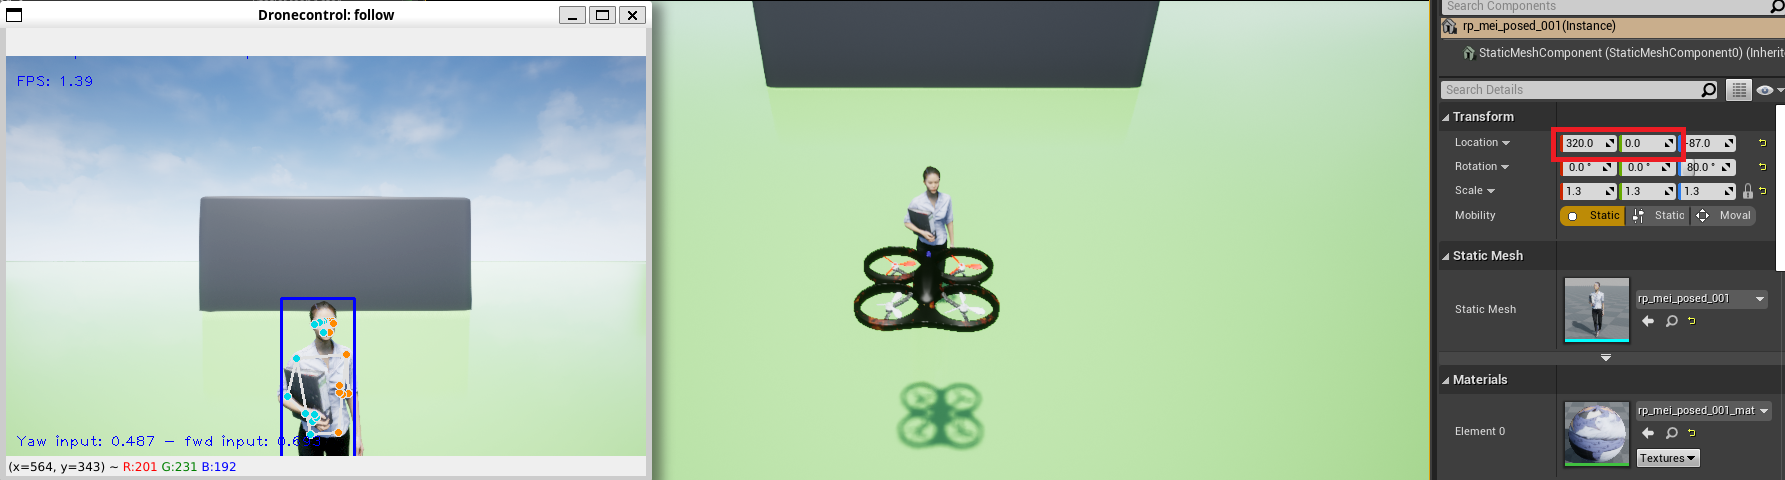
\includegraphics[width=\textwidth, keepaspectratio]{img/pid-3/tune-ref-pos-fwd.png}
  \caption{Starting position of the simulator for tuning the forward controller. The human model is situated \unit[420]{cm} forward and centred from the vehicle position.}\label{fig:tune-ref-pos-fwd}
\end{figure}

The process to select the component gains for the forward controller runs similarly to the yaw controller. The plotted outputs from the tuning utility are contained in Appendix \ref{app:fwd-pid-results}. Based on those graphs, the selected values for the parameters are $K_P=4$, $K_I=1$ and $K_D=0$.


\subsection{PID controller validation}
\label{subsec:pid-test-controller}

The chosen values for the controllers can now be applied to the complete follow solution to get a clearer picture of the expected performance of the vehicle during flight tests. In this test, the follow application is started, and the drone is made to take off and switch flight mode to offboard control. After the person is detected by the pose mechanisms, the 3D-model is moved around in the simulated world to observe how the vehicle reacts. The expected result is that the movement is appreciatively more responsive than on the follow test run with the non-tuned P-only controller at the end of Section \ref{sec:test-3-airsim} (\emph{Verify integration with follow solution}). To provide a visual demonstration, a video showcasing the test described can be accessed \href{https://l-gonz.github.io/tfg-giaa-dronecontrol/videos/test-sitl-follow}{here}\footnote{\url{https://l-gonz.github.io/tfg-giaa-dronecontrol/videos/test-sitl-follow}}. Additionally, Figure \ref{fig:airsim-test-follow} displays a frame extracted from the video, giving a glimpse of the drone's behaviour during the follow operation.

\begin{figure}[H]
  \centering
  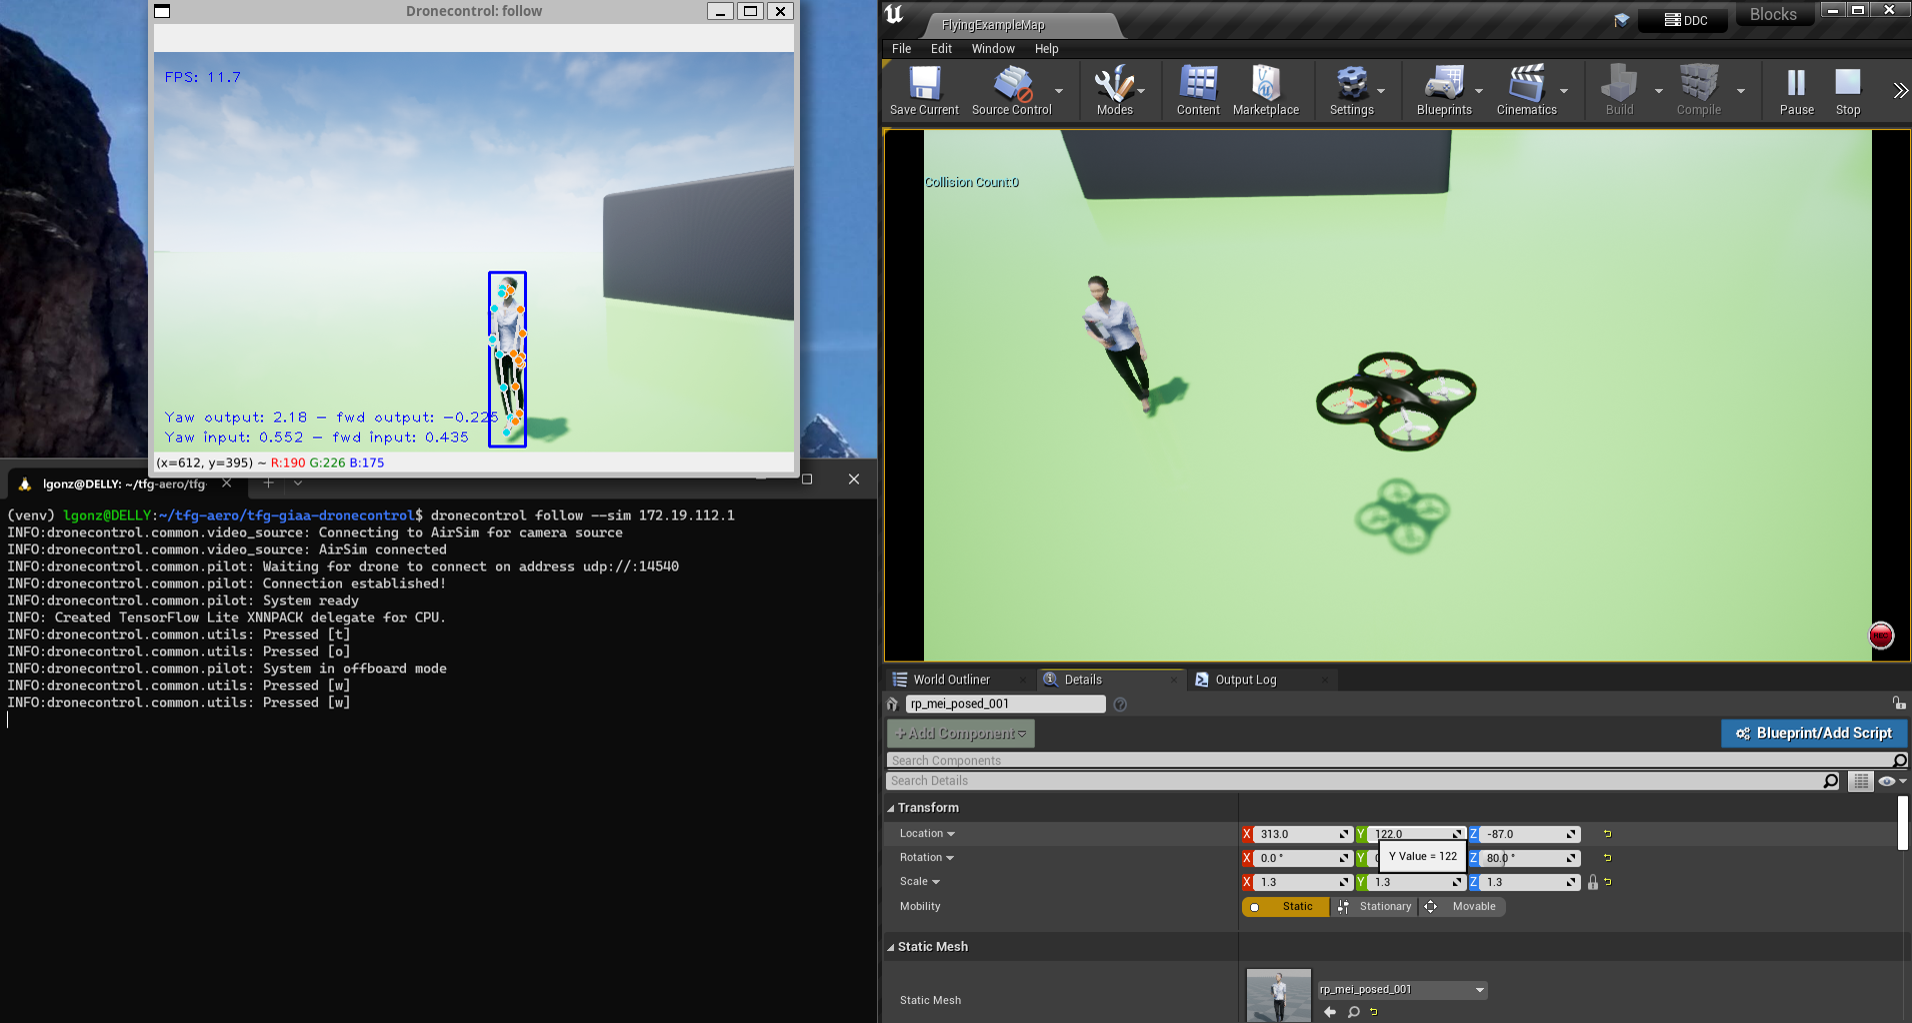
\includegraphics[width=\textwidth, keepaspectratio]{img/video-follow-sitl.png}
  \caption{Single frame from the video showing the movement of the drone in response to changes in the position of the tracked person.}\label{fig:airsim-test-follow}
\end{figure}

